\documentclass[8pt,a4paper,fancyhdr,hyperref,UTF8]{ctexbook}
\usepackage{multirow}
% for \soul 删除线
\usepackage{ulem}
\usepackage{amsmath}
% 表头斜线
\usepackage{diagbox}

\makeatletter
\usepackage[centering,paperwidth=210mm,paperheight=297mm,%
body={165mm,245mm},marginparsep=10pt,marginpar=50pt]{geometry}
\usepackage{color}
\usepackage{enumitem}
\usepackage{fancyvrb}
\usepackage[bottom,perpage,symbol*]{footmisc}
\usepackage{graphicx}
\usepackage[hidelinks]{hyperref}
\usepackage{makeidx}
\usepackage[toc]{multitoc}
\usepackage{pifont}
\usepackage{underscore}
\usepackage{amsmath}

\DefineFNsymbols*{chinese}{{\ding{172}}{\ding{173}}{\ding{174}}{\ding{175}}%
	{\ding{176}}{\ding{177}}{\ding{178}}{\ding{179}}{\ding{180}}{\ding{181}}}
\setfnsymbol{chinese}

\hypersetup{bookmarksnumbered=true,bookmarksdepth=2}

\CTEXsetup[number={\thechapter}]{chapter}
\CTEXsetup[format+={\raggedleft}]{chapter}
\CTEXsetup[beforeskip={10pt}]{chapter}
\CTEXsetup[afterskip={30pt}]{chapter}
\def\CTEX@chapter@aftername{\par} % \CTEXsetup[aftername={\par}]{chapter}
\CTEXsetup[format+={\raggedright}]{section}
\CTEXsetup[beforeskip={-3.0ex plus -1ex minus -.2ex}]{section}
\CTEXsetup[afterskip={2.3ex plus .2ex minus 0.2ex}]{section}

\renewcommand \thefigure{\thechapter-\arabic{figure}}
\renewcommand \thetable{\thechapter-\arabic{table}}

\newcommand\figcaption[1]{\def\@captype{figure}\caption{#1}}
\newcommand\tabcaption[1]{\def\@captype{table}\caption{#1}}

\long\def\@caption#1[#2]#3{%
	\addcontentsline{\csname ext@#1\endcsname}{#1}%
	{\protect\numberline{\csname fnum@#1\endcsname}{ \ignorespaces #2}}% change 
	%"the" to "fnum@"
	\normalsize
	\@makecaption{\csname fnum@#1\endcsname}{\ignorespaces #3}}

\long\def\@makecaption#1#2{%
	\vskip\abovecaptionskip
	\sbox\@tempboxa{#1\quad#2}%
	\ifdim \wd\@tempboxa >\hsize
	#1\quad#2\par
	\else
	\global \@minipagefalse
	\hb@xt@\hsize{\hfil\box\@tempboxa\hfil}%
	\fi
	\vskip\belowcaptionskip}

\setlength\abovecaptionskip{0pt}

%\setmainfont{Times New Roman}
\setmainfont{Linux Libertine}
%\setmainfont{TeX Gyre Pagella}
\newfontfamily\urlfont{PT Sans Narrow}
%\setmonofont[AutoFakeBold=1.6,AutoFakeSlant=0.17,Mapping=tex-text-tt]{Inconsolata}
\setCJKfamilyfont{zhyou}{YouYuan}

\newcommand{\fn}[1]{\texttt{#1}}
\newcommand{\sfn}[1]{\texttt{\small #1}}
\newcommand{\kw}[1]{\textsf{#1}}
\newcommand{\myurl}[1]{{\urlfont #1}}
\newcommand{\mpar}[1]{\marginpar[\hfill\kaishu #1]{\kaishu #1}}
\newcommand{\mn}[1]{\texttt{\bs #1}}
\renewcommand{\today}{\the\year-\the\month-\the\day}
\newcommand\bs{\textbackslash}
\newcommand{\code}[1]{\small{\fontspec{Latin Modern Mono} #1}}

\newcommand\begindot{\begin{itemize}
		[itemsep=2pt plus 2pt minus 2pt,%
		topsep=3pt plus 2pt minus 2pt,%
		parsep=0pt plus 2pt minus 2pt]}
	\newcommand\myenddot{\end{itemize}}

\newcommand\beginnum{\begin{enumerate}
		[itemsep=2pt plus 2pt minus 2pt,%
		topsep=3pt plus 2pt minus 2pt,%
		parsep=0pt plus 2pt minus 2pt]}
	\newcommand\myendnum{\end{enumerate}}

\DefineVerbatimEnvironment%
{Code}{Verbatim}
{tabsize=4,fontsize=\small,baselinestretch=1.0,xleftmargin=2mm}

\raggedbottom
%\setlength{\parskip}{1ex plus .5ex minus .5ex}

\def\FV@SetLineWidth{%
  \if@FV@ResetMargins\else
    \advance\leftmargin\@totalleftmargin
  \fi
  \advance\leftmargin\FV@XLeftMargin\relax
  \advance\rightmargin\FV@XRightMargin\relax
  \linewidth\hsize
  %\advance\linewidth-\leftmargin
  %\advance\linewidth-\rightmargin
  \hfuzz\FancyVerbHFuzz\relax}


\def\FV@SingleFrameLine#1{%
%% DG/SR modification end
  \hbox to\z@{%
    %\kern\leftmargin
%% DG/SR modification begin - Jun. 22, 1998
    \ifnum#1=\z@
      \let\FV@Label\FV@LabelBegin
    \else
      \let\FV@Label\FV@LabelEnd
    \fi
    \ifx\FV@Label\relax
%% DG/SR modification end
      \FancyVerbRuleColor{\vrule \@width\linewidth \@height\FV@FrameRule}%
%% DG/SR modification begin - Jun. 22, 1998
    \else
      \ifnum#1=\z@
        \setbox\z@\hbox{\strut\enspace\urlfont\FV@LabelBegin\strut}%
      \else
        \setbox\z@\hbox{\strut\enspace\urlfont\FV@LabelEnd\strut}%
      \fi
      \@tempdimb=\dp\z@
      \advance\@tempdimb -.5\ht\z@
      \@tempdimc=\linewidth
      \advance\@tempdimc -\wd\z@
      %\divide\@tempdimc\tw@
      \ifnum#1=\z@              % Top line
        \ifx\FV@LabelPositionTopLine\relax
          \FancyVerbRuleColor{\vrule \@width\linewidth \@height\FV@FrameRule}%
        \else
          \FV@FrameLineWithLabel
        \fi
      \else                     % Bottom line
        \ifx\FV@LabelPositionBottomLine\relax
          \FancyVerbRuleColor{\vrule \@width\linewidth \@height\FV@FrameRule}%
        \else
          \FV@FrameLineWithLabel
        \fi
      \fi
    \fi
%% DG/SR modification end
    \hss}}


%% DG/SR modification begin - May. 19, 1998
\def\FV@FrameLineWithLabel{%
  \ht\z@\@tempdimb\dp\z@\@tempdimb%
  \FancyVerbRuleColor{%
    \raise 0.5ex\hbox{\vrule \@width\@tempdimc \@height\FV@FrameRule}%
    \raise\@tempdimb\box\z@}}
%% DG/SR modification end


\def\FV@EndListFrame@Lines{%
  \begingroup
    %\vskip 0.5ex
    \baselineskip\z@skip
    \kern\FV@FrameSep\relax
%% DG/SR modification begin - May. 19, 1998
%%    \FV@SingleFrameLine
    \FV@SingleFrameLine{\@ne}%
%% DG/SR modification end
  \endgroup}

\newskip\mytopsep
\setlength{\mytopsep}{4pt plus 2pt minus 3pt}

\def\FV@ListVSpace{%
  \@topsepadd\mytopsep
  \if@noparlist\advance\@topsepadd\partopsep\fi
  \if@inlabel
    \vskip\parskip
  \else
    \if@nobreak
      \vskip\parskip
      \clubpenalty\@M
    \else
      \addpenalty\@beginparpenalty
      \@topsep\@topsepadd
      \advance\@topsep\parskip
      \addvspace\@topsep
    \fi
  \fi
  %\showthe \@topsepadd
  %\showthe \topsep
  %\showthe \partopsep
  %\showthe \parskip
  \global\@nobreakfalse
  \global\@inlabelfalse
  \global\@minipagefalse
  \global\@newlistfalse}

\def\FV@EndList{%
  \FV@ListProcessLastLine
  \FV@EndListFrame
  %\showthe \@topsepadd
  \@endparenv
  \endgroup
  \@endpetrue}

\def\theFancyVerbLine{\sffamily\scriptsize\arabic{FancyVerbLine}}

\DefineVerbatimEnvironment%
{Codex}{Verbatim}
{tabsize=4, 
fontsize=\small,baselinestretch=1.0,xleftmargin=2mm,frame=lines,labelposition=all,framesep=5pt}

\DefineVerbatimEnvironment%
{Code}{Verbatim}
{tabsize=4,fontsize=\small,baselinestretch=1.0,xleftmargin=2mm}

\makeindex
\makeatother

\begin{document}
\sloppy
\newcommand\BookTitle{Cracking the Coding Interview C++11}
\pagestyle{fancy}
\fancyhead[RE]{\normalfont\small\rmfamily\nouppercase{\leftmark}}
\fancyhead[LO]{\normalfont\small\rmfamily\nouppercase{\rightmark}}
\fancyhead[LE,RO]{\thepage}

\makeatletter
\@openrightfalse
\makeatother

\frontmatter % 开始前言目录,页码用罗马数字

\thispagestyle{plain}
\begin{center}
  {\LARGE\textbf{\BookTitle}}

  \vspace{1em}
  {\large 戴方勤 (soulmachine@gmail.com)}

  \vspace{1ex}
  \myurl{https://github.com/soulmachine/acm-cheat-sheet}
  
  \vspace{1ex}
  最后更新 \today
  
  \vspace{1em}
  \textbf{\large 版权声明}
\end{center}
\noindent 本作品采用“Creative Commons 署名-非商业性使用-相同方式共享 3.0 Unported许可协议 
(cc by-nc-sa)”进行许可。
\texttt{\small http://creativecommons.org/licenses/by-nc-sa/3.0/}

\vspace{1em}
\subsubsection{内容简介}
本书的目标读者是准备去北美找工作的码农,也适用于在国内找工作的码农,以及刚接触ACM算法竞赛的新手。

本书包含了一些经典题目的范例代码,经过精心编写,编码规范良好,适合在纸上默写。

怎么样才算是经典的算法题?一般经典的题目都有约定俗成的名称,例如“八皇后问题”,“0-1背包问题”等,这些名字已经固定下来了,类似于一个“成语”,一般说出名字,大家就都知道题目意思了,不用再解释题目内容,这就是所谓的“经典”。同时,本书的每一个题目,都至少在两本纸质书中出现过。

这本书的定位,与ACM算法竞赛类书籍不同。全书的题目比ACM竞赛简单,没有高难度的题目,但每道题目,都有详细生动的解释,还给出了可以直接在OJ上AC的代码。同时,题目的范围不限于算法竞赛,还包括了一些面试中常碰到的工程类题目。

全书的代码,使用“纯C + STL”的风格。本书中的代码规范,跟在公司中的工程规范略有不同,为了使代码短(方便迅速实现):

\begindot
\item 所有代码都是单一文件。这是因为一般OJ网站,提交代码的时候只有一个文本框,如果还是
按照标准做法,比如分为头文件.h和源代码.cpp,无法在网站上提交;

\item 喜欢在全局定义一个最大整数,例如MAX。一般的OJ题目,都会有数据规模的限制,所以定义
一个常量MAX表示这个规模,可以不用动态分配内存,让代码实现更简单;

\item 经常使用全局变量。比如用几个全局变量,定义某个递归函数需要的数据,减少递归函数的参数
个数,就减少了递归时栈内存的消耗,可以说这几个全局变量是这个递归函数的“环境”。

\item 不提倡防御式编程。不需要检查malloc()/new 返回的指针是否为NULL;不需要检查内部函数入口
参数的有效性;使用纯C基于对象编程时,调用对象的成员方法,不需要检查对象自身是否为NULL。
\myenddot

本手册假定读者已经学过《数据结构》\footnote{《数据结构》,严蔚敏等著,清华大学出版社,
\myurl{http://book.douban.com/subject/2024655/}},
《算法》\footnote{《Algorithms》,Robert Sedgewick, Addison-Wesley Professional, \myurl{http://book.douban.com/subject/4854123/}}
这两门课,熟练掌握C++或Java。

\subsubsection{Github地址}
本书是开源的,项目地址:\myurl{https://github.com/soulmachine/acm-cheat-sheet}

\subsubsection{北美求职微博群}
我和我的小伙伴们在这里:\myurl{http://q.weibo.com/1312378}


\tableofcontents

\mainmatter % 开始正文,页码用阿拉伯数字

\graphicspath{{diagrams/}}

\chapter{编程技巧}
较大的数组放在main函数外,作为全局变量,这样可以防止栈溢出,因为栈的大小是有限制的。
如果能够预估栈,队列的上限,则不要用\fn{stack, queue},使用数组来模拟,这样速度最快。
输入数据一般放在全局变量,且在运行过程中不要修改这些变量。


在判断两个浮点数 (i.e., 
float/double) 
a和b是否相等时,不应该用\fn{a==b},而是判断二者之差的绝对值\fn{fabs(a-b)}是否小于某个阀值 
\fn{$\epsilon$=1e-9}。

判断一个整数是否是为奇数,用\fn{x \% 2 != 0}或\fn{x \& 1 != 0},不要用\fn{x \% 2 == 
1},因为x可能是负数。

用\fn{char}的值作为数组下标(例如,统计字符串中每个字符出现的次数),要考虑到\fn{char}可能是负数。有的人考虑到了,先强制转型为\fn{unsigned
 int}再用作下标,这仍然是错的。正确的做法是,先强制转型为\fn{unsigned char},再用作下标。这涉及C++整型提升的规则,就不详述了。

以下是关于STL基于《Effective STL》的使用技巧。

\subsubsection{vector和string优先于动态分配的数组}
首先,在性能上,由于\fn{vector}能够保证连续内存,因此一旦分配了后,它的性能跟原始数组相当;

其次,如果用new,意味着你要确保后面进行了delete,一旦忘记了,就会出现BUG,且这样需要都写一行delete,代码不够短;

再次,声明多维数组的话,只能一个一个new,例如:
\begin{Code}
	int** ary = new int*[row_num];
	for(int i = 0; i < row_num; ++i)
		ary[i] = new int[col_num];
\end{Code}

用vector的话一行代码搞定,
\begin{Code}
	vector<vector<int> > ary(row_num, vector<int>(col_num, 0));
\end{Code}
\subsubsection{使用reserve来避免不必要的重新分配}
\subsubsection{用empty来代替检查size()是否为0}
\subsubsection{确保new|delete和malloc|free的成对出现, 
使用智能指针shared_ptr和unique_ptr,替代auto_ptr容器}
\subsubsection{用distance和advance把const_iterator转化成iterator}
\chapter{线性表}
线性表(Linear List)包含:
\begindot
\item 顺序存储:数组
\item 链式存储:单链表,双向链表,循环单链表,循环双向链表
\item 二者结合:静态链表
\myenddot

\section{数组} %%%%%%%%%%%%%%%%%%%%%%%%%%%%%%


\subsection{Remove Duplicates from Sorted Array}
\label{sec:remove-duplicates-from-sorted-array}


\subsubsection{描述}
Given a sorted array, remove the duplicates in place such that each element 
appear only once and return the new length.
Do not allocate extra space for another array, you must do this in place with 
constant memory.
For example, Given input array \code{A = [1,1,2]},
Your function should return length = 2, and A is now \code{[1,2]}.

\subsubsection{分析}
二指针问题,一前一后扫描。

\subsubsection{代码1}
\begin{Code}
	// LeetCode, Remove Duplicates from Sorted Array
	// 时间复杂度O(n),空间复杂度O(1)
	class Solution {
		int removeDuplicates(int A[], int n) {
			if (n==0 || A==nullptr) return 0;
			int index = 0;
			for (int i = 1; i < n; i++) {
				if (A[index] != A[i])
					A[++index] = A[i];
			}
			return index + 1;
		}
	};
\end{Code}
\subsubsection{代码2}
\begin{Code}
	// LeetCode, Remove Duplicates from Sorted Array
	// 使用STL,时间复杂度O(n),空间复杂度O(1)
	class Solution {
		int removeDuplicates(int A[], int n) {
			return distance(A, unique(A, A + n));
		}
	};
\end{Code}
\subsubsection{代码3}
\begin{Code}
	// LeetCode, Remove Duplicates from Sorted Array
	// 使用STL,时间复杂度O(n),空间复杂度O(1)
	class Solution {
		int removeDuplicates(int A[], int n) {
			return removeDuplicates(A, A + n, A) - A;
		}
		
		template<typename InIt, typename OutIt>
		OutIt removeDuplicates(InIt first, InIt last, OutIt output) {
			while (first != last) {
				*output++ = *first;
				first = upper_bound(first, last, *first);
			}
			return output;
		}
	};
\end{Code}

\subsubsection{相关题目}

\begindot
\item Remove Duplicates from Sorted Array II,见 \S 
\ref{sec:remove-duplicates-from-sorted-array-ii}
\myenddot


\subsection{Remove Duplicates from Sorted Array II}
\label{sec:remove-duplicates-from-sorted-array-ii}


\subsubsection{描述}
Follow up for "Remove Duplicates":
What if duplicates are allowed at most twice?
For example,
Given sorted array \code{A = [1,1,1,2,2,3]},
Your function should return length = 5, and A is now \code{[1,1,2,2,3]}

\subsubsection{分析}
加一个变量记录一下元素出现的次数即可。这题因为是已经排序的数组,所以一个变量即可解决。如果是没有排序的数组,则需要引入一个hashmap来记录出现次数。


\subsubsection{代码1}
\begin{Code}
	// LeetCode, Remove Duplicates from Sorted Array II
	// 时间复杂度O(n),空间复杂度O(1)
	// @author hex108 (https://github.com/hex108)
	class Solution {
		public:
		int removeDuplicates(int A[], int n) {
			if (n <= 2) return n;
			
			int index = 2;
			for (int i = 2; i < n; i++){
				if (A[i] != A[index - 2])
				A[index++] = A[i];
			}
			
			return index;
		}
	};
\end{Code}


\subsubsection{代码2}
下面是一个更简洁的版本。上面的代码略长,不过扩展性好一些,例如将\fn{occur < 2}改为\fn{occur 
< 3},就变成了允许重复最多3次。
\begin{Code}
	// LeetCode, Remove Duplicates from Sorted Array II
	// @author 虞航仲 (http://weibo.com/u/1666779725)
	// 时间复杂度O(n),空间复杂度O(1)
	class Solution {
		public:
		int removeDuplicates(int A[], int n) {
			int index = 0;
			for (int i = 0; i < n; ++i) {
				if (i > 0 && i < n - 1 && A[i] == A[i - 1] && A[i] == A[i + 1])
				continue;
				
				A[index++] = A[i];
			}
			return index;
		}
	};
\end{Code}


\subsubsection{相关题目}

\begindot
\item Remove Duplicates from Sorted Array,见 \S 
\ref{sec:remove-duplicates-from-sorted-array}
\myenddot


\subsection{Search in Rotated Sorted Array}
\label{sec:search-in-rotated-sorted-array}

\subsubsection{描述}
Suppose a sorted array is rotated at some pivot unknown to you beforehand.
(i.e., \code{0 1 2 4 5 6 7} might become \code{4 5 6 7 0 1 2}).
You are given a target value to search. If found in the array return its index, 
otherwise return -1.
You may assume no duplicate exists in the array.

\subsubsection{分析}
二分查找,难度主要在于左右边界的确定。


\subsubsection{代码}
\begin{Code}
	// LeetCode, Search in Rotated Sorted Array
	// 时间复杂度O(log n),空间复杂度O(1)
	class Solution {
		public:
		int search(int A[], int n, int target) {
			int first = 0, last = n;
			while (first != last) {
				const int mid = first  + (last - first) / 2;
				if (A[mid] == target)
				return mid;
				if (A[first] <= A[mid]) {
					if (A[first] <= target && target < A[mid])
					last = mid;
					else
					first = mid + 1;
				} else {
				if (A[mid] < target && target <= A[last-1])
				first = mid + 1;
				else
				last = mid;
			}
		}
		return -1;
	}
};
\end{Code}


\subsubsection{相关题目}

\begindot
\item Search in Rotated Sorted Array II,见 \S 
\ref{sec:search-in-rotated-sorted-array-ii}
\myenddot


\subsection{Search in Rotated Sorted Array II}
\label{sec:search-in-rotated-sorted-array-ii}


\subsubsection{描述}
Follow up for "Search in Rotated Sorted Array": What if \emph{duplicates} are 
allowed?

Would this affect the run-time complexity? How and why?

Write a function to determine if a given target is in the array.


\subsubsection{分析}
允许重复元素,则上一题中如果\fn{A[m]>=A[l]},那么\fn{[l,m]}为递增序列的假设就不能成立了,比如\code{[1,3,1,1,1]}。

如果\fn{A[m]>=A[l]}不能确定递增,那就把它拆分成两个条件:
\begindot
\item 若\fn{A[m]>A[l]},则区间\fn{[l,m]}一定递增
\item 若\fn{A[m]==A[l]} 确定不了,那就\fn{l++},往下看一步即可。
\myenddot

\subsubsection{代码}
\begin{Code}
	// LeetCode, Search in Rotated Sorted Array II
	// 时间复杂度O(n),空间复杂度O(1)
	class Solution {
		public:
		bool search(int A[], int n, int target) {
			int first = 0, last = n;
			while (first != last) {
				const int mid = first  + (last - first) / 2;
				if (A[mid] == target)
				return true;
				if (A[first] < A[mid]) {
					if (A[first] <= target && target < A[mid])
					last = mid;
					else
					first = mid + 1;
				} else if (A[first] > A[mid]) {
				if (A[mid] < target && target <= A[last-1])
				first = mid + 1;
				else
				last = mid;
			} else
			//skip duplicate one
			first++;
		}
		return false;
	}
};
\end{Code}


\subsubsection{相关题目}

\begindot
\item Search in Rotated Sorted Array,见 \S 
\ref{sec:search-in-rotated-sorted-array}
\myenddot


\subsection{Median of Two Sorted Arrays}
\label{sec:median-of-two-sorted-arrays}


\subsubsection{描述}
There are two sorted arrays A and B of size m and n respectively. Find the 
median of the two sorted arrays. The overall run time complexity should be 
$O(\log (m+n))$.


\subsubsection{分析}
这是一道非常经典的题。这题更通用的形式是,给定两个已经排序好的数组,找到两者所有元素中第$k$大的元素。

$O(m+n)$的解法比较直观,直接merge两个数组,然后求第$k$大的元素。

不过我们仅仅需要第$k$大的元素,是不需要“排序”这么复杂的操作的。可以用一个计数器,记录当前已经找到第$m$大的元素了。同时我们使用两个指针\fn{pA}和\fn{pB},分别指向A和B数组的第一个元素,使用类似于merge
 
sort的原理,如果数组A当前元素小,那么\fn{pA++},同时\fn{m++};如果数组B当前元素小,那么\fn{pB++},同时\fn{m++}。最终当$m$等于$k$的时候,就得到了我们的答案,$O(k)$时间,$O(1)$空间。但是,当$k$很接近$m+n$的时候,这个方法还是$O(m+n)$的。

有没有更好的方案呢?我们可以考虑从$k$入手。如果我们每次都能够删除一个一定在第$k$大元素之前的元素,那么我们需要进行$k$次。但是如果每次我们都删除一半呢?由于A和B都是有序的,我们应该充分利用这里面的信息,类似于二分查找,也是充分利用了“有序”。

假设A和B的元素个数都大于$k/2$,我们将A的第$k/2$个元素(即\fn{A[k/2-1]})和B的第$k/2$个元素(即\fn{B[k/2-1]})进行比较,有以下三种情况(为了简化这里先假设$k$为偶数,所得到的结论对于$k$是奇数也是成立的):
\begindot
\item \fn{A[k/2-1] == B[k/2-1]}
\item \fn{A[k/2-1] > B[k/2-1]}
\item \fn{A[k/2-1] < B[k/2-1]}
\myenddot

如果\fn{A[k/2-1] < B[k/2-1]},意味着\fn{A[0]}到\fn{A[k/2-1}的肯定在$A \cup B$的top 
k元素的范围内,换句话说,\fn{A[k/2-1}不可能大于$A \cup B$的第$k$大元素。留给读者证明。

因此,我们可以放心的删除A数组的这$k/2$个元素。同理,当\fn{A[k/2-1] > 
B[k/2-1]}时,可以删除B数组的$k/2$个元素。

当\fn{A[k/2-1] == 
B[k/2-1]}时,说明找到了第$k$大的元素,直接返回\fn{A[k/2-1]}或\fn{B[k/2-1]}即可。

因此,我们可以写一个递归函数。那么函数什么时候应该终止呢?
\begindot
\item 当A或B是空时,直接返回\fn{B[k-1]}或\fn{A[k-1]};
\item 当\fn{k=1}是,返回\fn{min(A[0], B[0])};
\item 当\fn{A[k/2-1] == B[k/2-1]}时,返回\fn{A[k/2-1]}或\fn{B[k/2-1]}
\myenddot


\subsubsection{代码}
\begin{Code}
	// LeetCode, Median of Two Sorted Arrays
	// 时间复杂度O(log(m+n)),空间复杂度O(log(m+n))
	class Solution {
		public:
		double findMedianSortedArrays(int A[], int m, int B[], int n) {
			int total = m + n;
			if (total & 0x1)
			return find_kth(A, m, B, n, total / 2 + 1);
			else
			return (find_kth(A, m, B, n, total / 2)
			+ find_kth(A, m, B, n, total / 2 + 1)) / 2.0;
		}
		private:
		static int find_kth(int A[], int m, int B[], int n, int k) {
			//always assume that m is equal or smaller than n
			if (m > n) return find_kth(B, n, A, m, k);
			if (m == 0) return B[k - 1];
			if (k == 1) return min(A[0], B[0]);
			
			//divide k into two parts
			int ia = min(k / 2, m), ib = k - ia;
			if (A[ia - 1] < B[ib - 1])
			return find_kth(A + ia, m - ia, B, n, k - ia);
			else if (A[ia - 1] > B[ib - 1])
			return find_kth(A, m, B + ib, n - ib, k - ib);
			else
			return A[ia - 1];
		}
	};
\end{Code}


\subsubsection{相关题目}

\begindot
\item 无
\myenddot


\subsection{Longest Consecutive Sequence} %%%%%%%%%%%%%%%%%%%%%%%%%%%%%%
\label{sec:longest-consecutive-sequence}


\subsubsection{描述}
Given an unsorted array of integers, find the length of the longest consecutive 
elements sequence.

For example,
Given \code{[100, 4, 200, 1, 3, 2]},
The longest consecutive elements sequence is \code{[1, 2, 3, 4]}. Return its 
length: 4.

Your algorithm should run in $O(n)$ complexity.


\subsubsection{分析}
如果允许$O(n \log n)$的复杂度,那么可以先排序,可是本题要求$O(n)$。

由于序列里的元素是无序的,又要求$O(n)$,首先要想到用哈希表。

用一个哈希表 \fn{unordered_map<int, bool> 
used}记录每个元素是否使用,对每个元素,以该元素为中心,往左右扩张,直到不连续为止,记录下最长的长度。


\subsubsection{代码}
\begin{Code}
	// Leet Code, Longest Consecutive Sequence
	// 时间复杂度O(n),空间复杂度O(n)
	class Solution {
		public:
		int longestConsecutive(const vector<int> &num) {
			unordered_map<int, bool> used;
			
			for (auto i : num) used[i] = false;
			
			int longest = 0;
			
			for (auto i : num) {
				if (used[i]) continue;
				
				int length = 1;
				
				used[i] = true;
				
				for (int j = i + 1; used.find(j) != used.end(); ++j) {
					used[j] = true;
					++length;
				}
				
				for (int j = i - 1; used.find(j) != used.end(); --j) {
					used[j] = true;
					++length;
				}
				
				longest = max(longest, length);
			}
			
			return longest;
		}
	};
\end{Code}

\subsubsection{分析2}
第一直觉是个聚类的操作,应该有union,find的操作.连续序列可以用两端和长度来表示.
本来用两端就可以表示,但考虑到查询的需求,将两端分别暴露出来.用\fn{unordered_map<int, int> 
map}来
存储.原始思路来自于\url{http://discuss.leetcode.com/questions/1070/longest-consecutive-sequence}

\subsubsection{代码}

\begin{Code}
	// Leet Code, Longest Consecutive Sequence
	// 时间复杂度O(n),空间复杂度O(n)
	// Author: @advancedxy
	class Solution {
		public:
		int longestConsecutive(vector<int> &num) {
			unordered_map<int, int> map;
			int size = num.size();
			int l = 1;
			for (int i = 0; i < size; i++) {
				if (map.find(num[i]) != map.end()) continue;
				map[num[i]] = 1;
				if (map.find(num[i] - 1) != map.end()) {
					l = max(l, mergeCluster(map, num[i] - 1, num[i]));
				}
				if (map.find(num[i] + 1) != map.end()) {
					l = max(l, mergeCluster(map, num[i], num[i] + 1));
				}
			}
			return size == 0 ? 0 : l;
		}
		
		private:
		int mergeCluster(unordered_map<int, int> &map, int left, int right) {
			int upper = right + map[right] - 1;
			int lower = left - map[left] + 1;
			int length = upper - lower + 1;
			map[upper] = length;
			map[lower] = length;
			return length;
		}
	};
\end{Code}

\subsubsection{相关题目}
\begindot
\item 无
\myenddot


\subsection{Two Sum} %%%%%%%%%%%%%%%%%%%%%%%%%%%%%%
\label{sec:Two-sum}


\subsubsection{描述}
Given an array of integers, find two numbers such that they add up to a 
specific target number.

The function twoSum should return indices of the two numbers such that they add 
up to the target, where index1 must be less than index2. Please note that your 
returned answers (both index1 and index2) are not zero-based.

You may assume that each input would have exactly one solution.

Input:  \code{numbers=\{2, 7, 11, 15\}, target=9}

Output: \code{index1=1, index2=2}


\subsubsection{分析}
方法1:暴力,复杂度$O(n^2)$,会超时

方法2:hash。用一个哈希表,存储每个数对应的下标,复杂度$O(n)$.

方法3:先排序,然后左右夹逼,排序$O(n\log n)$,左右夹逼$O(n)$,最终$O(n\log 
n)$。但是注意,这题需要返回的是下标,而不是数字本身,因此这个方法行不通。


\subsubsection{代码}
\begin{Code}
	//LeetCode, Two Sum
	// 方法2:hash。用一个哈希表,存储每个数对应的下标
	// 时间复杂度O(n),空间复杂度O(n)
	class Solution {
		public:
		vector<int> twoSum(vector<int> &num, int target) {
			unordered_map<int, int> mapping;
			vector<int> result;
			for (int i = 0; i < num.size(); i++) {
				mapping[num[i]] = i;
			}
			for (int i = 0; i < num.size(); i++) {
				const int gap = target - num[i];
				if (mapping.find(gap) != mapping.end() && mapping[gap] > i) {
					result.push_back(i + 1);
					result.push_back(mapping[gap] + 1);
					break;
				}
			}
			return result;
		}
	};
\end{Code}


\subsubsection{相关题目}
\begindot
\item 3Sum, 见 \S \ref{sec:3sum}
\item 3Sum Closest, 见 \S \ref{sec:3sum-closest}
\item 4Sum, 见 \S \ref{sec:4sum}
\myenddot


\subsection{3Sum} %%%%%%%%%%%%%%%%%%%%%%%%%%%%%%
\label{sec:3sum}


\subsubsection{描述}
Given an array $S$ of $n$ integers, are there elements $a, b, c$ in $S$ such 
that $a + b + c = 0$? Find all unique triplets in the array which gives the sum 
of zero.

Note:
\begindot
\item Elements in a triplet $(a,b,c)$ must be in non-descending order. (ie, $a 
\leq b \leq c$)
\item The solution set must not contain duplicate triplets.
\myenddot

For example, given array \code{S = \{-1 0 1 2 -1 -4\}}.

A solution set is:
\begin{Code}
	(-1, 0, 1)
	(-1, -1, 2)
\end{Code}


\subsubsection{分析}
先排序,然后左右夹逼,复杂度 $O(n^2)$。

这个方法可以推广到$k$-sum,先排序,然后做$k-2$次循环,在最内层循环左右夹逼,时间复杂度是 
$O(\max\{n \log n, n^{k-1}\})$。


\subsubsection{代码}
\begin{Code}
	// LeetCode, 3Sum
	// 先排序,然后左右夹逼,时间复杂度O(n^2),空间复杂度O(1)
	class Solution {
		public:
		vector<vector<int>> threeSum(vector<int>& num) {
			vector<vector<int>> result;
			if (num.size() < 3) return result;
			sort(num.begin(), num.end());
			const int target = 0;
			
			auto last = num.end();
			for (auto a = num.begin(); a < prev(last, 2); ++a) {
				auto b = next(a);
				auto c = prev(last);
				while (b < c) {
					if (*a + *b + *c < target) {
						++b;
					} else if (*a + *b + *c > target) {
					--c;
				} else {
				result.push_back({ *a, *b, *c });
				++b;
				--c;
			}
		}
	}
	sort(result.begin(), result.end());
	result.erase(unique(result.begin(), result.end()), result.end());
	return result;
}
};
\end{Code}


\subsubsection{相关题目}
\begindot
\item Two sum, 见 \S \ref{sec:Two-sum}
\item 3Sum Closest, 见 \S \ref{sec:3sum-closest}
\item 4Sum, 见 \S \ref{sec:4sum}
\myenddot

\subsection{3Sum Closest} %%%%%%%%%%%%%%%%%%%%%%%%%%%%%%
\label{sec:3sum-closest}


\subsubsection{描述}
Given an array $S$ of $n$ integers, find three integers in $S$ such that the 
sum is closest to a given number, target. Return the sum of the three integers. 
You may assume that each input would have exactly one solution.

For example, given array \code{S = \{-1 2 1 -4\}}, and \code{target = 1}.

The sum that is closest to the target is 2. (\code{-1 + 2 + 1 = 2}).


\subsubsection{分析}
先排序,然后左右夹逼,复杂度 $O(n^2)$。


\subsubsection{代码}
\begin{Code}
	// LeetCode, 3Sum Closest
	// 先排序,然后左右夹逼,时间复杂度O(n^2),空间复杂度O(1)
	class Solution {
		public:
		int threeSumClosest(vector<int>& num, int target) {
			int result = 0;
			int min_gap = INT_MAX;
			
			sort(num.begin(), num.end());
			
			for (auto a = num.begin(); a != prev(num.end(), 2); ++a) {
				auto b = next(a);
				auto c = prev(num.end());
				
				while (b < c) {
					const int sum = *a + *b + *c;
					const int gap = abs(sum - target);
					
					if (gap < min_gap) {
						result = sum;
						min_gap = gap;
					}
					
					if (sum < target) ++b;
					else              --c;
				}
			}
			
			return result;
		}
	};
\end{Code}


\subsubsection{相关题目}
\begindot
\item Two sum, 见 \S \ref{sec:Two-sum}
\item 3Sum, 见 \S \ref{sec:3sum}
\item 4Sum, 见 \S \ref{sec:4sum}
\myenddot


\subsection{4Sum} %%%%%%%%%%%%%%%%%%%%%%%%%%%%%%
\label{sec:4sum}


\subsubsection{描述}
Given an array $S$ of $n$ integers, are there elements $a, b, c$, and $d$ in 
$S$ such that $a + b + c + d = target$? Find all unique quadruplets in the 
array which gives the sum of target.

Note:
\begindot
\item Elements in a quadruplet $(a,b,c,d)$ must be in non-descending order. 
(ie, $a \leq b \leq c \leq d$)
\item The solution set must not contain duplicate quadruplets.
\myenddot

For example, given array \code{S = \{1 0 -1 0 -2 2\}}, and \code{target = 0}. 

A solution set is:
\begin{Code}
	(-1,  0, 0, 1)
	(-2, -1, 1, 2)
	(-2,  0, 0, 2)
\end{Code}


\subsubsection{分析}
先排序,然后左右夹逼,复杂度 $O(n^3)$,会超时。

可以用一个hashmap先缓存两个数的和,最终复杂度$O(n^3)$。这个策略也适用于 3Sum 。


\subsubsection{左右夹逼}
\begin{Code}
	// LeetCode, 4Sum
	// 先排序,然后左右夹逼,时间复杂度O(n^3),空间复杂度O(1)
	class Solution {
		public:
		vector<vector<int>> fourSum(vector<int>& num, int target) {
			vector<vector<int>> result;
			if (num.size() < 4) return result;
			sort(num.begin(), num.end());
			
			auto last = num.end();
			for (auto a = num.begin(); a < prev(last, 3); ++a) {
				for (auto b = next(a); b < prev(last, 2); ++b) {
					auto c = next(b);
					auto d = prev(last);
					while (c < d) {
						if (*a + *b + *c + *d < target) {
							++c;
						} else if (*a + *b + *c + *d > target) {
						--d;
					} else {
					result.push_back({ *a, *b, *c, *d });
					++c;
					--d;
				}
			}
		}
	}
	sort(result.begin(), result.end());
	result.erase(unique(result.begin(), result.end()), result.end());
	return result;
}
};
\end{Code}


\subsubsection{map做缓存}
\begin{Code}
	// LeetCode, 4Sum
	// 用一个hashmap先缓存两个数的和
	// 时间复杂度,平均O(n^2),最坏O(n^4),空间复杂度O(n^2)
	class Solution {
		public:
		vector<vector<int> > fourSum(vector<int> &num, int target) {
			vector<vector<int>> result;
			if (num.size() < 4) return result;
			sort(num.begin(), num.end());
			
			unordered_map<int, vector<pair<int, int> > > cache;
			for (size_t a = 0; a < num.size(); ++a) {
				for (size_t b = a + 1; b < num.size(); ++b) {
					cache[num[a] + num[b]].push_back(pair<int, int>(a, b));
				}
			}
			
			for (int c = 0; c < num.size(); ++c) {
				for (size_t d = c + 1; d < num.size(); ++d) {
					const int key = target - num[c] - num[d];
					if (cache.find(key) == cache.end()) continue;
					
					const auto& vec = cache[key];
					for (size_t k = 0; k < vec.size(); ++k) {
						if (c <= vec[k].second)
						continue; // 有重叠
						
						result.push_back( { num[vec[k].first],
							num[vec[k].second], num[c], num[d] });
					}
				}
			}
			sort(result.begin(), result.end());
			result.erase(unique(result.begin(), result.end()), result.end());
			return result;
		}
	};
\end{Code}


\subsubsection{multimap}
\begin{Code}
	// LeetCode, 4Sum
	// 用一个 hashmap 先缓存两个数的和
	// 时间复杂度O(n^2),空间复杂度O(n^2)
	// @author 龚陆安(http://weibo.com/luangong)
	class Solution {
		public:
		vector<vector<int>> fourSum(vector<int>& num, int target) {
			vector<vector<int>> result;
			if (num.size() < 4) return result;
			sort(num.begin(), num.end());
			
			unordered_multimap<int, pair<int, int>> cache;
			for (int i = 0; i + 1 < num.size(); ++i)
			for (int j = i + 1; j < num.size(); ++j)
			cache.insert(make_pair(num[i] + num[j], make_pair(i, j)));
			
			for (auto i = cache.begin(); i != cache.end(); ++i) {
				int x = target - i->first;
				auto range = cache.equal_range(x);
				for (auto j = range.first; j != range.second; ++j) {
					auto a = i->second.first;
					auto b = i->second.second;
					auto c = j->second.first;
					auto d = j->second.second;
					if (a != c && a != d && b != c && b != d) {
						vector<int> vec = { num[a], num[b], num[c], num[d] };
						sort(vec.begin(), vec.end());
						result.push_back(vec);
					}
				}
			}
			sort(result.begin(), result.end());
			result.erase(unique(result.begin(), result.end()), result.end());
			return result;
		}
	};
\end{Code}


\subsubsection{方法4}
\begin{Code}
	// LeetCode, 4Sum
	// 先排序,然后左右夹逼,时间复杂度O(n^3logn),空间复杂度O(1),会超时
	// 跟方法1相比,表面上优化了,实际上更慢了,切记!
	class Solution {
		public:
		vector<vector<int>> fourSum(vector<int>& num, int target) {
			vector<vector<int>> result;
			if (num.size() < 4) return result;
			sort(num.begin(), num.end());
			
			auto last = num.end();
			for (auto a = num.begin(); a < prev(last, 3);
			a = upper_bound(a, prev(last, 3), *a)) {
				for (auto b = next(a); b < prev(last, 2);
				b = upper_bound(b, prev(last, 2), *b)) {
					auto c = next(b);
					auto d = prev(last);
					while (c < d) {
						if (*a + *b + *c + *d < target) {
							c = upper_bound(c, d, *c);
						} else if (*a + *b + *c + *d > target) {
						d = prev(lower_bound(c, d, *d));
					} else {
					result.push_back({ *a, *b, *c, *d });
					c = upper_bound(c, d, *c);
					d = prev(lower_bound(c, d, *d));
				}
			}
		}
	}
	return result;
}
};
\end{Code}


\subsubsection{相关题目}
\begindot
\item Two sum, 见 \S \ref{sec:Two-sum}
\item 3Sum, 见 \S \ref{sec:3sum}
\item 3Sum Closest, 见 \S \ref{sec:3sum-closest}
\myenddot


\subsection{Remove Element} %%%%%%%%%%%%%%%%%%%%%%%%%%%%%%
\label{sec:remove-element }


\subsubsection{描述}
Given an array and a value, remove all instances of that value in place and 
return the new length.

The order of elements can be changed. It doesn't matter what you leave beyond 
the new length.


\subsubsection{分析}
无


\subsubsection{代码1}
\begin{Code}
	// LeetCode, Remove Element
	// 时间复杂度O(n),空间复杂度O(1)
	class Solution {
		public:
		int removeElement(int A[], int n, int elem) {
			int index = 0;
			for (int i = 0; i < n; ++i) {
				if (A[i] != elem) {
					A[index++] = A[i];
				}
			}
			return index;
		}
	};
\end{Code}


\subsubsection{代码2}
\begin{Code}
	// LeetCode, Remove Element
	// 使用remove(),时间复杂度O(n),空间复杂度O(1)
	class Solution {
		public:
		int removeElement(int A[], int n, int elem) {
			return distance(A, remove(A, A+n, elem));
		}
	};
\end{Code}


\subsubsection{相关题目}
\begindot
\item 无
\myenddot


\subsection{Next Permutation} %%%%%%%%%%%%%%%%%%%%%%%%%%%%%%
\label{sec:next-permutation}


\subsubsection{描述}
Implement next permutation, which rearranges numbers into the lexicographically 
next greater permutation of numbers.

If such arrangement is not possible, it must rearrange it as the lowest 
possible order (ie, sorted in ascending order).

The replacement must be in-place, do not allocate extra memory.

Here are some examples. Inputs are in the left-hand column and its 
corresponding outputs are in the right-hand column.
\begin{Code}
	1,2,3 → 1,3,2
	3,2,1 → 1,2,3
	1,1,5 → 1,5,1
\end{Code}


\subsubsection{分析}
算法过程如图~\ref{fig:permutation}所示(来自\myurl{http://fisherlei.blogspot.com/2012/12/leetcode-next-permutation.html})。

\begin{center}
	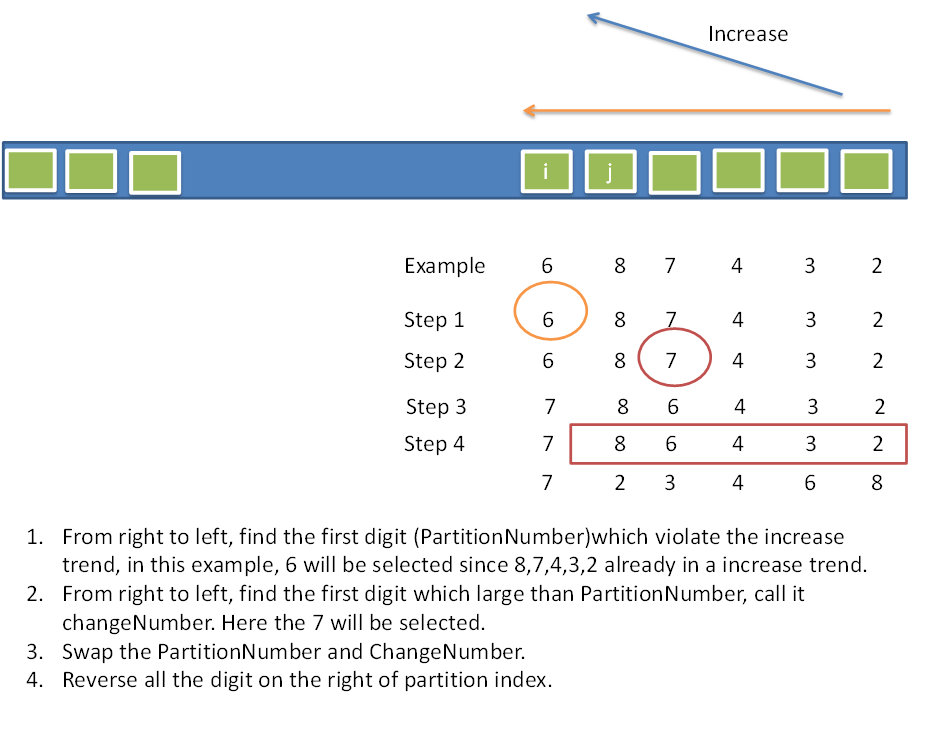
\includegraphics[width=360pt]{next-permutation.png}\\
	\figcaption{下一个排列算法流程}\label{fig:permutation}
\end{center}


\subsubsection{代码}
\begin{Code}
	// LeetCode, Next Permutation
	// 时间复杂度O(n),空间复杂度O(1)
	class Solution {
		public:
		void nextPermutation(vector<int> &num) {
			next_permutation(num.begin(), num.end());
		}
		
		template<typename BidiIt>
		bool next_permutation(BidiIt first, BidiIt last) {
			// Get a reversed range to simplify reversed traversal.
			const auto rfirst = reverse_iterator<BidiIt>(last);
			const auto rlast = reverse_iterator<BidiIt>(first);
			
			// Begin from the second last element to the first element.
			auto pivot = next(rfirst);
			
			// Find `pivot`, which is the first element that is no less than its
			// successor.  `Prev` is used since `pivort` is a 
			`reversed_iterator`.
			while (pivot != rlast && *pivot >= *prev(pivot))
			++pivot;
			
			// No such elemenet found, current sequence is already the largest
			// permutation, then rearrange to the first permutation and return 
			false.
			if (pivot == rlast) {
				reverse(rfirst, rlast);
				return false;
			}
			
			// Scan from right to left, find the first element that is greater 
			than
			// `pivot`.
			auto change = find_if(rfirst, pivot, bind1st(less<int>(), *pivot));
			
			swap(*change, *pivot);
			reverse(rfirst, pivot);
			
			return true;
		}
	};
\end{Code}


\subsubsection{相关题目}
\begindot
\item Permutation Sequence, 见 \S \ref{sec:permutation-sequence}
\item Permutations, 见 \S \ref{sec:permutations}
\item Permutations II, 见 \S \ref{sec:permutations-ii}
\item Combinations, 见 \S \ref{sec:combinations}
\myenddot


\subsection{Permutation Sequence} %%%%%%%%%%%%%%%%%%%%%%%%%%%%%%
\label{sec:permutation-sequence}


\subsubsection{描述}
The set \fn{[1,2,3,…,n]} contains a total of $n!$ unique permutations.

By listing and labeling all of the permutations in order,
We get the following sequence (ie, for $n = 3$):
\begin{Code}
	"123"
	"132"
	"213"
	"231"
	"312"
	"321"
\end{Code}

Given $n$ and $k$, return the kth permutation sequence.

Note: Given $n$ will be between 1 and 9 inclusive.


\subsubsection{分析}
简单的,可以用暴力枚举法,调用 $k-1$ 次 \fn{next_permutation()}。

暴力枚举法把前 $k$个排列都求出来了,比较浪费,而我们只需要第$k$个排列。

利用康托编码的思路,假设有$n$个不重复的元素,第$k$个排列是$a_1, a_2, a_3, ..., 
a_n$,那么$a_1$是哪一个位置呢?

我们把$a_1$去掉,那么剩下的排列为
$a_2, a_3, ..., a_n$, 共计$n-1$个元素,$n-1$个元素共有$(n-1)!$个排列,于是就可以知道 
$a_1 = k / (n-1)!$。

同理,$a_2, a_3, ..., a_n$的值推导如下:

\begin{eqnarray}
	k_2 &=& k\%(n-1)! \nonumber \\
	a_2 &=& k_2/(n-2)! \nonumber \\
	\quad & \cdots \nonumber \\
	k_{n-1} &=& k_{n-2}\%2! \nonumber \\
	a_{n-1} &=& k_{n-1}/1! \nonumber \\
	a_n &=& 0 \nonumber
\end{eqnarray}


\subsubsection{使用next_permutation()}
\begin{Code}
	// LeetCode, Permutation Sequence
	// 使用next_permutation(),TLE
	class Solution {
		public:
		string getPermutation(int n, int k) {
			string s(n, '0');
			for (int i = 0; i < n; ++i)
			s[i] += i+1;
			for (int i = 0; i < k-1; ++i)
			next_permutation(s.begin(), s.end());
			return s;
		}
		
		template<typename BidiIt>
		bool next_permutation(BidiIt first, BidiIt last) {
			// 代码见上一题 Next Permutation
		}
	};
\end{Code}


\subsubsection{康托编码}
\begin{Code}
	// LeetCode, Permutation Sequence
	// 康托编码,时间复杂度O(n),空间复杂度O(1)
	class Solution {
		public:
		string getPermutation(int n, int k) {
			string s(n, '0');
			string result;
			for (int i = 0; i < n; ++i)
			s[i] += i + 1;
			
			return kth_permutation(s, k);
		}
		private:
		int factorial(int n) {
			int result = 1;
			for (int i = 1; i <= n; ++i)
			result *= i;
			return result;
		}
		
		// seq 已排好序,是第一个排列
		template<typename Sequence>
		Sequence kth_permutation(const Sequence &seq, int k) {
			const int n = seq.size();
			Sequence S(seq);
			Sequence result;
			
			int base = factorial(n - 1);
			--k;  // 康托编码从0开始
			
			for (int i = n - 1; i > 0; k %= base, base /= i, --i) {
			auto a = next(S.begin(), k / base);
			result.push_back(*a);
			S.erase(a);
		}
		
		result.push_back(S[0]); // 最后一个
		return result;
	}
};
\end{Code}


\subsubsection{相关题目}
\begindot
\item Next Permutation, 见 \S \ref{sec:next-permutation}
\item Permutations, 见 \S \ref{sec:permutations}
\item Permutations II, 见 \S \ref{sec:permutations-ii}
\item Combinations, 见 \S \ref{sec:combinations}
\myenddot


\subsection{Valid Sudoku} %%%%%%%%%%%%%%%%%%%%%%%%%%%%%%
\label{sec:valid-sudoku}


\subsubsection{描述}
Determine if a Sudoku is valid, according to: Sudoku Puzzles - The Rules 
\myurl{http://sudoku.com.au/TheRules.aspx} .

The Sudoku board could be partially filled, where empty cells are filled with 
the character \fn{'.'}.

\begin{center}
	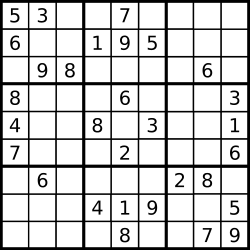
\includegraphics[width=150pt]{sudoku.png}\\
	\figcaption{A partially filled sudoku which is valid}\label{fig:sudoku}
\end{center}

\subsubsection{分析}
细节实现题。


\subsubsection{代码}
\begin{Code}
	// LeetCode, Valid Sudoku
	// 时间复杂度O(n^2),空间复杂度O(1)
	class Solution {
		public:
		bool isValidSudoku(const vector<vector<char>>& board) {
			bool used[9];
			
			for (int i = 0; i < 9; ++i) {
				fill(used, used + 9, false);
				
				for (int j = 0; j < 9; ++j) // 检查行
				if (!check(board[i][j], used))
				return false;
				
				fill(used, used + 9, false);
				
				for (int j = 0; j < 9; ++j) // 检查列
				if (!check(board[j][i], used))
				return false;
			}
			
			for (int r = 0; r < 3; ++r) // 检查 9 个子格子
			for (int c = 0; c < 3; ++c) {
				fill(used, used + 9, false);
				
				for (int i = r * 3; i < r * 3 + 3; ++i)
				for (int j = c * 3; j < c * 3 + 3; ++j)
				if (!check(board[i][j], used))
				return false;
			}
			
			return true;
		}
		
		bool check(char ch, bool used[9]) {
			if (ch == '.') return true;
			
			if (used[ch - '1']) return false;
			
			return used[ch - '1'] = true;
		}
	};
\end{Code}


\subsubsection{相关题目}
\begindot
\item Sudoku Solver, 见 \S \ref{sec:sudoku-solver}
\myenddot


\subsection{Trapping Rain Water} %%%%%%%%%%%%%%%%%%%%%%%%%%%%%%
\label{sec:trapping-rain-water}


\subsubsection{描述}
Given $n$ non-negative integers representing an elevation map where the width 
of each bar is 1, compute how much water it is able to trap after raining.

For example, 
Given \code{[0,1,0,2,1,0,1,3,2,1,2,1]}, return 6.

\begin{center}
	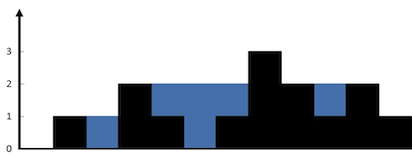
\includegraphics{trapping-rain-water.png}\\
	\figcaption{Trapping Rain Water}\label{fig:trapping-rain-water}
\end{center}


\subsubsection{分析}
对于每个柱子,找到其左右两边最高的柱子,该柱子能容纳的面积就是\code{min(max_left, 
max_right) - height}。所以,
\begin{enumerate}
	\item 从左往右扫描一遍,对于每个柱子,求取左边最大值;
	\item 从右往左扫描一遍,对于每个柱子,求最大右值;
	\item 再扫描一遍,把每个柱子的面积并累加。
\end{enumerate}

也可以,
\begin{enumerate}
	\item 扫描一遍,找到最高的柱子,这个柱子将数组分为两半;
	\item 处理左边一半;
	\item 处理右边一半。
\end{enumerate}


\subsubsection{代码1}
\begin{Code}
	// LeetCode, Trapping Rain Water
	// 思路1,时间复杂度O(n),空间复杂度O(n)
	class Solution {
		public:
		int trap(int A[], int n) {
			int *max_left = new int[n]();
			int *max_right = new int[n]();
			
			for (int i = 1; i < n; i++) {
				max_left[i] = max(max_left[i - 1], A[i - 1]);
				max_right[n - 1 - i] = max(max_right[n - i], A[n - i]);
				
			}
			
			int sum = 0;
			for (int i = 0; i < n; i++) {
				int height = min(max_left[i], max_right[i]);
				if (height > A[i]) {
					sum += height - A[i];
				}
			}
			
			delete[] max_left;
			delete[] max_right;
			return sum;
		}
	};
\end{Code}


\subsubsection{代码2}
\begin{Code}
	// LeetCode, Trapping Rain Water
	// 思路2,时间复杂度O(n),空间复杂度O(1)
	class Solution {
		public:
		int trap(int A[], int n) {
			int max = 0; // 最高的柱子,将数组分为两半
			for (int i = 0; i < n; i++)
			if (A[i] > A[max]) max = i;
			
			int water = 0;
			for (int i = 0, peak = 0; i < max; i++)
			if (A[i] > peak) peak = A[i];
			else water += peak - A[i];
			for (int i = n - 1, top = 0; i > max; i--)
			if (A[i] > top) top = A[i];
			else water += top - A[i];
			return water;
		}
	};
\end{Code}


\subsubsection{代码3}
第三种解法,用一个栈辅助,小于栈顶的元素压入,大于等于栈顶就把栈里所有小于或等于当前值的元素全部出栈处理掉。
\begin{Code}
	// LeetCode, Trapping Rain Water
	// 用一个栈辅助,小于栈顶的元素压入,大于等于栈顶就把栈里所有小于或
	// 等于当前值的元素全部出栈处理掉,计算面积,最后把当前元素入栈
	// 时间复杂度O(n),空间复杂度O(n)
	class Solution {
		public:
		int trap(int a[], int n) {
			stack<pair<int, int>> s;
			int water = 0;
			
			for (int i = 0; i < n; ++i) {
				int height = 0;
				
				while (!s.empty()) { // 将栈里比当前元素矮或等高的元素全部处理掉
					int bar = s.top().first;
					int pos = s.top().second;
					// bar, height, a[i] 三者夹成的凹陷
					water += (min(bar, a[i]) - height) * (i - pos - 1);
					height = bar;
					
					if (a[i] < bar) // 碰到了比当前元素高的,跳出循环
					break;
					else
					s.pop(); // 弹出栈顶,因为该元素处理完了,不再需要了
				}
				
				s.push(make_pair(a[i], i));
			}
			
			return water;
		}
	};
\end{Code}


\subsubsection{相关题目}
\begindot
\item Container With Most Water, 见 \S \ref{sec:container-with-most-water}
\item Largest Rectangle in Histogram, 见 \S 
\ref{sec:largest-rectangle-in-histogram}
\myenddot


\subsection{Rotate Image} %%%%%%%%%%%%%%%%%%%%%%%%%%%%%%
\label{sec:rotate-image}


\subsubsection{描述}
You are given an $n \times n$ 2D matrix representing an image.

Rotate the image by 90 degrees (clockwise).

Follow up:
Could you do this in-place?


\subsubsection{分析}
首先想到,纯模拟,从外到内一圈一圈的转,但这个方法太慢。

如下图,首先沿着副对角线翻转一次,然后沿着水平中线翻转一次。

\begin{center}
	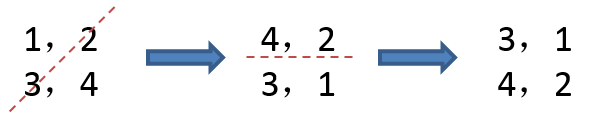
\includegraphics[width=200pt]{rotate-image.png}\\
	\figcaption{Rotate Image}\label{fig:rotate-image}
\end{center}

或者,首先沿着水平中线翻转一次,然后沿着主对角线翻转一次。


\subsubsection{代码1}
\begin{Code}
	// LeetCode, Rotate Image
	// 思路 1,时间复杂度O(n^2),空间复杂度O(1)
	class Solution {
		public:
		void rotate(vector<vector<int>>& matrix) {
			const int n = matrix.size();
			
			for (int i = 0; i < n; ++i)  // 沿着副对角线反转
			for (int j = 0; j < n - i; ++j)
			swap(matrix[i][j], matrix[n - 1 - j][n - 1 - i]);
			
			for (int i = 0; i < n / 2; ++i) // 沿着水平中线反转
			for (int j = 0; j < n; ++j)
			swap(matrix[i][j], matrix[n - 1 - i][j]);
		}
	};
\end{Code}

\subsubsection{代码2}
\begin{Code}
	// LeetCode, Rotate Image
	// 思路 2,时间复杂度O(n^2),空间复杂度O(1)
	class Solution {
		public:
		void rotate(vector<vector<int>>& matrix) {
			const int n = matrix.size();
			
			for (int i = 0; i < n / 2; ++i) // 沿着水平中线反转
			for (int j = 0; j < n; ++j)
			swap(matrix[i][j], matrix[n - 1 - i][j]);
			
			for (int i = 0; i < n; ++i)  // 沿着主对角线反转
			for (int j = i + 1; j < n; ++j)
			swap(matrix[i][j], matrix[j][i]);
		}
	};
\end{Code}


\subsubsection{相关题目}
\begindot
\item 无
\myenddot


\subsection{Plus One} %%%%%%%%%%%%%%%%%%%%%%%%%%%%%%
\label{sec:plus-one}


\subsubsection{描述}
Given a number represented as an array of digits, plus one to the number.


\subsubsection{分析}
高精度加法。


\subsubsection{代码1}
\begin{Code}
	// LeetCode, Plus One
	// 时间复杂度O(n),空间复杂度O(1)
	class Solution {
		public:
		vector<int> plusOne(vector<int> &digits) {
			add(digits, 1);
			return digits;
		}
		private:
		// 0 <= digit <= 9
		void add(vector<int> &digits, int digit) {
			int c = digit;  // carry, 进位
			
			for (auto it = digits.rbegin(); it != digits.rend(); ++it) {
				*it += c;
				c = *it / 10;
				*it %= 10;
			}
			
			if (c > 0) digits.insert(digits.begin(), 1);
		}
	};
\end{Code}


\subsubsection{代码2}
\begin{Code}
	// LeetCode, Plus One
	// 时间复杂度O(n),空间复杂度O(1)
	class Solution {
		public:
		vector<int> plusOne(vector<int> &digits) {
			add(digits, 1);
			return digits;
		}
		private:
		// 0 <= digit <= 9
		void add(vector<int> &digits, int digit) {
			int c = digit;  // carry, 进位
			
			for_each(digits.rbegin(), digits.rend(), [&c](int &d){
				d += c;
				c = d / 10;
				d %= 10;
			});
			
			if (c > 0) digits.insert(digits.begin(), 1);
		}
	};
\end{Code}


\subsubsection{相关题目}
\begindot
\item 无
\myenddot


\subsection{Climbing Stairs} %%%%%%%%%%%%%%%%%%%%%%%%%%%%%%
\label{sec:climbing-stairs}


\subsubsection{描述}
You are climbing a stair case. It takes $n$ steps to reach to the top.

Each time you can either climb 1 or 2 steps. In how many distinct ways can you 
climb to the top?


\subsubsection{分析}
设$f(n)$表示爬$n$阶楼梯的不同方法数,为了爬到第$n$阶楼梯,有两个选择:
\begindot
\item 从第$n-1$阶前进1步;
\item 从第$n-1$阶前进2步;
\myenddot
因此,有$f(n)=f(n-1)+f(n-2)$。

这是一个斐波那契数列。

方法1,递归,太慢;方法2,迭代。

方法3,数学公式。斐波那契数列的通项公式为 
$a_n=\dfrac{1}{\sqrt{5}}\left[\left(\dfrac{1+\sqrt{5}}{2}\right)^n-\left(\dfrac{1-\sqrt{5}}{2}\right)^n\right]$。


\subsubsection{迭代}
\begin{Code}
	// LeetCode, Climbing Stairs
	// 迭代,时间复杂度O(n),空间复杂度O(1)
	class Solution {
		public:
		int climbStairs(int n) {
			int prev = 0;
			int cur = 1;
			for(int i = 1; i <= n ; ++i){
				int tmp = cur;
				cur += prev;
				prev = tmp;
			}
			return cur;
		}
	};
\end{Code}


\subsubsection{数学公式}
\begin{Code}
	// LeetCode, Climbing Stairs
	// 数学公式,时间复杂度O(1),空间复杂度O(1)
	class Solution {
		public:
		int climbStairs(int n) {
			const double s = sqrt(5);
			return floor((pow((1+s)/2, n+1) + pow((1-s)/2, n+1))/s + 0.5);
		}
	};
\end{Code}


\subsubsection{相关题目}
\begindot
\item Decode Ways, 见 \S \ref{sec:decode-ways}
\myenddot


\subsection{Gray Code} %%%%%%%%%%%%%%%%%%%%%%%%%%%%%%
\label{sec:gray-code}


\subsubsection{描述}
The gray code is a binary numeral system where two successive values differ in 
only one bit.

Given a non-negative integer $n$ representing the total number of bits in the 
code, print the sequence of gray code. A gray code sequence must begin with 0.

For example, given $n = 2$, return \fn{[0,1,3,2]}. Its gray code sequence is:
\begin{Code}
	00 - 0
	01 - 1
	11 - 3
	10 - 2
\end{Code}

Note:
\begindot
\item For a given $n$, a gray code sequence is not uniquely defined.
\item For example, \fn{[0,2,3,1]} is also a valid gray code sequence according 
to the above definition.
\item For now, the judge is able to judge based on one instance of gray code 
sequence. Sorry about that.
\myenddot


\subsubsection{分析}
格雷码(Gray Code)的定义请参考 \myurl{http://en.wikipedia.org/wiki/Gray_code}

\textbf{自然二进制码转换为格雷码:$g_0=b_0, g_i=b_i \oplus b_{i-1}$}

保留自然二进制码的最高位作为格雷码的最高位,格雷码次高位为二进制码的高位与次高位异或,其余各位与次高位的求法类似。例如,将自然二进制码1001,转换为格雷码的过程是:保留最高位;然后将第1位的1和第2位的0异或,得到1,作为格雷码的第2位;将第2位的0和第3位的0异或,得到0,作为格雷码的第3位;将第3位的0和第4位的1异或,得到1,作为格雷码的第4位,最终,格雷码为1101。

\textbf{格雷码转换为自然二进制码:$b_0=g_0, b_i=g_i \oplus b_{i-1}$}

保留格雷码的最高位作为自然二进制码的最高位,次高位为自然二进制高位与格雷码次高位异或,其余各位与次高位的求法类似。例如,将格雷码1000转换为自然二进制码的过程是:保留最高位1,作为自然二进制码的最高位;然后将自然二进制码的第1位1和格雷码的第2位0异或,得到1,作为自然二进制码的第2位;将自然二进制码的第2位1和格雷码的第3位0异或,得到1,作为自然二进制码的第3位;将自然二进制码的第3位1和格雷码的第4位0异或,得到1,作为自然二进制码的第4位,最终,自然二进制码为1111。

格雷码有\textbf{数学公式},整数$n$的格雷码是$n \oplus (n/2)$。

这题要求生成$n$比特的所有格雷码。

方法1,最简单的方法,利用数学公式,对从 $0\sim2^n-1$的所有整数,转化为格雷码。

方法2,$n$比特的格雷码,可以递归地从$n-1$比特的格雷码生成。如图\S 
\ref{fig:gray-code-construction}所示。

\begin{center}
	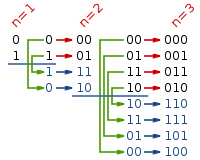
\includegraphics[width=160pt]{gray-code-construction.png}\\
	\figcaption{The first few steps of the reflect-and-prefix 
	method.}\label{fig:gray-code-construction}
\end{center}


\subsubsection{数学公式}
\begin{Code}
	// LeetCode, Gray Code
	// 数学公式,时间复杂度O(2^n),空间复杂度O(1)
	class Solution {
		public:
		vector<int> grayCode(int n) {
			vector<int> result;
			const size_t size = 1 << n;  // 2^n
			result.reserve(size);
			for (size_t i = 0; i < size; ++i)
			result.push_back(binary_to_gray(i));
			return result;
		}
		private:
		static unsigned int binary_to_gray(unsigned int n) {
			return n ^ (n >> 1);
		}
	};
\end{Code}


\subsubsection{Reflect-and-prefix method}
\begin{Code}
	// LeetCode, Gray Code
	// reflect-and-prefix method
	// 时间复杂度O(2^n),空间复杂度O(1)
	class Solution {
		public:
		vector<int> grayCode(int n) {
			vector<int> result;
			result.reserve(1<<n);
			result.push_back(0);
			for (int i = 0; i < n; i++) {
				const int highest_bit = 1 << i;
				for (int j = result.size() - 1; j >= 0; j--) // 要反着遍历,才能对称
				result.push_back(highest_bit | result[j]);
			}
			return result;
		}
	};
\end{Code}


\subsubsection{相关题目}
\begindot
\item 无
\myenddot


\subsection{Set Matrix Zeroes} %%%%%%%%%%%%%%%%%%%%%%%%%%%%%%
\label{sec:set-matrix-zeroes}


\subsubsection{描述}
Given a $m \times n$ matrix, if an element is 0, set its entire row and column 
to 0. Do it in place.

\textbf{Follow up:}
Did you use extra space?

A straight forward solution using $O(mn)$ space is probably a bad idea.

A simple improvement uses $O(m + n)$ space, but still not the best solution.

Could you devise a constant space solution?


\subsubsection{分析}
$O(m+n)$空间的方法很简单,设置两个bool数组,记录每行和每列是否存在0。

想要常数空间,可以复用第一行和第一列。


\subsubsection{代码1}
\begin{Code}
	// LeetCode, Set Matrix Zeroes
	// 时间复杂度O(m*n),空间复杂度O(m+n)
	class Solution {
		public:
		void setZeroes(vector<vector<int> > &matrix) {
			const size_t m = matrix.size();
			const size_t n = matrix[0].size();
			vector<bool> row(m, false); // 标记该行是否存在0
			vector<bool> col(n, false); // 标记该列是否存在0
			
			for (size_t i = 0; i < m; ++i) {
				for (size_t j = 0; j < n; ++j) {
					if (matrix[i][j] == 0) {
						row[i] = col[j] = true;
					}
				}
			}
			
			for (size_t i = 0; i < m; ++i) {
				if (row[i])
				fill(&matrix[i][0], &matrix[i][0] + n, 0);
			}
			for (size_t j = 0; j < n; ++j) {
				if (col[j]) {
					for (size_t i = 0; i < m; ++i) {
						matrix[i][j] = 0;
					}
				}
			}
		}
	};
\end{Code}


\subsubsection{代码2}
\begin{Code}
	// LeetCode, Set Matrix Zeroes
	// 时间复杂度O(m*n),空间复杂度O(1)
	class Solution {
		public:
		void setZeroes(vector<vector<int> > &matrix) {
			const size_t m = matrix.size();
			const size_t n = matrix[0].size();
			bool row_has_zero = false; // 第一行是否存在 0
			bool col_has_zero = false; // 第一列是否存在 0
			
			for (size_t i = 0; i < n; i++)
			if (matrix[0][i] == 0) {
				row_has_zero = true;
				break;
			}
			
			for (size_t i = 0; i < m; i++)
			if (matrix[i][0] == 0) {
				col_has_zero = true;
				break;
			}
			
			for (size_t i = 1; i < m; i++)
			for (size_t j = 1; j < n; j++)
			if (matrix[i][j] == 0) {
				matrix[0][j] = 0;
				matrix[i][0] = 0;
			}
			for (size_t i = 1; i < m; i++)
			for (size_t j = 1; j < n; j++)
			if (matrix[i][0] == 0 || matrix[0][j] == 0)
			matrix[i][j] = 0;
			if (row_has_zero)
			for (size_t i = 0; i < n; i++)
			matrix[0][i] = 0;
			if (col_has_zero)
			for (size_t i = 0; i < m; i++)
			matrix[i][0] = 0;
		}
	};
\end{Code}


\subsubsection{相关题目}
\begindot
\item 无
\myenddot


\subsection{Gas Station} %%%%%%%%%%%%%%%%%%%%%%%%%%%%%%
\label{sec:gas-station}


\subsubsection{描述}
There are $N$ gas stations along a circular route, where the amount of gas at 
station $i$ is \fn{gas[i]}.

You have a car with an unlimited gas tank and it costs \fn{cost[i]} of gas to 
travel from station $i$ to its next station ($i$+1). You begin the journey with 
an empty tank at one of the gas stations.

Return the starting gas station's index if you can travel around the circuit 
once, otherwise return -1.

Note:
The solution is guaranteed to be unique.


\subsubsection{分析}
首先想到的是$O(N^2)$的解法,对每个点进行模拟。

$O(N)$的解法是,设置两个变量,\fn{sum}判断当前的指针的有效性;\fn{total}则判断整个数组是否有解,有就返回通过\fn{sum}得到的下标,没有则返回-1。


\subsubsection{代码}
\begin{Code}
	// LeetCode, Gas Station
	// 时间复杂度O(n),空间复杂度O(1)
	class Solution {
		public:
		int canCompleteCircuit(vector<int> &gas, vector<int> &cost) {
			int total = 0;
			int j = -1;
			for (int i = 0, sum = 0; i < gas.size(); ++i) {
				sum += gas[i] - cost[i];
				total += gas[i] - cost[i];
				if (sum < 0) {
					j = i;
					sum = 0;
				}
			}
			return total >= 0 ? j + 1 : -1;
		}
	};
\end{Code}


\subsubsection{相关题目}
\begindot
\item 无
\myenddot


\subsection{Candy} %%%%%%%%%%%%%%%%%%%%%%%%%%%%%%
\label{sec:candy}


\subsubsection{描述}
There are $N$ children standing in a line. Each child is assigned a rating 
value.

You are giving candies to these children subjected to the following 
requirements:
\begindot
\item Each child must have at least one candy.
\item Children with a higher rating get more candies than their neighbors.
\myenddot

What is the minimum candies you must give?


\subsubsection{分析}
无


\subsubsection{迭代版}
\begin{Code}
	// LeetCode, Candy
	// 时间复杂度O(n),空间复杂度O(n)
	class Solution {
		public:
		int candy(vector<int> &ratings) {
			const int n = ratings.size();
			vector<int> increment(n);
			
			// 左右各扫描一遍
			for (int i = 1, inc = 1; i < n; i++) {
				if (ratings[i] > ratings[i - 1])
				increment[i] = max(inc++, increment[i]);
				else
				inc = 1;
			}
			
			for (int i = n - 2, inc = 1; i >= 0; i--) {
				if (ratings[i] > ratings[i + 1])
				increment[i] = max(inc++, increment[i]);
				else
				inc = 1;
			}
			// 初始值为n,因为每个小朋友至少一颗糖
			return accumulate(&increment[0], &increment[0]+n, n);
		}
	};
\end{Code}


\subsubsection{递归版}
\begin{Code}
	// LeetCode, Candy
	// 备忘录法,时间复杂度O(n),空间复杂度O(n)
	// @author fancymouse (http://weibo.com/u/1928162822)
	class Solution {
		public:
		int candy(const vector<int>& ratings) {
			vector<int> f(ratings.size());
			int sum = 0;
			for (int i = 0; i < ratings.size(); ++i)
			sum += solve(ratings, f, i);
			return sum;
		}
		int solve(const vector<int>& ratings, vector<int>& f, int i) {
			if (f[i] == 0) {
				f[i] = 1;
				if (i > 0 && ratings[i] > ratings[i - 1])
				f[i] = max(f[i], solve(ratings, f, i - 1) + 1);
				if (i < ratings.size() - 1 && ratings[i] > ratings[i + 1])
				f[i] = max(f[i], solve(ratings, f, i + 1) + 1);
			}
			return f[i];
		}
	};
\end{Code}


\subsubsection{相关题目}
\begindot
\item 无
\myenddot


\subsection{Single Number} %%%%%%%%%%%%%%%%%%%%%%%%%%%%%%
\label{sec:single-number}


\subsubsection{描述}
Given an array of integers, every element appears twice except for one. Find 
that single one.

Note:
Your algorithm should have a linear runtime complexity. Could you implement it 
without using extra memory?


\subsubsection{分析}
异或,不仅能处理两次的情况,只要出现偶数次,都可以清零。


\subsubsection{代码1}
\begin{Code}
	// LeetCode, Single Number
	// 时间复杂度O(n),空间复杂度O(1)
	class Solution {
		public:
		int singleNumber(int A[], int n) {
			int x = 0;
			for (size_t i = 0; i < n; ++i)
			x ^= A[i];
			return x;
		}
	};
\end{Code}


\subsubsection{代码2}
\begin{Code}
	// LeetCode, Single Number
	// 时间复杂度O(n),空间复杂度O(1)
	class Solution {
		public:
		int singleNumber(int A[], int n) {
			return accumulate(A, A + n, 0, bit_xor<int>());
		}
	};
\end{Code}


\subsubsection{相关题目}
\begindot
\item  Single Number II, 见 \S \ref{sec:single-number-ii}
\myenddot


\subsection{Single Number II} %%%%%%%%%%%%%%%%%%%%%%%%%%%%%%
\label{sec:single-number-ii}


\subsubsection{描述}
Given an array of integers, every element appears three times except for one. 
Find that single one.

Note:
Your algorithm should have a linear runtime complexity. Could you implement it 
without using extra memory?


\subsubsection{分析}
本题和上一题 Single Number,考察的是位运算。

方法1:创建一个长度为\fn{sizeof(int)}的数组\fn{count[sizeof(int)]},\fn{count[i]}表示在在$i$位出现的1的次数。如果\fn{count[i]}是3的整数倍,则忽略;否则就把该位取出来组成答案。

方法2:用\fn{one}记录到当前处理的元素为止,二进制1出现“1次”(mod 3 之后的 
1)的有哪些二进制位;用\fn{two}记录到当前计算的变量为止,二进制1出现“2次”(mod 3 之后的 
2)的有哪些二进制位。当\fn{one}和\fn{two}中的某一位同时为1时表示该二进制位上1出现了3次,此时需要清零。即\textbf{用二进制模拟三进制运算}。最终\fn{one}记录的是最终结果。

\subsubsection{代码1}
\begin{Code}
	// LeetCode, Single Number II
	// 方法1,时间复杂度O(n),空间复杂度O(1)
	class Solution {
		public:
		int singleNumber(int A[], int n) {
			const int W = sizeof(int) * 8; // 一个整数的bit数,即整数字长
			int count[W];  // count[i]表示在在i位出现的1的次数
			fill_n(&count[0], W, 0);
			for (int i = 0; i < n; i++) {
				for (int j = 0; j < W; j++) {
					count[j] += (A[i] >> j) & 1;
					count[j] %= 3;
				}
			}
			int result = 0;
			for (int i = 0; i < W; i++) {
				result += (count[i] << i);
			}
			return result;
		}
	};
\end{Code}


\subsubsection{代码2}
\begin{Code}
	// LeetCode, Single Number II
	// 方法2,时间复杂度O(n),空间复杂度O(1)
	class Solution {
		public:
		int singleNumber(int A[], int n) {
			int one = 0, two = 0, three = 0;
			for (int i = 0; i < n; ++i) {
				two |= (one & A[i]);
				one ^= A[i];
				three = ~(one & two);
				one &= three;
				two &= three;
			}
			
			return one;
		}
	};
\end{Code}


\subsubsection{相关题目}
\begindot
\item  Single Number, 见 \S \ref{sec:single-number}
\myenddot

\subsection{Vector Class}
\subsubsection{描述}
Implement a vector-like data structure from scratch. 

This question was to be done in C or C++. 

Discussion topics: 
1. Dealing with out of bounds accesses. 
2. What happens when you need to increase the vector's size? 
3. How many copies does the structure perform to insert n elements? That is, n 
calls to vector.push_back

\subsection{N Parking Slots for N-1 Cars Sorting}
\subsubsection{描述}
There are N parking slots and N-1 cars. Everytime you can move one car. How to move these cars into one given order. 
BTW: I got this question from internet but i could not figure it out partially because the description is kind of incomplete to me. Anyone knowing this question or the solution?
\subsubsection{分析}
Sorting with O(1) space, e.g., insertsorting, selectsorting



\section{单链表} %%%%%%%%%%%%%%%%%%%%%%%%%%%%%%

单链表节点的定义如下:
\begin{Code}
	// 单链表节点
	struct ListNode {
		int val;
		ListNode *next;
		ListNode(int x) : val(x), next(nullptr) { }
	};
\end{Code}


\subsection{Add Two Numbers}
\label{sec:add-two-numbers}


\subsubsection{描述}
You are given two linked lists representing two non-negative numbers. The 
digits are stored in reverse order and each of their nodes contain a single 
digit. Add the two numbers and return it as a linked list.

Input: {\small \fontspec{Latin Modern Mono} (2 -> 4 -> 3) + (5 -> 6 -> 4)}

Output: {\small \fontspec{Latin Modern Mono} 7 -> 0 -> 8}


\subsubsection{分析}
跟Add Binary(见 \S \ref{sec:add-binary})很类似


\subsubsection{代码}
\begin{Code}
	// LeetCode, Add Two Numbers
	// 跟Add Binary 很类似
	// 时间复杂度O(m+n),空间复杂度O(1)
	class Solution {
		public:
		ListNode *addTwoNumbers(ListNode *l1, ListNode *l2) {
			ListNode dummy(-1); // 头节点
			int carry = 0;
			ListNode *prev = &dummy;
			for (ListNode *pa = l1, *pb = l2;
			pa != nullptr || pb != nullptr;
			pa = pa == nullptr ? nullptr : pa->next,
			pb = pb == nullptr ? nullptr : pb->next,
			prev = prev->next) {
				const int ai = pa == nullptr ? 0 : pa->val;
				const int bi = pb == nullptr ? 0 : pb->val;
				const int value = (ai + bi + carry) % 10;
				carry = (ai + bi + carry) / 10;
				prev->next = new ListNode(value); // 尾插法
			}
			if (carry > 0)
			prev->next = new ListNode(carry);
			return dummy.next;
		}
	};
\end{Code}


\subsubsection{相关题目}

\begindot
\item Add Binary, 见 \S \ref{sec:add-binary}
\myenddot


\subsection{Reverse Linked List II}
\label{sec:reverse-linked-list-ii}


\subsubsection{描述}
Reverse a linked list from position $m$ to $n$. Do it in-place and in one-pass.

For example:
Given \code{1->2->3->4->5->nullptr}, $m$ = 2 and $n$ = 4,

return \code{1->4->3->2->5->nullptr}.

Note:
Given m, n satisfy the following condition:
$1 \leq m \leq  n \leq $ length of list.


\subsubsection{分析}
这题非常繁琐,有很多边界检查,15分钟内做到bug free很有难度!


\subsubsection{代码}
\begin{Code}
	// LeetCode, Reverse Linked List II
	// 迭代版,时间复杂度O(n),空间复杂度O(1)
	class Solution {
		public:
		ListNode *reverseBetween(ListNode *head, int m, int n) {
			ListNode dummy(-1);
			dummy.next = head;
			
			ListNode *prev = &dummy;
			for (int i = 0; i < m-1; ++i)
			prev = prev->next;
			ListNode* const head2 = prev;
			
			prev = head2->next;
			ListNode *cur = prev->next;
			for (int i = m; i < n; ++i) {
				prev->next = cur->next;
				cur->next = head2->next;
				head2->next = cur;  // 头插法
				cur = prev->next;
			}
			
			return dummy.next;
		}
	};
\end{Code}


\subsubsection{相关题目}

\begindot
\item 无
\myenddot


\subsection{Partition List}
\label{sec:partition-list}


\subsubsection{描述}
Given a linked list and a value $x$, partition it such that all nodes less than 
$x$ come before nodes greater than or equal to $x$.

You should preserve the original relative order of the nodes in each of the two 
partitions.

For example,
Given \code{1->4->3->2->5->2} and \code{x = 3}, return \code{1->2->2->4->3->5}.


\subsubsection{分析}
无


\subsubsection{代码}
\begin{Code}
	// LeetCode, Partition List
	// 时间复杂度O(n),空间复杂度O(1)
	class Solution {
		public:
		ListNode* partition(ListNode* head, int x) {
			ListNode left_dummy(-1); // 头结点
			ListNode right_dummy(-1); // 头结点
			
			auto left_cur = &left_dummy;
			auto right_cur = &right_dummy;
			
			for (ListNode *cur = head; cur; cur = cur->next) {
				if (cur->val < x) {
					left_cur->next = cur;
					left_cur = cur;
				} else {
				right_cur->next = cur;
				right_cur = cur;
			}
		}
		
		left_cur->next = right_dummy.next;
		right_cur->next = nullptr;
		
		return left_dummy.next;
	}
};
\end{Code}


\subsubsection{相关题目}

\begindot
\item 无
\myenddot


\subsection{Remove Duplicates from Sorted List}
\label{sec:remove-duplicates-from-sorted-list}


\subsubsection{描述}
Given a sorted linked list, delete all duplicates such that each element appear 
only once.

For example,

Given \code{1->1->2}, return \code{1->2}.

Given \code{1->1->2->3->3}, return \code{1->2->3}.


\subsubsection{分析}
无


\subsubsection{递归版}
\begin{Code}
	// LeetCode, Remove Duplicates from Sorted List
	// 递归版,时间复杂度O(n),空间复杂度O(1)
	class Solution {
		public:
		ListNode *deleteDuplicates(ListNode *head) {
			if (!head) return head;
			ListNode dummy(head->val + 1); // 值只要跟head不同即可
			dummy.next = head;
			
			recur(&dummy, head);
			return dummy.next;
		}
		private:
		static void recur(ListNode *prev, ListNode *cur) {
			if (cur == nullptr) return;
			
			if (prev->val == cur->val) { // 删除head
				prev->next = cur->next;
				delete cur;
				recur(prev, prev->next);
			} else {
			recur(prev->next, cur->next);
		}
	}
};
\end{Code}


\subsubsection{迭代版}
\begin{Code}
	// LeetCode, Remove Duplicates from Sorted List
	// 迭代版,时间复杂度O(n),空间复杂度O(1)
	class Solution {
		public:
		ListNode *deleteDuplicates(ListNode *head) {
			if (head == nullptr) return nullptr;
			
			for (ListNode *prev = head, *cur = head->next; cur; cur = 
			cur->next) {
				if (prev->val == cur->val) {
					prev->next = cur->next;
					delete cur;
				} else {
				prev = cur;
			}
		}
		return head;
	}
};
\end{Code}


\subsubsection{相关题目}

\begindot
\item Remove Duplicates from Sorted List II,见 \S 
\ref{sec:remove-duplicates-from-sorted-list-ii}
\myenddot


\subsection{Remove Duplicates from Sorted List II}
\label{sec:remove-duplicates-from-sorted-list-ii}


\subsubsection{描述}
Given a sorted linked list, delete all nodes that have duplicate numbers, 
leaving only distinct numbers from the original list.

For example,

Given \code{1->2->3->3->4->4->5}, return \code{1->2->5}.

Given \code{1->1->1->2->3}, return \code{2->3}.


\subsubsection{分析}
无


\subsubsection{递归版}
\begin{Code}
	// LeetCode, Remove Duplicates from Sorted List II
	// 递归版,时间复杂度O(n),空间复杂度O(1)
	class Solution {
		public:
		ListNode *deleteDuplicates(ListNode *head) {
			if (!head || !head->next) return head;
			
			ListNode *p = head->next;
			if (head->val == p->val) {
				while (p && head->val == p->val) {
					ListNode *tmp = p;
					p = p->next;
					delete tmp;
				}
				delete head;
				return deleteDuplicates(p);
			} else {
			head->next = deleteDuplicates(head->next);
			return head;
		}
	}
};
\end{Code}


\subsubsection{迭代版}
\begin{Code}
	// LeetCode, Remove Duplicates from Sorted List II
	// 迭代版,时间复杂度O(n),空间复杂度O(1)
	class Solution {
		public:
		ListNode *deleteDuplicates(ListNode *head) {
			if (head == nullptr) return head;
			
			ListNode dummy(INT_MIN); // 头结点
			dummy.next = head;
			ListNode *prev = &dummy, *cur = head;
			while (cur != nullptr) {
				bool duplicated = false;
				while (cur->next != nullptr && cur->val == cur->next->val) {
					duplicated = true;
					ListNode *temp = cur;
					cur = cur->next;
					delete temp;
				}
				if (duplicated) { // 删除重复的最后一个元素
					ListNode *temp = cur;
					cur = cur->next;
					delete temp;
					continue;
				}
				prev->next = cur;
				prev = prev->next;
				cur = cur->next;
			}
			prev->next = cur;
			return dummy.next;
		}
	};
\end{Code}


\subsubsection{相关题目}

\begindot
\item Remove Duplicates from Sorted List,见 \S 
\ref{sec:remove-duplicates-from-sorted-list}
\myenddot


\subsection{Rotate List}
\label{sec:rotate-list}


\subsubsection{描述}
Given a list, rotate the list to the right by $k$ places, where $k$ is 
non-negative.

For example:
Given \code{1->2->3->4->5->nullptr} and \code{k = 2}, return 
\code{4->5->1->2->3->nullptr}.


\subsubsection{分析}
先遍历一遍,得出链表长度$len$,注意$k$可能大于$len$,因此令$k \%= 
len$。将尾节点next指针指向首节点,形成一个环,接着往后跑$len-k$步,从这里断开,就是要求的结果了。


\subsubsection{代码}
\begin{Code}
	// LeetCode, Remove Rotate List
	// 时间复杂度O(n),空间复杂度O(1)
	class Solution {
		public:
		ListNode *rotateRight(ListNode *head, int k) {
			if (head == nullptr || k == 0) return head;
			
			int len = 1;
			ListNode* p = head;
			while (p->next) { // 求长度
				len++;
				p = p->next;
			}
			k = len - k % len;
			
			p->next = head; // 首尾相连
			for(int step = 0; step < k; step++) {
				p = p->next;  //接着往后跑
			}
			head = p->next; // 新的首节点
			p->next = nullptr; // 断开环
			return head;
		}
	};
\end{Code}


\subsubsection{相关题目}

\begindot
\item 无
\myenddot


\subsection{Remove Nth Node From End of List}
\label{sec:remove-nth-node-from-end-of-list}


\subsubsection{描述}
Given a linked list, remove the $n^{th}$ node from the end of list and return 
its head.

For example, Given linked list: \code{1->2->3->4->5}, and $n$ = 2.

After removing the second node from the end, the linked list becomes 
\code{1->2->3->5}.

Note:
\begindot
\item Given $n$ will always be valid.
\item Try to do this in one pass.
\myenddot


\subsubsection{分析}
设两个指针$p,q$,让$q$先走$n$步,然后$p$和$q$一起走,直到$q$走到尾节点,删除\fn{p->next}即可。


\subsubsection{代码}
\begin{Code}
	// LeetCode, Remove Nth Node From End of List
	// 时间复杂度O(n),空间复杂度O(1)
	class Solution {
		public:
		ListNode *removeNthFromEnd(ListNode *head, int n) {
			ListNode dummy{-1, head};
			ListNode *p = &dummy, *q = &dummy;
			
			for (int i = 0; i < n; i++)  // q先走n步
			q = q->next;
			
			while(q->next) { // 一起走
				p = p->next;
				q = q->next;
			}
			ListNode *tmp = p->next;
			p->next = p->next->next;
			delete tmp;
			return dummy.next;
		}
	};
\end{Code}


\subsubsection{相关题目}

\begindot
\item 无
\myenddot


\subsection{Swap Nodes in Pairs}
\label{sec:swap-nodes-in-pairs}


\subsubsection{描述}
Given a linked list, swap every two adjacent nodes and return its head.

For example,
Given \code{1->2->3->4}, you should return the list as \code{2->1->4->3}.

Your algorithm should use only constant space. You may \emph{not} modify the 
values in the list, only nodes itself can be changed.


\subsubsection{分析}
无


\subsubsection{代码}
\begin{Code}
	// LeetCode, Swap Nodes in Pairs
	// 时间复杂度O(n),空间复杂度O(1)
	class Solution {
		public:
		ListNode *swapPairs(ListNode *head) {
			if (head == nullptr || head->next == nullptr) return head;
			ListNode dummy(-1);
			dummy.next = head;
			
			for(ListNode *prev = &dummy, *cur = prev->next, *next = cur->next;
			next;
			prev = cur, cur = cur->next, next = cur ? cur->next: nullptr) {
				prev->next = next;
				cur->next = next->next;
				next->next = cur;
			}
			return dummy.next;
		}
	};
\end{Code}

下面这种写法更简洁,但题目规定了不准这样做。
\begin{Code}
	// LeetCode, Swap Nodes in Pairs
	// 时间复杂度O(n),空间复杂度O(1)
	class Solution {
		public:
		ListNode* swapPairs(ListNode* head) {
			ListNode* p = head;
			
			while (p && p->next) {
				swap(p->val, p->next->val);
				p = p->next->next;
			}
			
			return head;
		}
	};
\end{Code}

\subsubsection{相关题目}

\begindot
\item Reverse Nodes in k-Group, 见 \S \ref{sec:reverse-nodes-in-k-group}
\myenddot


\subsection{Reverse Nodes in k-Group}
\label{sec:reverse-nodes-in-k-group}


\subsubsection{描述}
Given a linked list, reverse the nodes of a linked list k at a time and return 
its modified list.

If the number of nodes is not a multiple of $k$ then left-out nodes in the end 
should remain as it is.

You may not alter the values in the nodes, only nodes itself may be changed.

Only constant memory is allowed.

For example,
Given this linked list: \code{1->2->3->4->5}

For $k = 2$, you should return: \code{2->1->4->3->5}

For $k = 3$, you should return: \code{3->2->1->4->5}


\subsubsection{分析}
无


\subsubsection{递归版}
\begin{Code}
	// LeetCode, Reverse Nodes in k-Group
	// 递归版,时间复杂度O(n),空间复杂度O(1)
	class Solution {
		public:
		ListNode *reverseKGroup(ListNode *head, int k) {
			if (head == nullptr || head->next == nullptr || k < 2)
			return head;
			
			ListNode *next_group = head;
			for (int i = 0; i < k; ++i) {
				if (next_group)
				next_group = next_group->next;
				else
				return head;
			}
			// next_group is the head of next group
			// new_next_group is the new head of next group after reversion
			ListNode *new_next_group = reverseKGroup(next_group, k);
			ListNode *prev = NULL, *cur = head;
			while (cur != next_group) {
				ListNode *next = cur->next;
				cur->next = prev ? prev : new_next_group;
				prev = cur;
				cur = next;
			}
			return prev; // prev will be the new head of this group
		}
	};
\end{Code}


\subsubsection{迭代版}
\begin{Code}
	// LeetCode, Reverse Nodes in k-Group
	// 迭代版,时间复杂度O(n),空间复杂度O(1)
	class Solution {
		public:
		ListNode *reverseKGroup(ListNode *head, int k) {
			if (head == nullptr || head->next == nullptr || k < 2) return head;
			ListNode dummy(-1);
			dummy.next = head;
			
			for(ListNode *prev = &dummy, *end = head; end; end = prev->next) {
				for (int i = 1; i < k && end; i++)
				end = end->next;
				if (end  == nullptr) break;  // 不足 k 个
				
				prev = reverse(prev, prev->next, end);
			}
			
			return dummy.next;
		}
		
		// prev 是 first 前一个元素, [begin, end] 闭区间,保证三者都不为 null
		// 返回反转后的倒数第1个元素
		ListNode* reverse(ListNode *prev, ListNode *begin, ListNode *end) {
			ListNode *end_next = end->next;
			for (ListNode *p = begin, *cur = p->next, *next = cur->next;
			cur != end_next;
			p = cur, cur = next, next = next ? next->next : nullptr) {
				cur->next = p;
			}
			begin->next = end_next;
			prev->next = end;
			return begin;
		}
	};
\end{Code}


\subsubsection{相关题目}
\begindot
\item Swap Nodes in Pairs, 见 \S \ref{sec:swap-nodes-in-pairs}
\myenddot


\subsection{Copy List with Random Pointer}
\label{sec:copy-list-with-random-pointer}


\subsubsection{描述}
A linked list is given such that each node contains an additional random 
pointer which could point to any node in the list or null.

Return a deep copy of the list.


\subsubsection{分析}
无


\subsubsection{代码}
\begin{Code}
	// LeetCode, Copy List with Random Pointer
	// 两遍扫描,时间复杂度O(n),空间复杂度O(1)
	class Solution {
		public:
		RandomListNode *copyRandomList(RandomListNode *head) {
			for (RandomListNode* cur = head; cur != nullptr; ) {
				RandomListNode* node = new RandomListNode(cur->label);
				node->next = cur->next;
				cur->next = node;
				cur = node->next;
			}
			
			for (RandomListNode* cur = head; cur != nullptr; ) {
				if (cur->random != NULL)
				cur->next->random = cur->random->next;
				cur = cur->next->next;
			}
			
			// 分拆两个单链表
			RandomListNode dummy(-1);
			for (RandomListNode* cur = head, *new_cur = &dummy;
			cur != nullptr; ) {
				new_cur->next = cur->next;
				new_cur = new_cur->next;
				cur->next = cur->next->next;
				cur = cur->next;
			}
			return dummy.next;
		}
	};
\end{Code}


\subsubsection{相关题目}
\begindot
\item 无
\myenddot


\subsection{Linked List Cycle}
\label{sec:Linked-List-Cycle}


\subsubsection{描述}
Given a linked list, determine if it has a cycle in it.
Follow up:
Can you solve it without using extra space?


\subsubsection{分析}
最容易想到的方法是,用一个哈希表\fn{unordered_map<int, bool> 
visited},记录每个元素是否被访问过,一旦出现某个元素被重复访问,说明存在环。空间复杂度$O(n)$,时间复杂度$O(N)$。

最好的方法是时间复杂度$O(n)$,空间复杂度$O(1)$的。设置两个指针,一个快一个慢,快的指针每次走两步,慢的指针每次走一步,如果快指针和慢指针相遇,则说明有环。参考\myurl{
 http://leetcode.com/2010/09/detecting-loop-in-singly-linked-list.html}


\subsubsection{代码}
\begin{Code}
	//LeetCode, Linked List Cycle
	// 时间复杂度O(n),空间复杂度O(1)
	class Solution {
		public:
		bool hasCycle(ListNode *head) {
			// 设置两个指针,一个快一个慢
			ListNode *slow = head, *fast = head;
			while (fast && fast->next) {
				slow = slow->next;
				fast = fast->next->next;
				if (slow == fast) return true;
			}
			return false;
		}
	};
\end{Code}


\subsubsection{相关题目}
\begindot
\item Linked List Cycle II, 见 \S \ref{sec:Linked-List-Cycle-II}
\myenddot


\subsection{Linked List Cycle II}
\label{sec:Linked-List-Cycle-II}

\subsubsection{描述}
Given a linked list, return the node where the cycle begins. If there is no 
cycle, return \fn{null}.
Follow up:
Can you solve it without using extra space?

\subsubsection{分析}
当fast与slow相遇时,slow肯定没有遍历完链表,而fast已经在环内循环了$n$圈($1 \leq 
n$)。假设slow走了$s$步,则fast走了$2s$步(fast步数还等于$s$加上在环上多转的$n$圈),设环长为$r$,则:
\begin{eqnarray}
	2s &=& s + nr \nonumber \\
	s &=& nr \nonumber
\end{eqnarray}

设整个链表长$L$,环入口点与相遇点距离为$a$,起点到环入口点的距离为$x$,则
\begin{eqnarray}
	x + a &=& nr = (n – 1)r +r = (n-1)r + L - x \nonumber \\
	x &=& (n-1)r + (L – x – a) \nonumber
\end{eqnarray}

$L – x – 
a$为相遇点到环入口点的距离,由此可知,从链表头到环入口点等于$n-1$圈内环+相遇点到环入口点,于是我们可以从\fn{head}开始另设一个指针\fn{slow2},两个慢指针每次前进一步,它俩一定会在环入口点相遇。

\subsubsection{代码}
\begin{Code}
	//LeetCode, Linked List Cycle II
	// 时间复杂度O(n),空间复杂度O(1)
	class Solution {
		public:
		ListNode *detectCycle(ListNode *head) {
			ListNode *slow = head, *fast = head;
			while (fast && fast->next) {
				slow = slow->next;
				fast = fast->next->next;
				if (slow == fast) {
					ListNode *slow2 = head;
					
					while (slow2 != slow) {
						slow2 = slow2->next;
						slow = slow->next;
					}
					return slow2;
				}
			}
			return nullptr;
		}
	};
\end{Code}


\subsubsection{相关题目}
\begindot
\item Linked List Cycle, 见 \S \ref{sec:Linked-List-Cycle}
\myenddot


\subsection{Reorder List}
\label{sec:Reorder-List}


\subsubsection{描述}
Given a singly linked list $L: L_0 \rightarrow L_1 \rightarrow \cdots 
\rightarrow L_{n-1} \rightarrow L_n$,
reorder it to: $L_0 \rightarrow L_n \rightarrow L_1 \rightarrow L_{n-1} 
\rightarrow L_2 \rightarrow L_{n-2} \rightarrow \cdots$

You must do this in-place without altering the nodes' values.

For example,
Given \fn{\{1,2,3,4\}}, reorder it to \fn{\{1,4,2,3\}}.


\subsubsection{分析}
题目规定要in-place,也就是说只能使用$O(1)$的空间。

可以找到中间节点,断开,把后半截单链表reverse一下,再合并两个单链表。


\subsubsection{代码}
\begin{Code}
	// LeetCode, Reorder List
	// 时间复杂度O(n),空间复杂度O(1)
	class Solution {
		public:
		void reorderList(ListNode *head) {
			if (head == nullptr || head->next == nullptr) return;
			
			ListNode *slow = head, *fast = head, *prev = nullptr;
			while (fast && fast->next) {
				prev = slow;
				slow = slow->next;
				fast = fast->next->next;
			}
			prev->next = nullptr; // cut at middle
			
			slow = reverse(slow);
			
			// merge two lists
			ListNode *curr = head;
			while (curr->next) {
				ListNode *tmp = curr->next;
				curr->next = slow;
				slow = slow->next;
				curr->next->next = tmp;
				curr = tmp;
			}
			curr->next = slow;
		}
		
		ListNode* reverse(ListNode *head) {
			if (head == nullptr || head->next == nullptr) return head;
			
			ListNode *prev = head;
			for (ListNode *curr = head->next, *next = curr->next; curr;
			prev = curr, curr = next, next = next ? next->next : nullptr) {
				curr->next = prev;
			}
			head->next = nullptr;
			return prev;
		}
	};
\end{Code}


\subsubsection{相关题目}
\begindot
\item 无
\myenddot


\subsection{LRU Cache}
\label{sec:LRU-Cachet}


\subsubsection{描述}
Design and implement a data structure for Least Recently Used (LRU) cache. It 
should support the following operations: get and set.

\fn{get(key)} - Get the value (will always be positive) of the key if the key 
exists in the cache, otherwise return -1.

\fn{set(key, value)} - Set or insert the value if the key is not already 
present. When the cache reached its capacity, it should invalidate the least 
recently used item before inserting a new item.


\subsubsection{分析}
为了使查找、插入和删除都有较高的性能,我们使用一个双向链表(\fn{std::list})和一个哈希表(\fn{std::unordered_map}),因为:
\begin{itemize}
	\item{哈希表保存每个节点的地址,可以基本保证在$O(1)$时间内查找节点}
	\item{双向链表插入和删除效率高,单向链表插入和删除时,还要查找节点的前驱节点}
\end{itemize}

具体实现细节:
\begin{itemize}
	\item{越靠近链表头部,表示节点上次访问距离现在时间最短,尾部的节点表示最近访问最少}
	\item{访问节点时,如果节点存在,把该节点交换到链表头部,同时更新hash表中该节点的地址}
	\item{插入节点时,如果cache的size达到了上限capacity,则删除尾部节点,同时要在hash表中删除对应的项;新节点插入链表头部}
	              
\end{itemize}


\subsubsection{代码}
\begin{Code}
	// LeetCode, LRU Cache
	// 时间复杂度O(logn),空间复杂度O(n)
	class LRUCache{
		private:
		struct CacheNode {
			int key;
			int value;
			CacheNode(int k, int v) :key(k), value(v){}
		};
		public:
		LRUCache(int capacity) {
			this->capacity = capacity;
		}
		
		int get(int key) {
			if (cacheMap.find(key) == cacheMap.end()) return -1;
			
			// 把当前访问的节点移到链表头部,并且更新map中该节点的地址
			cacheList.splice(cacheList.begin(), cacheList, cacheMap[key]); 
			cacheMap[key] = cacheList.begin();
			return cacheMap[key]->value;
		}
		
		void set(int key, int value) {
			if (cacheMap.find(key) == cacheMap.end()) {
				if (cacheList.size() == capacity) { //删除链表尾部节点(最少访问的节点)
					cacheMap.erase(cacheList.back().key);
					cacheList.pop_back();
				}
				// 插入新节点到链表头部, 并且在map中增加该节点
				cacheList.push_front(CacheNode(key, value));
				cacheMap[key] = cacheList.begin();
			} else {
			//更新节点的值,把当前访问的节点移到链表头部,并且更新map中该节点的地址
			cacheMap[key]->value = value;
			cacheList.splice(cacheList.begin(), cacheList, cacheMap[key]);
			cacheMap[key] = cacheList.begin();
		}
	}
	private:
	list<CacheNode> cacheList;
	unordered_map<int, list<CacheNode>::iterator> cacheMap;
	int capacity;
};
\end{Code}


\subsubsection{相关题目}
\begindot
\item 无
\myenddot

\
\chapter{字符串}


\section{字符串API} %%%%%%%%%%%%%%%%%%%%%%%%%%%%%%
面试中经常会出现,现场编写 \fn{strcpy, strlen, strstr, atoi} 等库函数的题目。这类题目看起来简单,实则难度很大,区分都很高,很容易考察出你的编程功底,是面试官的最爱。


\subsection{strlen}


\subsubsection{描述}
实现 \fn{strlen},获取字符串长度,函数原型如下:
\begin{Code}
size_t strlen(const char *str);
\end{Code}


\subsubsection{分析}



\subsubsection{代码}
\begin{Code}
size_t strlen(const char *str) {
    const char *s;
    for (s = str; *s; ++s) {}
    return(s - str);
}
\end{Code}


\subsection{strcpy}


\subsubsection{描述}
实现 \fn{strcpy},字符串拷贝函数,函数原型如下:
\begin{Code}
char* strcpy(char *to, const char *from);
\end{Code}


\subsubsection{分析}



\subsubsection{代码}
\begin{Code}
char* strcpy(char *to, const char *from) {
    assert(to != NULL && from != NULL);
    char *p = to;
    while ((*p++ = *from++) != '\0')
        ;
    return to;
}
\end{Code}


\subsection{strstr}


\subsubsection{描述}
实现 \fn{strstr},子串查找函数,函数原型如下:
\begin{Code}
char * strstr(const char *haystack, const char *needle);
\end{Code}


\subsubsection{分析}
暴力算法的复杂度是 $O(m*n)$,代码如下。其他算法见第\S \ref{sec:substring-search}节 “子串查找”。


\subsubsection{代码}
\begin{Code}
char *strstr(const char *haystack, const char *needle) {
    // if needle is empty return the full string
    if (!*needle) return (char*) haystack;

    const char *p1;
    const char *p2;
    const char *p1_advance = haystack;
    for (p2 = &needle[1]; *p2; ++p2) {
        p1_advance++;   // advance p1_advance M-1 times
    }

    for (p1 = haystack; *p1_advance; p1_advance++) {
        char *p1_old = (char*) p1;
        p2 = needle;
        while (*p1 && *p2 && *p1 == *p2) {
            p1++;
            p2++;
        }
        if (!*p2) return p1_old;

        p1 = p1_old + 1;
    }
    return NULL;
}
\end{Code}


\subsubsection{相关题目}
与本题相同的题目:
\begindot
\item LeetCode Implement strStr(), \myurl{http://leetcode.com/oldoj\#question_28}
\myenddot

与本题相似的题目:
\begindot
\item  无
\myenddot


\subsection{atoi}
\label{sec:string-to-integer}


\subsubsection{描述}
实现 \fn{atoi},将一个字符串转化为整数,函数原型如下:
\begin{Code}
int atoi(const char *str);
\end{Code}


\subsubsection{分析}
注意,这题是故意给很少的信息,让你来考虑所有可能的输入。

来看一下\fn{atoi}的官方文档(\myurl{http://www.cplusplus.com/reference/cstdlib/atoi/}),看看它有什么特性:

The function first discards as many whitespace characters as necessary until the first non-whitespace character is found. Then, starting from this character, takes an optional initial plus or minus sign followed by as many numerical digits as possible, and interprets them as a numerical value.

The string can contain additional characters after those that form the integral number, which are ignored and have no effect on the behavior of this function.

If the first sequence of non-whitespace characters in str is not a valid integral number, or if no such sequence exists because either str is empty or it contains only whitespace characters, no conversion is performed.

If no valid conversion could be performed, a zero value is returned. If the correct value is out of the range of representable values, \fn{INT_MAX (2147483647)} or \fn{INT_MIN (-2147483648)} is returned.

注意几个测试用例:
\begin{enumerate}
\item 不规则输入,但是有效,"-3924x8fc", "  +  413",
\item 无效格式," ++c", " ++1"
\item 溢出数据,"2147483648"
\end{enumerate}


\subsubsection{代码}
\begin{Code}
int atoi(const char *str) {
    int num = 0;
    int sign = 1;
    const int len = strlen(str);
    int i = 0;

    while (str[i] == ' ' && i < len) i++;

    if (str[i] == '+') i++;

    if (str[i] == '-') {
        sign = -1;
        i++;
    }

    for (; i < len; i++) {
        if (str[i] < '0' || str[i] > '9')
            break;
        if (num > INT_MAX / 10 ||
                (num == INT_MAX / 10 &&
                        (str[i] - '0') > INT_MAX % 10)) {
            return sign == -1 ? INT_MIN : INT_MAX;
        }
        num = num * 10 + str[i] - '0';
    }
    return num * sign;
}
\end{Code}

\subsection{Minimal Phases Covering}

We have words and there positions in a paragraph in sorted order. Write an 
algorithm to find the least distance for a given 3 words. 
eg. for 3 words 
job: 5, 9 , 17 
in: 4, 13, 18 
google: 8, 19, 21 
... 
... 
Answer: 17, 18, 19 
Can you extend it to "n" words? 

Context: In Google search results, the search terms are highlighted in the 
short paragraph that shows up. We need to find the shortest sentence that has 
all the words if we have word positions as mentioned above.

\subsubsection{分析}
Two solutions:
\begindot
	\item Coverte a graph to solve the shortest path
	\item Coverte a pair array to compress distice and cover all words, e.g.,
	
	word1: 1, 2, 8, 9
	
	word2: 2 4 5 8
	
	word2: 12 45 75
	
	....
	
	coverte them to a ordered pair array: (1, word1) (2, word1) (2, word2) (4, word2) (5, word2) (5, word2) (8, word1) (8, word2) (9, word1) (12, word3) (45, word3) (75, word3).
	now our goal is to find a minimum intersect that have all words, and have min(maxNumber-minNumber).
	we use two pointers to be left and right. When we have a full word list, we will check if Max-Min is smaller, as we have sorted ,so we have Max=right and Min=left. so we have 
	a O(nlgn) time complexity and O(n) space complexity as for save the type.
	
\myenddot

\begin{Code}
	int minPhrases(vector<int> &words){
		if(words.empty()) return 0;
		vector<int> indexs(word.size(),0);
		int mini = 0;
		make_heap();
		int minV, maxV, minDist=INT_MAX;
		for(int &i:indexs){
			
		}
	}
\end{Code}

\subsubsection{相关题目}
与本题相同的题目:
\begindot
\item LeetCode String to Integer (atoi), \myurl{http://leetcode.com/oldoj\#question_8}
\myenddot

与本题相似的题目:
\begindot
\item  无
\myenddot


\section{字符串排序} %%%%%%%%%%%%%%%%%%%%%%%%%%%%%%


\section{单词查找树} %%%%%%%%%%%%%%%%%%%%%%%%%%%%%%

\section{后缀数组} %%%%%%%%%%%%%%%%%%%%%%%%%%%%%%
\section{最长重复子串} %%%%%%%%%%%%%%%%%%%%%%%%%%%%%%
\section{最长公共子串}
\section{最长回文子串manacher算法}
\section{字符串散列}
求一个字符串设计一种散列

一种比较常见的方法是对于第i个字符,让它对散列的贡献值表示成$s[i]*p^i$,其中p为一个素数


\section{Makeup Palindrome String}
Given a string S, you are allowed to convert it to a palindrome by adding 0 or 
more characters in front of it. 
Find the length of the shortest palindrome that you can create from S by 
applying the above transformation. 

Note: O(n) time complexity and O(1) additinoal space.

\begin{Code}
	int FindPalindromeSize(string s){
		// n is the number of matching letters
		int n = 0;
		
		// r is the reverse string navigator
		for (int r = s.length() - 1; r >= 0; --r)
		{
			while(n > 0 && (s[r] != s[n]))
			{
				n--; // Keep subtracting n until we match again or reach the 
				beginning again
			}
			// If we have a match, move to the next letter
			if (s[r] == s[n]) { n++; }
		}
		
		// original string, plus the difference of non-palindrome-y letters
		// s.length() + s.length() - n;
		return (s.length()*2) - n;
	}
\end{Code}

\section{子串查找} %%%%%%%%%%%%%%%%%%%%%%%%%%%%%%
\label{sec:substring-search}

字符串的一种基本操作就是\textbf{子串查找}(substring search):给定一个长度为$N$的文本和一个长度为$M$的模式串(pattern string),在文本中找到一个与该模式相符的子字符串。

最简单的算法是暴力查找,时间复杂度是$O(MN)$。下面介绍两个更高效的算法。


\subsection{KMP算法}
KMP算法是Knuth、Morris和Pratt在1976年发表的。它的基本思想是,当出现不匹配时,就能知晓一部分文本的内容(因为在匹配失败之前它们已经和模式相匹配)。我们可以利用这些信息避免将指针回退到所有这些已知的字符之前。这样,当出现不匹配时,可以提前判断如何重新开始查找,而这种判断只取决于模式本身。

详细解释请参考《算法》\footnote{《算法》,Robert Sedgewick,人民邮电出版社,\myurl{http://book.douban.com/subject/10432347/}}第5.3.3节。这本书讲的是确定有限状态自动机(DFA)的方法。

推荐网上的几篇比较好的博客,讲的是部分匹配表(partial match table)的方法(即next数组),“字符串匹配的KMP算法” \myurl{http://t.cn/zTOPfdh},图文并茂,非常通俗易懂,作者是阮一峰;“KMP算法详解” \myurl{http://www.matrix67.com/blog/archives/115},作者是顾森 Matrix67;"Knuth-Morris-Pratt string matching" \myurl{http://www.ics.uci.edu/~eppstein/161/960227.html}。

使用next数组的KMP算法的C语言实现如下。
\begin{Codex}[label=kmp.c]
#include <stdio.h>
#include <stdlib.h>
#include <string.h>

/*
 * @brief 计算部分匹配表,即next数组.
 *
 * @param[in] pattern 模式串
 * @param[out] next next数组
 * @return 无
 */
void compute_prefix(const char *pattern, int next[]) {
    int i;
    int j = -1;
    const int m = strlen(pattern);

    next[0] = j;
    for (i = 1; i < m; i++) {
        while (j > -1 && pattern[j + 1] != pattern[i]) j = next[j];

        if (pattern[i] == pattern[j + 1]) j++;
        next[i] = j;
    }
}

/*
 * @brief KMP算法.
 *
 * @param[in] text 文本
 * @param[in] pattern 模式串
 * @return 成功则返回第一次匹配的位置,失败则返回-1
 */
int kmp(const char *text, const char *pattern) {
    int i;
    int j = -1;
    const int n = strlen(text);
    const int m = strlen(pattern);
    if (n == 0 && m == 0) return 0; /* "","" */
    if (m == 0) return 0;  /* "a","" */
    int *next = (int*)malloc(sizeof(int) * m);

    compute_prefix(pattern, next);

    for (i = 0; i < n; i++) {
        while (j > -1 && pattern[j + 1] != text[i]) j = next[j];

        if (text[i] == pattern[j + 1]) j++;
        if (j == m - 1) {
            free(next);
            return i-j;
        }
    }

    free(next);
    return -1;
}


int main(int argc, char *argv[]) {
    char text[] = "ABC ABCDAB ABCDABCDABDE";
    char pattern[] = "ABCDABD";
    char *ch = text;
    int i = kmp(text, pattern);

    if (i >= 0) printf("matched @: %s\n", ch + i);
    return 0;
}
\end{Codex}


\subsection{Boyer-Moore算法}
详细解释请参考《算法》\footnote{《算法》,Robert Sedgewick,人民邮电出版社,\myurl{http://book.douban.com/subject/10432347/}}第5.3.4节。

推荐网上的几篇比较好的博客,“字符串匹配的Boyer-Moore算法” \myurl{http://www.ruanyifeng.com/blog/2013/05/boyer-moore_string_search_algorithm.html},图文并茂,非常通俗易懂,作者是阮一峰;Boyer-Moore algorithm, \myurl{http://www-igm.univ-mlv.fr/~lecroq/string/node14.html}。

有兴趣的读者还可以看原始论文\footnote{BOYER R.S., MOORE J.S., 1977, A fast string searching algorithm. Communications of the ACM. 20:762-772.}。

Boyer-Moore算法的C语言实现如下。
\begin{Codex}[label=boyer_moore.c]
/**
 * 本代码参考了 http://www-igm.univ-mlv.fr/~lecroq/string/node14.html
 * 精力有限的话,可以只计算坏字符的后移,好后缀的位移是可选的,因此可以删除
 * suffixes(), pre_gs() 函数
 */
#include <stdio.h>
#include <stdlib.h>
#include <string.h>

#define ASIZE 256  /* ASCII字母的种类 */

/*
 * @brief 预处理,计算每个字母最靠右的位置.
 *
 * @param[in] pattern 模式串
 * @param[out] right 每个字母最靠右的位置
 * @return 无
 */
static void pre_right(const char *pattern, int right[]) {
    int i;
    const int m = strlen(pattern);

    for (i = 0; i < ASIZE; ++i) right[i] = -1;
    for (i = 0; i < m; ++i) right[(unsigned char)pattern[i]] = i;
}


static void suffixes(const char *pattern, int suff[]) {
    int f, g, i;
    const int m = strlen(pattern);

    suff[m - 1] = m;
    g = m - 1;
    for (i = m - 2; i >= 0; --i) {
        if (i > g && suff[i + m - 1 - f] < i - g)
            suff[i] = suff[i + m - 1 - f];
        else {
            if (i < g)
                g = i;
            f = i;
            while (g >= 0 && pattern[g] == pattern[g + m - 1 - f])
                --g;
            suff[i] = f - g;
        }
    }
}

/*
 * @brief 预处理,计算好后缀的后移位置.
 *
 * @param[in] pattern 模式串
 * @param[out] gs 好后缀的后移位置
 * @return 无
 */
static void pre_gs(const char pattern[], int gs[]) {
    int i, j;
    const int m = strlen(pattern);
    int *suff = (int*)malloc(sizeof(int) * (m + 1));

    suffixes(pattern, suff);

    for (i = 0; i < m; ++i) gs[i] = m;

    j = 0;
    for (i = m - 1; i >= 0; --i) if (suff[i] == i + 1)
        for (; j < m - 1 - i; ++j) if (gs[j] == m)
            gs[j] = m - 1 - i;
    for (i = 0; i <= m - 2; ++i)
        gs[m - 1 - suff[i]] = m - 1 - i;
    free(suff);
}

/**
 * @brief Boyer-Moore算法.
 *
 * @param[in] text 文本
 * @param[in] pattern 模式串
 * @return 成功则返回第一次匹配的位置,失败则返回-1
 */
int boyer_moore(const char *text, const char *pattern) {
    int i, j;
    int right[ASIZE];  /* bad-character shift */
    const int n = strlen(text);
    const int m = strlen(pattern);
    int *gs = (int*)malloc(sizeof(int) * (m + 1));  /* good-suffix shift */

    /* Preprocessing */
    pre_right(pattern, right);
    pre_gs(pattern, gs);

    /* Searching */
    j = 0;
    while (j <= n - m) {
        for (i = m - 1; i >= 0 && pattern[i] == text[i + j]; --i);

        if (i < 0) { /* 找到一个匹配 */
            /* printf("%d ", j);
            j += bmGs[0]; */
            free(gs);
            return j;
        } else {
            const int max = gs[i] > right[(unsigned char)text[i + j]] -
                    m + 1 + i ? gs[i] : i - right[(unsigned char)text[i + j]];
            j += max;
        }
    }
    free(gs);
    return -1;
}


int main() {
    const char *text="HERE IS A SIMPLE EXAMPLE";
    const char *pattern = "EXAMPLE";
    const int pos = boyer_moore(text, pattern);
    printf("%d\n", pos); /* 17 */
    return 0;
}
\end{Codex}


\subsection{Rabin-Karp算法}
详细解释请参考《算法》\footnote{《算法》,Robert Sedgewick,人民邮电出版社,\myurl{http://book.douban.com/subject/10432347/}}第5.3.5节。

Rabin-Karp算法的C语言实现如下。
\begin{Codex}[label=rabin_karp.c]
#include <stdio.h>
#include <string.h>

const int R = 256;  /** ASCII字母表的大小,R进制 */
/** 哈希表的大小,选用一个大素数,这里用16位整数范围内最大的素数 */
const long Q = 0xfff1;

/*
 * @brief 哈希函数.
 *
 * @param[in] key 待计算的字符串
 * @param[int] M 字符串的长度
 * @return 长度为M的子字符串的哈希值
 */
static long hash(const char key[], const int M) {
    int j;
    long h = 0;
    for (j = 0; j < M; ++j) h = (h * R + key[j]) % Q;
    return h;
}

/*
 * @brief 计算新的hash.
 *
 * @param[int] h 该段子字符串所对应的哈希值
 * @param[in] first 长度为M的子串的第一个字符
 * @param[in] next 长度为M的子串的下一个字符
 * @param[int] RM R^(M-1) % Q
 * @return 起始于位置i+1的M个字符的子字符串所对应的哈希值
 */
static long rehash(const long h, const char first, const char next,
                   const long RM) {
    long newh = (h + Q - RM * first % Q) % Q;
    newh = (newh * R + next) % Q;
    return newh;
}

/*
 * @brief 用蒙特卡洛算法,判断两个字符串是否相等.
 *
 * @param[in] pattern 模式串
 * @param[in] substring 原始文本长度为M的子串
 * @return 两个字符串相同,返回1,否则返回0
 */
static int check(const char *pattern, const char substring[]) {
    return 1;
}

/**
 * @brief Rabin-Karp算法.
 *
 * @param[in] text 文本
 * @param[in] n 文本的长度
 * @param[in] pattern 模式串
 * @param[in] m 模式串的长度
 * @return 成功则返回第一次匹配的位置,失败则返回-1
 */
int rabin_karp(const char *text, const char *pattern) {
    int i;
    const int n = strlen(text);
    const int m = strlen(pattern);
    const long pattern_hash = hash(pattern, m);
    long text_hash = hash(text, m);
    int RM = 1;
    for (i = 0; i < m - 1; ++i) RM = (RM * R) % Q;

    for (i = 0; i <= n - m; ++i) {
        if (text_hash == pattern_hash) {
            if (check(pattern, &text[i])) return i;
        }
        text_hash = rehash(text_hash, text[i], text[i + m], RM);
    }
    return -1;
}


int main() {
    const char *text = "HERE IS A SIMPLE EXAMPLE";
    const char *pattern = "EXAMPLE";
    const int pos = rabin_karp(text, pattern);
    printf("%d\n", pos); /* 17 */
    return 0;
}
\end{Codex}

\subsection{总结}
\vspace{1ex}
\begin{center}
\begin{tabular}{llccccc}
\hline
\multirow{2}{*}{\textbf{算法}} & \multirow{2}{*}{\textbf{版本}} & \multicolumn{2}{c}{\textbf{复杂度}} & \textbf{在文本} & \multirow{2}{*}{\textbf{正确性}} & \textbf{辅助}\\
\cline{3-4} & & \textbf{最坏情况} & \textbf{平均情况} & \textbf{中回退} & & \textbf{空间}\\
\hline
\multirow{3}{*}{KMP算法} & 完整的DFA & 2N & 1.1N & 否 & 是 & MR\\
                         & 部分匹配表 & 3N & 1.1N & 否 & 是 & M\\
						 & 完整版本 & 3N & N/M & 是 & 是 & R\\
\hline
Boyer-Moore算法 & 坏字符向后位移 & MN & N/M & 是 & 是 & R\\
\hline
\multirow{2}{*}{Rabin-Karp算法$^*$} & 蒙特卡洛算法 & 7N & 7N & 否 & 是$^*$ & 1\\
                         & 拉斯维加斯算法 & $7N^*$ & 7N & 是 & 是 & 1\\
\hline
\end{tabular}
\end{center}
\small{* 概率保证,需要使用均匀和独立的散列函数}


\section{正则表达式} %%%%%%%%%%%%%%%%%%%%%%%%%%%%%%
\subsection{Same Pattern Match}
Given a pattern and a string input - find if the string follows 
the same pattern and return 0 or 1. 
Examples: 
1) Pattern : "abba", input: "redbluebluered" should return 1. 
2) Pattern: "aaaa", input: "asdasdasdasd" should return 1. 
3) Pattern: "aabb", input: "xyzabcxzyabc" should return 0. 

\section{LeetCode} %%%%%%%%%%%%%%%%%%%%%%%%%%%%%%
\subsection{Interleaving String}
Given s1, s2, s3, find whether s3 is formed by the interleaving of s1 and s2.

For example,

Given:

s1 = "aabcc",

s2 = "dbbca",

When s3 = "aadbbcbcac", return true.

When s3 = "aadbbbaccc", return false.

\subsubsection{思路}
【Iteration】 
s1取一部分,s2取一部分,然后再s1取一部分,反复直到匹配完成s3,算法去模拟这样的操作。

当s1和s3匹配了一部分的时候,剩下s1‘和剩下的s3’与s2又是一个子问题,则递归,但是需要注意两点:

1. 递归中,总是拿s1首先去匹配s3,如果不匹配,直接返回false,如此保持匹配是“交替”进行的;

2. 当出现既可以匹配s1,又可以匹配s2的时候,一样可以通过递归来解决,看下面的代码。
\begin{Code}
	bool isInterleave(string s1, string s2, string s3) {
		if(s3.size()!=s1.size()+s2.size()) return false;
		if(s1.empty()) return s2==s3;
		if(s2.empty()) return s1==s3;
		if(s1[0]!=s3[0]){
			if(s3[0]==s2[0])
				return isInterleave(s2,s1,s3);
			return false;
		}
		int i1=0, i3=0;
		while(i1<s1.size() && i3<s3.size() && s1[i1]==s3[i3]){
			i1++, i3++;
			if(s2[0]==s3[i3] && isInterleave(s2, s1.substr(i1), s3.substr(i3)))
				return true;
		}
		return isInterleave(s2, s1.substr(i1), s3.substr(i3));
	}
\end{Code}

【Danymic Programming】
动态规划矩阵matched[l1][l2]表示s1取l1长度(最后一个字母的pos是l1-1),s2取l2长度(最后一个字母的pos是l2-1),是否能匹配s3的l1+12长度。
$$match[l1][l2] = s1[l1-1] == s3[l1+l2-1] \&\& match[l1-1][l2] || s2[l2-1] == s3[l1+l2-1] \&\& match[l1][l2-1]$$

边界条件是,其中一个长度为0,另一个去匹配s3.

这里s1和s2交替出现的规律并不明显,所以没有直观地想到。

\begin{Code}
	bool isInterleave(string s1, string s2, string s3) {
		if(s3.size()!=s1.size()+s2.size()) return false;
		if(s1.empty()) return s2==s3;
		if(s2.empty()) return s1==s3;
		bool match[s1.size()+1][s2.size()+1];
		memset(match, 0x00, sizeof(match));
		match[0][0] = true;
		for(int i1=1;i1<=s1.size() && s1[i1-1]==s3[i1-1];i1++)
			match[i1][0] = true;
		for(int i2=1;i2<=s2.size() && s2[i2-1]==s3[i2-1];i2++)
			match[0][i2] = true;
		for(int i1=1;i1<=s1.size();i1++){
			for(int i2=1;i2<=s2.size();i2++){
				match[i1][i2] = (s1[i1-1] == s3[i1+i2-1] && match[i1-1][i2])
							||	(s2[i2-1] == s3[i1+i2-1] && match[i1][i2-1]);
			}
		}
		return match[s1.size()][s2.size()];
	}
\end{Code}

\chapter{Interval}


\section{Interval Class} %%%%%%%%%%%%%%%%%%%%%%%%%%%%%%
\begin{Code}
	template <class T, typename K = int>
	class Interval {
	public:
		K start;
		K stop;
		T value;
		Interval(K s, K e, const T& v):start(s),stop(e),value(v)
		{ }
	};
	
	template <class T, typename K>
	int intervalStart(const Interval<T,K>& i) {
		return i.start;
	}
	
	template <class T, typename K>
	int intervalStop(const Interval<T,K>& i) {
		return i.stop;
	}
	
	template <class T, typename K>
	std::ostream& operator<<(std::ostream& out, Interval<T,K>& i) {
		out << "Interval(" << i.start << ", " << i.stop << "): " << i.value;
		return out;
	}
	
	template <class T, typename K = int>
	class IntervalStartSorter {
	public:
		bool operator() (const Interval<T,K>& a, const Interval<T,K>& b) {
			return a.start < b.start;
		}
	};
	
	template <class T, typename K = int>
	class IntervalTree {
		
	public:
		typedef Interval<T,K> interval;
		typedef std::vector<interval> intervalVector;
		typedef IntervalTree<T,K> intervalTree;
		
		intervalVector intervals;
		intervalTree* left;
		intervalTree* right;
		int center;
		
		IntervalTree<T,K>(void)
		: left(NULL)
		, right(NULL)
		, center(0)
		{ }
		
		IntervalTree<T,K>(const intervalTree& other)
		: left(NULL)
		, right(NULL)
		{
			center = other.center;
			intervals = other.intervals;
			if (other.left) {
				left = new intervalTree(*other.left);
			}
			if (other.right) {
				right = new intervalTree(*other.right);
			}
		}
		
		IntervalTree<T,K>& operator=(const intervalTree& other) {
			center = other.center;
			intervals = other.intervals;
			if (other.left) {
				left = new intervalTree(*other.left);
			} else {
				if (left) delete left;
				left = NULL;
			}
			if (other.right) {
				right = new intervalTree(*other.right);
			} else {
				if (right) delete right;
				right = NULL;
			}
			return *this;
		}

	IntervalTree<T,K>(
		intervalVector& ivals,
		unsigned int depth = 16,
		unsigned int minbucket = 64,
		int leftextent = 0,
		int rightextent = 0,
		unsigned int maxbucket = 512
		):left(NULL), right(NULL){
	
			--depth;
			IntervalStartSorter<T,K> intervalStartSorter;
			if (depth == 0 || (ivals.size() < minbucket && ivals.size() < 
			maxbucket)) {
				std::sort(ivals.begin(), ivals.end(), intervalStartSorter);
				intervals = ivals;
			} else {
				if (leftextent == 0 && rightextent == 0) {
				// sort intervals by start
				std::sort(ivals.begin(), ivals.end(), intervalStartSorter);
				}
	
				int leftp = 0;
				int rightp = 0;
				int centerp = 0;
	
				if (leftextent || rightextent) {
					leftp = leftextent;
					rightp = rightextent;
				} else {
					leftp = ivals.front().start;
					std::vector<K> stops;
					stops.resize(ivals.size());
					transform(ivals.begin(), ivals.end(), stops.begin(), 
					intervalStop<T,K>);
					rightp = *max_element(stops.begin(), stops.end());
				}

				//centerp = ( leftp + rightp ) / 2;
				centerp = ivals.at(ivals.size() / 2).start;
				center = centerp;

				intervalVector lefts;
				intervalVector rights;

				for (typename intervalVector::iterator i = ivals.begin(); i != 
			ivals.end(); ++i) {
					interval& interval = *i;
					if (interval.stop < center) {
						lefts.push_back(interval);
					} else if (interval.start > center) {
						rights.push_back(interval);
					} else {
						intervals.push_back(interval);
					}
				}

				if (!lefts.empty()) {
					left = new intervalTree(lefts, depth, minbucket, leftp, 
				centerp);
				}
				if (!rights.empty()) {
					right = new intervalTree(rights, depth, minbucket, centerp, 
				rightp);
				}
		}
	}

	void findOverlapping(K start, K stop, intervalVector& overlapping) const {
		if (!intervals.empty() && ! (stop < intervals.front().start)) {
			for (typename intervalVector::const_iterator i = intervals.begin(); 
			i!= intervals.end(); ++i) {
				const interval& interval = *i;
				if (interval.stop >= start && interval.start <= stop) {
					overlapping.push_back(interval);
				}
			}
		}
	
		if (left && start <= center) {
			left->findOverlapping(start, stop, overlapping);
		}
	
		if (right && stop >= center) {
			right->findOverlapping(start, stop, overlapping);
		}	
	}

	void findContained(K start, K stop, intervalVector& contained) const {
		if (!intervals.empty() && ! (stop < intervals.front().start)) {
			for (typename intervalVector::const_iterator i = intervals.begin(); 
			i != intervals.end(); ++i) {
				const interval& interval = *i;
				if (interval.start >= start && interval.stop <= stop) {
					contained.push_back(interval);
				}
			}
		}
	
		if (left && start <= center) {
			left->findContained(start, stop, contained);
		}
	
		if (right && stop >= center) {
			right->findContained(start, stop, contained);
		}
	
	}

	~IntervalTree(void) {
		// traverse the left and right
		// delete them all the way down
		if (left) {
			delete left;
		}
		if (right) {
			delete right;
		}
	}
};
\end{Code}

\subsection{strlen}


\subsubsection{描述}
实现 \fn{strlen},获取字符串长度,函数原型如下:
\begin{Code}
size_t strlen(const char *str);
\end{Code}


\subsubsection{分析}



\subsubsection{代码}
\begin{Code}
size_t strlen(const char *str) {
    const char *s;
    for (s = str; *s; ++s) {}
    return(s - str);
}
\end{Code}


\subsection{strcpy}


\subsubsection{描述}
实现 \fn{strcpy},字符串拷贝函数,函数原型如下:
\begin{Code}
char* strcpy(char *to, const char *from);
\end{Code}


\subsubsection{分析}



\subsubsection{代码}
\begin{Code}
char* strcpy(char *to, const char *from) {
    assert(to != NULL && from != NULL);
    char *p = to;
    while ((*p++ = *from++) != '\0')
        ;
    return to;
}
\end{Code}


\subsection{strstr}


\subsubsection{描述}
实现 \fn{strstr},子串查找函数,函数原型如下:
\begin{Code}
char * strstr(const char *haystack, const char *needle);
\end{Code}


\subsubsection{分析}
暴力算法的复杂度是 $O(m*n)$,代码如下。其他算法见第\S \ref{sec:substring-search}节 
“子串查找”。


\subsubsection{代码}
\begin{Code}
char *strstr(const char *haystack, const char *needle) {
    // if needle is empty return the full string
    if (!*needle) return (char*) haystack;

    const char *p1;
    const char *p2;
    const char *p1_advance = haystack;
    for (p2 = &needle[1]; *p2; ++p2) {
        p1_advance++;   // advance p1_advance M-1 times
    }

    for (p1 = haystack; *p1_advance; p1_advance++) {
        char *p1_old = (char*) p1;
        p2 = needle;
        while (*p1 && *p2 && *p1 == *p2) {
            p1++;
            p2++;
        }
        if (!*p2) return p1_old;

        p1 = p1_old + 1;
    }
    return NULL;
}
\end{Code}


\subsubsection{相关题目}
与本题相同的题目:
\begindot
\item LeetCode Implement strStr(), 
\myurl{http://leetcode.com/oldoj\#question_28}
\myenddot

与本题相似的题目:
\begindot
\item  无
\myenddot


\subsection{atoi}
\label{sec:string-to-integer}


\subsubsection{描述}
实现 \fn{atoi},将一个字符串转化为整数,函数原型如下:
\begin{Code}
int atoi(const char *str);
\end{Code}


\subsubsection{分析}
注意,这题是故意给很少的信息,让你来考虑所有可能的输入。

来看一下\fn{atoi}的官方文档(\myurl{http://www.cplusplus.com/reference/cstdlib/atoi/}),看看它有什么特性:

The function first discards as many whitespace characters as necessary until 
the first non-whitespace character is found. Then, starting from this 
character, takes an optional initial plus or minus sign followed by as many 
numerical digits as possible, and interprets them as a numerical value.

The string can contain additional characters after those that form the integral 
number, which are ignored and have no effect on the behavior of this function.

If the first sequence of non-whitespace characters in str is not a valid 
integral number, or if no such sequence exists because either str is empty or 
it contains only whitespace characters, no conversion is performed.

If no valid conversion could be performed, a zero value is returned. If the 
correct value is out of the range of representable values, \fn{INT_MAX 
(2147483647)} or \fn{INT_MIN (-2147483648)} is returned.

注意几个测试用例:
\begin{enumerate}
\item 不规则输入,但是有效,"-3924x8fc", "  +  413",
\item 无效格式," ++c", " ++1"
\item 溢出数据,"2147483648"
\end{enumerate}


\subsubsection{代码}
\begin{Code}
int atoi(const char *str) {
    int num = 0;
    int sign = 1;
    const int len = strlen(str);
    int i = 0;

    while (str[i] == ' ' && i < len) i++;

    if (str[i] == '+') i++;

    if (str[i] == '-') {
        sign = -1;
        i++;
    }

    for (; i < len; i++) {
        if (str[i] < '0' || str[i] > '9')
            break;
        if (num > INT_MAX / 10 ||
                (num == INT_MAX / 10 &&
                        (str[i] - '0') > INT_MAX % 10)) {
            return sign == -1 ? INT_MIN : INT_MAX;
        }
        num = num * 10 + str[i] - '0';
    }
    return num * sign;
}
\end{Code}


\subsubsection{相关题目}
与本题相同的题目:
\begindot
\item LeetCode String to Integer (atoi), 
\myurl{http://leetcode.com/oldoj\#question_8}
\myenddot

与本题相似的题目:
\begindot
\item  无
\myenddot


\section{字符串排序} %%%%%%%%%%%%%%%%%%%%%%%%%%%%%%


\section{单词查找树} %%%%%%%%%%%%%%%%%%%%%%%%%%%%%%


\section{子串查找} %%%%%%%%%%%%%%%%%%%%%%%%%%%%%%
\label{sec:substring-search}

字符串的一种基本操作就是\textbf{子串查找}(substring 
search):给定一个长度为$N$的文本和一个长度为$M$的模式串(pattern 
string),在文本中找到一个与该模式相符的子字符串。

最简单的算法是暴力查找,时间复杂度是$O(MN)$。下面介绍两个更高效的算法。


\subsection{KMP算法}
KMP算法是Knuth、Morris和Pratt在1976年发表的。它的基本思想是,当出现不匹配时,就能知晓一部分文本的内容(因为在匹配失败之前它们已经和模式相匹配)。我们可以利用这些信息避免将指针回退到所有这些已知的字符之前。这样,当出现不匹配时,可以提前判断如何重新开始查找,而这种判断只取决于模式本身。

详细解释请参考《算法》\footnote{《算法》,Robert 
Sedgewick,人民邮电出版社,\myurl{http://book.douban.com/subject/10432347/}}第5.3.3节。这本书讲的是确定有限状态自动机(DFA)的方法。

推荐网上的几篇比较好的博客,讲的是部分匹配表(partial match 
table)的方法(即next数组),“字符串匹配的KMP算法” 
\myurl{http://t.cn/zTOPfdh},图文并茂,非常通俗易懂,作者是阮一峰;“KMP算法详解” 
\myurl{http://www.matrix67.com/blog/archives/115},作者是顾森 
Matrix67;"Knuth-Morris-Pratt string matching" 
\myurl{http://www.ics.uci.edu/~eppstein/161/960227.html}。

使用next数组的KMP算法的C语言实现如下。
\begin{Codex}[label=kmp.c]
#include <stdio.h>
#include <stdlib.h>
#include <string.h>

/*
 * @brief 计算部分匹配表,即next数组.
 *
 * @param[in] pattern 模式串
 * @param[out] next next数组
 * @return 无
 */
void compute_prefix(const char *pattern, int next[]) {
    int i;
    int j = -1;
    const int m = strlen(pattern);

    next[0] = j;
    for (i = 1; i < m; i++) {
        while (j > -1 && pattern[j + 1] != pattern[i]) j = next[j];

        if (pattern[i] == pattern[j + 1]) j++;
        next[i] = j;
    }
}

/*
 * @brief KMP算法.
 *
 * @param[in] text 文本
 * @param[in] pattern 模式串
 * @return 成功则返回第一次匹配的位置,失败则返回-1
 */
int kmp(const char *text, const char *pattern) {
    int i;
    int j = -1;
    const int n = strlen(text);
    const int m = strlen(pattern);
    if (n == 0 && m == 0) return 0; /* "","" */
    if (m == 0) return 0;  /* "a","" */
    int *next = (int*)malloc(sizeof(int) * m);

    compute_prefix(pattern, next);

    for (i = 0; i < n; i++) {
        while (j > -1 && pattern[j + 1] != text[i]) j = next[j];

        if (text[i] == pattern[j + 1]) j++;
        if (j == m - 1) {
            free(next);
            return i-j;
        }
    }

    free(next);
    return -1;
}


int main(int argc, char *argv[]) {
    char text[] = "ABC ABCDAB ABCDABCDABDE";
    char pattern[] = "ABCDABD";
    char *ch = text;
    int i = kmp(text, pattern);

    if (i >= 0) printf("matched @: %s\n", ch + i);
    return 0;
}
\end{Codex}


\subsection{Boyer-Moore算法}
详细解释请参考《算法》\footnote{《算法》,Robert 
Sedgewick,人民邮电出版社,\myurl{http://book.douban.com/subject/10432347/}}第5.3.4节。

推荐网上的几篇比较好的博客,“字符串匹配的Boyer-Moore算法” 
\myurl{http://www.ruanyifeng.com/blog/2013/05/boyer-moore_string_search_algorithm.html},图文并茂,非常通俗易懂,作者是阮一峰;Boyer-Moore
 algorithm, \myurl{http://www-igm.univ-mlv.fr/~lecroq/string/node14.html}。

有兴趣的读者还可以看原始论文\footnote{BOYER R.S., MOORE J.S., 1977, A fast string 
searching algorithm. Communications of the ACM. 20:762-772.}。

Boyer-Moore算法的C语言实现如下。
\begin{Codex}[label=boyer_moore.c]
/**
 * 本代码参考了 http://www-igm.univ-mlv.fr/~lecroq/string/node14.html
 * 精力有限的话,可以只计算坏字符的后移,好后缀的位移是可选的,因此可以删除
 * suffixes(), pre_gs() 函数
 */
#include <stdio.h>
#include <stdlib.h>
#include <string.h>

#define ASIZE 256  /* ASCII字母的种类 */

/*
 * @brief 预处理,计算每个字母最靠右的位置.
 *
 * @param[in] pattern 模式串
 * @param[out] right 每个字母最靠右的位置
 * @return 无
 */
static void pre_right(const char *pattern, int right[]) {
    int i;
    const int m = strlen(pattern);

    for (i = 0; i < ASIZE; ++i) right[i] = -1;
    for (i = 0; i < m; ++i) right[(unsigned char)pattern[i]] = i;
}


static void suffixes(const char *pattern, int suff[]) {
    int f, g, i;
    const int m = strlen(pattern);

    suff[m - 1] = m;
    g = m - 1;
    for (i = m - 2; i >= 0; --i) {
        if (i > g && suff[i + m - 1 - f] < i - g)
            suff[i] = suff[i + m - 1 - f];
        else {
            if (i < g)
                g = i;
            f = i;
            while (g >= 0 && pattern[g] == pattern[g + m - 1 - f])
                --g;
            suff[i] = f - g;
        }
    }
}

/*
 * @brief 预处理,计算好后缀的后移位置.
 *
 * @param[in] pattern 模式串
 * @param[out] gs 好后缀的后移位置
 * @return 无
 */
static void pre_gs(const char pattern[], int gs[]) {
    int i, j;
    const int m = strlen(pattern);
    int *suff = (int*)malloc(sizeof(int) * (m + 1));

    suffixes(pattern, suff);

    for (i = 0; i < m; ++i) gs[i] = m;

    j = 0;
    for (i = m - 1; i >= 0; --i) if (suff[i] == i + 1)
        for (; j < m - 1 - i; ++j) if (gs[j] == m)
            gs[j] = m - 1 - i;
    for (i = 0; i <= m - 2; ++i)
        gs[m - 1 - suff[i]] = m - 1 - i;
    free(suff);
}

/**
 * @brief Boyer-Moore算法.
 *
 * @param[in] text 文本
 * @param[in] pattern 模式串
 * @return 成功则返回第一次匹配的位置,失败则返回-1
 */
int boyer_moore(const char *text, const char *pattern) {
    int i, j;
    int right[ASIZE];  /* bad-character shift */
    const int n = strlen(text);
    const int m = strlen(pattern);
    int *gs = (int*)malloc(sizeof(int) * (m + 1));  /* good-suffix shift */

    /* Preprocessing */
    pre_right(pattern, right);
    pre_gs(pattern, gs);

    /* Searching */
    j = 0;
    while (j <= n - m) {
        for (i = m - 1; i >= 0 && pattern[i] == text[i + j]; --i);

        if (i < 0) { /* 找到一个匹配 */
            /* printf("%d ", j);
            j += bmGs[0]; */
            free(gs);
            return j;
        } else {
            const int max = gs[i] > right[(unsigned char)text[i + j]] -
                    m + 1 + i ? gs[i] : i - right[(unsigned char)text[i + j]];
            j += max;
        }
    }
    free(gs);
    return -1;
}


int main() {
    const char *text="HERE IS A SIMPLE EXAMPLE";
    const char *pattern = "EXAMPLE";
    const int pos = boyer_moore(text, pattern);
    printf("%d\n", pos); /* 17 */
    return 0;
}
\end{Codex}


\subsection{Rabin-Karp算法}
详细解释请参考《算法》\footnote{《算法》,Robert 
Sedgewick,人民邮电出版社,\myurl{http://book.douban.com/subject/10432347/}}第5.3.5节。

Rabin-Karp算法的C语言实现如下。
\begin{Codex}[label=rabin_karp.c]
#include <stdio.h>
#include <string.h>

const int R = 256;  /** ASCII字母表的大小,R进制 */
/** 哈希表的大小,选用一个大素数,这里用16位整数范围内最大的素数 */
const long Q = 0xfff1;

/*
 * @brief 哈希函数.
 *
 * @param[in] key 待计算的字符串
 * @param[int] M 字符串的长度
 * @return 长度为M的子字符串的哈希值
 */
static long hash(const char key[], const int M) {
    int j;
    long h = 0;
    for (j = 0; j < M; ++j) h = (h * R + key[j]) % Q;
    return h;
}

/*
 * @brief 计算新的hash.
 *
 * @param[int] h 该段子字符串所对应的哈希值
 * @param[in] first 长度为M的子串的第一个字符
 * @param[in] next 长度为M的子串的下一个字符
 * @param[int] RM R^(M-1) % Q
 * @return 起始于位置i+1的M个字符的子字符串所对应的哈希值
 */
static long rehash(const long h, const char first, const char next,
                   const long RM) {
    long newh = (h + Q - RM * first % Q) % Q;
    newh = (newh * R + next) % Q;
    return newh;
}

/*
 * @brief 用蒙特卡洛算法,判断两个字符串是否相等.
 *
 * @param[in] pattern 模式串
 * @param[in] substring 原始文本长度为M的子串
 * @return 两个字符串相同,返回1,否则返回0
 */
static int check(const char *pattern, const char substring[]) {
    return 1;
}

/**
 * @brief Rabin-Karp算法.
 *
 * @param[in] text 文本
 * @param[in] n 文本的长度
 * @param[in] pattern 模式串
 * @param[in] m 模式串的长度
 * @return 成功则返回第一次匹配的位置,失败则返回-1
 */
int rabin_karp(const char *text, const char *pattern) {
    int i;
    const int n = strlen(text);
    const int m = strlen(pattern);
    const long pattern_hash = hash(pattern, m);
    long text_hash = hash(text, m);
    int RM = 1;
    for (i = 0; i < m - 1; ++i) RM = (RM * R) % Q;

    for (i = 0; i <= n - m; ++i) {
        if (text_hash == pattern_hash) {
            if (check(pattern, &text[i])) return i;
        }
        text_hash = rehash(text_hash, text[i], text[i + m], RM);
    }
    return -1;
}


int main() {
    const char *text = "HERE IS A SIMPLE EXAMPLE";
    const char *pattern = "EXAMPLE";
    const int pos = rabin_karp(text, pattern);
    printf("%d\n", pos); /* 17 */
    return 0;
}
\end{Codex}

\subsection{总结}
\vspace{1ex}
\begin{center}
\begin{tabular}{llccccc}
\hline
\multirow{2}{*}{\textbf{算法}} & \multirow{2}{*}{\textbf{版本}} & 
\multicolumn{2}{c}{\textbf{复杂度}} & \textbf{在文本} & 
\multirow{2}{*}{\textbf{正确性}} & \textbf{辅助}\\
\cline{3-4} & & \textbf{最坏情况} & \textbf{平均情况} & \textbf{中回退} & & 
\textbf{空间}\\
\hline
\multirow{3}{*}{KMP算法} & 完整的DFA & 2N & 1.1N & 否 & 是 & MR\\
                         & 部分匹配表 & 3N & 1.1N & 否 & 是 & M\\
						 & 完整版本 & 3N & N/M & 是 & 是 & R\\
\hline
Boyer-Moore算法 & 坏字符向后位移 & MN & N/M & 是 & 是 & R\\
\hline
\multirow{2}{*}{Rabin-Karp算法$^*$} & 蒙特卡洛算法 & 7N & 7N & 否 & 是$^*$ & 1\\
                         & 拉斯维加斯算法 & $7N^*$ & 7N & 是 & 是 & 1\\
\hline
\end{tabular}
\end{center}
\small{* 概率保证,需要使用均匀和独立的散列函数}


\section{正则表达式} %%%%%%%%%%%%%%%%%%%%%%%%%%%%%%

\chapter{栈和队列}

栈(stack)只能在表的一端插入和删除,先进后出(LIFO, Last In, First Out)。

队列(queue)只能在表的一端(队尾rear)插入,另一端(队头front)删除,先进先出(FIFO, First In, First Out)。

\section{栈} %%%%%%%%%%%%%%%%%%%%%%%%%%%%%%


\subsection{汉诺塔问题}


\subsubsection{描述}
\textbf{$n$阶汉诺塔问题(Hanoi Tower)} 假设有三个分别命名为X、Y和Z的塔座,在塔座X上插有$n$个
直径大小各不相同、从小到大编号为1,2,...,n的圆盘,如图~\ref{fig:hanoiTower}所示。

\begin{center}
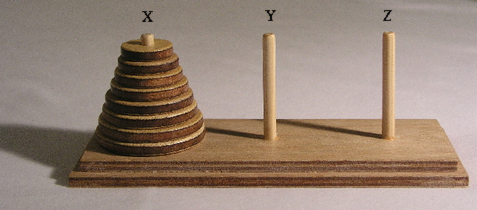
\includegraphics[width=180pt]{Tower-of-Hanoi.png}\\
\figcaption{Hanoi塔问题}\label{fig:hanoiTower}
\end{center}


现要求将X塔上的n个圆盘移动到Z上并仍按同样的顺序叠放,圆盘移动时必须遵循下列规则:
\begindot
\item 每次只能移动一个圆盘;
\item 圆盘可以插在X、Y和Z中的任一塔座上;
\item 任何时刻都不能将一个较大的圆盘压在较小的圆盘之上。
\myenddot
 
给出一个数$n$,求出最少步数的移动序列。


\subsubsection{输入}
一个整数 $n, n \leq 10$


\subsubsection{输出}
第一行一个整数$k$,表示最少的移动步数。

接下来$k$行,每行一句话,N from X to Y,表示把N号盘从X柱移动到Y柱。X,Y 属于\fn{\{'A','B','C'\}}


\subsubsection{样例输入}
\begin{Code}
3
\end{Code}


\subsubsection{样例输出}
\begin{Code}
7
1 from A to C
2 from A to B
1 from C to B
3 from A to C
1 from B to A
2 from B to C
1 from A to C
\end{Code}

\subsubsection{分析}
用递归。


\subsubsection{代码}

\begin{Codex}[label=hanoi.c]
#include <stdio.h>

/*
 * @brief 将塔座x上按直径有小到大且自上而下编号
 * 为1至n的n个圆盘按规则搬到塔座z上,y可用做辅助塔座.
 * @param[in] n 圆盘个数
 * @param[in] x 源塔座
 * @param[in] y 辅助塔座
 * @param[in] z 目标塔座
 * @return 无
 */
void hanoi(int n, char x, char y, char z) {
    if(n ==  1) {
        /* 将编号为n的圆盘从x移到z */
        printf("%d from %c to %c\n", n, x, z);
        return;
    } else {
        /* 将x上编号1至n-1的圆盘移到y,z作辅助塔 */
        hanoi(n-1, x, z, y);
        /* 将编号为n的圆盘从x移到z */
        printf("%d from %c to %c\n", n, x, z);
        /* 将y上编号1至n-1的圆盘移到z,x作辅助塔 */
        hanoi(n-1, y, x, z);
    }
}

int main() {
    int n;
    scanf("%d", &n);
    printf("%d\n", (1 << n) - 1); /* 总次数 */
    hanoi(n, 'A', 'B', 'C');
    return 0;
}
\end{Codex}


\subsubsection{相关的题目}
与本题相同的题目:
\begindot
\item wikioi 3145 汉诺塔游戏 , \myurl{http://www.wikioi.com/problem/3145/}
\myenddot

与本题相似的题目:
\begindot
\item  无
\myenddot


\subsection{进制转换}
\begin{Codex}[label=convert_base.cpp]
#include <stack>
#include <cstdio>

 /**
  * @brief 进制转换,将一个10进制整数转化为 d进制,d<=16.
  * @param[in] n 整数n
  * @param[in] d d进制
  * @return 无
  */
void convert_base(int n, const int d) {
    stack<int> s;
    int e;

    while(n != 0) {
        e = n % d;
        s.push(e);
        n /= d;
    }
    while(!s.empty()) {
        e = s.top();
        s.pop();
        printf("%X", e);
    }
    return;
}

const int MAXN = 64; // 栈的最大长度
int stack[MAXN];
int top = -1;
/**
 * @brief 进制转换,将一个10进制整数转化为 d进制,d<=16,更优化的版本.
 *
 * 如果可以预估栈的最大空间,则用数组来模拟栈,这时常用的一个技巧。
 * 这里,栈的最大长度是多少?假设CPU是64位,最大的整数则是2^64,由于
 * 数制最小为2,在这个进制下,数的位数最长,这就是栈的最大长度,最长为64。
 *
 * @param[in] n 整数n
 * @param[in] d d进制
 * @return 无
 */
void convert_base2(int n, const int d) {
    int e;

    while(n != 0) {
        e = n % d;
        stack[++top] = e; // push
        n /= d;
    }
    while(top >= 0) {
        e = stack[top--]; // pop
        printf("%X", e);
    }
    return;
}


/**
 * @brief 进制转换,将一个d进制整数转化为10进制,d<=16.
 * @param[in] s d进制整数
 * @param[in] d d进制
 * @return 10进制整数
 */
int restore(const char s[MAXN], const int d) {
    int result = 0;
    int one;

    for (int i = 0; s[i] != '\0'; i++) {
        if (s[i] >= '0' && s[i] <= '9') one = s[i] - '0';
        else if (s[i] >= 'A' && s[i] <= 'F') one = s[i] - 'A' + 10;
        else one = s[i] - 'a' + 10; /* (s[i] >= 'a' && s[i] <= 'f') */
        
        result = result * d + one;
    }
    return result;
}
\end{Codex}


\subsection{Design Queue by Stack}
Design a queue (FIFO) structure using only stacks (LIFO). 

Code is not necessary. 

Follow-up: provide a complexity analysis of push and remove operations.

\section{队列} %%%%%%%%%%%%%%%%%%%%%%%%%%%%%%


\subsection{打印杨辉三角}

\begin{Codex}[label=yanghui_triangle.cpp]
#include <queue>
/**
 * @brief 打印杨辉三角系数.
 *
 * 分行打印二项式(a+b)^n展开式的系数。在输出上一行
 * 系数的同时,将其下一行的系数预先计算好,放入队列中。
 * 在各行系数之间插入一个0。
 *
 * @param[in] n (a+b)^n
 * @return 无
 */
void yanghui_triangle(const int n) {
    queue<int> q;
    /* 预先放入第一行的1 */
    q.push(1);

    for(int i = 0; i <= n; i++) {     /* 逐行处理*/
        int s = 0;
        q.push(s);      /* 在各行间插入一个0*/

        /* 处理第i行的i+2个系数(包括一个0)*/
        for(int j = 0; j < i+2; j++) {
            int t;
            int tmp;
            t = q.front();  /*读取一个系数,放入t*/
            q.pop();
            tmp = s + t;      /* 计算下一行系数,并进队列*/
            q.push(tmp);
            s = t;            /* 打印一个系数,第i+2个是0*/
            if(j != i+1) {
                printf("%d ",s);
            }
        }
        printf("\n");
    }
}
\end{Codex}

\chapter{树}

\section{BST} %%%%%%%%%%%%%%%%%%%%%%%%%%%%%%
\label{sec:binarySearchTree}

Given a BST and a number x, check whether exists two nodes in the BST whose sum equals to x. You can not use one extra array to serialize the BST and do a 2sum solver on it.

\subsubsection{相关题目}
\begindot
\item 2Sum, 见 \S \ref{sec:Two-sum}
\item 3Sum, 见 \S \ref{sec:3sum}
\item 3Sum Closest, 见 \S \ref{sec:3sum-closest}
\item 4Sum, 见 \S \ref{sec:4sum}
\myenddot

\section{二叉树的遍历} %%%%%%%%%%%%%%%%%%%%%%%%%%%%%%
\label{sec:binaryTreeTraversal}

在中序遍历中,一个节点的前驱,是其左子树的最右下角结点,后继,是其右子树的最左下角结点。

在后序遍历中,
\begindot
\item 若结点是根结点,则其后继为空;
\item 若结点是双亲的右子树,或是左子树但双亲无右子树,则其后继为双亲结点;
\item 若结点是双亲的左子树且双亲有右子树,则其后继为右子树按后序遍历的第一个结点
\myenddot


\begin{Codex}[label=binary_tree.cpp]
#include <iostream>
#include <stack>
#include <queue>

/** 结点的数据 */
typedef int tree_node_elem_t;
 /*
  *@struct
  *@brief 二叉树结点
  */
struct binary_tree_node_t {
    binary_tree_node_t *left;   /* 左孩子*/
    binary_tree_node_t *right;   /* 右孩子*/
    tree_node_elem_t elem; /* 结点的数据*/
};

/**
  * @brief 先序遍历,递归.
  * @param[in] root 根结点
  * @param[in] visit 访问数据元素的函数指针
  * @return 无
  */
void pre_order_r(const binary_tree_node_t *root,
                 int (*visit)(const binary_tree_node_t*)) {
    if (root == nullptr) return;

    visit(root);
    pre_order_r(root->left, visit);
    pre_order_r(root->right, visit);
}

/**
  * @brief 中序遍历,递归.
  */
void in_order_r(const binary_tree_node_t *root,
                int (*visit)(const binary_tree_node_t*)) {
    if(root == nullptr) return;

    in_order_r(root->left, visit);
    visit(root);
    in_order_r(root->right, visit);
}

/**
  * @brief 后序遍历,递归.
  */
void post_order_r(const binary_tree_node_t *root,
                  int (*visit)(const binary_tree_node_t*)) {
    if(root == nullptr) return;

    post_order_r(root->left, visit);
    post_order_r(root->right, visit);
    visit(root);
}

/**
 * @brief 先序遍历,非递归.
 */
void pre_order(const binary_tree_node_t *root,
               int (*visit)(const binary_tree_node_t*)) {
    const binary_tree_node_t *p;
    stack<const binary_tree_node_t *> s;

    p = root;

    if(p != nullptr) s.push(p);

    while(!s.empty()) {
        p = s.top();
        s.pop();
        visit(p);

        if(p->right != nullptr) s.push(p->right);
        if(p->left != nullptr) s.push(p->left);
    }
}

/**
 * @brief 中序遍历,非递归.
 */
void in_order(const binary_tree_node_t *root,
              int (*visit)(const binary_tree_node_t*)) {
    const binary_tree_node_t *p;
    stack<const binary_tree_node_t *> s;

    p = root;

    while(!s.empty() || p!=nullptr) {
        if(p != nullptr) {
            s.push(p);
            p = p->left;
        } else {
            p = s.top();
            s.pop();
            visit(p);
            p = p->right;
        }
    }
}

/**
 * @brief 后序遍历,非递归.
 */
void post_order(const binary_tree_node_t *root,
                int (*visit)(const binary_tree_node_t*)) {
    /* p,正在访问的结点,q,刚刚访问过的结点*/
    const binary_tree_node_t *p, *q;
    stack<const binary_tree_node_t *> s;

    p = root;

    do {
        while(p != nullptr) { /* 往左下走*/
            s.push(p);
            p = p->left;
        }
        q = nullptr;
        while(!s.empty()) {
            p = s.top();
            s.pop();
            /* 右孩子不存在或已被访问,访问之*/
            if(p->right == q) {
                visit(p);
                q = p; /* 保存刚访问过的结点*/
            } else {
                /* 当前结点不能访问,需第二次进栈*/
                s.push(p);
                /* 先处理右子树*/
                p = p->right;
                break;
            }
        }
    } while(!s.empty());
}

/**
 * @brief 层次遍历,也即BFS.
 *
 * 跟先序遍历一模一样,唯一的不同是栈换成了队列
 */
void level_order(const binary_tree_node_t *root,
                int (*visit)(const binary_tree_node_t*)) {
    const binary_tree_node_t *p;
    queue<const binary_tree_node_t *> q;

    p = root;

    if(p != nullptr) q.push(p);

    while(!q.empty()) {
        p = q.front();
        q.pop();
        visit(p);

        /*先左后右或先右后左无所谓*/
        if(p->left != nullptr) q.push(p->left);
        if(p->right != nullptr) q.push(p->right);
    }
}
\end{Codex}

\section{线索二叉树} %%%%%%%%%%%%%%%%%%%%%%%%%%%%%%
二叉树中存在很多空指针,可以利用这些空指针,指向其前驱或者后继。这种利用起来的空指针称为线索,这种改进后的二叉树称为线索二叉树(threaded binary tree)。

一棵n个结点的二叉树含有n+1个空指针。这是因为,假设叶子节点数为$n_0$,度为1的节点数为$n_1$,度为2的节点数为$n_2$,每个叶子节点有2个空指针,每个度为1的节点有1个空指针,则空指针的总数为$2n_0+n_1$,又有$n_0=n_2+1$(留给读者证明),因此空指针总数为$2n_0+n_1=n_0+n_2+1+n_1=n_0+n_1+n_2+1=n+1$。

在二叉树线索化过程中,通常规定,若无左子树,令left指向前驱,若无右子树,令rchild指向后继。还需要增加两个标志域表示当前指针是不是线索,例如ltag=1,表示left指向的是前驱,ltag=0,表示left指向的是左孩子,rtag类似。

二叉树的线索化,实质上就是遍历一棵树,只是在遍历的过程中,检查当前节点的左右指针是否为空,若为空,将它们改为指向前驱或后继的线索。

以中序线索二叉树为例,指针pre表示前驱,succ表示后继,如图~\ref{fig:threadedBinaryTree}所示。

\begin{center}
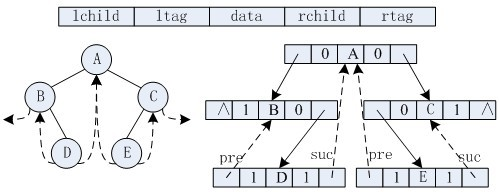
\includegraphics[width=300pt]{threaded-binary-tree.png} \\
\figcaption{中序线索二叉树}\label{fig:threadedBinaryTree}
\end{center}

在中序线索二叉树中,一个节点的前驱,是其左子树的最右下角结点,后继,是其右子树的最左下角结点。

中序线索二叉树的C语言实现如下。
\begin{Codex}[label=theaded_binary_tree.c]
/** @file threaded_binary_tree.c
  * @brief 线索二叉树.
  */
#include <stddef.h>    /* for NULL */
#include <stdio.h>

/* 结点数据的类型. */
typedef int elem_t;

 /**
  *@struct
  *@brief 线索二叉树结点.
  */
typedef struct tbt_node_t {
    int ltag; /** 1表示是线索,0表示是孩子 */
    int rtag; /** 1表示是线索,0表示是孩子 */
    struct tbt_node_t *left; /** 左孩子*/
    struct tbt_node_t *right; /** 右孩子*/
    elem_t elem; /** 结点所存放的数据*/
}tbt_node_t;

/* 内部函数 */
static void in_thread(tbt_node_t *p, tbt_node_t **pre);
static tbt_node_t *first(tbt_node_t *p);
static tbt_node_t *next(const tbt_node_t *p);

 /**
  * @brief 建立中序线索二叉树.
  * @param[in] root 树根
  * @return 无
  */
void create_in_thread(tbt_node_t *root) {
    /* 前驱结点指针*/
    tbt_node_t *pre=NULL;
    if(root != NULL) { /* 非空二叉树,线索化*/
        /* 中序遍历线索化二叉树*/
        in_thread(root, &pre);
        /* 处理中序最后一个结点*/
        pre->right = NULL;
        pre->rtag = 1;
    }
}


/**
  * @brief 在中序线索二叉树上执行中序遍历.
  * @param[in] root 树根
  * @param[in] visit 访问结点的数据的函数
  * @return 无
  */
void in_order(tbt_node_t *root, int(*visit)(tbt_node_t*)) {
    tbt_node_t *p;
    for(p = first(root); p != NULL; p = next(p)) {
        visit(p);
    }
}


 /*
  * @brief 中序线索化二叉树的主过程.
  * @param[in] p 当前要处理的结点
  * @param[inout] pre 当前结点的前驱结点
  * @return 无
  */
static void in_thread(tbt_node_t *p, tbt_node_t **pre) {
    if(p != NULL) {
        in_thread(p->left, pre); /* 线索化左子树 */
        if(p->left == NULL) {  /* 左子树为空,建立前驱 */
            p->left = *pre;
            p->ltag = 1;
        }
        /* 建立前驱结点的后继线索 */
        if((*pre) != NULL &&
            (*pre)->right == NULL) {
            (*pre)->right = p;
            (*pre)->rtag = 1;
        }
        *pre = p; /* 更新前驱 */
        in_thread(p->right, pre); /* 线索化右子树 */
    }
}

 /*
  * @brief 寻找线索二叉树的中序下的第一个结点.
  * @param[in] p 线索二叉树中的任意一个结点
  * @return 此线索二叉树的第一个结点
  */
static tbt_node_t *first(tbt_node_t *p) {
    if(p == NULL)  return NULL;

    while(p->ltag == 0) {
        p = p->left;  /* 最左下结点,不一定是叶结点*/
    }
    return p;
}

 /*
  * @brief 求中序线索二叉树中某结点的后继.
  * @param[in] p 某结点
  * @return p的后继
  */
static tbt_node_t *next(const tbt_node_t *p) {
    if(p->rtag == 0) {
        return first(p->right);
    } else {
        return p->right;
    }
}
\end{Codex}

中序线索二叉树最简单,在中序线索的基础上稍加修改就可以实现先序,后续就要再费点心思了。


\section{Morris Traversal} %%%%%%%%%%%%%%%%%%%%%%%%%%%%%%
通过前面第\S \ref{sec:binaryTreeTraversal}节,我们知道,实现二叉树的前序(preorder)、中序(inorder)、后序(postorder)遍历有两个常用的方法,一是递归(recursive),二是栈(stack+iterative)。这两种方法都是O(n)的空间复杂度。

而Morris Traversal只需要O(1)的空间复杂度。这种算法跟线索二叉树很像,不过Morris Traversal一边建线索,一边访问数据,访问完后销毁线索,保持二叉树不变。

\subsection{Morris中序遍历}
Morris中序遍历的步骤如下:
\begin{enumerate}
\item 初始化当前节点cur为root节点
\item 如果cur没有左孩子,则输出当前节点并将其右孩子作为当前节点,即cur = cur->rchild。
\item 如果cur有左孩子,则寻找cur的前驱,即cur的左子树的最右下角结点。\\
   a) 如果前驱节点的右孩子为空,将它的右孩子指向当前节点,当前节点更新为当前节点的左孩子。\\
   b) 如果前驱节点的右孩子为当前节点,将它的右孩子重新设为空(恢复树的形状),输出当前节点,当前节点更新为当前节点的右孩子。
\item 重复2、3步骤,直到cur为空。
\end{enumerate}
如图~\ref{fig:inorderMorris}所示,cur表示当前节点,深色节点表示该节点已输出。

\begin{center}
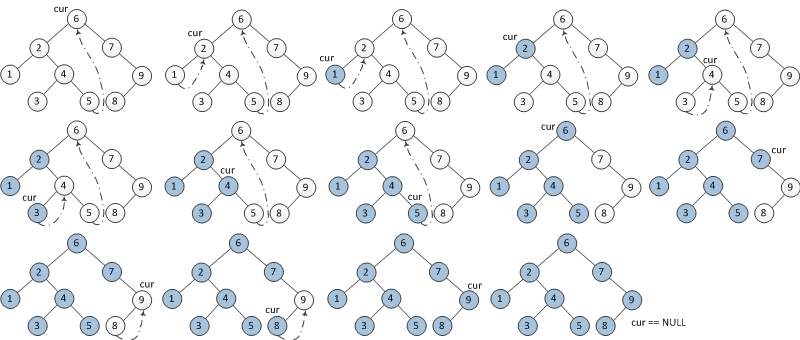
\includegraphics[width=360pt]{inorder-morris-traversal.png} \\
\figcaption{Morris中序遍历}\label{fig:inorderMorris}
\end{center}

C语言实现见第\S\ref{sec:morrisTraversalImpl}节。

\subsubsection{相关的题目}
\begindot
\item Leet Code - Binary Tree Inorder Traversal, \myurl{http://leetcode.com/onlinejudge\#question_94}
\myenddot


\subsection{Morris先序遍历}
Morris先序遍历的步骤如下:
\begin{enumerate}
\item 初始化当前节点cur为root节点
\item 如果cur没有左孩子,则输出当前节点并将其右孩子作为当前节点,即cur = cur->rchild。
\item 如果cur有左孩子,则寻找cur的前驱,即cur的左子树的最右下角结点。\\
   a) 如果前驱节点的右孩子为空,将它的右孩子指向当前节点,\textbf{输出当前节点(在这里输出,这是与中序遍历唯一的不同点)}当前节点更新为当前节点的左孩子。\\
   b) 如果前驱节点的右孩子为当前节点,将它的右孩子重新设为空(恢复树的形状),\sout{输出当前节点,}当前节点更新为当前节点的右孩子。
\item 重复2、3步骤,直到cur为空。
\end{enumerate}
如图~\ref{fig:preorderMorris}所示。

\begin{center}
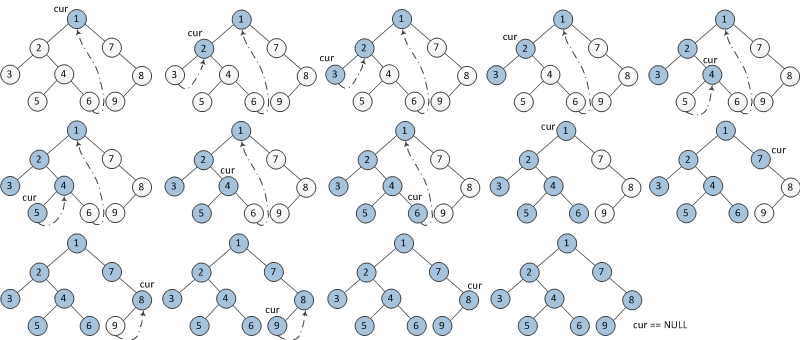
\includegraphics[width=360pt]{preorder-morris-traversal.png} \\
\figcaption{Morris先序遍历}\label{fig:preorderMorris}
\end{center}

C语言实现见第\S\ref{sec:morrisTraversalImpl}节。


\subsection{Morris后序遍历}
Morris后续遍历稍微复杂,需要建立一个临时节点dump,令其左孩子是root,并且还需要一个子过程,就是倒序输出某两个节点之间路径上的所有节点。

Morris后序遍历的步骤如下:
\begin{enumerate}
\item 初始化当前节点cur为root节点
\item 如果cur没有左孩子,则\sout{输出当前节点并}将其右孩子作为当前节点,即cur = cur->rchild。
\item 如果cur有左孩子,则寻找cur的前驱,即cur的左子树的最右下角结点。\\
   a) 如果前驱节点的右孩子为空,将它的右孩子指向当前节点,当前节点更新为当前节点的左孩子。\\
   b) 如果前驱节点的右孩子为当前节点,将它的右孩子重新设为空(恢复树的形状),\sout{输出当前节点,}\textbf{倒序输出从当前节点的左孩子到该前驱节点这条路径上的所有节点。}当前节点更新为当前节点的右孩子。
\item 重复2、3步骤,直到cur为空。
\end{enumerate}
如图~\ref{fig:postorderMorris}所示。

\begin{center}
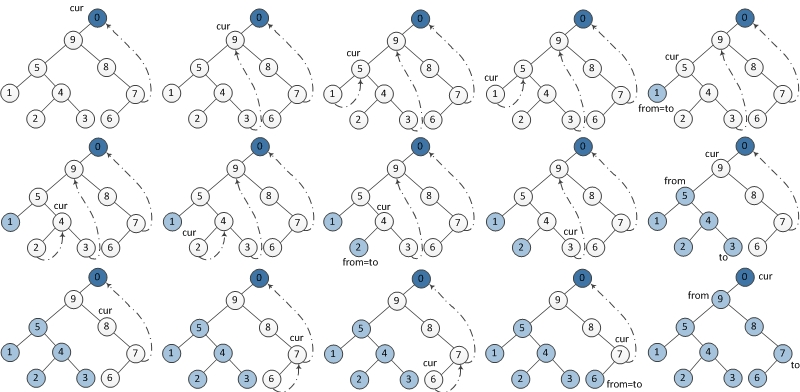
\includegraphics[width=360pt]{postorder-morris-traversal.png} \\
\figcaption{Morris后序遍历}\label{fig:postorderMorris}
\end{center}

C语言实现见第\S\ref{sec:morrisTraversalImpl}节。


\subsection{C语言实现}
\label{sec:morrisTraversalImpl}
\begin{Codex}[label=morris_traversal.c]
/** @file morris_traversal.c
 * @brief Morris遍历算法.
 */
#include<stdio.h>
#include<stdlib.h>

/* 结点数据的类型. */
typedef int elem_t;

/**
 *@struct
 *@brief 二叉树结点.
 */
typedef struct bt_node_t {
    elem_t elem; /* 节点的数据 */
    struct bt_node_t *left; /* 左孩子 */
    struct bt_node_t *right; /* 右孩子 */
} bt_node_t;

/**
 * @brief 中序遍历,Morris算法.
 * @param[in] root 根节点
 * @param[in] visit 访问函数
 * @return 无
 */
void in_order_morris(bt_node_t *root, int(*visit)(bt_node_t*)) {
    bt_node_t *cur, *prev;

    cur = root;
    while (cur != NULL ) {
        if (cur->left == NULL ) {
            visit(cur);
            prev = cur;
            cur = cur->right;
        } else {
            /* 查找前驱 */
            bt_node_t *node = cur->left;
            while (node->right != NULL && node->right != cur)
                node = node->right;

            if (node->right == NULL ) { /* 还没线索化,则建立线索 */
                node->right = cur;
                /* prev = cur; 不能有这句,cur还没有被访问 */
                cur = cur->left;
            } else {    /* 已经线索化,则访问节点,并删除线索  */
                visit(cur);
                node->right = NULL;
                prev = cur;
                cur = cur->right;
            }
        }
    }
}

/**
 * @brief 先序遍历,Morris算法.
 * @param[in] root 根节点
 * @param[in] visit 访问函数
 * @return 无
 */
void pre_order_morris(bt_node_t *root, int (*visit)(bt_node_t*)) {
    bt_node_t *cur, *prev;

    cur = root;
    while (cur != NULL ) {
        if (cur->left == NULL ) {
            visit(cur);
            prev = cur; /* cur刚刚被访问过 */
            cur = cur->right;
        } else {
            /* 查找前驱 */
            bt_node_t *node = cur->left;
            while (node->right != NULL && node->right != cur)
                node = node->right;

            if (node->right == NULL ) { /* 还没线索化,则建立线索 */
                visit(cur); /* 仅这一行的位置与中序不同 */
                node->right = cur;
                prev = cur; /* cur刚刚被访问过 */
                cur = cur->left;
            } else {    /* 已经线索化,则删除线索  */
                node->right = NULL;
                /* prev = cur; 不能有这句,cur已经被访问 */
                cur = cur->right;
            }
        }
    }
}


static void reverse(bt_node_t *from, bt_node_t *to);
static void visit_reverse(bt_node_t* from, bt_node_t *to,
        int (*visit)(bt_node_t*));
/**
 * @brief 后序遍历,Morris算法.
 * @param[in] root 根节点
 * @param[in] visit 访问函数
 * @return 无
 */
void post_order_morris(bt_node_t *root, int (*visit)(bt_node_t*)) {
    bt_node_t dummy = { 0, NULL, NULL };
    bt_node_t *cur, *prev = NULL;

    dummy.left = root;
    cur = &dummy;
    while (cur != NULL ) {
        if (cur->left == NULL ) {
            prev = cur; /* 必须要有 */
            cur = cur->right;
        } else {
            bt_node_t *node = cur->left;
            while (node->right != NULL && node->right != cur)
                node = node->right;

            if (node->right == NULL ) { /* 还没线索化,则建立线索 */
                node->right = cur;
                prev = cur; /* 必须要有 */
                cur = cur->left;
            } else { /* 已经线索化,则访问节点,并删除线索  */
                visit_reverse(cur->left, prev, visit);  // call print
                prev->right = NULL;
                prev = cur; /* 必须要有 */
                cur = cur->right;
            }
        }
    }
}

/*
 * @brief 逆转路径.
 * @param[in] from from
 * @param[to] to to
 * @return 无
 */
static void reverse(bt_node_t *from, bt_node_t *to) {
    bt_node_t *x = from, *y = from->right, *z;
    if (from == to) return;

    while (x != to) {
        z = y->right;
        y->right = x;
        x = y;
        y = z;
    }
}

/*
 * @brief  访问逆转后的路径上的所有结点.
 * @param[in] from from
 * @param[to] to to
 * @return 无
 */
static void visit_reverse(bt_node_t* from, bt_node_t *to,
        int (*visit)(bt_node_t*)) {
    bt_node_t *p = to;
    reverse(from, to);

    while (1) {
        visit(p);
        if (p == from)
            break;
        p = p->right;
    }

    reverse(to, from);
}

/*
 * @brief 分配一个新节点.
 * @param[in] e 新节点的数据
 * @return 新节点
 */
bt_node_t* new_node(int e) {
    bt_node_t* node = (bt_node_t*) malloc(sizeof(bt_node_t));
    node->elem = e;
    node->left = NULL;
    node->right = NULL;

    return (node);
}

static int print(bt_node_t *node) {
    printf(" %d ", node->elem);
    return 0;
}

/* test */
int main() {
    /* 构造的二叉树如下
       1
     /   \
    2      3
  /  \
4     5
     */
    bt_node_t *root = new_node(1);
    root->left = new_node(2);
    root->right = new_node(3);
    root->left->left = new_node(4);
    root->left->right = new_node(5);

    in_order_morris(root, print);
    printf("\n");
    pre_order_morris(root, print);
    printf("\n");
    post_order_morris(root, print);
    printf("\n");

    return 0;
}
\end{Codex}


\section{重建二叉树} %%%%%%%%%%%%%%%%%%%%%%%%%%%%%%
\begin{Codex}[label=binary_tree_rebuild.c]
#include <stdio.h>
#include <stdlib.h>
#include <string.h>
#include <stddef.h>
/**
 * @brief 给定前序遍历和中序遍历,输出后序遍历.
 *
 * @param[in] pre 前序遍历的序列
 * @param[in] in 中序遍历的序列
 * @param[in] n 序列的长度
 * @param[out] post 后续遍历的序列
 * @return 无
 */
void build_post(const char * pre, const char *in, const int n, char *post) {
    int left_len = strchr(in, pre[0]) - in;
    if(n <= 0) return;
    
    build_post(pre + 1, in, left_len, post);
    build_post(pre + left_len + 1, in + left_len + 1,
            n - left_len - 1, post + left_len);
    post[n - 1] = pre[0];
}

#define MAX  64
// 测试
// BCAD CBAD,输出 CDAB
// DBACEGF ABCDEFG,输出 ACBFGED
void build_post_test() {
    char pre[MAX] = {0};
    char in[MAX] = {0};
    char post[MAX] = {0};
    int n;

    scanf("%s%s", pre, in);
    n = strlen(pre);

    build_post(pre, in, n, post);
    printf("%s\n", post);
}

/* 结点数据的类型. */
typedef char elem_t;

/**
 *@struct
 *@brief 二叉树结点.
 */
typedef struct bt_node_t {
    elem_t elem; /* 节点的数据 */
    struct bt_node_t *left; /* 左孩子 */
    struct bt_node_t *right; /* 右孩子 */
} bt_node_t;

/**
 * @brief 给定前序遍历和中序遍历,重建二叉树.
 *
 * @param[in] pre 前序遍历的序列
 * @param[in] in 中序遍历的序列
 * @param[in] n 序列的长度
 * @param[out] root 根节点
 * @return 无
 */
void rebuild(const char *pre, const char *in, int n, bt_node_t **root) {
    int left_len;
    // 检查终止条件
    if (n <= 0 || pre == NULL || in == NULL)
        return;
    //获得前序遍历的第一个结点
    *root = (bt_node_t*) malloc(sizeof(bt_node_t));
    (*root)->elem = *pre;
    (*root)->left = NULL;
    (*root)->right = NULL;

    left_len = strchr(in, pre[0]) - in;
    //重建左子树
    rebuild(pre + 1, in, left_len, &((*root)->left));
    //重建右子树
    rebuild(pre + left_len + 1, in + left_len + 1, n - left_len - 1,
            &((*root)->right));
}

void print_post_order(const bt_node_t *root) {
    if(root != NULL) {
        print_post_order(root->left);
        print_post_order(root->right);
        printf("%c", root->elem);
    }
}

void rebuild_test() {
    char pre[MAX] = { 0 };
    char in[MAX] = { 0 };
    int n;
    bt_node_t *root;
    scanf("%s%s", pre, in);
    n = strlen(pre);
    
    rebuild(pre, in, n, &root);
    print_post_order(root);
}

int main() {
    build_post_test();
    rebuild_test();
    return 0;
}
\end{Codex}


\section{堆} %%%%%%%%%%%%%%%%%%%%%%%%%%%%%%

\subsection{原理和实现}
C++可以直接使用\fn{priority_queue}。

\begin{Codex}[label=heap.c]
/** @file heap.c
 * @brief 堆,默认为小根堆,即堆顶为最小.
 * @author soulmachine@gmail.com
 */
#include <stdlib.h>  /* for malloc() */
#include <string.h>  /* for memcpy() */

typedef int heap_elem_t; // 元素的类型

/**
 * @struct
 * @brief 堆的结构体
 */
typedef struct heap_t {
    int     size;   /** 实际元素个数 */
    int     capacity; /** 容量,以元素为单位 */
    heap_elem_t  *elems;   /** 堆的数组 */
    int (*cmp)(const heap_elem_t*, const heap_elem_t*);   /** 元素的比较函数 */
}heap_t;


/** 基本类型(如int, long, float, double)的比较函数 */
int cmp_int(const int *x, const int *y) {
    const int sub = *x - *y;
    if(sub > 0) {
        return 1;
    } else if(sub < 0) {
        return -1;
    } else {
        return 0;
    }
}

/**
 * @brief 创建堆.
 * @param[out] capacity 初始容量
 * @param[in] cmp cmp 比较函数,小于返回-1,等于返回0
 *            大于返回1,反过来则是大根堆
 * @return 成功返回堆对象的指针,失败返回 NULL
 */
heap_t* heap_create(const int capacity,
        int (*cmp)(const heap_elem_t*, const heap_elem_t*)) {
    heap_t *h = (heap_t*)malloc(sizeof(heap_t));
    h->size = 0;
    h->capacity = capacity;
    h->elems = (heap_elem_t*)malloc(capacity * sizeof(heap_elem_t));
    h->cmp = cmp;

    return h;
}

/**
 * @brief 销毁堆.
 * @param[inout] h 堆对象的指针
 * @return 无
 */
void heap_destroy(heap_t *h) {
    free(h->elems);
    free(h);
}


/**
 * @brief 判断堆是否为空.
 * @param[in] h 堆对象的指针
 * @return 是空,返回 1,否则返回 0
 */
int heap_empty(const heap_t *h) {
    return h->size == 0;
}

/**
 * @brief 获取元素个数.
 * @param[in] s 堆对象的指针
 * @return 元素个数
 */
int heap_size(const heap_t *h) {
    return h->size;
}

/*
 * @brief 小根堆的自上向下筛选算法.
 * @param[in] h 堆对象的指针
 * @param[in] start 开始结点
 * @return 无
 */
void heap_sift_down(const heap_t *h, const int start) {
    int i = start;
    int j;
    const heap_elem_t tmp = h->elems[start];

    for(j = 2 * i + 1; j < h->size; j = 2 * j + 1) {
        if(j < (h->size - 1) &&
            // h->elems[j] > h->elems[j + 1]
            h->cmp(&(h->elems[j]), &(h->elems[j + 1])) > 0) {
                j++; /* j 指向两子女中小者*/
        }
        // tmp <= h->data[j]
        if(h->cmp(&tmp, &(h->elems[j])) <= 0) {
            break;
        } else {
            h->elems[i] = h->elems[j];
            i = j;
        }
    }
    h->elems[i] = tmp;
}

/*
 * @brief 小根堆的自下向上筛选算法.
 * @param[in] h 堆对象的指针
 * @param[in] start 开始结点
 * @return 无
 */
void heap_sift_up(const heap_t *h, const int start) {
    int j = start;
    int i= (j - 1) / 2;
    const heap_elem_t tmp = h->elems[start];

    while(j > 0) {
        // h->data[i] <= tmp
        if(h->cmp(&(h->elems[i]), &tmp) <= 0) {
            break;
        } else {
            h->elems[j] = h->elems[i];
            j = i;
            i = (i - 1) / 2;
        }
    }
    h->elems[j] = tmp;
}

/**
 * @brief 添加一个元素.
 * @param[in] h 堆对象的指针
 * @param[in] x 要添加的元素
 * @return 无
 */
void heap_push(heap_t *h, const heap_elem_t x) {
    if(h->size == h->capacity) { /*已满,重新分配内存*/
        heap_elem_t* tmp =
            (heap_elem_t*)realloc(h->elems, h->capacity * 2 * sizeof(heap_elem_t));
        h->elems = tmp;
        h->capacity *= 2;
    }

    h->elems[h->size] = x;
    h->size++;

    heap_sift_up(h, h->size - 1);
}

/**
 * @brief 弹出堆顶元素.
 * @param[in] h 堆对象的指针
 * @return 无
 */
void heap_pop(heap_t *h) {
    h->elems[0] = h->elems[h->size - 1];
    h->size --;
    heap_sift_down(h, 0);
}

/**
 * @brief 获取堆顶元素.
 * @param[in] h 堆对象的指针
 * @return 堆顶元素
 */
heap_elem_t heap_top(const heap_t *h) {
    return h->elems[0];
}
\end{Codex}


\subsection{最小的N个和} %%%%%%%%%%%%%%%%%%%%%%%%%%%%%%
\subsubsection{描述}
有两个长度为$N$的序列 A 和 B,在 A 和 B 中各任取一个数可以得到 $N^2$ 个和,求这$N^2$ 个和中最小的$N$个。

\subsubsection{输入}
第一行输入一个正整数$N$;第二行N个整数$A_i$ 且$A_i \leq 10^9$;第三行$N$个整数$B_i$,且$Bi \leq 10^9$。

\subsubsection{输出}
输出仅一行,包含$N$个整数,从小到大输出这$N$个最小的和,相邻数字之间用空格隔开。

\subsubsection{样例输入}
\begin{Code}
5
1 3 2 4 5 
6 3 4 1 7
\end{Code}

\subsubsection{样例输出}
\begin{Code}
2 3 4 4 5
\end{Code}

\subsubsection{分析}
由于数据太大,有$N^2$个和,不能通过先求和再排序的方式来求解,这个时候就要用到堆了。

首先将A,B两数组排序,我们可以建立这样一个有序表:
\begin{eqnarray}
A_1+B_1<A_1+B_2<A_1+B_3< &...& <A_1+B_N \nonumber \\
A_2+B_1<A_2+B_2<A_2+B_3< &...& <A_2+B_N \nonumber \\
& ...  \nonumber \\
A_N+B_1<A_N+B_2<A_N+B_3< &...& <A_N+B_N \nonumber
\end{eqnarray}

首先将\fn{A[i] + B[0]}压入堆中,设每次出堆的元素为\fn{sum=A[a]+B[b]},则将\fn{A[a]+B[b+1]}入堆,这样可以保证前$N$个出堆的元素为最小的前$N$项。在实现的时候,可以不用保存B数组的下标,通过\fn{sum-B[b]+B[b+1]}来替换\fn{A[a]+B[b+1]}来节省空间。

\subsubsection{代码}
\begin{Codex}[label=sequence.cpp]
/* wikioi 1245 最小的N个和,http://www.wikioi.com/problem/1245/  */
#include <cstdio>
#include <queue>
#include <algorithm>

const int MAXN = 100000;

int N;
int a[MAXN], b[MAXN];

typedef struct node_t {
    int sum;
    int b; /* sum=a[i]+b[b] */
    bool operator>(const node_t &other) const {
        return sum > other.sum;
    }
} node_t;


void k_merge() {
    sort(a, a+N);
    sort(b, b+N);
    priority_queue<node_t, vector<node_t>,
                                greater<node_t> > q;

    for (int i = 0; i < N; i++) {
        node_t tmp;
        tmp.sum = a[i]+b[0];
        tmp.b = 0;
        q.push(tmp);
    }

    for (int i = 0; i < N; i++) {
        node_t tmp = q.top(); q.pop();
        printf("%d ", tmp.sum);
        tmp.sum = tmp.sum - b[tmp.b] + b[tmp.b + 1];
        tmp.b++;
        q.push(tmp);
    }

    return;
}

int main() {
    scanf("%d", &N);
    for (int i = 0; i < N; i++) {
        scanf("%d", &a[i]);
    }
    for (int i = 0; i < N; i++) {
        scanf("%d", &b[i]);
    }

    k_merge();
    return 0;
}
\end{Codex}

\subsubsection{相关的题目}
与本题相同的题目:
\begindot
\item wikioi 1245 最小的N个和, \myurl{http://www.wikioi.com/problem/1245/}
\myenddot

与本题相似的题目:
\begindot
\item  POJ 2442 Sequence, \myurl{http://poj.org/problem?id=2442}
\myenddot


\section{并查集} %%%%%%%%%%%%%%%%%%%%%%%%%%%%%%

\subsection{原理和实现}
通常用树双亲表示作为并查集的存储结构。每个集合以一棵树表示,数组元素的下标代表元素名,根结点的双亲指针为一个负数,表示集合的元素的个数。如图~\ref{fig:ufs1}、图~\ref{fig:ufs2}和图~\ref{fig:ufs3}所示。

\begin{center}
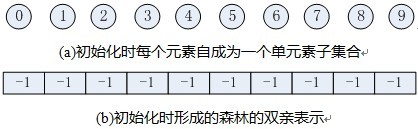
\includegraphics[width=280pt]{ufs1.png}\\
\figcaption{并查集的初始化}\label{fig:ufs1}
\end{center}

\begin{center}
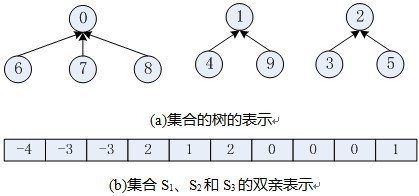
\includegraphics[width=280pt]{ufs2.png}\\
\figcaption{用树表示并查集}\label{fig:ufs2}
\end{center}

\begin{center}
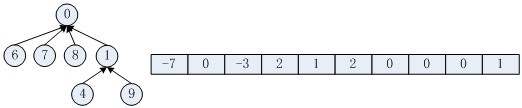
\includegraphics[width=380pt]{ufs3.png}\\
\figcaption{两个集合的并}\label{fig:ufs3}
\end{center}

并查集的C语言实现如下。

\begin{Codex}[label=ufs.c]
#include <stdlib.h>

/** 并查集. */
typedef struct ufs_t {
    int *p;     /** 树的双亲表示法 */
    int size;   /** 大小. */
} ufs_t;

/**
 * @brief 创建并查集.
 * @param[in] n 数组的容量
 * @return 并查集
 */
ufs_t* ufs_create(int n) {
    ufs_t *ufs = (ufs_t*)malloc(sizeof(ufs_t));
    int i;
    ufs->p = (int*)malloc(n * sizeof(int));
    for(i = 0; i < n; i++)
        ufs->p[i] = -1;
    return ufs;
}

/**
 * @brief 销毁并查集.
 * @param[in] ufs 并查集
 * @return 无
 */
void ufs_destroy(ufs_t *ufs) {
    free(ufs->p);
    free(ufs);
}

/**
 * @brief Find操作,带路径压缩,递归版.
 * @param[in] s 并查集
 * @param[in] x 要查找的元素
 * @return 包含元素x的树的根
 */
int ufs_find(ufs_t *ufs, int x) {
    if (ufs->p[x] < 0) return x; // 终止条件

    return ufs->p[x] = ufs_find(ufs, ufs->p[x]); /* 回溯时的压缩路径 */
}

/** Find操作,朴素版, deprecated. */
static int ufs_find_naive(ufs_t *ufs, int x) {
    while (ufs->p[x] >= 0) {
        x = ufs->p[x];
    }
    return x;
}

/** Find操作,带路径压缩,迭代版. */
static int ufs_find_iterative(ufs_t *ufs, int x) {
    int oldx = x; /* 记录原始x */
    while (ufs->p[x] >= 0) {
        x = ufs->p[x];
    }
    while (oldx != x) {
        int temp = ufs->p[oldx];
        ufs->p[oldx] = x;
        oldx = temp;
    }
    return x;
}

/**
 * @brief Union操作,将y并入到x所在的集合.
 * @param[in] s 并查集
 * @param[in] x 一个元素
 * @param[in] y 另一个元素
 * @return 如果二者已经在同一集合,并失败,返回-1,否则返回0
 */
int ufs_union(ufs_t *ufs, int x, int y) {
    const int rx = ufs_find(ufs, x);
    const int ry = ufs_find(ufs, y);
    if(rx == ry) return -1;

    ufs->p[rx] += ufs->p[ry];
    ufs->p[ry] = rx;
    return 0;
}

/**
 * @brief 获取元素所在的集合的大小
 * @param[in] ufs 并查集
 * @param[in] x 元素
 * @return 元素所在的集合的大小
 */
int ufs_set_size(ufs_t *ufs, int x) {
    const int rx = ufs_find(ufs, x);
    return -ufs->p[rx];
}
\end{Codex}


\subsection{病毒感染者} %%%%%%%%%%%%%%%%%%%%%%%%%%%%%%
\subsubsection{描述}
一个学校有$n$个社团,一个学生能同时加入不同的社团。由于社团内的同学们交往频繁,如果一个学生感染了病毒,该社团的所有学生都会感染病毒。现在0号学生感染了病毒,问一共有多少个人感染了病毒。

\subsubsection{输入}
输入包含多组测试用例。每个测试用例,第一行包含两个整数$n$,$m$,$n$表示学生个数,$m$表示社团个数。假设$0 < n \leq 30000, 0 \leq m \leq 500$。每个学生从0到$n-1$编号。接下来是$m$行,每行开头是一个整数k,表示该社团的学生个数,接着是$k$个整数表示该社团的学生编号。最后一个测试用例,$n=0,m=0$,表示输入结束。

\subsubsection{输出}
对每个测试用例,输出感染了病毒的学生数目。

\subsubsection{样例输入}
\begin{Code}
100 4
2 1 2
5 10 13 11 12 14
2 0 1
2 99 2
200 2
1 5
5 1 2 3 4 5
1 0
0 0
\end{Code}

\subsubsection{样例输出}
\begin{Code}
4
1
1
\end{Code}

\subsubsection{分析}
非常简单的并查集题目。

\subsubsection{代码}
\begin{Codex}[label=suspects.c]
/* POJ 1611 The Suspects, http://poj.org/problem?id=1611 */
#include <stdio.h>

#define MAXN 30000

/* 等价于复制粘贴,这里为了节约篇幅,使用include,在OJ上提交时请用复制粘贴 */
#include "ufs.c"  /* 见“树->并查集”这节 */

int main() {
    int n, m, k;
    while (scanf("%d%d", &n, &m) && n > 0) {
        ufs_t *ufs = ufs_create(MAXN);
        while (m--) {
            int x, y; /* 两个学生 */
            int rx, ry; /* x, y 所属的集合的根 */
            scanf("%d", &k);

            k--;
            scanf("%d", &x);
            rx = ufs_find(ufs, x);
            while (k--) {
                scanf("%d", &y);
                ry = ufs_find(ufs, y);
                ufs_union(ufs, rx, ry);  /* 只要是跟x同一个集合的都并进去 */
            }
        }
        /* 最后搜索0属于哪个集合,这个集合有多少人 */
        printf("%d\n", ufs_set_size(ufs, 0));
        ufs_destroy(ufs);
    }
    return 0;
}
\end{Codex}

\subsubsection{相关的题目}
与本题相同的题目:
\begindot
\item POJ 1611 The Suspects, \myurl{http://poj.org/problem?id=1611}
\myenddot

与本题相似的题目:
\begindot
\item  None
\myenddot


\subsection{两个黑帮} %%%%%%%%%%%%%%%%%%%%%%%%%%%%%%
\subsubsection{描述}
Tadu城市有两个黑帮帮派,已知有$N$黑帮分子,从1到$N$编号,每个人至少属于一个帮派。每个帮派至少有一个人。给你$M$条信息,有两类信息:
\begindot
\item D a b,明确告诉你,a和b属于不同的帮派 
\item A a b,问你,a和b是否属于不同的帮派
\myenddot

\subsubsection{输入}
第一行是一个整数$T$,表示有$T$组测试用例。每组测试用例的第一行是两个整数$N$和$M$,接下来是$M$行,每行包含一条消息。

\subsubsection{输出}
对每条消息"A a b",基于当前获得的信息,输出判断。答案是"In the same gang.", "In different gangs." 和 "Not sure yet."中的一个。

\subsubsection{样例输入}
\begin{Code}
1
5 5
A 1 2
D 1 2
A 1 2
D 2 4
A 1 4
\end{Code}

\subsubsection{样例输出}
\begin{Code}
Not sure yet.
In different gangs.
In the same gang.
\end{Code}

\subsubsection{分析}
把不在一个集合的节点直接用并查集合并在一起。这样的话,如果询问的2个节点在同一个并查集里面,那么它们之间的关系是确定的,否则无法确定它们的关系。

现在还有一个问题是,在同一个集合里面的2个节点是敌对关系还是朋友关系?可以给每个节点另外附加个信息,记录其距离集合根节点的距离。如果,询问的2个节点距离其根节点的距离都是奇数或者都是偶数,那么这2个节点是朋友关系,否则是敌对关系。

\subsubsection{代码}
\begin{Codex}[label=two_gangs.c]
/* POJ 1703 Find them, Catch them, http://poj.org/problem?id=1703 */
#include <stdio.h>
#include <stdlib.h>

#define MAXN 1000001

/** 并查集. */
typedef struct ufs_t {
    int *p;     /** 树的双亲表示法 */
    int *dist;  /** 到根节点的距离的奇偶性 */
    int size;   /** 大小. */
} ufs_t;

/**
 * @brief 创建并查集.
 * @param[in] ufs 并查集
 * @param[in] ufs 并查集
 * @param[in] n 数组的容量
 * @return 并查集
 */
ufs_t* ufs_create(int n) {
    int i;
    ufs_t *ufs = (ufs_t*)malloc(sizeof(ufs_t));
    ufs->p = (int*)malloc(n * sizeof(int));
    ufs->dist = (int*)malloc(n * sizeof(int));
    for(i = 0; i < n; i++) {
        ufs->p[i] = -1;
        ufs->dist[i] = 0;
    }
    return ufs;
}

/**
 * @brief 销毁并查集.
 * @param[in] ufs 并查集
 * @return 无
 */
void ufs_destroy(ufs_t *ufs) {
    free(ufs->p);
    free(ufs->dist);
    free(ufs);
}

/**
 * @brief Find操作,带路径压缩,递归版.
 * @param[in] s 并查集
 * @param[in] x 要查找的元素
 * @return 包含元素x的树的根
 */
int ufs_find(ufs_t *ufs, int x) {
    if (ufs->p[x] < 0) return x; // 终止条件

    const int parent = ufs->p[x];
    ufs->p[x] = ufs_find(ufs, ufs->p[x]); /* 回溯时的压缩路径 */
    ufs->dist[x] = (ufs->dist[x] + ufs->dist[parent]) % 2;
    return ufs->p[x];
}

/**
 * @brief Union操作,将root2并入到root1.
 * @param[in] s 并查集
 * @param[in] root1 一棵树的根
 * @param[in] root2 另一棵树的根
 * @return 如果二者已经在同一集合,并失败,返回-1,否则返回0
 */
int ufs_union(ufs_t *ufs, int root1, int root2) {
    if(root1 == root2) return -1;
    ufs->p[root1] += ufs->p[root2];
    ufs->p[root2] = root1;
    return 0;
}

/**
 * @brief 添加一对敌人.
 * @param[inout] s 并查集
 * @param[in] x 一对敌人的一个
 * @param[in] y 一对敌人的另一个
 * @return 无
 */
void ufs_add_opponent(ufs_t *ufs, int x, int y) {
    const int rx = ufs_find(ufs, x);
    const int ry = ufs_find(ufs, y);
    ufs_union(ufs, rx, ry);
    /* ry与y关系 + y与x的关系 + x与rx的关系 = ry与rx的关系 */
    ufs->dist[ry] = (ufs->dist[y] + 1 + ufs->dist[x]) % 2;
}

int main() {
    int T;

    scanf("%d", &T);
    while (T--) {
        ufs_t *ufs = ufs_create(MAXN);
        int n, m;
        char c;
        int x, y, rx, ry;
        scanf("%d%d%*c", &n, &m);

        while (m--) {
            scanf("%c%d%d%*c", &c, &x, &y); //注意输入
            rx = ufs_find(ufs, x);
            ry = ufs_find(ufs, y);

            if (c == 'A') {
                if (rx == ry) { //如果根节点相同,则表示能判断关系
                    if (ufs->dist[x] != ufs->dist[y])
                        printf("In different gangs.\n");
                    else
                        printf("In the same gang.\n");
                } else
                    printf("Not sure yet.\n");
            } else if (c == 'D') {
                ufs_add_opponent(ufs, x, y);
            }
        }
        ufs_destroy(ufs);
    }
    return 0;
}
\end{Codex}

\subsubsection{相关的题目}
与本题相同的题目:
\begindot
\item POJ 1703 Find them, Catch them, \myurl{http://poj.org/problem?id=1703}
\myenddot

与本题相似的题目:
\begindot
\item  None
\myenddot


\subsection{食物链} %%%%%%%%%%%%%%%%%%%%%%%%%%%%%%
\subsubsection{描述}
动物王国中有三类动物A,B,C,这三类动物的食物链构成了有趣的环形。A吃B, B吃C,C吃A。 现有$N$个动物,从1到$N$编号。每个动物都是A,B,C中的一种,但是我们并不知道它到底是哪一种。 

有人用两种说法对这N个动物所构成的食物链关系进行描述:
\begindot
\item 第一种说法是"1 X Y",表示X和Y是同类。 
\item 第二种说法是"2 X Y",表示X吃Y。 
\myenddot

此人对$N$个动物,用上述两种说法,一句接一句地说出$K$句话,这$K$句话有的是真的,有的是假的。当一句话满足下列三条之一时,这句话就是假话,否则就是真话。 
\begindot
\item 当前的话与前面的某些真的话冲突,就是假话; 
\item 当前的话中X或Y比N大,就是假话; 
\item 当前的话表示X吃X,就是假话。 
\myenddot

你的任务是根据给定的$N(1 \leq N \leq 50,000)$和$K$句话($0 \leq K \leq 100,000$),输出假话的总数。 

\subsubsection{输入}
第一行是两个整数$N$和$K$,以一个空格分隔。 

以下$K$行每行是三个正整数D,X,Y,两数之间用一个空格隔开,其中D表示说法的种类。
\begindot
\item 若D=1,则表示X和Y是同类。 
\item 若D=2,则表示X吃Y。
\myenddot

\subsubsection{输出}
只有一个整数,表示假话的数目。

\subsubsection{样例输入}
\begin{Code}
100 7
1 101 1 
2 1 2
2 2 3 
2 3 3 
1 1 3 
2 3 1 
1 5 5
\end{Code}

\subsubsection{样例输出}
\begin{Code}
3
\end{Code}

\subsubsection{分析}


\subsubsection{代码}
\begin{Codex}[label=food_chain.c]
/* POJ 1182 食物链, Catch them, http://poj.org/problem?id=1182 */
#include <stdio.h>
#include <stdlib.h>

/** 并查集. */
typedef struct ufs_t {
    int *p;     /** 树的双亲表示法 */
    int *dist;  /** 表示x与父节点p[x]的关系,0表示x与p[x]是同类,
                    1表示x吃p[x],2表示p[x]吃x */
    int size;   /** 大小. */
} ufs_t;

/**
 * @brief 创建并查集.
 * @param[in] ufs 并查集
 * @param[in] n 数组的容量
 * @return 并查集
 */
ufs_t* ufs_create(int n) {
    int i;
    ufs_t *ufs = (ufs_t*)malloc(sizeof(ufs_t));
    ufs->p = (int*)malloc(n * sizeof(int));
    ufs->dist = (int*)malloc(n * sizeof(int));
    for(i = 0; i < n; i++) {
        ufs->p[i] = -1;
        ufs->dist[i] = 0; // 自己与自己是同类
    }
    return ufs;
}

/**
 * @brief 销毁并查集.
 * @param[in] ufs 并查集
 * @return 无
 */
void ufs_destroy(ufs_t *ufs) {
    free(ufs->p);
    free(ufs->dist);
    free(ufs);
}

/**
 * @brief Find操作,带路径压缩,递归版.
 * @param[in] s 并查集
 * @param[in] x 要查找的元素
 * @return 包含元素x的树的根
 */
int ufs_find(ufs_t *ufs, int x) {
    if (ufs->p[x] < 0) return x; // 终止条件

    const int parent = ufs->p[x];
    ufs->p[x] = ufs_find(ufs, ufs->p[x]); /* 回溯时的压缩路径 */
    /* 更新关系 */
    ufs->dist[x] = (ufs->dist[x] + ufs->dist[parent]) % 3;
    return ufs->p[x];
}

/**
 * @brief Union操作,将root2并入到root1.
 * @param[in] s 并查集
 * @param[in] root1 一棵树的根
 * @param[in] root2 另一棵树的根
 * @return 如果二者已经在同一集合,并失败,返回-1,否则返回0
 */
int ufs_union(ufs_t *ufs, int root1, int root2) {
    if(root1 == root2) return -1;
    ufs->p[root1] += ufs->p[root2];
    ufs->p[root2] = root1;
    return 0;
}

/**
 * @brief 添加一对关系.
 * @param[inout] s 并查集
 * @param[in] x 一个
 * @param[in] y 另一个
 * @param[in] len
 * @return 无
 */
void ufs_add_relation(ufs_t *ufs, int x, int y, int relation) {
    const int rx = ufs_find(ufs, x);
    const int ry = ufs_find(ufs, y);
    ufs_union(ufs, ry, rx); /* 注意顺序! */
    /* rx与x关系 + x与y的关系 + y与ry的关系 = rx与ry的关系 */
    ufs->dist[rx] = (ufs->dist[y] - ufs->dist[x] + 3 + relation) % 3;
}

int main() {
    int n, k;
    int result = 0; /* 假话的数目 */
    ufs_t *ufs;

    scanf("%d%d", &n, &k);
    ufs = ufs_create(n + 1);

    while(k--) {
        int d, x, y;
        scanf("%d%d%d", &d, &x, &y);

        if (x > n || y > n || (d == 2 && x == y)) {
            result++;
        } else {
            const int rx = ufs_find(ufs, x);
            const int ry = ufs_find(ufs, y);

            if (rx == ry) { /* 若在同一个集合则可确定x和y的关系 */
                if((ufs->dist[x] - ufs->dist[y] + 3) % 3 != d - 1)
                    result++;
            } else {
                ufs_add_relation(ufs, x, y, d-1);
            }
        }
    }

    printf("%d\n", result);

    ufs_destroy(ufs);
    return 0;
}
\end{Codex}

\subsubsection{相关的题目}
与本题相同的题目:
\begindot
\item POJ 1182 食物链, \myurl{http://poj.org/problem?id=1182}
\item wikioi 1074 食物链, \myurl{http://www.wikioi.com/problem/1074/}
\myenddot

与本题相似的题目:
\begindot
\item  None
\myenddot


\section{线段树} %%%%%%%%%%%%%%%%%%%%%%%%%%%%%%

\subsection{原理和实现}
\textbf{线段树},也叫区间树(interval tree),它在各个节点保存一条线段(即子数组)。设数列$A$包含$N$个元素,则线段树的根节点表示整个区间$A[1,N]$,左孩子表示区间$A[1, (1+N)/2]$,右孩子表示区间$A[(1+N)/2+1, N]$,不断递归,直到叶子节点,叶子节点只包含一个元素。

线段树有如下特征:
\begindot
\item 线段树是一棵完全二叉树
\item 线段树的深度不超过$\log L$, $L$是区间的长度
\item 线段树把一个长度为L的区间分成不超过$2\log L$条线段
\myenddot

线段树的基本操作有构造线段树、区间查询和区间修改。

线段树通常用于解决和区间统计有关的问题。比如某些数据可以按区间进行划分,按区间动态进行修改,而且还需要按区间多次进行查询,那么使用线段树可以达到较快的查询速度。

用线段树解题,关键是要想清楚每个节点要存哪些信息(当然区间起点和终点,以及左右孩子指针是必须的),以及这些信息如何高效查询,更新。不要一更新就更新到叶子节点,那样更新操作的效率最坏有可能$O(N)$的。

\subsection{Balanced Lineup} %%%%%%%%%%%%%%%%%%%%%%%%%%%%%%
\subsubsection{描述}
给定$N(1 \leq N \leq 50,000)$ 个数, $A_1, A_2, ... , A_N$,求任意区间中最大数和最小数的差。

\subsubsection{输入}
第一行包含两个整数,$N$和$Q$。$Q$表示查询次数。

第2到N+1行,每行包含一个整数$A_i$。

第N+2到N+Q+1行,每行包含两个整数$a$和$b(1 \leq a \leq b \leq N)$,表示区间$A[a,b]$。

\subsubsection{输出}
对每个查询进行回应,输出该区间内最大数和最小数的差

\subsubsection{样例输入}
\begin{Code}
6 3
1
7
3
4
2
5
1 5
4 6
2 2
\end{Code}

\subsubsection{样例输出}
\begin{Code}
6
3
0
\end{Code}

\subsubsection{分析}
本题是“区间求和”,只需要“线段树构造”和“区间查询”两个操作。

\subsubsection{代码}
\begin{Codex}[label=balanced_lineup.c]
#include <stdio.h>
#include <stdlib.h>
#include <string.h>
#include <limits.h>

#define MAXN 50001
#define INF INT_MAX
#define max(a,b) ((a)>(b)?(a):(b))
#define min(a,b) ((a)<(b)?(a):(b))
#define L(a) ((a)<<1)
#define R(a) (((a)<<1)+1)

typedef struct node_t {
    int left, right;  /* 区间  */
    int max, min;  /* 本区间里的最大值和最小值 */
} node_t;

int A[MAXN]; /* 输入数据,0位置未用 */

/* 完全二叉树,结点编号从1开始,层次从1开始.
 * 用一维数组存储完全二叉树,空间约为4N,
 * 参考 http://comzyh.tk/blog/archives/479/
 */
node_t node[MAXN * 4];

int minx, maxx; /* 存放查询的结果 */

void init() {
    memset(node, 0, sizeof(node));
}

/* 以t为根结点,为区间A[l,r]建立线段树 */
void build(int t, int l, int r) {
    node[t].left = l, node[t].right = r;
    if (l == r) {
        node[t].max = node[t].min = A[l];
        return;
    }
    const int mid = (l + r) / 2;
    build(L(t), l, mid);
    build(R(t), mid + 1, r);
    node[t].max = max(node[L(t)].max,node[R(t)].max);
    node[t].min = min(node[L(t)].min,node[R(t)].min);
}

/* 查询根结点为t,区间为A[l,r]的最大值和最小值 */
void query(int t, int l, int r) {
    if (node[t].left == l && node[t].right == r) {
        if (maxx < node[t].max)
            maxx = node[t].max;
        if (minx > node[t].min)
            minx = node[t].min;
        return;
    }
    const int mid = (node[t].left + node[t].right) / 2;
    if (l > mid) {
        query(R(t), l, r);
    } else if (r <= mid) {
        query(L(t), l, r);
    } else {
        query(L(t), l, mid);
        query(R(t), mid + 1, r);
    }
}

int main() {
    int n, q, i;

    scanf("%d%d", &n, &q);
    for (i = 1; i <= n; i++) scanf("%d", &A[i]);

    init();
    /* 建立以tree[1]为根结点,区间为A[1,n]的线段树 */
    build(1, 1, n);

    while (q--) {
        int a, b;
        scanf("%d%d", &a, &b);
        maxx = 0;
        minx = INF;
        query(1, a, b); /* 查询区间A[a,b]的最大值和最小值 */
        printf("%d\n", maxx - minx);
    }
    return 0;
}
\end{Codex}

\subsubsection{相关的题目}
与本题相同的题目:
\begindot
\item POJ 3264 Balanced Lineup, \myurl{http://poj.org/problem?id=3264}
\myenddot

与本题相似的题目:
\begindot
\item  None
\myenddot


\subsection{线段树练习 1} %%%%%%%%%%%%%%%%%%%%%%%%%%%%%%
\subsubsection{描述}
一行$N(1\leq N < 100000)$个方格,开始每个格子里都有一个整数。现在动态地提出一些命令请求,有两种命令,查询和增加:求某一个特定的子区间$[a,b]$中所有元素的和;指定某一个格子$x$,加上一个特定的值A。现在要求你能对每个请求作出正确的回答。

\subsubsection{输入}
输入文件第一行为一个整数$N$,接下来是$n$行每行1个整数,表示格子中原来的整数。接下来是一个正整数$Q$,再接下来有$Q$行,表示$Q$个询问,第一个整数表示命令代号,命令代号1表示增加,后面的两个数$a$和$x$表示给位置$a$上的数值增加$x$,命令代号2表示区间求和,后面两个整数a和b,表示要求[a,b]之间的区间和。

\subsubsection{输出}
共$Q$行,每个整数

\subsubsection{样例输入}
\begin{Code}
6
4 
5 
6 
2 
1 
3
4
1 3 5
2 1 4
1 1 9
2 2 6
\end{Code}

\subsubsection{样例输出}
\begin{Code}
22
22
\end{Code}

\subsubsection{分析}
单点更新+区间求和

\subsubsection{代码}
\begin{Codex}[label=interval_tree1.c]
/* wikioi 1080 线段树练习 , http://www.wikioi.com/problem/1080/ */
#include <stdio.h>
#include <string.h>

#define L(a) ((a)<<1)
#define R(a) (((a)<<1)+1)
#define MAXN 100001

typedef long long int64_t;

typedef struct node_t {
    int left, right;
    int64_t sum;
} node_t;

int A[MAXN]; /* 输入数据,0位置未用 */

/* 完全二叉树,结点编号从1开始,层次从1开始.
 * 用一维数组存储完全二叉树,空间约为4N,
 * 参考 http://comzyh.tk/blog/archives/479/
 */
node_t node[MAXN * 4];

void init() {
    memset(node, 0, sizeof(node));
}

/* 以t为根结点,为区间A[l,r]建立线段树 */
void build(int t, int l, int r) {
    node[t].left = l;
    node[t].right = r;
    if (l == r) {
        node[t].sum = A[l];
        return;
    }
    const int mid = (l + r) / 2;
    build(L(t), l, mid);
    build(R(t), mid + 1, r);
    node[t].sum = node[L(t)].sum + node[R(t)].sum;
}

/* 给区间A[l,r]里的pos位置加delta */
void update(int t, int l, int r, int pos, int64_t delta) {
    if (node[t].left > pos || node[t].right < pos) return;
    if (node[t].left == node[t].right) {
        node[t].sum += delta;
        return;
    }

    const int mid = (node[t].left + node[t].right) / 2;
    if (l > mid) update(R(t), l, r, pos, delta);
    else if (r <= mid) update(L(t), l, r, pos, delta);
    else {
        update(L(t), l, mid, pos, delta);
        update(R(t), mid + 1, r, pos, delta);
    }
    node[t].sum = node[L(t)].sum + node[R(t)].sum;
}

/* 查询根结点为t,区间为A[l,r]的和 */
int64_t query(int t, int l, int r) {
    if (node[t].left == l && node[t].right == r)
        return node[t].sum;
    const int mid = (node[t].left + node[t].right) / 2;
    if (l > mid) return query(R(t), l, r);
    else if (r <= mid) return query(L(t), l, r);
    else return query(L(t), l, mid) + query(R(t), mid + 1, r);
}

int main() {
    int i, n, q;
    scanf("%d", &n);
    for (i = 1; i <= n; i++) scanf("%d", &A[i]);

    init();
    /* 建立以tree[1]为根结点,区间为A[1,n]的线段树 */
    build(1, 1, n);

    scanf("%d", &q);
    while (q--) {
        int cmd;
        scanf("%d", &cmd);
        if (cmd == 2) {
            int a, b;
            scanf("%d%d", &a, &b);
            printf("%lld\n", query(1, a, b)); /* 查询区间A[a,b]的和 */
        } else {
            int a;
            int64_t x;
            scanf("%d%lld", &a, &x);
            if (x != 0) update(1, 1, n, a, x);
        }
    }
    return 0;
}
\end{Codex}

\subsubsection{相关的题目}
与本题相同的题目:
\begindot
\item wikioi 1080 线段树练习 1, \myurl{http://www.wikioi.com/problem/1080/}
\myenddot

与本题相似的题目:
\begindot
\item  wikioi 1081 线段树练习 2, \myurl{http://www.wikioi.com/problem/1081/} 。本题是“区间更新+单点查询”,可以转化为线段树练习1。设原数组为$A[N]$,将其转化为差分数列,然后在数组上维护一棵线段树。“区间更新”操作转化为两个“单点更新”操作:将$A[a]$加上$x$,并将$A[b+1]$减去$x$(也就是加上$-x$)。“单点查询”操作转化为“区间求和”操作:求$A$数组$[1..i]$范围内所有数的和。这样就转化成与线段树练习1完全相同了。标程 \myurl{https://gist.github.com/soulmachine/6449609}
\myenddot


\subsection{A Simple Problem with Integers} %%%%%%%%%%%%%%%%%%%%%%%%%%%%%%
\subsubsection{描述}
You have $N$ integers, $A_1, A_2, ... , A_N$. You need to deal with two kinds of operations. One type of operation is to add some given number to each number in a given interval. The other is to ask for the sum of numbers in a given interval.

\subsubsection{输入}
The first line contains two numbers $N$ and $Q$. $1 \leq N,Q \leq 100000$.

The second line contains $N$ numbers, the initial values of $A_1, A_2, ... , A_N$. $-1000000000 \leq A_i \leq 1000000000$.

Each of the next $Q$ lines represents an operation.
"C a b c" means adding $c$ to each of $A_a, A_{a+1}, ... , A_b$. $-10000 ≤ c ≤ 10000$.
"Q a b" means querying the sum of $A_a, A_{a+1}, ... , A_b$.

\subsubsection{输出}
You need to answer all $Q$ commands in order. One answer in a line.

\subsubsection{样例输入}
\begin{Code}
10 5
1 2 3 4 5 6 7 8 9 10
Q 4 4
Q 1 10
Q 2 4
C 3 6 3
Q 2 4
\end{Code}

\subsubsection{样例输出}
\begin{Code}
4
55
9
15
\end{Code}

\subsubsection{提示}
The sums may exceed the range of 32-bit integers.

\subsubsection{分析}
区间更新+区间求和。

树节点要存哪些信息?只存该区间的和,行不行?只存和,会导致每次加数的时候都要更新到叶子节点,速度太慢。本题节点的结构如下:
\begin{Code}
typedef struct node_t {
    int left, right;
    int64_t sum;  /* 本区间的和实际上是sum+inc*[right-left+1] */
    int64_t inc;  /* 增量c的累加 */
} node_t;
\end{Code}

\subsubsection{代码}
\begin{Codex}[label=poj3468.c]
#include <stdio.h>
#include <string.h>

#define L(a) ((a)<<1)
#define R(a) (((a)<<1)+1)
#define MAXN 100001

typedef long long int64_t;

typedef struct node_t {
    int left, right;
    int64_t sum;  /* 本区间的和实际上是sum+inc*[right-left+1] */
    int64_t inc;  /* 增量c的累加 */
} node_t;

int A[MAXN]; /* 输入数据,0位置未用 */

/* 完全二叉树,结点编号从1开始,层次从1开始.
 * 用一维数组存储完全二叉树,空间约为4N,
 * 参考 http://comzyh.tk/blog/archives/479/
 */
node_t node[MAXN * 4];

void init() {
    memset(node, 0, sizeof(node));
}

/* 以t为根结点,为区间A[l,r]建立线段树 */
void build(int t, int l, int r) {
    node[t].left = l;
    node[t].right = r;
    if (l == r) {
        node[t].sum = A[l];
        return;
    }
    const int mid = (l + r) / 2;
    build(L(t), l, mid);
    build(R(t), mid+1, r);
    node[t].sum = node[L(t)].sum + node[R(t)].sum;
}

/* 给区间A[l,r]里的每个元素都加c */
void update(int t, int l, int r, int64_t c) {
    if (node[t].left == l && node[t].right == r) {
        node[t].inc += c;
        node[t].sum += c * (r - l + 1);
        return;
    }
    if (node[t].inc) {
        node[R(t)].inc += node[t].inc;
        node[L(t)].inc += node[t].inc;
        node[R(t)].sum += node[t].inc * (node[R(t)].right - node[R(t)].left + 1);
        node[L(t)].sum += node[t].inc * (node[L(t)].right - node[L(t)].left + 1);
        node[t].inc = 0;
    }
    const int mid = (node[t].left + node[t].right) / 2;
    if (l > mid)
        update(R(t), l, r, c);
    else if (r <= mid)
        update(L(t), l, r, c);
    else {
        update(L(t), l, mid, c);
        update(R(t), mid + 1, r, c);
    }
    node[t].sum = node[L(t)].sum + node[R(t)].sum;
}

/* 查询根结点为t,区间为A[l,r]的和 */
int64_t query(int t, int l, int r) {
    if (node[t].left == l && node[t].right == r)
        return node[t].sum;
    if (node[t].inc) {
        node[R(t)].inc += node[t].inc;
        node[L(t)].inc += node[t].inc;
        node[R(t)].sum += node[t].inc * (node[R(t)].right - node[R(t)].left + 1);
        node[L(t)].sum += node[t].inc * (node[L(t)].right - node[L(t)].left + 1);
        node[t].inc = 0;
    }
    const int mid = (node[t].left + node[t].right) / 2;
    if (l > mid)
        return query(R(t), l, r);
    else if (r <= mid)
        return query(L(t), l, r);
    else
        return query(L(t), l, mid) + query(R(t), mid + 1, r);
}

int main() {
    int i, n, q;
    char s[5];
    scanf("%d%d", &n, &q);
    for (i = 1; i <= n; i++) scanf("%d", &A[i]);

    init();
    /* 建立以tree[1]为根结点,区间为A[1,n]的线段树 */
    build(1, 1, n);

    while (q--) {
        int a, b;
        int64_t c;
        scanf("%s", s);
        if (s[0] == 'Q') {
            scanf("%d%d", &a, &b);
            printf("%lld\n", query(1, a, b)); /* 查询区间A[a,b]的和 */
        } else {
            scanf("%d%d%lld", &a, &b, &c);
            if (c != 0) update(1, a, b, c);
        }
    }
    return 0;
}
\end{Codex}

\subsubsection{相关的题目}
与本题相同的题目:
\begindot
\item POJ 3468 A Simple Problem with Integers, \myurl{http://poj.org/problem?id=3468}
\myenddot

与本题相似的题目:
\begindot
\item None
\myenddot


\subsection{约瑟夫问题} %%%%%%%%%%%%%%%%%%%%%%%%%%%%%%
\subsubsection{描述}
有编号从1到$N$的$N$个小朋友在玩一种出圈的游戏。开始时$N$个小朋友围成一圈,编号为$i+1$的小朋友站在编号为$i$小朋友左边。编号为1的小朋友站在编号为$N$的小朋友左边。首先编号为1的小朋友开始报数,接着站在左边的小朋友顺序报数,直到数到某个数字$M$时就出圈。直到只剩下1个小朋友,则游戏完毕。

现在给定$N,M$,求$N$个小朋友的出圈顺序。

\subsubsection{输入}
唯一的一行包含两个整数$N,M(1 \leq N,M \leq 30000)$。

\subsubsection{输出}
唯一的一行包含$N$个整数,每两个整数中间用空格隔开,第$i$个整数表示第$i$个出圈的小朋友的编号。

\subsubsection{样例输入}
\begin{Code}
5 3
\end{Code}

\subsubsection{样例输出}
\begin{Code}
3 1 5 2 4
\end{Code}

\subsubsection{分析}
约瑟夫问题的难点在于,每一轮都不能通过简单的运算得出下一轮谁淘汰,因为中间有人已经退出了。因此一般只能模拟,效率很低。

现在考虑,每一轮都令所有剩下的人从左到右重新编号,例如3退出后,场上还剩下1、2、4、5,则给1新编号1,2新编号2,4新编号3,5新编号4。不妨称这个编号为“剩余队列编号”。如下所示,括号内为原始编号:
\begin{Code}
1(1) 2(2) 3(3) 4(4) 5(5) --> 剩余队列编号3淘汰,对应原编号3
1(1) 2(2) 3(4) 4(5) --> 剩余队列编号1淘汰,对应原编号1
1(2) 2(4) 3(5) --> 剩余队列编号3淘汰,对应原编号5
1(2) 2(4) --> 剩余队列编号1淘汰,对应原编号2
1(4) --> 剩余队列编号1滔天,对应原编号4
\end{Code}

一个人在当前剩余队列中编号为$i$,则说明他是从左到右数第$i$个人,这启发我们可以用线段树来解决问题。用线段树维护原编号$[i..j]$内还有多少人没 有被淘汰,这样每次选出被淘汰者后,在当前线段树中查找位置就可以了。

例如我们有5个原编号,当前淘汰者在剩余队列中编号为3,先看左子树,即原编号[1..3]区间内,如果剩下的人不足3个,则说明当前剩余编号为3的 这个人原编号只能是在[4..5]区间内,继续在[4..5]上搜索;如果[1..3]内剩下的人大于等于3个,则说明就在[1..3]内,也继续缩小范围查找,这样即可在$O(\log N)$时间内完成对应。问题得到圆满的解决。

\subsubsection{代码}
\begin{Codex}[label=josephus_problem.c]
/* wikioi 1282 约瑟夫问题, http://www.wikioi.com/problem/1282/ */
#include <stdio.h>
#include <string.h>

#define L(a) ((a)<<1)
#define R(a) (((a)<<1)+1)
#define MAXN 30001

typedef struct node_t {
    int left, right;
    int count; /* 区间内的元素个数 */
} node_t;

/* 完全二叉树,结点编号从1开始,层次从1开始.
 * 用一维数组存储完全二叉树,空间约为4N,
 * 参考 http://comzyh.tk/blog/archives/479/
 */
node_t node[MAXN * 4];

void init() {
    memset(node, 0, sizeof(node));
}

/* 以t为根结点,为区间[l,r]建立线段树 */
void build(int t, int l, int r) {
    node[t].left = l;
    node[t].right = r;
    node[t].count = r - l + 1;
    if (l == r) return;

    const int mid = (r + l) / 2;
    build(L(t), l, mid);
    build(R(t), mid + 1, r);
}

/**
 * @brief 输出i
 * @param[in] t 根节点
 * @param[in] i 剩余队列编号
 * @return 被删除的实际数字
 */
int delete(int t, int i) {
    node[t].count--;
    if (node[t].left == node[t].right) {
        printf("%d ", node[t].left);
        return node[t].left;
    }
    if (node[L(t)].count >= i) return delete(L(t), i);
    else return delete(R(t), i - node[L(t)].count); /* 左子树人数不足,则在右子树查找 */
}

/**
 * @brief 返回 1到i内的活人数
 * @param[in] t 根节点
 * @param[in] i 原始队列的数字
 * @return 1到i内的活人数
 */
int get_count(int t, int i) {
    if (node[t].right <= i) return node[t].count;

    const int mid = (node[t].left + node[t].right) / 2;
    int s = 0;
    if (i > mid) {
        s += node[L(t)].count;
        s += get_count(R(t), i);
    } else
        s += get_count(L(t), i);
    return s;
}

int main() {
    int n, m;
    scanf("%d%d", &n, &m);

    init();
    build(1, 1, n);

    int i;
    int j = 0; /* 剩余队列的虚拟编号 */
    for (i = 1; i <= n; i++) {
        j += m;
        if (j > node[1].count)
            j %= node[1].count;
        if (j == 0) j = node[1].count;
        const int k = delete(1, j);
        j = get_count(1, k);
    }
    return 0;
}
\end{Codex}

\subsubsection{相关的题目}
与本题相同的题目:
\begindot
\item wikioi 1282 约瑟夫问题, \myurl{http://www.wikioi.com/problem/1282/}
\myenddot

与本题相似的题目:
\begindot
\item None
\myenddot


\section{Trie 树} %%%%%%%%%%%%%%%%%%%%%%%%%%%%%%
支持插入一个字符串,查询一个字符串是否存在。


\subsection{原理和实现}

\begin{Codex}[label=trie_tree.c]
#include <stdio.h>
#include <string.h>
#include <stdlib.h>


#define MAXN 10000   /** 输入的编码的最大个数. */
#define CHAR_COUNT  10 /** 字符的种类,也即单个节点的子树的最大个数 */
#define MAX_CODE_LEN 10 /** 编码的最大长度. */
#define MAX_NODE_COUNT  (MAXN * MAX_CODE_LEN + 1)  /** 字典树的最大节点个数. */
                   /* 如果没有指定MAXN,则是 CHAR_COUNT^(MAX_CODE_LEN+1)-1 */

/** 字典树的节点 */
typedef struct trie_node_t {
    struct trie_node_t* next[CHAR_COUNT];
    bool is_tail; /** 标记当前字符是否位于某个串的尾部 */
} trie_node_t;

/** 字典树. */
typedef struct trie_tree_t {
    trie_node_t *root; /** 树的根节点 */
    int size; /** 树中实际出现的节点数 */

    trie_node_t nodes[MAX_NODE_COUNT]; /* 开一个大数组,加快速度 */
} trie_tree_t;

/** 创建. */
trie_tree_t* trie_tree_create(void) {
    trie_tree_t *tree = (trie_tree_t*)malloc(sizeof(trie_tree_t));
    tree->root = &(tree->nodes[0]);
    memset(tree->nodes, 0, sizeof(tree->nodes));
    tree->size = 1;
    return tree;
}

/** 销毁. */
void trie_tree_destroy(trie_tree_t *tree) {
    free(tree);
    tree = NULL;
}

/** 将当前字典树中的所有节点信息清空 */
void trie_tree_clear(trie_tree_t *tree) {
    memset(tree->nodes, 0, sizeof(tree->nodes));
    tree->size = 1; // 清空时一定要注意这一步!
}

/** 在当前树中插入word字符串,若出现非法,返回false */
bool trie_tree_insert(trie_tree_t *tree, char *word) {
    int i;
    trie_node_t *p = tree->root;
    while (*word) {
        int curword = *word - '0';
        if (p->next[curword] == NULL) {
            p->next[curword] = &(tree->nodes[tree->size++]);
        }
        p = p->next[curword];
        if (p->is_tail) return false; // 某串是当前串的前缀

        word++; // 指针下移
    }

    p->is_tail = true; // 标记当前串已是结尾

    // 判断当前串是否是某个串的前缀
    for (i = 0; i < CHAR_COUNT; i++)
        if (p->next[i] != NULL)
            return false;
    return true;
}
\end{Codex}

\subsection{Immediate Decodebility}


\subsubsection{描述}
An encoding of a set of symbols is said to be immediately decodable if no code for one symbol is the prefix of a code for another symbol. We will assume for this problem that all codes are in binary, that no two codes within a set of codes are the same, that each code has at least one bit and no more than ten bits, and that each set has at least two codes and no more than eight. 

Examples: Assume an alphabet that has symbols \fn{\{A, B, C, D\}}.

The following code is immediately decodable: 
\begin{Code}
A:01 B:10 C:0010 D:0000 
\end{Code}

but this one is not: 
\begin{Code}
A:01 B:10 C:010 D:0000 (Note that A is a prefix of C) 
\end{Code}


\subsubsection{输入}
Write a program that accepts as input a series of groups of records from standard input. Each record in a group contains a collection of zeroes and ones representing a binary code for a different symbol. Each group is followed by a single separator record containing a single 9; the separator records are not part of the group. Each group is independent of other groups; the codes in one group are not related to codes in any other group (that is, each group is to be processed independently).


\subsubsection{输出}
For each group, your program should determine whether the codes in that group are immediately decodable, and should print a single output line giving the group number and stating whether the group is, or is not, immediately decodable.

\subsubsection{样例输入}
\begin{Code}
01
10
0010
0000
9
01
10
010
0000
9
\end{Code}

\subsubsection{样例输出}
\begin{Code}
Set 1 is immediately decodable
Set 2 is not immediately decodable
\end{Code}

\subsubsection{分析}
判断一个串是否是另一个串的前缀,这正是Trie树(即字典树)的用武之地。


\subsubsection{代码}
\begin{Codex}[label=immediate_decodebility.c]
/* POJ 1056 IMMEDIATE DECODABILITY, http://poj.org/problem?id=1056 */

#define CHAR_COUNT  2
#define MAX_CODE_LEN 10
/** 字典树的最大节点个数.
 * 本题中每个code不超过10bit,即树的高度不超过11,因此最大节点个数为2^11-1
 */
#define MAX_NODE_COUNT  ((1<<(MAX_CODE_LEN+1))-1)

/* 等价于复制粘贴,这里为了节约篇幅,使用include,在OJ上提交时请用复制粘贴 */
#include "trie_tree.c"  /* 见“树->Trie树”这节 */

int main() {
    int T = 0;  // 测试用例编号
    char line[MAX_NODE_COUNT]; // 输入的一行
    trie_tree_t *trie_tree = trie_tree_create();
    bool islegal = true;

    while (scanf("%s", line) != EOF) {
        if (strcmp(line, "9") == 0) {
            if (islegal)
                printf("Set %d is immediately decodable\n", ++T);
            else
                printf("Set %d is not immediately decodable\n", ++T);
            trie_tree_clear(trie_tree);
            islegal = true;
        } else {
            if (islegal)
                islegal = trie_tree_insert(trie_tree, line);
        }
    }
    trie_tree_destroy(trie_tree);
    return 0;
}
\end{Codex}


\subsubsection{相关的题目}
与本题相同的题目:
\begindot
\item POJ 1056 IMMEDIATE DECODABILITY, \myurl{http://poj.org/problem?id=1056}
\myenddot

与本题相似的题目:
\begindot
\item POJ 3630 Phone List, \myurl{http://poj.org/problem?id=3630} \\参考代码 \myurl{https://gist.github.com/soulmachine/6609332}
\myenddot


\subsection{Hardwood Species}


\subsubsection{描述}
现在通过卫星扫描,扫描了很多区域的树,并获知了每棵树的种类,求每个种类的百分比。


\subsubsection{输入}
一行一棵树,表示该树的种类。每个名字不超过30字符,树的种类不超过10,000,不超过1,000,000棵树。


\subsubsection{输出}
按字母顺序,打印每个种类的百分比,精确到小数点后4位。

\subsubsection{样例输入}
\begin{Code}
Red Alder
Ash
Aspen
Basswood
Ash
Beech
Yellow Birch
Ash
Cherry
Cottonwood
Ash
Cypress
Red Elm
Gum
Hackberry
White Oak
Hickory
Pecan
Hard Maple
White Oak
Soft Maple
Red Oak
Red Oak
White Oak
Poplan
Sassafras
Sycamore
Black Walnut
Will
\end{Code}

\subsubsection{样例输出}
\begin{Code}
Ash 13.7931
Aspen 3.4483
Basswood 3.4483
Beech 3.4483
Black Walnut 3.4483
Cherry 3.4483
Cottonwood 3.4483
Cypress 3.4483
Gum 3.4483
Hackberry 3.4483
Hard Maple 3.4483
Hickory 3.4483
Pecan 3.4483
Poplan 3.4483
Red Alder 3.4483
Red Elm 3.4483
Red Oak 6.8966
Sassafras 3.4483
Soft Maple 3.4483
Sycamore 3.4483
White Oak 10.3448
Willow 3.4483
Yellow Birch 3.4483
\end{Code}

\subsubsection{分析}
无


\subsubsection{代码}
\begin{Codex}[label=hardwood_species.c]
/* POJ 2418 Hardwood Species, http://poj.org/problem?id=2418 */
#include <stdio.h>
#include <string.h>
#include <stdlib.h>


#define MAXN 1000   /**  no more than 10,000 species,会MLE,因此减一个0 */
#define CHAR_COUNT  128 /** ASCII 编码范围 */
#define MAX_WORD_LEN 30 /** 编码的最大长度. */
#define MAX_NODE_COUNT  (MAXN * MAX_WORD_LEN + 1)  /** 字典树的最大节点个数. */


/** 字典树的节点 */
typedef struct trie_node_t {
    struct trie_node_t* next[CHAR_COUNT];
    int count;  /** 该单词出现的次数 */
} trie_node_t;

/** 字典树. */
typedef struct trie_tree_t {
    trie_node_t *root; /** 树的根节点 */
    int size; /** 树中实际出现的节点数 */

    trie_node_t nodes[MAX_NODE_COUNT]; /* 开一个大数组,加快速度 */
} trie_tree_t;

/** 创建. */
trie_tree_t* trie_tree_create(void) {
    trie_tree_t *tree = (trie_tree_t*)malloc(sizeof(trie_tree_t));
    tree->root = &(tree->nodes[0]);
    memset(tree->nodes, 0, sizeof(tree->nodes));
    tree->size = 1;
    return tree;
}

/** 销毁. */
void trie_tree_destroy(trie_tree_t *tree) {
    free(tree);
    tree = NULL;
}

/** 将当前字典树中的所有节点信息清空 */
void trie_tree_clear(trie_tree_t *tree) {
    memset(tree->nodes, 0, sizeof(tree->nodes));
    tree->size = 1; // 清空时一定要注意这一步!
}

/** 在当前树中插入word字符串 */
void trie_tree_insert(trie_tree_t *tree, char *word) {
    trie_node_t *p = tree->root;
    while (*word) {
        if (p->next[*word] == NULL) {
            p->next[*word] = &(tree->nodes[tree->size++]);
        }
        p = p->next[*word];

        word++; // 指针下移
    }
    p->count++;
    return;
}


int n = 0;  // 输入的行数

/** 深度优先遍历. */
void dfs_travel(trie_node_t *root) {
    static char word[MAX_WORD_LEN + 1]; /* 中间结果 */
    static int pos;  /* 当前位置 */
    int i;

    if (root->count) { /* 如果count不为0,则肯定找到了一个单词 */
        word[pos] = '\0';
        printf("%s %0.4f\n", word, ((float)root->count * 100) / n);
    }
    for (i = 0; i < CHAR_COUNT; i++) {  /* 扩展 */
        if (root->next[i]) {
            word[pos++] = i;
            dfs_travel(root->next[i]);
            pos--; /* 返回上一层时恢复位置 */
        }
    }
}

int main() {
    char line[MAX_WORD_LEN + 1];
    trie_tree_t *trie_tree = trie_tree_create();

    while (gets(line)) {
        trie_tree_insert(trie_tree, line);
        n++;
    }
    dfs_travel(trie_tree->root);

    trie_tree_destroy(trie_tree);
    return 0;
}
\end{Codex}


\subsubsection{相关的题目}
与本题相同的题目:
\begindot
\item POJ 2418 Hardwood Species, \myurl{http://poj.org/problem?id=2418}
\myenddot

与本题相似的题目:
\begindot
\item 无
\myenddot

\section{Expression Tree} %%%%%%%%%%%%%%%%%%%%%%%%%%%%%%
\begin{Codex}
	#include <iostream>
	#include <conio.h>
	using namespace std;
	struct EXTree{
		char data;
		EXTree *l, *r;
	}*root = NULL, *p = NULL, *t = NULL, *y = NULL;
	struct EXTreeNode{
		EXTree *pt;
		EXTreeNode *next;
	}*top = NULL, *q = NULL, *np = NULL;
	void push(EXTree *ptr)
	{
		np = new node;
		np->pt = ptr;
		np->next = NULL;
		if (top == NULL)
		{
			top = np;
		}
		else
		{
			q = top;
			top = np;
			np->next = q;
		}
	}
	EXTree *pop()
	{
		if (top == NULL)
		{
			cout<<"underflow\n";
		}
		else
		{
			q = top;
			top = top->next;
			return(q->pt);
			delete(q);
		}
	}
	void oprnd_str(char val)
	{
		if (val >= 48 && val <= 57)
		{
			t = new tree;
			t->data = val;
			t->l = NULL;
			t->r = NULL;
			push(t);
		}
		else if (val >= 42 && val <= 47)
		{
			p = new tree;
			p->data = val;
			p->l = pop();
			p->r = pop();
			push(p);
		}
	}
	char pstorder(EXTree *w)
	{
		if (w != NULL)
		{
			pstorder(w->l);
			pstorder(w->r);
			cout<<w->data;
		}
	}
	int main()
	{
		char a[15];
		int i;
		int j = -1;
		cout<<"enter the value of character string\n";
		cin>>a;
		i = strlen(a);
		while (i >= 0)
		{
			i--;
			oprnd_str(a[i]);
		}
		cout<<"displaying in postorder\n";
		pstorder(pop());
		getch();
	}
	
	
	Output:
	enter the value of character string
	-+-5/763*48
	displaying in postorder
	576/-3+48*-
\end{Codex}

\section{树状数组} %%%%%%%%%%%%%%%%%%%%%%%%%%%%%%
对于一个数组A[1..n],在O(logn)的时间内完成以下操作:

(1) 给A[i]加一个数

(2) 求A[1]+A[2]+...+A[i]的和

\section{左偏树}
实现一个最小优先队列,使得插入、删除、合并等操作均在O(logn)的时间复杂度。

树状数组是一个优美小巧的数据结构,在很多时候可以代替线段树。一句话概括就是,凡是树状数组可以解决的问题,线段树都可以解决,反过来线段树可以解决的问题,树状数组不一定能解决。

\section{Treap}
动态维护一个有序表,支持在O(logn)的时间内完成插入一个元素,删除一个元素和查找第K大元素的任务。

\section{伸展树Splay}
实现能够在O(logn)时间复杂度内实现各类二叉树操作的数据结构。

\section{ST表}
给定一个数组A[n],动态查询数组元素A[l],A[l+1],...,A[r]的最小值。
\section{动态树}

\section{可并堆}
\chapter{查找}

\section{折半查找} %%%%%%%%%%%%%%%%%%%%%%%%%%%%%%

\begin{Codex}[label=binary_search.c]
/** 数组元素的类型 */
typedef int elem_t;
/**
  * @brief 有序顺序表的折半查找算法.
  *
  * @param[in] a 存放数据元素的数组,已排好序
  * @param[in] n 数组的元素个数
  * @param[in] x 要查找的元素
  * @return 如果找到 x,则返回其下标。 如果找
  * 不到 x 且 x 小于 array 中的一个或多个元素,则为一个负数,该负数是大
  * 于 x 的第一个元素的索引的按位求补。 如果找不到 x 且 x 大于 array 中的
  * 任何元素,则为一个负数,该负数是(最后一个元素的索引加 1)的按位求补。 
  */
int binary_search(const elem_t a[], const int n, const elem_t x) {
    int left = 0, right = n -1, mid;
    while(left <= right) {
        mid = left + (right - left) / 2;
        if(x > a[mid]) {
            left = mid + 1;
        } else if(x < a[mid]) {
            right = mid - 1;
        } else {
            return mid;
        }
    }
    return -(left+1);
}
\end{Codex}


\section{哈希表} %%%%%%%%%%%%%%%%%%%%%%%%%%%%%%


\subsection{原理和实现}
\label{sec:hash-set}
哈希表处理冲突有两种方式,开地址法(Open Addressing)和闭地址法(Closed Addressing)。

闭地址法也即拉链法(Chaining),每个哈希地址里不再是一个元素,而是链表的首地址。

开地址法有很多方案,有线性探测法(Linear Probing)、二次探测法(Quodratic Probing)和双散列法(Double Hashing)等。

下面是拉链法的C语言实现。

\subsubsection{代码}
\begin{Codex}[label=hash_set.hpp]
/** 元素的哈希函数  */
template<typename elem_t>
int elem_hash(const elem_t &e);

/** 元素的比较函数  */
template<typename elem_t>
bool operator==(const elem_t &e1, const elem_t &e2);

/** 哈希集合, elem_t 是元素的数据类型. */
template<typename elem_t>
class hash_set {
public:
    hash_set(int prime, int capacity);
    ~hash_set();
    bool find(const elem_t &elem); /** 查找某个元素是否存在. */
    bool insert(const elem_t &elem); /** 添加一个元素,如果已存在则添加失败. */
private:
    int prime; /** 哈希表取模的质数,也即哈希桶的个数,小于 capacity. */
    int capacity; /** 哈希表容量,一定要大于元素最大个数  */

    int *head/*[PRIME]*/; /** 首节点下标 */

    struct node_t {
        elem_t elem;
        int next;
        node_t():next(-1) {}
    } *node/*[HASH_SET_CAPACITY]*/; /** 静态链表 */

    int size; /** 实际元素个数 */
};

template<typename elem_t>
hash_set<elem_t>::hash_set(int prime, int capacity) {
    this->prime = prime;
    this->capacity = capacity;
    head = new int[prime];
    node = new node_t[capacity];
    fill(head, head + prime, -1);
    fill(node, node + capacity, node_t());
    size = 0;
}

template<typename elem_t>
hash_set<elem_t>::~hash_set() {
    this->prime = 0;
    this->capacity = 0;
    delete[] head;
    delete[] node;
    head = NULL;
    node = NULL;
    size = 0;
}

template<typename elem_t>
bool hash_set<elem_t>::find(const elem_t &elem) {
    for (int i = head[elem_hash(elem)]; i != -1; i = node[i].next)
        if (elem == node[i].elem) return true;

    return false;
}

template<typename elem_t>
bool hash_set<elem_t>::insert(const elem_t &elem) {
    const int hash_code = elem_hash(elem);

    for (int i = head[hash_code]; i != -1; i = node[i].next)
        if (elem == node[i].elem) return false; // 已经存在

    /* 不存在,则插入在首节点之前 */
    node[size].next = head[hash_code];
    node[size].elem = elem;
    head[hash_code] = size++;
    return true;
}
\end{Codex}


\subsection{Babelfish}


【解题思路】
You have just moved from Waterloo to a big city. The people here speak an incomprehensible dialect of a foreign language. Fortunately, you have a dictionary to help you understand them.


\subsubsection{输入}
Input consists of up to 100,000 dictionary entries, followed by a blank line, followed by a message of up to 100,000 words. Each dictionary entry is a line containing an English word, followed by a space and a foreign language word. No foreign word appears more than once in the dictionary. The message is a sequence of words in the foreign language, one word on each line. Each word in the input is a sequence of at most 10 lowercase letters.


\subsubsection{输出}
Output is the message translated to English, one word per line. Foreign words not in the dictionary should be translated as "eh".


\subsubsection{样例输入}
\begin{Code}
dog ogday
cat atcay
pig igpay
froot ootfray
loops oopslay

atcay
ittenkay
oopslay
\end{Code}


\subsubsection{样例输出}
\begin{Code}
cat
eh
loops
\end{Code}


\subsubsection{分析}
最简单的方法是,把输入的单词对,存放在一个数组,排好序,查找的时候每次进行二分查找。

更快的方法是,用HashMap。C++有\fn{map},C++ 11以后有\fn{unordered_map},比\fn{map}快。也可以自己实现哈希表。


\subsubsection{代码}
使用 \fn{map} 。

\begin{Codex}[label=babelfish_map.cpp]
/* POJ 2503 Babelfish , http://poj.org/problem?id=2503 */
#include <cstdio>
#include <map>
#include <string>
#include <cstring>

using namespace std;

/** 字符串最大长度 */
const int MAX_WORD_LEN = 10;

int main() {
    char line[MAX_WORD_LEN * 2 + 1];
    char s1[MAX_WORD_LEN + 1], s2[MAX_WORD_LEN + 1];
    map<string, string> dict;

    while (gets(line) && line[0] != 0) {
        sscanf(line, "%s %s", s1, s2);
        dict[s2] = s1;
    }

    while (gets(line)) {
        if (dict[line].length() == 0) puts("eh");
        else printf("%s\n", dict[line].c_str());
    }
    return 0;
}
\end{Codex}


自己实现哈希表。

\begin{Codex}[label=babelfish.cpp]
/* POJ 2503 Babelfish , http://poj.org/problem?id=2503 */
#include <cstring>

/** 单词最大长度. */
#define MAX_WORD_LEN   11

/** 词典中的一对. */
struct dict_pair_t {
    char english[MAX_WORD_LEN];
    char foreign[MAX_WORD_LEN];
};

/** 哈希表容量,一定要大于元素最大个数  */
#define HASH_SET_CAPACITY  100001
/** 哈希表取模的质数,也即哈希桶的个数,小于 HASH_SET_CAPACITY. */
#define PRIME  99997

int elem_hash(const dict_pair_t &e) {
    const char *str = e.foreign;
    unsigned int r = 0;
    int len = strlen(str);
    int i;

    for (i = 0; i < len; i++) {
        r = (r * 31 + str[i]) % PRIME;
    }
    return r % PRIME;
}

bool operator==(const dict_pair_t &e1, const dict_pair_t &e2) {
    return strcmp(e1.foreign, e2.foreign) == 0;
}

/* 等价于复制粘贴,这里为了节约篇幅,使用include,在OJ上提交时请用复制粘贴 */
#include "hash_set.hpp"  /* 见“查找->哈希表”这节 */

/* 跟find()略有不同,专为为本题定制 */
template<typename elem_t>
bool hash_set<elem_t>::get(elem_t &e) {
    for (int i = head[elem_hash(e)]; i != -1; i = node[i].next)
        if (e == node[i].elem) {
            // 多了一行代码,获取对应的 english
            strncpy(e.english, node[i].elem.english, MAX_WORD_LEN-1);
            return true;
        }

    return false;
}


int main() {
    char line[MAX_WORD_LEN * 2];
    hash_set<dict_pair_t> set(PRIME, HASH_SET_CAPACITY);
    dict_pair_t e;

    while (gets(line) && line[0] != 0) {
        sscanf(line, "%s %s", e.english, e.foreign);
        set.insert(e);
    }
    while (gets(e.foreign)) {
        if (set.get(e)) printf("%s\n", e.english);
        else printf("eh\n");
    }
    return 0;
}
\end{Codex}


\subsubsection{相关的题目}
与本题相同的题目:
\begindot
\item POJ 2503 Babelfish, \myurl{http://poj.org/problem?id=2503}
\myenddot

与本题相似的题目:
\begindot
\item  无
\myenddot


\section{Search for a Range} %%%%%%%%%%%%%%%%%%%%%%%%%%%%%%
\label{sec:search-for-a-range}


【解题思路】
Given a sorted array of integers, find the starting and ending position of a given target value.

Your algorithm's runtime complexity must be in the order of $O(\log n)$.

If the target is not found in the array, return \code{[-1, -1]}.

For example,
Given \code{[5, 7, 7, 8, 8, 10]} and target value 8,
return \code{[3, 4]}.


\subsubsection{分析}
已经排好了序,用二分查找。


\subsubsection{使用STL}
\begin{Code}
	// LeetCode, Search for a Range
	// 偷懒的做法,使用STL
	// 时间复杂度O(logn),空间复杂度O(1)
	class Solution {
		public:
		vector<int> searchRange(int A[], int n, int target) {
			const int l = distance(A, lower_bound(A, A + n, target));
			const int u = distance(A, prev(upper_bound(A, A + n, target)));
			if (A[l] != target) // not found
			return vector<int> { -1, -1 };
			else
			return vector<int> { l, u };
		}
	};
\end{Code}


\subsubsection{重新实现 lower_bound 和 upper_bound}
\begin{Code}
	// LeetCode, Search for a Range
	// 重新实现 lower_bound 和 upper_bound
	// 时间复杂度O(logn),空间复杂度O(1)
	class Solution {
		public:
		vector<int> searchRange (int A[], int n, int target) {
			auto lower = lower_bound(A, A + n, target);
			auto uppper = upper_bound(lower, A + n, target);
			
			if (lower == A + n || *lower != target)
			return vector<int> { -1, -1 };
			else
			return vector<int> {distance(A, lower), distance(A, prev(uppper))};
		}
		
		template<typename ForwardIterator, typename T>
		ForwardIterator lower_bound (ForwardIterator first,
		ForwardIterator last, T value) {
			while (first != last) {
				auto mid = next(first, distance(first, last) / 2);
				
				if (value > *mid)   first = ++mid;
				else                last = mid;
			}
			
			return first;
		}
		
		template<typename ForwardIterator, typename T>
		ForwardIterator upper_bound (ForwardIterator first,
		ForwardIterator last, T value) {
			while (first != last) {
				auto mid = next(first, distance (first, last) / 2);
				
				if (value >= *mid)   first = ++mid;  // 与 lower_bound 仅此不同
				else                 last = mid;
			}
			
			return first;
		}
	};
\end{Code}

\subsubsection{相关题目}
\begindot
\item Search Insert Position, 见 \S \ref{sec:search-insert-position}
\myenddot


\section{Search Insert Position} %%%%%%%%%%%%%%%%%%%%%%%%%%%%%%
\label{sec:search-insert-position}


【解题思路】
Given a sorted array and a target value, return the index if the target is found. If not, return the index where it would be if it were inserted in order.

You may assume no duplicates in the array.

Here are few examples.
\begin{Code}
	[1,3,5,6], 5 → 2
	[1,3,5,6], 2 → 1
	[1,3,5,6], 7 → 4
	[1,3,5,6], 0 → 0
\end{Code}


\subsubsection{分析}
即\fn{std::lower_bound()}。


\subsubsection{代码}
\begin{Code}
	// LeetCode, Search Insert Position
	// 重新实现 lower_bound
	// 时间复杂度O(logn),空间复杂度O(1)
	class Solution {
		public:
		int searchInsert(int A[], int n, int target) {
			return lower_bound(A, A + n, target) - A;
		}
		
		template<typename ForwardIterator, typename T>
		ForwardIterator lower_bound (ForwardIterator first,
		ForwardIterator last, T value) {
			while (first != last) {
				auto mid = next(first, distance(first, last) / 2);
				
				if (value > *mid)   first = ++mid;
				else                last = mid;
			}
			
			return first;
		}
	};
\end{Code}


\subsubsection{相关题目}
\begindot
\item Search for a Range, 见 \S \ref{sec:search-for-a-range}
\myenddot


\section{Search a 2D Matrix} %%%%%%%%%%%%%%%%%%%%%%%%%%%%%%
\label{sec:search-a-2d-matrix}


【解题思路】
Write an efficient algorithm that searches for a value in an $m \times n$ matrix. This matrix has the following properties:
\begindot
\item Integers in each row are sorted from left to right.
\item The first integer of each row is greater than the last integer of the previous row.
\myenddot

For example, Consider the following matrix:
\begin{Code}
	[
	[1,   3,  5,  7],
	[10, 11, 16, 20],
	[23, 30, 34, 50]
	]
\end{Code}
Given \fn{target = 3}, return true.


\subsubsection{分析}
二分查找。


\subsubsection{代码}
\begin{Code}
	// LeetCode, Search a 2D Matrix
	// 时间复杂度O(logn),空间复杂度O(1)
	class Solution {
		public:
		bool searchMatrix(const vector<vector<int>>& matrix, int target) {
			if (matrix.empty()) return false;
			const size_t  m = matrix.size();
			const size_t n = matrix.front().size();
			
			int first = 0;
			int last = m * n;
			
			while (first < last) {
				int mid = first + (last - first) / 2;
				int value = matrix[mid / n][mid % n];
				
				if (value == target)
				return true;
				else if (value < target)
				first = mid + 1;
				else
				last = mid;
			}
			
			return false;
		}
	};
\end{Code}


\subsubsection{相关题目}
\begindot
\item 无
\myenddot

\chapter{排序}

\section{插入排序} %%%%%%%%%%%%%%%%%%%%%%%%%%%%%%


\subsection{直接插入排序}
\textbf{直接插入排序}(Straight Insertion Sort)的基本思想是:把数组a[n]中待排序的n个元素看成为一个有序表和一个无序表,开始时有序表中只包含一个元素a[0],无序表中包含有n-1个元素a[1]~a[n-1],排序过程中每次从无序表中取出第一个元素,把它插入到有序表中的适当位置,使之成为新的有序表,这样经过n-1次插入后,无序表就变为空表,有序表中就包含了全部n个元素,至此排序完毕。在有序表中寻找插入位置是采用从后向前的顺序查找的方法。

直接插入排序的C语言实现如下。
\begin{Codex}[label=straight_insertion_sort.c]
/** 数组元素的类型 */
typedef int elem_t;

/**
  * @brief 直接插入排序,时间复杂度O(n^2).
  *
  * @param[inout] a 待排序元素序列
  * @param[in] start 开始位置
  * @param[in] end 结束位置,最后一个元素后一个位置,即左闭右开区间
  * @return 无
  */
void straight_insertion_sort(elem_t a[], const int start, const int end) {
    elem_t tmp;
    int i, j;

    for (i = start + 1; i < end; i++) {
        tmp = a[i];
        for (j = i - 1; tmp < a[j] && j >= start; j--) {
            a[j + 1] = a[j];
        }
        a[j + 1] = tmp;
    }
}
\end{Codex}


\subsection{折半插入排序}
在查找插入位置时,若改为折半查找,就是\textbf{折半插入排序}(Binary Insertion Sort)。

折半插入排序的C语言实现如下。
\begin{Codex}[label=binary_insertion_sort.c]
/**
  * @brief 折半插入排序,时间复杂度O(nlog2n).
  *
  * @param[inout] a 待排序元素序列
  * @param[in] start 开始位置
  * @param[in] end 结束位置,最后一个元素后一个位置
  * @return 无
  */
void binary_insertion_sort(elem_t a[], const int start, const int end) {
    elem_t tmp;
    int i, j, left, right, mid;

    for (i = start + 1; i < end; i++) {
        tmp = a[i];
        left = start;
        right = i - 1;
        while (left <= right) {
            mid = (left + right) / 2;
            if (tmp < a[mid]) {
                right = mid - 1;
            } else {
                left = mid + 1;
            }
        }
        for (j = i - 1;j >= left; j--) {
            a[j + 1] = a[j];
        }
        a[left] = tmp;
    }
}
\end{Codex}


\subsection{希尔(Shell)插入排序}
从对直接插入排序的分析得知,其算法时间复杂度为$O(n^2)$,但是,若待排序记录序列为“正序”时,其时间复杂度可提高至$O(n)$。由此可设想,若待排序记录序列按关键字“基本有序”,即序列中具有下列特性
$$R_i.key < \max\left\{R_j.key\right\},\; j<i$$
的记录较少时,直接插入排序的效率就可大大提高,从另一方面来看,由于直接插入排序算法简单,则在n值很小时效率也比较高。希尔排序正是从这两点分析出发对直接插入排序进行改进得到的一种插入排序方法。

\textbf{希尔排序}(Shell Sort)的基本思想是:设待排序元素序列有n个元素,首先取一个整数$gap=\lfloor \dfrac{n}{3} \rfloor+1$作为间隔,将全部元素分为gap个子序列,所有距离为gap的元素放在同一个子序列中,在每一个子序列中分别施行直接插入排序。然后缩小间隔gap,取$gap=\lfloor \dfrac{gap}{3}\rfloor+1$ ,重复上述的子序列划分和排序工作,直到最后取$gap=1$,将所有元素放在同一个序列中排序为止。

图~\ref{fig:shellsort}展示了希尔排序的过程。

\begin{center}
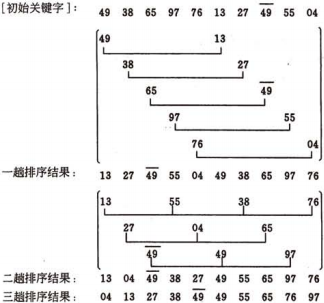
\includegraphics[width=240pt]{shellsort.png}\\
\figcaption{希尔排序}\label{fig:shellsort}
\end{center}

希尔排序的C语言实现如下。
\begin{Codex}[label=shell_sort.c]
/*
  * @brief 一趟希尔插入排序.
  *
  * 和一趟直接插入排序相比,仅有一点不同,就是前后元素的间距是gap而不是1
  *
  * @param[inout] a 待排序元素序列
  * @param[in] start 开始位置
  * @param[in] end 结束位置,最后一个元素后一个位置,即左闭右开区间
  * @param[in] gap 间隔
  * @return 无
  */
static void shell_insert(elem_t a[], const int start, const int end, const int gap) {
    elem_t tmp;
    int i, j;
    for (i = start + gap; i < end; i++) {
        tmp = a[i];
        for (j = i - gap; tmp < a[j] && j >= start; j -= gap) {
            a[j + gap] = a[j];
        }
        a[j + gap] = tmp;
    }
}

 /*
  * @brief 希尔排序.
  * @param[inout] a 待排序元素序列
  * @param[in] start 开始位置
  * @param[in] end 结束位置,最后一个元素后一个位置,即左闭右开区间
  * @return 无
  */
void shell_sort(elem_t a[], const int start, const int end) {
    int gap = end - start;
    while (gap > 1) {
        gap = gap / 3 + 1;
        shell_insert(a, start, end, gap);
    }
}
\end{Codex}


\section{交换排序} %%%%%%%%%%%%%%%%%%%%%%%%%%%%%%


\subsection{冒泡排序}
\textbf{冒泡排序}(Bubble Sort)的基本方法是:设待排序元素序列的元素个数为n,从后向前两两比较相邻元素的值,如果发生逆序(即前一个比后一个大),则交换它们,直到序列比较完。我们称它为一趟冒泡,结果是最小的元素交换到待排序序列的第一个位置,其他元素也都向排序的最终位置移动。下一趟冒泡时前一趟确定的最小元素不参加比较,待排序序列减少一个元素,一趟冒泡的结果又把序列中最小的元素交换到待排序序列的第一个位置。这样最多做n-1趟冒泡就能把所有元素排好序。

冒泡排序的C语言实现如下。
\begin{Codex}[label=bubble_sort.c]
/** 数组元素的类型 */
typedef int elem_t;

/**
  * @brief 冒泡排序.
  * @param[inout] a 待排序元素序列
  * @param[in] start 开始位置
  * @param[in] end 结束位置,最后一个元素后一个位置,即左闭右开区间
  * @return 无
  * @note 无
  * @remarks 无
  */
void bubble_sort(elem_t a[], const int start, const int end) {
    int exchange; /* 是否发生交换*/
    elem_t tmp;
    int i, j;

    for (i = start; i < end - 1; i++) {
        exchange = 0;
        for (j = end - 1; j > i; j--) { /* 发生逆序,交换*/
            if (a[j - 1] > a[j]) {
                tmp = a[j - 1];
                a[j - 1] = a[j];
                a[j] = tmp;
                exchange = 1;
            }
        }
        if (exchange == 0) return; /* 本趟无逆序,停止处理*/
    }
}
\end{Codex}

\subsection{快速排序}
\textbf{快速排序}(Quick sort)的基本思想是任取待排序元素序列中的某个元素(例如取第一个元素)作为基准,按照该元素的关键字大小,将整个元素序列划分为左右两个子序列:左侧子序列中所有元素的关键字都小于基准元素的关键字,右侧子序列中所有元素的关键字都大于或等于基准元素的关键字,基准元素则排在这两个子序列中间(这也是该元素最终应该安放的位置)。然后分别对这两个子序列重复施行上述算法,直到所有的元素都排在相应位置为止。

一趟快排的过程如图~\ref{fig:bubblesort} (a)所示。整个快速排序的过程可递归,如图~\ref{fig:bubblesort} (b)所示。

\begin{center}
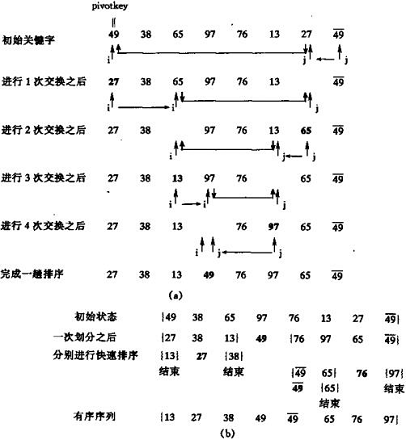
\includegraphics{bubblesort.png}\\
\figcaption{快速排序示例}\label{fig:bubblesort}
\end{center}

更多详细解释请参考本项目的wiki,\myurl{https://github.com/soulmachine/acm-cheatsheet/wiki/快速排序}

快速排序的C语言实现如下。
\begin{Codex}[label=quick_sort.c]
/** 数组元素的类型 */
typedef int elem_t;
 /*
  * @brief 一趟划分.
  * @param[inout] a 待排序元素序列
  * @param[in] start 开始位置
  * @param[in] end 结束位置,最后一个元素后一个位置,即左闭右开区间
  * @return 基准元素的新位置
  */
int partition(elem_t a[], const int start, const int end) {
    int i = start;
    int j = end - 1;
    const elem_t pivot = a[i];

    while(i < j) {
        while(i < j && a[j] >= pivot) j--;
        a[i] = a[j];
        while(i < j && a[i] <= pivot) i++;
        a[j] = a[i];
    }
    a[i] = pivot;
    return i;
}

/**
  * @brief 快速排序.
  * @param[inout] a 待排序元素序列
  * @param[in] start 开始位置
  * @param[in] end 结束位置,最后一个元素后一个位置
  * @return 无
  */
void quick_sort(elem_t a[], const int start, const int end) {
    if(start < end - 1) { /* 至少两个元素*/
        const int pivot_pos = partition(a, start, end);
        quick_sort(a, start, pivot_pos);
        quick_sort(a, pivot_pos + 1, end);
    }
}
\end{Codex}


\section{选择排序} %%%%%%%%%%%%%%%%%%%%%%%%%%%%%%
\textbf{选择排序}(Selection sort)的基本思想是:每一趟在后面n-i(i=1, 2, ..., n-2)个元素中选取最小的元素作为有序序列的第i个元素。


\subsection{简单选择排序}
\textbf{简单选择排序}(simple selection sort)也叫直接选择排序(straight selection sort),其基本步骤是:
\begindot
\item 在一组元素a[i]~a[n-1]中选择最小的元素;
\item 若它不是这组元素中的第一个元素,则将它与这组元素的第一个元素对调;
\item 在剩下的a[i+1]~a[n-1]中重复执行以上两步,直到剩余元素只有一个为止。
\myenddot

简单选择排序的C语言实现如下。
\begin{Codex}[label=simple_selection_sort.c]
/** 数组元素的类型 */
typedef int elem_t;

/**
  * @brief 简单选择排序.
  * @param[inout] a 待排序元素序列
  * @param[in] start 开始位置
  * @param[in] end 结束位置,最后一个元素后一个位置,即左闭右开区间
  * @return 无
  */
void simple_selection_sort(elem_t a[], int start, int end) {
    elem_t tmp;
    int i, j, k;

    for (i = start; i < end; i++) {
        k = i;
        /* 在a[i]到a[end-1]中寻找最小元素*/
        for (j = i + 1; j < end; j++)
            if(a[j] < a[k]) k = j;
        /* 交换*/
        if (k != i) {
            tmp = a[i];
            a[i] = a[k];
            a[k]= tmp;
        }
    }
}
\end{Codex}


\subsection{堆排序}
堆排序的C语言实现如下。
\begin{Codex}[label=heap_sort.c]
#include "heap.c"
/**
  * @brief 堆排序.
  * @param[inout] a 待排序元素序列
  * @param[in] n 元素个数
  * @param[in] cmp cmp 比较函数,小于返回-1,等于,大于
  * @return 无
  */
void heap_sort(heap_elem_t *a, const int n, 
               int (*cmp)(const heap_elem_t*, const heap_elem_t*)) {
    int i;
    heap_t *h;
    heap_elem_t tmp;

    h = heap_create(n, cmp);
    h->elems = a;

    i = (h->size - 2)/2;   /* 找最初调整位置:最后分支结点*/
    while (i >= 0) {  /* 自底向上逐步扩大形成堆*/
        heap_sift_down(h, i);
        i--;
    }

    for (i = h->size - 1; i > 0; i--) {
        tmp = h->elems[i];
        h->elems[i] = h->elems[0];
        h->elems[0] = tmp;
        h->size = i; /* 相当于h.size -- */
        heap_sift_down(h, 0);
    }
    heap_destroy(h);
}
\end{Codex}


\section{归并排序} %%%%%%%%%%%%%%%%%%%%%%%%%%%%%%
所谓“归并”,就是将两个或两个以上的有序序列合并成一个有序序列。我们先从最简单的二路\textbf{归并排序}(Merge sort)入手。

图~\ref{fig:mergesort}是一个二路归并排序的例子。

\begin{center}
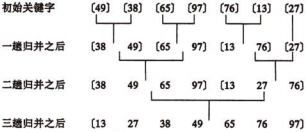
\includegraphics{mergesort.png}\\
\figcaption{二路归并排序示例}\label{fig:mergesort}
\end{center}

二路归并排序的C语言实现如下。
\begin{Codex}[label=merge_sort.c]
/** 数组元素的类型 */
typedef int elem_t;

 /** 数组元素的类型 */
typedef int elem_t;

 /*
  * @brief 将两个有序表合并成一个新的有序表
  * @param[inout] a 待排序元素序列,包含两个有序表
  * @param[in] tmp 与a等长的辅助数组
  * @param[in] start a[start]~a[mid-1]为第一个有序表
  * @param[in] mid 分界点
  * @param[in] end a[mid]~a[end-1]为第二个有序表
  * @return 无
  */
static void merge(elem_t a[], elem_t tmp[], const int start, 
        const int mid, const int end) {
    int i, j, k;
    for (i = 0; i < end; i++) tmp[i] = a[i];

    /* i, j是检测指针,k是存放指针*/
    for (i = start, j = mid, k = start; i < mid && j < end; k++) {
        if (tmp[i] < tmp[j]) {
            a[k] = tmp[i++];
        } else {
            a[k] = tmp[j++];
        }
    }
    /* 若第一个表未检测完,复制*/
    while (i < mid) a[k++] = tmp[i++];
    /* 若第二个表未检测完,复制*/
    while (j < end) a[k++] = tmp[j++];
}

/**
  * @brief 归并排序.
  * @param[inout] a 待排序元素序列
  * @param[in] tmp 与a等长的辅助数组
  * @param[in] start 开始位置
  * @param[in] end 结束位置,最后一个元素后一个位置,即左闭右开区间
  * @return 无
  * @note 无
  * @remarks 无
  */
void merge_sort(elem_t a[], elem_t tmp[], const int start, const int end) {
    if (start < end - 1) {
        const int mid = (start + end) / 2;
        merge_sort(a, tmp, start, mid);
        merge_sort(a, tmp, mid, end);
        merge(a, tmp, start, mid, end);
    }
}
\end{Codex}


\section{基数排序} %%%%%%%%%%%%%%%%%%%%%%%%%%%%%%
利用多关键字实现对单关键字排序的算法就称为\textbf{基数排序}(Radix sort)。

有两种顺序,最高位优先MSD(Most Significant Digit first)和最低位优先LSD(Least Significant Digit first)。

下面介绍“LSD链式基数排序”。首先以静态链表存储n个待排元素,并令表头指针指向第一个元素,即A[1]到A[n]存放元素,A[0]为表头结点,这样元素在重排时不必移动元素,只需要修改各个元素的link指针即可,如图~\ref{fig:radixsort}(a)所示。每个位设置一个桶(跟散列桶一样),桶采用静态链表结构,同时设置两个数组f[RADIX]和r[RADIX],记录每个桶的头指针和尾指针。排序过程就是d(关键字位数)趟“分配”、“收集”的过程,如图~\ref{fig:radixsort}所示。

\begin{center}
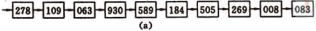
\includegraphics{radixsorta.png}\\
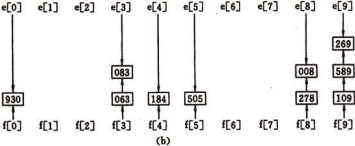
\includegraphics{radixsortb.png}\\
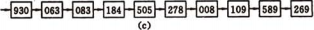
\includegraphics{radixsortc.png}\\
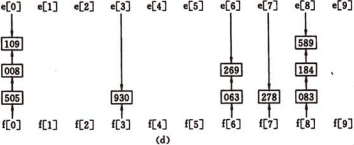
\includegraphics{radixsortd.png}\\
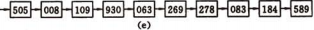
\includegraphics{radixsorte.png}\\
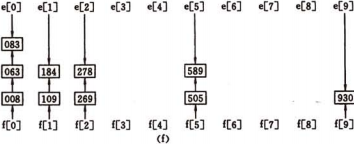
\includegraphics{radixsortf.png}\\
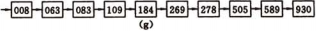
\includegraphics{radixsortg.png}\\
\figcaption{LSD链式基数排序示例}\label{fig:radixsort}
\end{center}

LSD链式基数排序的C语言实现如下。
\begin{Codex}[label=radix_sort.c]
/** @file radix_sort.c
  * @brief LSD链式基数排序.
  * @author soulmachine@gmail.com
  * @date 2013-05-18
  */
#include <stdio.h>  /* for printf() */

/* 关键字基数,此时是十进制*/
#define R 10  /*Radix*/

/**
  *@struct
  *@brief 静态链表结点.
  */
typedef struct static_list_node_t {
    int key; /** 关键字*/
    int link; /** 下一个节点*/
}static_list_node_t;

 /*
  * @brief 打印静态链表.
  * @param[in] a 静态链表数组
  * @return 无
  */
static void static_list_print(const static_list_node_t a[]) {
    int i = a[0].link;
    while (i != 0) {
        printf("%d ", a[i].key);
        i = a[i].link;
    }
}

 /*
  * @brief 获取十进制整数的某一位数字.
  * @param[in] n 整数
  * @param[in] i 第i位
  * @return 整数n第i位的数字
  */
static int get_digit(int n, const int i) {
    int j;
    for(j = 1; j < i; j++) {
        n /= 10;
    }

    return n % 10;
}

/**
  * @brief LSD链式基数排序.
  * @param[in] a 静态链表,a[0]是头指针
  * @param[in] n 待排序元素的个数
  * @param[in] d 最大整数的位数
  * @return 无
  * @note 无
  * @remarks 无
  */
void radix_sort(static_list_node_t a[], const int n, const int d) {
    int i, j, k, current, last;
    int rear[R], front[R];

    for(i = 0; i < n; i++) a[i].link = i + 1;
    a[n].link = 0;
    for(i = 0; i < d; i++) {
        /* 分配*/
        for(j = 0; j < R; j++) front[j] = 0;
        for(current = a[0].link; current != 0;
            current = a[current].link) {
            k = get_digit(a[current].key, i + 1);
            if(front[k] == 0) {
                front[k] = current;
                rear[k] = current;
            } else {
                a[rear[k]].link = current;
                rear[k] = current;
            }
        }

        /* 收集*/
        j = 0;
        while(front[j] == 0) j++;
        a[0].link = current = front[j];
        last = rear[j];
        for(j = j + 1; j < R; j++) {
            if(front[j] != 0) {
                a[last].link = front[j];
                last = rear[j];
            }
        }
        a[last].link = 0;
    }
}

void radix_sort_test(void) {
    static_list_node_t a[] = {{0,0}/* 头指针*/, {278,0}, {109,0}, 
    {63,0}, {930,0}, {589,0}, {184,0}, {505,0}, {269,0}, 
    {8,0}, {83,0}};
    radix_sort(a, 10, 3);
    static_list_print(a);
}
\end{Codex}


\section{总结和比较} %%%%%%%%%%%%%%%%%%%%%%%%%%%%%%

\begin{center}
\tabcaption{各种排序算法的总结和比较}

\vspace{1ex}
\begin{tabular}{lcccc}
\hline
\textbf{排序方法} & \textbf{平均时间} & \textbf{最坏情况} & \textbf{辅助存储} & \textbf{是否稳定}\\
\hline
直接插入排序 & $O(n^2)$ & $O(n^2)$ & $O(1)$ & 是\\
折半插入排序 & $O(n^2)$ & $O(n^2)$ & $O(1)$ & 是\\
希尔排序 & N/A & N/A & $O(1)$ & 否\\
冒泡排序 & $O(n^2)$ & $O(n^2)$ & $O(1)$ & 是\\
快速排序 & $O(n\log_2n)$ & $O(n^2)$ & $O(\log_2n)$ & 否\\
简单选择排序 & $O(n^2)$ & $O(n^2)$ & $O(1)$ & 否\\
堆排序 & $O(n\log_2n)$ & $O(n\log_2n)$ & $O(1)$ & 否\\
二路归并 & $O(n\log_2n)$ & $O(n\log_2n)$ & $O(n)$ & 是\\
基数排序 & $O(d\times (n+R))$ & $O(d\times (n+R))$ & $O(R)$ & 是\\
\hline
\end{tabular}
\end{center}

假设在数组中有两个元素$A_i,A_j,i<j$,即$A_i$在$A_j$之前,且$A_i=A_j$,如果在排序之后,$A_i$仍然在$A_j$的前面,则称这个排序算法是\textbf{稳定}的,否则称这个排序算法是\textbf{不稳定}的。

排序方法根据在排序过程中数据是否完全在内存,分为两大类:\textbf{内部排序}和\textbf{外部排序}。内部排序是指在排序期间数据全部存放在内存;外部排序是指在排序期间所有数据不能同时存放在内存,在排序过程中需要不断在内、外存之间交换。一般说到排序,默认是指内部排序。


\chapter{暴力枚举法}
暴力枚举法(brute force enumeration)又称为暴力搜索法(Brute-force search),详细定义见Wikipedia, \myurl{http://en.wikipedia.org/wiki/Brute_force_search}

\section{枚举排列} %%%%%%%%%%%%%%%%%%%%%%%%%%%%%%
枚举排列,即输出某个集合的所有排列。例如,集合{1,2,3}的所有排列是{(1,2,3),(1,3,2),(2,1,3),(2,3,1),(3,1,2),(3,2,1)}。

\subsection{生成1到n的全排列}

\subsubsection{描述}
给定一个正整数n,输出1到n的所有排列。

\subsubsection{分析}
我们尝试用递归的思路:先输出以1开头的排列(这一步是递归调用),然后输出以2开头的排列(又是递归调用),...,最后才是以n开头的排列。

以1开头的排列,第一位是1,后面是2到9的排列,这是一个子问题,可以接着递归。

伪代码如下:
\begin{Code}
void print_permutation(序列P,集合S) {
    if (S为空) 输出序列P
    else {
        for(按照从小到大的顺序依次考虑S中的每个元素e) {
            print_permutation(在A的末尾添加e后得到的新序列, S-{e});
        }
    }
}
// 调用
print_permutation({}, S);
\end{Code}

\subsubsection{代码}
下面考虑用C语言实现。不难想到用数组表示P和S。由于P和S是互补的,它们二者知道其中给一个,另一个就完全确定了,因此不用保存P。

C语言实现如下:

\begin{Codex}[label=print_permutation_n.c]
#include <stdio.h>
#include <stdlib.h>

/*
 * @brief 输出1到n的全排列
 * @param[in] n n
 * @param[in] cur 当前进行到哪个位置
 * @param[out] 存放一个排列
 * @return 无
 */
static void print_permutation_r(int n, int cur, int P[]) {
    int i, j;
    if (cur == n) { // 收敛条件
        for (i = 0; i < n; i++)
            printf("%d", P[i]);
        printf("\n");
    }

    // 扩展状态,尝试在A[cur]中填各种整数i,按从小到大的顺序
    for (i = 1; i <= n; i++) {
        int used = 0;
        for (j = 0; j < cur; j++)
            if (P[j] == i)
                used = 1; // 如果i已经在A[0]~A[cur-1]出现过,则不能再选
        if (!used) {
            P[cur] = i;
            print_permutation_r(n, cur + 1, P); // 递归调用
            // 不需要恢复P[cur],返回上层时时会被覆盖
        }
    }
}

/**
 * @brief 输出1到n的全排列
 * @param[in] n n
 * @return 无
 */
void print_permutation(int n) {
    int *P = (int*)malloc(n * sizeof(int));
    print_permutation_r(n, 0, P);
    free(P);
    return;
}

//test
int main() {
    print_permutation(3);
    return 0;
}
\end{Codex}


\subsection{生成可重集的排列}

\subsubsection{描述}
如果把问题改成,给定一个数组S,按字典序输出所有排列。

\subsubsection{分析}
此时S不再仅限于整数,可以是字符等。

首先想到可以利用上一题的思路,先输出1到n的全排列,然后把打印语句改成\fn{printf("\%c", S[P[i]-1])}即可。

但是这个方法有点问题,当集合中有重复元素时,它不能正确处理。例如S="AAA",它会打印出6个AAA。见下面的代码。

\begin{Code}
#include <stdio.h>
#include <stdlib.h>

/*
 * @brief 输出1到n的全排列,把数字当做下标
 * @param[in] S 字符集合
 * @param[in] n n
 * @param[in] cur 当前进行到哪个位置
 * @param[out] 存放一个排列
 * @return 无
 */
static void print_permutation_r(char S[], int n, int cur, int P[]) {
    int i, j;
    if (cur == n) { // 递归边界
        for (i = 0; i < n; i++)
            printf("%c", S[P[i]-1]);
        printf("\n");
    } else {
        // 尝试在A[cur]中填各种整数i,按从小到大的顺序
        for (i = 1; i <= n; i++) {
            int ok = 1;
            for (j = 0; j < cur; j++)
                if (P[j] == i)
                    ok = 0; // 如果i已经在A[0]~A[cur-1]出现过,则不能再选
            if (ok) {
                P[cur] = i;
                print_permutation_r(S, n, cur + 1, P); // 递归调用
            }
        }
    }
}

/**
 * @brief 输出字符集合的全排列
 * @param[in] S 字符集合
 * @param[in] n n
 * @return 无
 */
void print_permutation(char S[], int n) {
    int *P = (int*)malloc(n * sizeof(int));
    print_permutation_r(S, n, 0, P);
    free(P);
    return;
}

//test
int main() {
    char *S="ABC";
    char *S1="AAA";
    print_permutation(S,3);
    print_permutation(S1,3); // 不能正确处理可重集
    return 0;
}
\end{Code}

再换一个思路,还是在上一节的代码上进行修改,把\fn{if(P[j]==i)}和\fn{P[cur]=i}分别改成\fn{if(P[j]==S[i])}和\fn{P[cur]=S[i]}。这样,只要把S中的所有元素按从小到大的顺序排序,然后调用\fn{print_permutation_r(S, n, 0, P)}即可。

这个方法看上去不错,可惜还是有个小问题。例如\fn{S="AAA"},程序什么也不输出(正确答案应该是唯一的全排列AAA),原因在于,我们禁止S数组中出现重复,而在S中本来就有重复元素,这个“禁令”是错误的。

解决方法是,统计P[0]到P[cur-1]中S[i]出现的次数c1,以及S数组中S[i]的出现次数c2,只要c1<c2,就能继续选择S[i]。

结果又如何呢?这次有输出了,可是输出了27个AAA。遗漏是没有了,可是出现了重复。程序先把第1个A作为开头,递归调用结束后用第2个A作为开头,递归调用结束后用第3个A作为开头。每次输出3个排列,共27个。

枚举时应该\textbf{不重不漏}地取遍集合的所有元素。由于数组已经排序,所以只需要检查当前元素和前一个元素不相同,就可以做到不重不漏了。即只需要在\fn{for (i = 1; i <= n; i++)}和其后的花括号之间加上\fn{if(i==0 \&\& S[i] != S[i-1])}。见下面的代码。

\subsubsection{代码}

\begin{Codex}[label=print_permutation.c]
#include <stdio.h>
#include <stdlib.h>

/*
 * @brief 输出1到n的全排列
 * @param[in] n n
 * @param[in] cur 当前进行到哪个位置
 * @param[out] 存放一个排列
 * @return 无
 */
static void print_permutation_r(int n, int cur, int P[]) {
    int i, j;
    if (cur == n) { // 收敛条件
        for (i = 0; i < n; i++)
            printf("%d", P[i]);
        printf("\n");
    }

    // 扩展状态,尝试在A[cur]中填各种整数i,按从小到大的顺序
    for (i = 1; i <= n; i++) {
        int used = 0;
        for (j = 0; j < cur; j++) {
            if (P[j] == i) {
                used = 1; // 如果i已经在A[0]~A[cur-1]出现过,则不能再选
                break;
            }
        }
        if (!used) {
            P[cur] = i;
            print_permutation_r(n, cur + 1, P); // 递归调用
            // 不需要恢复P[cur],返回上层时时会被覆盖
        }
    }
}

/**
 * @brief 输出1到n的全排列
 * @param[in] n n
 * @return 无
 */
void print_permutation(int n) {
    int *P = (int*)malloc(n * sizeof(int));
    print_permutation_r(n, 0, P);
    free(P);
    return;
}

//test
int main() {
    print_permutation(3);
    return 0;
}
\end{Codex}


\subsection{下一个排列}
还可以利用STL中的\fn{next_permutation()},或者自己实现,见第 \S \ref{sec:nextpermutation}节的\fn{next_permutation()}。

\subsubsection{代码}

\begin{Codex}[label=print_permutation_next.c]
#include <stdio.h>
#include <stdlib.h>
#include <algorithm>

/**
 * @brief 输出字符集合的全排列,利用next_permutation
 * @param[in] S 字符集合
 * @param[in] n n
 * @return 无
 */
void print_permutation(char S[], int n) {
    sort(&S[0], &S[n]);
    do {
        for(int i = 0; i < n; i++) printf("%c", S[i]);
        printf("\n");
    }while(next_permutation(&S[0], &S[n]));
    return;
}

/* 等价于复制粘贴,这里为了节约篇幅,使用include,在OJ上提交时请用复制粘贴 */
#include "next_permutation.c"

/**
 * @brief 输出字符集合的全排列,利用第15章的next_permutation
 * @param[in] S 字符集合
 * @param[in] n n
 * @return 无
 */
void print_permutation1(char S[], int n) {
    sort(&S[0], &S[n]);
    int *N = (int*)malloc(n * sizeof(int));
    for (int i = 0; i < n; ++i) N[i]=S[i]-'A';
    do {
        for(int i = 0; i < n; i++) printf("%c", S[N[i]]);
        printf("\n");
    }while(next_permutation(&N[0], &N[n]));
    return;
}

//test
int main() {
    char S[]="ABC";
    char S1[]="AAA";
    print_permutation(S,3);
    print_permutation(S1,3);
    printf("\n\n");
    print_permutation1(S,3);
    print_permutation1(S1,3);
    return 0;
}
\end{Codex}


\section{子集生成} %%%%%%%%%%%%%%%%%%%%%%%%%%%%%%
给定一个集合,输出它所有的子集。为了简单起见,本节讨论的集合中没有重复元素。


\subsection{增量构造法}
一次选出一个元素,放或者不放到集合中。

\subsubsection{代码}

\begin{Codex}[label=subset.c]
#include <stdio.h>
#include <stdlib.h>

/**
 * @brief 增量构造法
 * @param[in] S 输入集合
 * @param[in] n 集合大小
 * @param[inout] P 某个子集
 * @param[in] cur p的当前位置
 * @param[in] ed S的当前位置,前面的元素已经选过了
 * @return 无
 */
void print_subset1(int *S, int n, int *P, int cur, int ed) {
    int i, j;
    for (i = ed; i < n; i++) {
        // 选择 S[i]
        P[cur] = S[i];
        for (j = 0; j <= cur; j++) printf("%d ", P[j]);
        printf("\n");
        // 不选择 S[i]
        print_subset1(S, n, P, cur + 1, i + 1);
    }
}
\end{Codex}


\subsection{位向量法}
开一个位向量B,B[i]=1表示选择S[i], B[i]=0表示不选择。

\subsubsection{代码}

\begin{Codex}[label=subset.c]
/**
 * @brief 位向量法
 * @param[in] S 输入集合
 * @param[in] n 集合大小
 * @param[in] B 位向量
 * @param[in] cur B的当前位置
 * @return 无
 */
void print_subset2(int *S, int n, char *B, int cur) {
    int i;
    if (cur == n) {
        for (i = 0; i < n; i++) if (B[i]) printf("%d ", S[i]);
        printf("\n");
        return;
    }
    B[cur] = 1;
    print_subset2(S, n, B, cur + 1);
    B[cur] = 0;
    print_subset2(S, n, B, cur + 1);
}
\end{Codex}


\subsection{二进制法}
前提:集合的元素不超过int位数。用一个int整数表示位向量,第i位为1,则表示选择S[i],为0则不选择。例如S=\{A,B,C,D\},则0110=6表示子集\{B,C\}。

这种方法最巧妙。因为它不仅能生成子集,还能方便的表示集合的并、交、差等集合运算。设两个集合的位向量分别为B1和B2,则B1|B2, B1\&B2, B1\^{}B2分别对应集合的并、交、对称差。

\subsubsection{代码}

\begin{Codex}[label=subset.c]
/**
 * @brief 二进制法
 * @param[in] S 输入集合
 * @param[in] n 集合大小
 * @param[in] B 位向量
 * @param[in] cur B的当前位置
 * @return 无
 */
void print_subset3(int *S, int n) {
    int i, j;
    for (i = 1; i < (1 << n); i++) {
        for (j = 0; j < n; j++)
            if (i & (1 << j)) printf("%d ", S[j]);
        printf("\n");
    }
}

int main() {
    int n, i;

    while(scanf("%d",&n) > 0) {
        int *S = (int*)malloc(n * sizeof(int));
        int *P = (int*)malloc(n * sizeof(int));
        char *B = (char*)malloc(n * sizeof(char));

        for(i = 0; i < n; i++) scanf("%d",&S[i]);

        print_subset1(S, n, P, 0, 0); putchar('\n');
        print_subset2(S, n, B, 0); putchar('\n');
        print_subset3(S, n);

        free(S);
        free(P);
        free(B);
    }
    return 0;
}
\end{Codex}


\section{Subsets} %%%%%%%%%%%%%%%%%%%%%%%%%%%%%%
\label{sec:subsets}


\subsubsection{描述}
Given a set of distinct integers, $S$, return all possible subsets.

Note:
\begindot
\item Elements in a subset must be in non-descending order.
\item The solution set must not contain duplicate subsets.
\myenddot

For example, If \code{S = [1,2,3]}, a solution is:
\begin{Code}
	[
	[3],
	[1],
	[2],
	[1,2,3],
	[1,3],
	[2,3],
	[1,2],
	[]
	]
\end{Code}


\subsection{递归}


\subsubsection{增量构造法}
每个元素,都有两种选择,选或者不选。

\begin{Code}
	// LeetCode, Subsets
	// 增量构造法,深搜,时间复杂度O(2^n),空间复杂度O(n)
	class Solution {
		public:
		vector<vector<int> > subsets(vector<int> &S) {
			sort(S.begin(), S.end());  // 输出要求有序
			vector<vector<int> > result;
			vector<int> path;
			subsets(S, path, 0, result);
			return result;
		}
		
		private:
		static void subsets(const vector<int> &S, vector<int> &path, int step,
		vector<vector<int> > &result) {
			if (step == S.size()) {
				result.push_back(path);
				return;
			}
			// 不选S[step]
			subsets(S, path, step + 1, result);
			// 选S[step]
			path.push_back(S[step]);
			subsets(S, path, step + 1, result);
			path.pop_back();
		}
	};
\end{Code}


\subsubsection{位向量法}
开一个位向量\fn{bool selected[n]},每个元素可以选或者不选。

\begin{Code}
	// LeetCode, Subsets
	// 位向量法,深搜,时间复杂度O(2^n),空间复杂度O(n)
	class Solution {
		public:
		vector<vector<int> > subsets(vector<int> &S) {
			sort(S.begin(), S.end());  // 输出要求有序
			
			vector<vector<int> > result;
			vector<bool> selected(S.size(), false);
			subsets(S, selected, 0, result);
			return result;
		}
		
		private:
		static void subsets(const vector<int> &S, vector<bool> &selected, int step,
		vector<vector<int> > &result) {
			if (step == S.size()) {
				vector<int> subset;
				for (int i = 0; i < S.size(); i++) {
					if (selected[i]) subset.push_back(S[i]);
				}
				result.push_back(subset);
				return;
			}
			// 不选S[step]
			selected[step] = false;
			subsets(S, selected, step + 1, result);
			// 选S[step]
			selected[step] = true;
			subsets(S, selected, step + 1, result);
		}
	};
\end{Code}


\subsection{迭代}


\subsubsection{增量构造法}
\begin{Code}
	// LeetCode, Subsets
	// 迭代版,时间复杂度O(2^n),空间复杂度O(1)
	class Solution {
		public:
		vector<vector<int> > subsets(vector<int> &S) {
			sort(S.begin(), S.end()); // 输出要求有序
			vector<vector<int> > result(1);
			for (auto elem : S) {
				result.reserve(result.size() * 2);
				auto half = result.begin() + result.size();
				copy(result.begin(), half, back_inserter(result));
				for_each(half, result.end(), [&elem](decltype(result[0]) &e){
					e.push_back(elem);
				});
			}
			return result;
		}
	};
\end{Code}


\subsubsection{二进制法}
本方法的前提是:集合的元素不超过int位数。用一个int整数表示位向量,第$i$位为1,则表示选择$S[i]$,为0则不选择。例如\fn{S=\{A,B,C,D\}},则\fn{0110=6}表示子集\fn{\{B,C\}}。

这种方法最巧妙。因为它不仅能生成子集,还能方便的表示集合的并、交、差等集合运算。设两个集合的位向量分别为$B_1$和$B_2$,则$B_1\cup B_2, B_1 \cap B_2, B_1 \triangle B_2$分别对应集合的并、交、对称差。

二进制法,也可以看做是位向量法,只不过更加优化。

\begin{Code}
	// LeetCode, Subsets
	// 二进制法,时间复杂度O(2^n),空间复杂度O(1)
	class Solution {
		public:
		vector<vector<int> > subsets(vector<int> &S) {
			sort(S.begin(), S.end()); // 输出要求有序
			vector<vector<int> > result;
			const size_t n = S.size();
			vector<int> v;
			
			for (size_t i = 0; i < 1 << n; i++) {
				for (size_t j = 0; j < n; j++) {
					if (i & 1 << j) v.push_back(S[j]);
				}
				result.push_back(v);
				v.clear();
			}
			return result;
		}
	};
\end{Code}


\subsubsection{相关题目}
\begindot
\item Subsets II,见 \S \ref{sec:subsets-ii}
\myenddot


\section{Subsets II} %%%%%%%%%%%%%%%%%%%%%%%%%%%%%%
\label{sec:subsets-ii}


\subsubsection{描述}
Given a collection of integers that might contain duplicates, $S$, return all possible subsets.

Note:

Elements in a subset must be in non-descending order.
The solution set must not contain duplicate subsets.
For example,
If \fn{S = [1,2,2]}, a solution is:
\begin{Code}
	[
	[2],
	[1],
	[1,2,2],
	[2,2],
	[1,2],
	[]
	]
\end{Code}


\subsubsection{分析}
这题有重复元素,但本质上,跟上一题很类似,上一题中元素没有重复,相当于每个元素只能选0或1次,这里扩充到了每个元素可以选0到若干次而已。


\subsection{递归}


\subsubsection{增量构造法}
\begin{Code}
	// LeetCode, Subsets II
	// 增量构造法,版本1,时间复杂度O(2^n),空间复杂度O(n)
	class Solution {
		public:
		vector<vector<int> > subsetsWithDup(vector<int> &S) {
			sort(S.begin(), S.end());  // 必须排序
			
			vector<vector<int> > result;
			vector<int> path;
			
			dfs(S, S.begin(), path, result);
			return result;
		}
		
		private:
		static void dfs(const vector<int> &S, vector<int>::iterator start,
		vector<int> &path, vector<vector<int> > &result) {
			result.push_back(path);
			
			for (auto i = start; i < S.end(); i++) {
				if (i != start && *i == *(i-1)) continue;
				path.push_back(*i);
				dfs(S, i + 1, path, result);
				path.pop_back();
			}
		}
	};
\end{Code}

\begin{Code}
	// LeetCode, Subsets II
	// 增量构造法,版本2,时间复杂度O(2^n),空间复杂度O(n)
	class Solution {
		public:
		vector<vector<int> > subsetsWithDup(vector<int> &S) {
			vector<vector<int> > result;
			sort(S.begin(), S.end()); // 必须排序
			
			unordered_map<int, int> count_map; // 记录每个元素的出现次数
			for_each(S.begin(), S.end(), [&count_map](int e) {
				if (count_map.find(e) != count_map.end())
				count_map[e]++;
				else
				count_map[e] = 1;
			});
			
			// 将map里的pair拷贝到一个vector里
			vector<pair<int, int> > elems;
			for_each(count_map.begin(), count_map.end(),
			[&elems](const pair<int, int> &e) {
				elems.push_back(e);
			});
			sort(elems.begin(), elems.end());
			vector<int> path; // 中间结果
			
			subsets(elems, 0, path, result);
			return result;
		}
		
		private:
		static void subsets(const vector<pair<int, int> > &elems,
		size_t step, vector<int> &path, vector<vector<int> > &result) {
			if (step == elems.size()) {
				result.push_back(path);
				return;
			}
			
			for (int i = 0; i <= elems[step].second; i++) {
				for (int j = 0; j < i; ++j) {
					path.push_back(elems[step].first);
				}
				subsets(elems, step + 1, path, result);
				for (int j = 0; j < i; ++j) {
					path.pop_back();
				}
			}
		}
	};
\end{Code}


\subsubsection{位向量法}
\begin{Code}
	// LeetCode, Subsets II
	// 位向量法,时间复杂度O(2^n),空间复杂度O(n)
	class Solution {
		public:
		vector<vector<int> > subsetsWithDup(vector<int> &S) {
			vector<vector<int> > result; // 必须排序
			sort(S.begin(), S.end());
			vector<int> count(S.back() - S.front() + 1, 0);
			// 计算所有元素的个数
			for (auto i : S) {
				count[i - S[0]]++;
			}
			
			// 每个元素选择了多少个
			vector<int> selected(S.back() - S.front() + 1, -1);
			
			subsets(S, count, selected, 0, result);
			return result;
		}
		
		private:
		static void subsets(const vector<int> &S, vector<int> &count,
		vector<int> &selected, size_t step, vector<vector<int> > &result) {
			if (step == count.size()) {
				vector<int> subset;
				for(size_t i = 0; i < selected.size(); i++) {
					for (int j = 0; j < selected[i]; j++) {
						subset.push_back(i+S[0]);
					}
				}
				result.push_back(subset);
				return;
			}
			
			for (int i = 0; i <= count[step]; i++) {
				selected[step] = i;
				subsets(S, count, selected, step + 1, result);
			}
		}
	};
\end{Code}


\subsection{迭代}


\subsubsection{增量构造法}
\begin{Code}
	// LeetCode, Subsets II
	// 增量构造法
	// 时间复杂度O(2^n),空间复杂度O(1)
	class Solution {
		public:
		vector<vector<int> > subsetsWithDup(vector<int> &S) {
			sort(S.begin(), S.end()); // 必须排序
			vector<vector<int> > result(1);
			
			size_t previous_size = 0;
			for (size_t i = 0; i < S.size(); ++i) {
				const size_t size = result.size();
				for (size_t j = 0; j < size; ++j) {
					if (i == 0 || S[i] != S[i-1] || j >= previous_size) {
						result.push_back(result[j]);
						result.back().push_back(S[i]);
					}
				}
				previous_size = size;
			}
			return result;
		}
	};
\end{Code}


\subsubsection{二进制法}
\begin{Code}
	// LeetCode, Subsets II
	// 二进制法,时间复杂度O(2^n),空间复杂度O(1)
	class Solution {
		public:
		vector<vector<int> > subsetsWithDup(vector<int> &S) {
			sort(S.begin(), S.end()); // 必须排序
			// 用 set 去重,不能用 unordered_set,因为输出要求有序
			set<vector<int> > result;
			const size_t n = S.size();
			vector<int> v;
			
			for (size_t i = 0; i < 1U << n; ++i) {
				for (size_t j = 0; j < n; ++j) {
					if (i & 1 << j)
					v.push_back(S[j]);
				}
				result.insert(v);
				v.clear();
			}
			vector<vector<int> > real_result;
			copy(result.begin(), result.end(), back_inserter(real_result));
			return real_result;
		}
	};
\end{Code}


\subsubsection{相关题目}
\begindot
\item Subsets,见 \S \ref{sec:subsets}
\myenddot


\section{Permutations} %%%%%%%%%%%%%%%%%%%%%%%%%%%%%%
\label{sec:permutations}


\subsubsection{描述}
Given a collection of numbers, return all possible permutations.

For example,
\fn{[1,2,3]} have the following permutations:
\fn{[1,2,3], [1,3,2], [2,1,3], [2,3,1], [3,1,2]}, and \fn{[3,2,1]}.


\subsection{next_permutation()}
偷懒的做法,可以直接使用\fn{std::next_permutation()}。如果是在OJ网站上,可以用这个API偷个懒;如果是在面试中,面试官肯定会让你重新实现。

\subsubsection{代码}
\begin{Code}
	// LeetCode, Permutations
	// 时间复杂度O(n!),空间复杂度O(1)
	class Solution {
		public:
		vector<vector<int> > permute(vector<int> &num) {
			vector<vector<int> > result;
			sort(num.begin(), num.end());
			
			do {
				result.push_back(num);
			} while(next_permutation(num.begin(), num.end()));
			return result;
		}
	};
\end{Code}


\subsection{重新实现next_permutation()}
见第 \S \ref{sec:next-permutation} 节。


\subsubsection{代码}
\begin{Code}
	// LeetCode, Permutations
	// 重新实现 next_permutation()
	// 时间复杂度O(n!),空间复杂度O(1)
	class Solution {
		public:
		vector<vector<int>> permute(vector<int>& num) {
			sort(num.begin(), num.end());
			
			vector<vector<int>> permutations;
			
			do {
				permutations.push_back(num);
			} while (next_permutation(num.begin(), num.end())); // 见第2.1节
			
			return permutations;
		}
	};
\end{Code}


\subsection{递归}
本题是求路径本身,求所有解,函数参数需要标记当前走到了哪步,还需要中间结果的引用,最终结果的引用。

扩展节点,每次从左到右,选一个没有出现过的元素。

本题不需要判重,因为状态装换图是一颗有层次的树。收敛条件是当前走到了最后一个元素。

\subsubsection{代码}
\begin{Code}
	// LeetCode, Permutations
	// 深搜,增量构造法
	// 时间复杂度O(n!),空间复杂度O(n)
	class Solution {
		public:
		vector<vector<int> > permute(vector<int>& num) {
			sort(num.begin(), num.end());
			
			vector<vector<int>> result;
			vector<int> path;  // 中间结果
			
			dfs(num, path, result);
			return result;
		}
		private:
		void dfs(const vector<int>& num, vector<int> &path,
		vector<vector<int> > &result) {
			if (path.size() == num.size()) {  // 收敛条件
				result.push_back(path);
				return;
			}
			
			// 扩展状态
			for (auto i : num) {
				// 查找 i 是否在path 中出现过
				auto pos = find(path.begin(), path.end(), i);
				
				if (pos == path.end()) {
					path.push_back(i);
					dfs(num, path, result);
					path.pop_back();
				}
			}
		}
	};
\end{Code}


\subsubsection{相关题目}
\begindot
\item Next Permutation, 见 \S \ref{sec:next-permutation}
\item Permutation Sequence, 见 \S \ref{sec:permutation-sequence}
\item Permutations II, 见 \S \ref{sec:permutations-ii}
\item Combinations, 见 \S \ref{sec:combinations}
\myenddot


\section{Permutations II} %%%%%%%%%%%%%%%%%%%%%%%%%%%%%%
\label{sec:permutations-ii}


\subsubsection{描述}
Given a collection of numbers that might contain duplicates, return all possible unique permutations.

For example,
\fn{[1,1,2]} have the following unique permutations:
\fn{[1,1,2], [1,2,1]}, and \fn{[2,1,1]}.


\subsection{next_permutation()}
直接使用\fn{std::next_permutation()},代码与上一题相同。


\subsection{重新实现next_permutation()}
重新实现\fn{std::next_permutation()},代码与上一题相同。


\subsection{递归}
递归函数\fn{permute()}的参数\fn{p},是中间结果,它的长度又能标记当前走到了哪一步,用于判断收敛条件。

扩展节点,每次从小到大,选一个没有被用光的元素,直到所有元素被用光。

本题不需要判重,因为状态装换图是一颗有层次的树。


\subsubsection{代码}
\begin{Code}
	// LeetCode, Permutations II
	// 深搜,时间复杂度O(n!),空间复杂度O(n)
	class Solution {
		public:
		vector<vector<int> > permuteUnique(vector<int>& num) {
			sort(num.begin(), num.end());
			
			unordered_map<int, int> count_map; // 记录每个元素的出现次数
			for_each(num.begin(), num.end(), [&count_map](int e) {
				if (count_map.find(e) != count_map.end())
				count_map[e]++;
				else
				count_map[e] = 1;
			});
			
			// 将map里的pair拷贝到一个vector里
			vector<pair<int, int> > elems;
			for_each(count_map.begin(), count_map.end(),
			[&elems](const pair<int, int> &e) {
				elems.push_back(e);
			});
			
			vector<vector<int>> result; // 最终结果
			vector<int> p;  // 中间结果
			
			n = num.size();
			permute(elems.begin(), elems.end(), p, result);
			return result;
		}
		
		private:
		size_t n;
		typedef vector<pair<int, int> >::const_iterator Iter;
		
		void permute(Iter first, Iter last, vector<int> &p,
		vector<vector<int> > &result) {
			if (n == p.size()) {  // 收敛条件
				result.push_back(p);
			}
			
			// 扩展状态
			for (auto i = first; i != last; i++) {
				int count = 0; // 统计 *i 在p中出现过多少次
				for (auto j = p.begin(); j != p.end(); j++) {
					if (i->first == *j) {
						count ++;
					}
				}
				if (count < i->second) {
					p.push_back(i->first);
					permute(first, last, p, result);
					p.pop_back(); // 撤销动作,返回上一层
				}
			}
		}
	};
\end{Code}


\subsubsection{相关题目}
\begindot
\item Next Permutation, 见 \S \ref{sec:next-permutation}
\item Permutation Sequence, 见 \S \ref{sec:permutation-sequence}
\item Permutations, 见 \S \ref{sec:permutations}
\item Combinations, 见 \S \ref{sec:combinations}
\myenddot


\section{Combinations} %%%%%%%%%%%%%%%%%%%%%%%%%%%%%%
\label{sec:combinations}


\subsubsection{描述}
Given two integers $n$ and $k$, return all possible combinations of $k$ numbers out of $1 ... n$.

For example,
If $n = 4$ and $k = 2$, a solution is:
\begin{Code}
	[
	[2,4],
	[3,4],
	[2,3],
	[1,2],
	[1,3],
	[1,4],
	]
\end{Code}


\subsection{递归}
\begin{Code}
	// LeetCode, Combinations
	// 深搜,递归
	// 时间复杂度O(n!),空间复杂度O(n)
	class Solution {
		public:
		vector<vector<int> > combine(int n, int k) {
			vector<vector<int> > result;
			vector<int> path;
			dfs(n, k, 1, 0, path, result);
			return result;
		}
		private:
		// start,开始的数, cur,已经选择的数目
		static void dfs(int n, int k, int start, int cur,
		vector<int> &path, vector<vector<int> > &result) {
			if (cur == k) {
				result.push_back(path);
			}
			for (int i = start; i <= n; ++i) {
				path.push_back(i);
				dfs(n, k, i + 1, cur + 1, path, result);
				path.pop_back();
			}
		}
	};
\end{Code}


\subsection{迭代}
\begin{Code}
	// LeetCode, Combinations
	// use prev_permutation()
	// 时间复杂度O((n-k)!),空间复杂度O(n)
	class Solution {
		public:
		vector<vector<int> > combine(int n, int k) {
			vector<int> values(n);
			iota(values.begin(), values.end(), 1);
			
			vector<bool> select(n, false);
			fill_n(select.begin(), k, true);
			
			vector<vector<int> > result;
			do{
				vector<int> one(k);
				for (int i = 0, index = 0; i < n; ++i)
				if (select[i])
				one[index++] = values[i];
				result.push_back(one);
			} while(prev_permutation(select.begin(), select.end()));
			return result;
		}
	};
\end{Code}


\subsubsection{相关题目}
\begindot
\item Next Permutation, 见 \S \ref{sec:next-permutation}
\item Permutation Sequence, 见 \S \ref{sec:permutation-sequence}
\item Permutations, 见 \S \ref{sec:permutations}
\item Permutations II, 见 \S \ref{sec:permutations-ii}
\myenddot


\section{Letter Combinations of a Phone Number } %%%%%%%%%%%%%%%%%%%%%%%%%%%%%%
\label{sec:letter-combinations-of-a-phone-number }


\subsubsection{描述}
Given a digit string, return all possible letter combinations that the number could represent.

A mapping of digit to letters (just like on the telephone buttons) is given below.

\begin{center}
	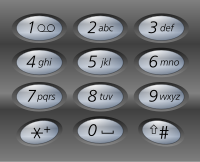
\includegraphics[width=150pt]{phone-keyboard.png}\\
	\figcaption{Phone Keyboard}\label{fig:phone-keyboard}
\end{center}

\textbf{Input:}Digit string \code{"23"}

\textbf{Output:} \code{["ad", "ae", "af", "bd", "be", "bf", "cd", "ce", "cf"]}.

\textbf{Note:}
Although the above answer is in lexicographical order, your answer could be in any order you want.


\subsubsection{分析}
无


\subsection{递归}
\begin{Code}
	// LeetCode, Letter Combinations of a Phone Number
	// 时间复杂度O(3^n),空间复杂度O(n)
	class Solution {
		public:
		const vector<string> keyboard { " ", "", "abc", "def", // '0','1','2',...
			"ghi", "jkl", "mno", "pqrs", "tuv", "wxyz" };
		
		vector<string> letterCombinations (const string &digits) {
			vector<string> result;
			dfs(digits, 0, "", result);
			return result;
		}
		
		void dfs(const string &digits, size_t cur, string path,
		vector<string> &result) {
			if (cur == digits.size()) {
				result.push_back(path);
				return;
			}
			for (auto c : keyboard[digits[cur] - '0']) {
				dfs(digits, cur + 1, path + c, result);
			}
		}
	};
\end{Code}


\subsection{迭代}
\begin{Code}
	// LeetCode, Letter Combinations of a Phone Number
	// 时间复杂度O(3^n),空间复杂度O(1)
	class Solution {
		public:
		const vector<string> keyboard { " ", "", "abc", "def", // '0','1','2',...
			"ghi", "jkl", "mno", "pqrs", "tuv", "wxyz" };
		
		vector<string> letterCombinations (const string &digits) {
			vector<string> result(1, "");
			for (auto d : digits) {
				const size_t n = result.size();
				const size_t m = keyboard[d - '0'].size();
				
				result.resize(n * m);
				for (size_t i = 0; i < m; ++i)
				copy(result.begin(), result.begin() + n, result.begin() + n * i);
				
				for (size_t i = 0; i < m; ++i) {
					auto begin = result.begin();
					for_each(begin + n * i, begin + n * (i+1), [&](string &s) {
						s += keyboard[d - '0'][i];
					});
				}
			}
			return result;
		}
	};
\end{Code}


\subsubsection{相关题目}
\begindot
\item 无
\myenddot

\chapter{广度优先搜索}
当题目看不出任何规律,既不能用分治,贪心,也不能用动规时,这时候万能方法——搜索,
就派上用场了。搜索分为广搜和深搜,广搜里面又有普通广搜,双向广搜,A*搜索等。
深搜里面又有普通深搜,回溯法等。

广搜和深搜非常类似(除了在扩展节点这部分不一样),二者有相同的框架,如何表示状态?
如何扩展状态?如何判重?尤其是判重,解决了这个问题,基本上整个问题就解决了。


\section{走迷宫} %%%%%%%%%%%%%%%%%%%%%%%%%%%%%%

\subsubsection{描述}
一个迷宫由一个01矩阵表示,每个单元格要么是空地(用0表示),要
么是障碍物(用1表示)。你的任务是找到一条从入口到出口的最短路径。任何时候都不能在障碍物格子中,也不
能走到迷宫之外。只能横着走或竖着走,不能斜着走。数据保证有唯一解。

\subsubsection{输入}
一个$5 \times 5$的二维数组

\subsubsection{输出}
左上角到右下角的最短路径

\subsubsection{样例输入}
\begin{Code}
0 1 0 0 0
0 1 0 1 0
0 0 0 0 0
0 1 1 1 0
0 0 0 1 0
\end{Code}

\subsubsection{样例输出}
(0, 0)
(1, 0)
(2, 0)
(2, 1)
(2, 2)
(2, 3)
(2, 4)
(3, 4)
(4, 4)

\subsubsection{分析}
既然求的是“最短”,很自然的思路是用BFS。举个例子,在如下图所示的迷宫中,假设
入口是左上角$(0,0)$,我们就从入口开始用BFS遍历迷宫,就可以算出从入口到
所有点的最短路径(如图~\ref{fig:maze}(a)所示),以及这些路径上每个节点的
前驱(如图~\ref{fig:maze}(b)所示)。

\begin{center}
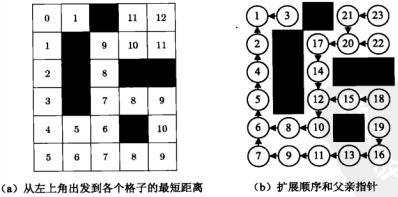
\includegraphics{maze.png}\\
\figcaption{用BFS求迷宫中最短路径}\label{fig:maze}
\end{center}

\subsubsection{代码}
\begin{Codex}[label=maze.c]
#include <stdio.h>
#include <string.h>

#define MAXN 5

// 迷宫的行数,列数
int m = MAXN, n = MAXN;
// 迷宫,0表示空地,1表示障碍物
int map[MAXN][MAXN];

// 四个方向
const char name[4] = { 'U', 'R', 'D', 'L' };
const int dx[4] = { -1, 0, 1, 0 }; // 行
const int dy[4] = { 0, 1, 0, -1 }; // 列

#ifndef __cplusplus
typedef char bool;
#define false 0
#define true 1
#endif

typedef struct state_t {
    int data;
    int action;
    int father;
} state_t;

#define STATE_MAX MAXN*MAXN  /* 状态总数 */

state_t nodes[STATE_MAX];

int state_hash(const state_t *s);

int state_index(const state *s) {
    return state_hash(s);
}

void print_action(const int end) {
    if (nodes[end].father == -1) return;

    print_action(nodes[end].father);
    putchar(name[nodes[end].action]);
}

void print_path(const int end) {
    if (nodes[end].father == -1) {
        printf("(%d, %d)\n", end / n, end % n);
        return;
    }
    print_path(nodes[end].father);
    printf("(%d, %d)\n", end / n, end % n);
}

void hashset_init();

bool hashset_find(const state_t *s);

void hashset_insert(const state_t *s);

void state_extend_init(const state_t *s);

bool state_extend(const state_t *s, state_t *next);

bool state_is_target(const state_t *s);

typedef state_t queue_elem_t; // 元素的类型
/* 等价于复制粘贴,这里为了节约篇幅,使用include,在OJ上提交时请用复制粘贴 */
#include "queue.c"  /* 见“栈和队列->队列”这节,如果是C++,则使用queue */

int bfs(state_t *start) {
    queue_t *q = queue_create(16);
    hashset_init();

    start->action = -1;
    start->father = -1;

    nodes[state_index(start)] = *start;
    hashset_insert(start);
    if (state_is_target(start))
        return state_index(start);
    queue_push(q, *start);

    while (!queue_empty(q)) {
        const state_t s = queue_front(q);
        queue_pop(q);
        state_t next;
        state_extend_init(&s);
        while (state_extend(&s, &next)) {
            if (state_is_target(&next)) {
                queue_destroy(q);
                return state_index(&next);
            }
            queue_push(q, next);
            hashset_insert(&next);
        }
    }
    queue_destroy(q);
    return -1;
}

int main(void) {
    int i, j;
    state_t start = {0, -1, -1}; /* 左上角为起点 */
    int end;

    for (i = 0; i < m; i++) {
        for (j = 0; j < n; j++) {
            scanf("%d", &map[i][j]);
        }
    }

    end = bfs(&start);
    print_path(end);
    return 0;
}

/********** functions implement **************/
/* 哈希表容量,要大于状态总数,若存在完美哈希方案,则等于状态总数 */
#define HASH_CAPACITY STATE_MAX
bool visited[HASH_CAPACITY];

int state_hash(const state_t *s) {
    return s->data;
}

void hashset_init() {
    memset(visited, 0, sizeof(visited));
}

bool hashset_find(const state_t *s) {
    return visited[state_hash(s)] == true;
}

void hashset_insert(const state_t *s) {
    visited[state_hash(s)] = true;
}

int action_cur;
#define ACTION_BEGIN 0
#define ACTION_END 4
/** 扩展点,即当前位置 */
int x, y;

void state_extend_init(const state_t *s) {
    action_cur = ACTION_BEGIN;
    x = s->data / n;
    y = s->data % n;
}

bool state_extend(const state_t *s, state_t *next) {
    while(action_cur < ACTION_END) {
        const int nx = x + dx[action_cur];
        const int ny = y + dy[action_cur];

        if (nx >= 0 && nx < m && ny >= 0 && ny < n && !map[nx][ny]) {
            next->data = nx * n + ny;

            if (!hashset_find(next)) { /* 判重 */
                /* 记录路径 */
                next->action = action_cur;
                next->father = state_index(s);
                nodes[state_index(next)] = *next;

                action_cur++;  /* return前别忘了增1 */
                return true;
            }
        }
        action_cur++;
    }
    return false;
}

const state_t END = {24, -1, -1};
bool state_is_target(const state_t *s) {
    return s->data == END.data;
}
\end{Codex}

\subsubsection{相关的题目}
与本题相同的题目:
\begindot
\item 《算法竞赛入门经典》\footnote{刘汝佳,算法竞赛入门经典,清华大学出版社,2009}第108页6.4.2节
\item  POJ 3984 迷宫问题, \myurl{http://poj.org/problem?id=3984}
\myenddot

与本题相似的题目:
\begindot
\item  POJ 2049 Finding Nemo, \myurl{http://poj.org/problem?id=2049}
\myenddot


\section{八数码问题} %%%%%%%%%%%%%%%%%%%%%%%%%%%%%%
\label{subsec:eightDigits}

\subsubsection{描述}
编号为1$\sim$8的8个正方形滑块摆成3行3列,有一个格子空着,如图~\ref{fig:eightDigits}所示。

\begin{center}
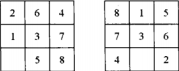
\includegraphics{eight-digits.png}\\
\figcaption{用BFS求迷宫中最短路径}\label{fig:eightDigits}
\end{center}

每次可以把与空格相邻的滑块(有公共边才算相邻)移到空格中,而它原
来的位置就成了新的空格。目标局面固定如下(用$x$表示空格):
\begin{Code}
1 2 3
4 5 6
7 8 x
\end{Code}

给定初始局面,计算出最短的移动路径。

\subsubsection{输入}
用一行表示一个局面,例如下面的这个局面:
\begin{Code}
 1  2  3
 x  4  6
 7  5  8
\end{Code}
可以表示为 1 2 3 x 4 6 7 5 8。 

\subsubsection{输出}
如果有解答,输出一个由四个字母'r','l','u','d'组成的移动路径。
如果没有,输出"unsolvable"。 

\subsubsection{样例输入}
\begin{Code}
2  3  4  1  5  x  7  6  8
\end{Code}

\subsubsection{样例输出}
\begin{Code}
ullddrurdllurdruldr
\end{Code}

\subsubsection{分析}
计算“最短”,很自然的想到BFS。

如何表示一个状态?一个3*3的棋盘,首先可以想到用一个数组\fn{int data[9]}来表示。把每个格子看做是整数的一位的话,可以用一个整数来表示,最大的棋盘87654321x,表示成整数就是876543210,没有超过32位整数的范围。

如何判重?用哈希表,自己实现或者用STL。C++ STL 里有\fn{set}, C++ 11新加入了\fn{unordered_set}。建议先用STL写一个版本,确保主算法正确,然后把\fn{set}(或\fn{unordered_set})替换成自己写的哈希表。

由于本题的特殊性,存在一种完美哈希(perfect hashing)方案。即\textbf{康托展开}。棋盘本身是一个排列,将排列转化为序数,用序数作为hash值。例如,1,2,3 这三个数字的全排列,按字典序,依次为
\begin{Code}
123 -- 0
132 -- 1
213 -- 2
231 -- 3
312 -- 4
321 -- 5
\end{Code}
其中,左侧为排列,右侧为其序数。

此题更优的解法还有双向BFS(见\S \ref{sec:biBFS}),A*算法(见\S \ref{sec:astar})。

\subsubsection{代码}

方案1,完美哈希,使用康托展开。

\begin{Codex}[label=eight_digits_bfs.c]
/* POJ 1077 Eight, http://poj.org/problem?id=1077 */
#include <stdio.h>
#include <string.h>

#define DIGITS 9 // 棋盘中数字的个数,也是变进制数需要的位数
#define     MATRIX_EDGE 3       // 棋盘边长

/***** 一些常量 *****/
const int SPACE_NUMBER = 0; // 空格对应着数字 0
// 上下左右四个方向
const int dx[] = {-1, 1, 0, 0};
const int dy[] = {0, 0, -1, 1};
const char name[] = { 'u', 'd', 'l', 'r' };

#ifndef __cplusplus
typedef char bool;
#define false 0
#define true 1
#endif

typedef char int8_t;

/**
 * @strut 状态
 */
typedef struct state_t {
    int8_t data[DIGITS];  /** 状态的数据. */
    int action; /* 由父状态移动到本状态的动作 */
    int father; /* 父状态在nodes[]中的下标,也即父状态的哈希值 */
    int count;  /** 所花费的步骤数(也即路径长度-1) */
} state_t;

// 3x3的棋盘,状态最多有 9!种
#define STATE_MAX 362880  /* 状态总数 */

state_t nodes[STATE_MAX+1];

int state_hash(const state_t *s);

int state_index(const state *s) {
    return state_hash(s);
}

/**
 * @brief 打印动作序列.
 * @param[in] end 终点状态的哈希值
 * @return 父状态
 */
void print_action(const int end) {
    if (nodes[end].father == -1) return;

    print_action(nodes[end].father);
    putchar(name[nodes[end].action]);
}

int state_hash(const state_t *s);

void hashset_init();

bool hashset_find(const state_t *s);

void hashset_insert(const state_t *s);

void state_extend_init(const state_t *s);

bool state_extend(const state_t *s, state_t *next);

bool state_is_target(const state_t *s);

typedef state_t queue_elem_t; // 元素的类型
/* 等价于复制粘贴,这里为了节约篇幅,使用include,在OJ上提交时请用复制粘贴 */
#include "queue.c"  /* 见“栈和队列->队列”这节,如果是C++,则使用queue */

int bfs(state_t *start) {
    queue_t *q = queue_create(16);
    hashset_init();

    start->action = -1;
    start->father = -1;
    start->count = 0;

    nodes[state_index(start)] = *start;
    hashset_insert(start);
    if (state_is_target(start))
        return state_index(start);
    queue_push(q, *start);

    while (!queue_empty(q)) {
        const state_t s = queue_front(q);
        state_t next;
        queue_pop(q);

        state_extend_init(&s);
        while (state_extend(&s, &next)) {
            if (state_is_target(&next)) {
                // printf("%d\n", next.count);
                queue_destroy(q);
                return state_index(&next);
            }
            queue_push(q, next);
            hashset_insert(&next);
        }
    }
    queue_destroy(q);
    return -1;
}

/**
 * @brief 输入.
 * @return 无
 */
void input(state_t *start) {
    int ch, i;
    for (i = 0; i < DIGITS; ++i) {
        do {
            ch = getchar();
        } while ((ch != EOF) && ((ch < '1') || (ch > '8')) && (ch != 'x'));
        if (ch == EOF) return;
        if (ch == 'x') start->data[i] = 0; // x 映射成数字 0
        else           start->data[i] = ch - '0';
    }
}

/** for wikioi 1225 */
void input1(state_t *start) {
    int i, n;
    scanf("%d", &n);

    /* 将整数转化为棋盘 */
    for(i = DIGITS-1; i >= 0; i--) {
        start->data[i] = n % 10;
        n /= 10;
    }
}

int main(void) {
    state_t start;
    int end; /* 目标状态在nodes[]中的下标 */
    input(&start);

    end = bfs(&start);

    print_action(end);
    printf("\n");
    return 0;
}

/********** functions implement **************/

/********** 方案1,完美哈希,使用康托展开 **************/

// 9 位变进制数(空格)能表示0到(9!-1)内的所有自然数,恰好有9!个,
// 与状态一一对应,因此可以把状态一一映射到一个9位变进制数

// 9 位变进制数,每个位数的单位,0!~8!
const int fac[] = {40320, 5040, 720, 120, 24, 6, 2, 1, 1};
/* 哈希表容量,要大于状态总数,若存在完美哈希方案,则等于状态总数 */
#define HASH_CAPACITY STATE_MAX

bool visited[HASH_CAPACITY];

int state_hash(const state_t *s) {
    int i, j;
    int key = 0;
    for (i = 0; i < DIGITS; i++) {
        int cnt = 0;  /* 逆序数 */
        for (j = i + 1; j < DIGITS; j++) if (s->data[i] > s->data[j]) cnt++;
        key += fac[i] * cnt;
    }
    return key;
}

void hashset_init() {
    memset(visited, 0, sizeof(visited));
}

bool hashset_find(const state_t *s) {
    return visited[state_hash(s)] == true;
}

void hashset_insert(const state_t *s) {
    visited[state_hash(s)] = true;
}

int action_cur;
#define ACTION_BEGIN 0
#define ACTION_END 4

/* 扩展点,即0的位置 */
int z;

void state_extend_init(const state_t *s) {
    action_cur = ACTION_BEGIN;
    for (z = 0; z < DIGITS; z++) {
        if (s->data[z] == SPACE_NUMBER) {
            break;  // 找 0 的位置
        }
    }
}

bool state_extend(const state_t *s, state_t *next) {
    const int x = z / MATRIX_EDGE; // 行
    const int y = z % MATRIX_EDGE; // 列

    while (action_cur < ACTION_END) {
        const int newx = x + dx[action_cur];
        const int newy = y + dy[action_cur];
        const int newz = newx * MATRIX_EDGE + newy;

        if (newx >= 0 && newx < MATRIX_EDGE && newy >= 0 &&
                newy < MATRIX_EDGE) { // 没有越界
            *next = *s;
            next->data[newz] = SPACE_NUMBER;
            next->data[z] = s->data[newz];
            next->count = s->count + 1;
            if (!hashset_find(next)) { /* 判重 */
                next->action = action_cur;
                next->father = state_index(s);
                /* 记录路径 */
                nodes[state_index(next)] = *next;
                action_cur++; /* return前别忘了增1 */
                return true;
            }
        }
        action_cur++;
    }
    return false;
}

// 目标状态
const state_t END = {{1, 2, 3, 4, 5, 6, 7, 8, 0}, -1, -1};
// for wikioi 1225
const state_t END1 = {{1, 2, 3, 8, 0, 4, 7, 6, 5}, -1, -1};

bool state_is_target(const state_t *s) {
    return memcmp(s->data, END.data, DIGITS * sizeof(int8_t)) == 0;
}
\end{Codex}

方案2,不知道是否存在完美哈希方案,但能够预估状态个数的上限,用树双亲表示法存储路径,用自己实现的哈希表判重。

\begin{Codex}[label=eight_digits_bfs2.c]
/* POJ 1077 Eight, http://poj.org/problem?id=1077 */
#include <stdio.h>
#include <string.h>
#include <assert.h>

#define DIGITS 9 // 棋盘中数字的个数,也是变进制数需要的位数
#define     MATRIX_EDGE 3       // 棋盘边长

/***** 一些常量 *****/
const int SPACE_NUMBER = 0; // 空格对应着数字 0
// 上下左右四个方向
const int dx[] = {-1, 1, 0, 0};
const int dy[] = {0, 0, -1, 1};
const char name[] = { 'u', 'd', 'l', 'r' };

#ifndef __cplusplus
typedef char bool;
#define false 0
#define true 1
#endif

typedef char int8_t;

/**
 * @strut 状态
 */
typedef struct state_t {
    int8_t data[DIGITS];  /** 状态的数据. */
    int action; /* 由父状态移动到本状态的动作 */
    int index;  /** 本状态在nodes[]中的下标 */
    int father; /** 父状态在nodes[]中的下标 */
    int count;  /** 所花费的步骤数(也即路径长度-1) */
} state_t;

// 3x3的棋盘,状态最多有 9!种
#define STATE_MAX 362880  /* 状态总数 */

state_t nodes[STATE_MAX+1];
int path_index = 0;

int state_index(const state_t *s) {
    return s->index;
}

/**
 * @brief 打印动作序列.
 * @param[in] end 终点状态的哈希值
 * @return 父状态
 */
void print_action(const int end) {
    if (nodes[end].father == -1) return;

    print_action(nodes[end].father);
    putchar(name[nodes[end].action]);
}

void hashset_init();

bool hashset_find(const state_t *s);

void hashset_insert(const state_t *s);

void state_extend_init(const state_t *s);

bool state_extend(const state_t *s, state_t *next);

bool state_is_target(const state_t *s);

typedef state_t queue_elem_t; // 元素的类型
/* 等价于复制粘贴,这里为了节约篇幅,使用include,在OJ上提交时请用复制粘贴 */
#include "queue.c"  /* 见“栈和队列->队列”这节,如果是C++,则使用queue */

int bfs(state_t *start) {
    queue_t *q = queue_create(16);
    hashset_init();

    start->action = -1;
    start->index = path_index++;
    start->father = -1;
    start->count = 0;

    nodes[state_index(start)] = *start;
    hashset_insert(start);
    if (state_is_target(start))
        return state_index(start);
    queue_push(q, *start);

    while (!queue_empty(q)) {
        const state_t s = queue_front(q);
        state_t next;
        queue_pop(q);

        state_extend_init(&s);
        while (state_extend(&s, &next)) {
            if (state_is_target(&next)) {
                // printf("%d\n", next.count);
                queue_destroy(q);
                return state_index(next);
            }
            queue_push(q, next);
            hashset_insert(&next);
        }
    }
    queue_destroy(q);
    return -1;
}

/**
 * @brief 输入.
 * @return 无
 */
void input(state_t *start) {
    int ch, i;
    for (i = 0; i < DIGITS; ++i) {
        do {
            ch = getchar();
        } while ((ch != EOF) && ((ch < '1') || (ch > '8')) && (ch != 'x'));
        if (ch == EOF) return;
        if (ch == 'x') start->data[i] = 0; // x 映射成数字 0
        else           start->data[i] = ch - '0';
    }
}

/** for wikioi 1225 */
void input1(state_t *start) {
    int i, n;
    scanf("%d", &n);

    /* 将整数转化为棋盘 */
    for(i = DIGITS-1; i >= 0; i--) {
        start->data[i] = n % 10;
        n /= 10;
    }
}

int main(void) {
    state_t start;
    int end;
    input(&start);

    end = bfs(&start);

    print_action(end);
    printf("\n");
    return 0;
}

/********** functions implement **************/

/********** 方案2 不知道完美哈希方案,自己实现哈希表 **************/
#define HASH_CAPACITY  10000000  /* 哈希表容量,要大于状态总数 */

int head[HASH_CAPACITY];
int next[STATE_MAX];

int state_hash(const state_t *s) {
    int i;
    int ret = 0;
    for(i = 0; i < DIGITS; i++) ret = ret * 10 + s->data[i];
    return ret % HASH_CAPACITY;
}

void hashset_init() {
    memset(head, 0, sizeof(head));
    memset(next, 0, sizeof(next));
}

bool hashset_find(const state_t *s) {
    const int h = state_hash(s);
    int u = head[h]; // 从表头开始查找单链表
    while(u) {
        // 找到了
        if(memcmp(nodes[u].data, s->data,
                DIGITS * sizeof(int8_t)) == 0) return true;
        u = next[u]; // 顺着链表继续找
    }
    return false;
}

void hashset_insert(const state_t *s) {
    const int h = state_hash(s);
    int u = head[h]; // 从表头开始查找单链表
    while(u) {
        // 找到了,插入失败
        if(memcmp(nodes[u].data, nodes[s->index].data,
                sizeof(DIGITS * sizeof(int8_t))) == 0) return;
        u = next[u]; // 顺着链表继续找
    }
    assert(head[h] >= 0);
    next[s->index] = head[h];  /* 插入到首节点前面,头查法 */
    head[h] = s->index;
    return;
}

int action_cur;
#define ACTION_BEGIN 0
#define ACTION_END 4

/* 扩展点,即0的位置 */
int z;

void state_extend_init(const state_t *s) {
    action_cur = ACTION_BEGIN;
    for (z = 0; z < DIGITS; z++) {
        if (s->data[z] == SPACE_NUMBER) {
            break;  // 找 0 的位置
        }
    }
}

bool state_extend(const state_t *s, state_t *next) {
    const int x = z / MATRIX_EDGE; // 行
    const int y = z % MATRIX_EDGE; // 列

    while (action_cur < ACTION_END) {
        const int newx = x + dx[action_cur];
        const int newy = y + dy[action_cur];
        const int newz = newx * MATRIX_EDGE + newy;

        next->count = s->count + 1;
        if (newx >= 0 && newx < MATRIX_EDGE && newy >= 0 &&
                newy < MATRIX_EDGE) { // 没有越界
            *next = *s;
            next->data[newz] = SPACE_NUMBER;
            next->data[z] = s->data[newz];

            if (!hashset_find(next)) { /* 判重 */
                next->action = action_cur;
                next->index = path_index++;
                next->father = state_index(s);
                /* 记录路径 */
                nodes[state_index(next)] = *next;
                action_cur++; /* return前别忘了增1 */
                return true;
            }
        }
        action_cur++;
    }
    return false;
}

// 目标状态
const state_t END = {{1, 2, 3, 4, 5, 6, 7, 8, 0}, -1, -1};
// for wikioi 1225
const state_t END1 = {{1, 2, 3, 8, 0, 4, 7, 6, 5}, -1, -1};

bool state_is_target(const state_t *s) {
    return memcmp(s->data, END.data, DIGITS * sizeof(int8_t)) == 0;
}
\end{Codex}

方案3,不知道完美哈希方案,但能够预估状态个数的上限制,用树双亲表示法存储路径,用标准库的哈希表判重。

\begin{Codex}[label=eight_digits_bfs3.cpp]
//前面的代码与方案2一摸一样
//...

/********** 方案3 不知道完美哈希方案,使用标准库的哈希表 **************/

// 重载 state_t 的 == 操作符
typedef struct state_t {
    int8_t data[DIGITS];  /** 状态的数据. */
    int action; /* 由父状态移动到本状态的动作 */
    int index;  /** 本状态在nodes[]中的下标 */
    int father; /** 父状态在nodes[]中的下标 */
    int count;  /** 所花费的步骤数(也即路径长度-1) */

    bool operator==(const state_t& other) const {
        return memcmp(data, other.data, DIGITS * sizeof(int8_t)) == 0;
    }
} state_t;

#include <unordered_set>

// 定制一个哈希函数
namespace std {
template<> struct hash<state_t> {
    size_t operator()(const state_t & x) const {
        int i;
        int ret = 0;
        for (i = 0; i < DIGITS; i++)
            ret = ret * 10 + x.data[i];
        return ret;
    }
};
}

unordered_set<state_t> visited;

void hashset_init() {
    visited.clear();
}

bool hashset_find(const state_t *s) {
    return visited.count(*s) > 0;
}

void hashset_insert(const state_t *s) {
    visited.insert(*s);
}

//...
//后面的代码也与方案2一摸一样
\end{Codex}

\subsubsection{相关的题目}
与本题相同的题目:
\begindot
\item 《算法竞赛入门经典》\footnote{刘汝佳,算法竞赛入门经典,清华大学出版社,2009} 第131页7.5.3节
\item  POJ 1077 Eight, \myurl{http://poj.org/problem?id=1077}
\item  wikioi 1225 八数码难题, \myurl{http://www.wikioi.com/problem/1225/}
\myenddot

与本题相似的题目:
\begindot
\item  POJ 2893 M × N Puzzle, \myurl{http://poj.org/problem?id=2893}
\myenddot


\section{四子连棋} %%%%%%%%%%%%%%%%%%%%%%%%%%%%%%

\subsubsection{描述}
在一个4*4的棋盘上摆放了14颗棋子,其中有7颗白色棋子,7颗黑色棋子,有两个空白地带,任何一颗黑白
棋子都可以向上下左右四个方向移动到相邻的空格,这叫行棋一步,黑白双方交替走棋,任意一方可以先走,
如果某个时刻使得任意一种颜色的棋子形成四个一线(包括斜线),这样的状态为目标棋局。

\subsubsection{输入}
一个4*4的初始棋局,黑棋子用B表示,白棋子用W表示,空格地带用O表示。

\subsubsection{输出}
移动到目标棋局的最少步数。

\subsubsection{样例输入}
\begin{Code}
BWBO
WBWB
BWBW
WBWO
\end{Code}

\subsubsection{样例输出}
\begin{Code}
5
\end{Code}

\subsubsection{分析}
求最少步数,很自然的想到广搜。

如何表示一个状态?用一个二维数组\fn{int board[4][4]}表示,还需要记录该状态是由白子还是黑子移动而导致的,走到该状态已经花费的步数。

如何扩展节点?每一步,从队列弹出一个状态,两个空格都可以向四个方向扩展,把得到的状态入队列。

如何判重?棋盘用二维矩阵存储,用0表示空格,1表示黑色,2表示白色,所以最后可以看成一个16位的三进制数。
用这个数作为棋盘的编码,就可以用来判重了。注意,本题要黑白交替走,所以我们要区分状态是由白子还是黑子移动而导致的。

可以用C++的\fn{map}来判重,
\begin{Code}
/* visited[0]记录白子的历史, visited[1]记录黑子的历史. */
map<int, bool> visited[2];
\end{Code}

也可以开一个大数组当做哈希表,
\begin{Code}
#define HASH_MOD 43036875 /* hash表大小 */
/* visited[0]记录白子的历史, visited[1]记录黑子的历史. */
bool visited[2][HASH_MOD];
\end{Code}

\subsubsection{代码}
\begin{Codex}[label=four_adjacent.c]
/** wikioi 1004 四子连棋  , http://www.wikioi.com/problem/1004 */
#include <stdio.h>
#include <string.h>

#define LEN 4   /* 边长 */

/* 右,左,上,下(左下角为坐标原点)*/
const int dx[] = { 1, -1, 0, 0 };
const int dy[] = { 0, 0, 1, -1 };


#ifndef __cplusplus
typedef char bool;
#define false 0
#define true 1
#endif

/**
 * @strut 状态
 */
typedef struct state_t {
    // 状态的数据
    int board[LEN][LEN]; /* 棋局,1表示黑子,2表示白子,0表示空白 */
    int color; /* 本状态是由白子还是黑子移动而导致的 */
    int count;  /** 所花费的步骤数(也即路径长度-1),求路径长度时需要 */
} state_t;

/**
 * @brief 计算状态的哈希值。
 * 棋盘用二维矩阵存储,用0表示空格,1表示黑色,2表示白色,所以最后可以看成
 * 一个16位的三进制数。最大为
 * 2222
 * 2221
 * 1111
 * 1100
 * 值为 43036875。
 * @return 棋盘所表示的三进制数转化为十进制数
 */
//TODO:共C16 7×C9 2个状态,用类似康托的方法储存
int state_hash(const state_t *s);

void hashset_init();

bool hashset_find(const state_t *s);

void hashset_insert(const state_t *s);

void state_extend_init(const state_t *s);

bool state_extend(const state_t *s, state_t *next);

bool state_is_target(const state_t *s);

typedef state_t queue_elem_t; // 元素的类型
/* 等价于复制粘贴,这里为了节约篇幅,使用include,在OJ上提交时请用复制粘贴 */
#include "queue.c"  /* 见“栈和队列->队列”这节,如果是C++,则使用queue */

void bfs(state_t *start) {
    queue_t *q = queue_create(16);
    hashset_init();

    start->count = 0;
    start->color = 1;

    hashset_insert(start);
    queue_push(q, *start);

    start->color = 2;

    hashset_insert(start); // 千万别忘记了标记此处的访问记录
    if (state_is_target(start)) /* 如果起点就是终点,返回 */
        return;
    queue_push(q, *start);

    while (!queue_empty(q)) {
        const state_t s = queue_front(q);
        state_t next;
        queue_pop(q);

        state_extend_init(&s);
        while (state_extend(&s, &next)) {
            if (state_is_target(&next)) {
                printf("%d\n", next.count);
                queue_destroy(q);
                return;
            }
            queue_push(q, next);
            hashset_insert(&next);
        }
    }
    queue_destroy(q);
}

int main() {
    int i, j;
    char s[LEN + 1];
    state_t start;

    for (i = 0; i < LEN; i++) {
        scanf("%s", s);
        for (j = 0; j < LEN; j++) {
            if (s[j] == 'B') start.board[i][j] = 1;
            else if (s[j] == 'W') start.board[i][j] = 2;
            else start.board[i][j] = 0;
        }
    }

    bfs(&start);
    queue_destroy(q);
    return 0;
}

/************ functions implement ************/

/* 哈希表容量,要大于状态总数,若存在完美哈希方案,则等于状态总数 */
#define HASH_CAPACITY 43036875

/** 哈希表,标记状态是否已访问过。
 * visited[0]记录白子的历史,visited[1]记录黑子的历史.
 */
bool visited[2][HASH_CAPACITY];

#define RADIX 3 /* 三进制 */

int state_hash(const state_t *s) {
    int i, j;
    int ret = 0;

    for (i = 0; i < LEN; i++) {
        for (j = 0; j < LEN; j++) {
            ret = ret * RADIX + s->board[i][j];
        }
    }
    return ret;
}

void hashset_init() {
    memset(visited[0], 0, sizeof(sizeof(bool) * HASH_CAPACITY));
    memset(visited[1], 0, sizeof(sizeof(bool) * HASH_CAPACITY));
}

bool hashset_find(const state_t *s) {
    return visited[s->color - 1][state_hash(s)] == true;
}

void hashset_insert(const state_t *s) {
    visited[s->color - 1][state_hash(s)] = true;
}

/* 扩展的时候,先定空格,再定方向 */
/* 记录当前方向,例如action_cur[0]记录了第一个空格,当前在扩展哪个方向
 */
int action_cur[2];
#define ACTION_BEGIN 0
#define ACTION_END 4

typedef struct point_t {
    int x, y;
} point_t;

/* 记录当前在扩展哪一个空格,值为0或1 */
int space_cur;
/* 两个空格的位置 */
point_t extend_pos[2];

void state_extend_init(const state_t *s) {
    int i, j, k;
    action_cur[0] = ACTION_BEGIN;
    action_cur[1] = ACTION_BEGIN;
    space_cur = 0;

    k = 0;
    // 寻找两个空白的格子的位置
    for (i = 0; i < LEN; i++) {
        for (j = 0; j < LEN; j++) {
            if (s->board[i][j] == 0) {
                extend_pos[k].x = i;
                extend_pos[k].y = j;
                k++;
            }
        }
    }
}

bool state_extend(const state_t *s, state_t *next) {
    int i;

    for (i = 0; i < 2; i++) { /* 先第一个空格,再第二个空格 */
        while (action_cur[i] < ACTION_END) {
            const int x = extend_pos[i].x;
            const int y = extend_pos[i].y;
            int nextx = x + dx[action_cur[i]];
            int nexty = y + dy[action_cur[i]];
            *next = *s;
            next->count = s->count + 1;
            next->color = 3 - s->color;

            if (nextx >= 0 && nextx < LEN && nexty >= 0 && nexty < LEN
                    /* 必须黑白交替走 */
                    && next->color == s->board[nextx][nexty]) {
                /* swap */
                {
                    int temp = next->board[x][y];
                    next->board[x][y] = next->board[nextx][nexty];
                    next->board[nextx][nexty] = temp;
                }

                if (!hashset_find(next)) { /* 判重 */
                    action_cur[i]++; /* return前别忘了增1 */
                    return true;
                }
            }
            action_cur[i]++;
        }
    }
    return false;
}

bool state_is_target(const state_t *s) {
    int i, j;
    for (i = 0; i < LEN; i++) {  /* 逐行检查 */
        int flag = 1;  /* 某一行全是同一颜色 */
        for (j = 1; j < LEN; j++)
            if (s->board[i][j - 1] != s->board[i][j])
                flag = 0;
        if (flag)
            return 1;
    }
    for (j = 0; j < LEN; j++) { //逐列检查
        int flag = 1;  /* 某一行全是同一颜色 */
        for (i = 1; i < LEN; i++)
            if (s->board[i][j] != s->board[i - 1][j]) flag = 0;
        if (flag) return 1;
    }
    /* 斜线 */
    if (s->board[0][0] == s->board[1][1] && s->board[1][1] == s->board[2][2]
            && s->board[2][2] == s->board[3][3])
        return 1;
    if (s->board[0][3] == s->board[1][2] && s->board[1][2] == s->board[2][1]
            && s->board[2][1] == s->board[3][0])
        return 1;
    return 0;
}
\end{Codex}

\subsubsection{相关的题目}
与本题相同的题目:
\begindot
\item  wikioi 1004 四子连棋, \myurl{http://www.wikioi.com/problem/1004/}
\myenddot

与本题相似的题目:
\begindot
\item  None
\myenddot


\section{双向BFS} %%%%%%%%%%%%%%%%%%%%%%%%%%%%%%
\label{sec:biBFS}


\subsection{八数码问题}
题目见 \S \ref{subsec:eightDigits}。

\subsubsection{代码}

\begin{Codex}[label=eight_digits_bibfs.c]

\end{Codex}


\section{A*算法} %%%%%%%%%%%%%%%%%%%%%%%%%%%%%%
\label{sec:astar}

\textbf{A*算法 = 宽搜 + 优先队列}

将广搜模板(见第\S \ref{sec:bfs-template}节)中的队列改为优先队列,设计好当前状态距离目标状态的预估距离$h()$,就变成了A*算法!

\subsection{八数码问题}
题目见 \S \ref{subsec:eightDigits}。

\subsubsection{代码}
\begin{Codex}[label=eight_digits_astar.c]
/** POJ 1077 Eight, http://poj.org/problem?id=1077
 简单解释几个要点,便于理解代码.
1. 怎么判断是否有解?只要计算出的逆序个数总和为奇数,该数据必然无解
2. 如何判断某一状态是否到过?本题存在一种完美哈希方案,即用康托展开。
        详见 http://128kj.iteye.com/blog/1699795
3.使用优先队列,即堆,加速挑选最优值。
4.函数 g=此状态在搜索树中已经走过的路径的节点数.
5.估价函数 h ,采用曼哈顿距离, 见代码 calcH 函数。曼哈顿距离的定义是,
 假设有两个点(x1,y1),(x2,y2),则曼哈顿距离L1=|x1-x2| + |y1-y2|
 */
#include <stdio.h>
#include <string.h>

#define DIGITS 9 // 棋盘中数字的个数,也是变进制数需要的位数
#define     MATRIX_EDGE 3       // 棋盘边长
#define RADIX 10

/***** 一些常量 *****/
const int SPACE_NUMBER = 0; // 空格对应着数字 0
// 上下左右四个方向
const int dx[] = {-1, 1, 0, 0};
const int dy[] = {0, 0, -1, 1};
const char name[] = { 'u', 'd', 'l', 'r' };

// 目标状态
const int GOAL = 123456780;
// 每个数字在棋盘中的位置,例如0,在(2,2)=8这个位置上
int GOAL_POS[DIGITS];

#ifndef __cplusplus
typedef char bool;
#define false 0
#define true 1
#endif

/**
 * @strut 状态
 */
typedef struct state_t {
    int board;  /** 状态的数据,即棋局. */
    int action; /* 由父状态移动到本状态的动作 */
    int father; /* 父状态在nodes[]中的下标,也即父状态的哈希值 */
    int count;  /** 所花费的步骤数(也即路径长度-1),作为g */
    int h; /** 距离目标状态的估算距离 */
} state_t;

// 3x3的棋盘,状态最多有 9!种
#define STATE_MAX 362880  /* 状态总数 */

state_t nodes[STATE_MAX+1];

int state_hash(const state_t *s);

int state_index(const state_t *s) {
    return state_hash(s);
}
/**
 * @brief 打印动作序列.
 * @param[in] end 终点状态的哈希值
 * @return 父状态
 */
void print_action(const int end) {
    if (nodes[end].father == -1) return;

    print_action(nodes[end].father);
    putchar(name[nodes[end].action]);
}

void hashset_init();

bool hashset_find(const state_t *s);

void hashset_insert(const state_t *s);

void state_extend_init(const state_t *s);

bool state_extend(const state_t *s, state_t *next);

bool state_is_target(const state_t *s);

typedef state_t heap_elem_t; // 元素的类型
/** 状态的比较函数 */
int cmp_state(const state_t *x, const state_t *y) {
    return (x->count + x->h) - (y->count + y->h);
}

/* 等价于复制粘贴,这里为了节约篇幅,使用include,在OJ上提交时请用复制粘贴 */
#include "heap.c"  /* 见“树->堆”这节 */

/**
 * 距离目标状态的估算距离h。
 * @param s 状态
 * @return h
 */
static int state_get_h(const state_t *state) {
    int i;
    int h = 0;
    int s = state->board;

    for (i = DIGITS - 1; i >= 0; --i) {
        const int p = s % RADIX;
        s /= RADIX;
        /* 曼哈顿距离 */
        h += abs(i / MATRIX_EDGE - GOAL_POS[p] / MATRIX_EDGE) +
            abs(i % MATRIX_EDGE - GOAL_POS[p] % MATRIX_EDGE);
    }
    return h;
}

/* 计算 GOAL_POS */
static void calc_goal_pos() {
    int cur = GOAL;
    int i;
    for (i = DIGITS-1; i >= 0 ; i--) {
        int digit = cur % RADIX;
        GOAL_POS[digit] = i;
        cur /= RADIX;
    }
}

int bfs(state_t *start) {
    heap_t *q = heap_create(16, cmp_state); /* 优先队列 */
    calc_goal_pos();
    hashset_init();

    start->action = -1;
    start->father = -1;
    start->count = 0;
    start->h = state_get_h(start);

    nodes[state_index(start)] = *start;
    hashset_insert(start);
    if (state_is_target(start))
        return state_index(start);
    heap_push(q, *start);

    while (!heap_empty(q)) {
        const state_t s = heap_top(q);
        state_t next;
        heap_pop(q);

        state_extend_init(&s);
        while (state_extend(&s, &next)) {
            if (state_is_target(&next)) {
                // printf("%d\n", next.count);
                heap_destroy(q);
                return state_index(&next);
            }
            heap_push(q, next);
            hashset_insert(&next);
        }
    }
    heap_destroy(q);
    return -1;
}

static void int_to_board(int n, int board[DIGITS]) {
    int i;
    for (i = DIGITS - 1; i >= 0; i--) {
        board[i] = n % RADIX;
        n /= RADIX;
    }
}

static int board_to_int(const int board[DIGITS]) {
    int i, s = 0;
    for (i = 0; i < DIGITS; i++)
        s = s * RADIX + board[i];
    return s;
}

/**
 * @brief 输入.
 * @return 无
 */
void input(state_t *start) {
    int ch, i;
    int board[DIGITS];
    for (i = 0; i < DIGITS; ++i) {
        do {
            ch = getchar();
        } while ((ch != EOF) && ((ch < '1') || (ch > '8')) && (ch != 'x'));
        if (ch == EOF) return;
        if (ch == 'x') board[i] = 0; // x 映射成数字 0
        else           board[i] = ch - '0';
    }
    start->board = board_to_int(board);
}

/** for wikioi 1225 */
void input1(state_t *start) {
    scanf("%d", &start->board);
}

/**
 * 计算一个排列的逆序数,0 除外.
 */
static int inversion_count(int permutation) {
    int i, j;
    int d[DIGITS];
    int c = 0; // 逆序数

    for(i = DIGITS - 1; i >=0; i--) {
        d[i] = permutation % RADIX;
        permutation /= RADIX;
    }

    for (i = 1; i < DIGITS; i++)  if (d[i] != SPACE_NUMBER) {
        for (j = 0; j < i; j++) {
            if(d[j] != SPACE_NUMBER) {
                if (d[j] > d[i]) {
                    c++;
                }
            }
        }
    }
    return c;
}

/**
 * 判断是否有解.
 *
 * 求出除0之外所有数字的逆序数之和,也就是每个数字后面比它小的数字的个数的和,
 * 称为这个状态的逆序。
 *
 * 若起始状态和目标状态的逆序数奇偶性相同,则可相互到达,否则不可相互到达。
 *
 * @param s 目标状态
 * @return 1表示有解,0表示无解
 */
static int solvable(const int s) {
    return (inversion_count(s) + inversion_count(GOAL)) % 2 == 0;
}

int main(void) {
    state_t start;
    int end; /* 目标状态在nodes[]中的下标 */
    input(&start);

    if (!solvable(start.board)) return 0;

    end = bfs(&start);

    print_action(end);
    printf("\n");
    return 0;
}

/********** functions implement **************/

/********** 方案1,完美哈希,使用康托展开 **************/

// 9 位变进制数(空格)能表示0到(9!-1)内的所有自然数,恰好有9!个,
// 与状态一一对应,因此可以把状态一一映射到一个9位变进制数

// 9 位变进制数,每个位数的单位,0!~8!
const int fac[] = {40320, 5040, 720, 120, 24, 6, 2, 1, 1};
/* 哈希表容量,要大于状态总数,若存在完美哈希方案,则等于状态总数 */
#define HASH_CAPACITY STATE_MAX

bool visited[HASH_CAPACITY];

/**
 * @brief 计算状态的hash值,这里用康托展开,是完美哈希.
 * @param[in] s 当前状态
 * @return 序数,作为hash值
 */
int state_hash(const state_t *state) {
    int i, j;
    int board[DIGITS];
    int key = 0;

    int_to_board(state->board, board);

    for (i = 0; i < DIGITS; i++) {
        int c = 0; // 逆序数
        for (j = i + 1; j < DIGITS; j++) {
            if(board[j] < board[i]) {
                c++;
            }
        }
        key += c * fac[i];
    }

    return key;
}

void hashset_init() {
    memset(visited, 0, sizeof(visited));
}

bool hashset_find(const state_t *s) {
    return visited[state_hash(s)] == true;
}

void hashset_insert(const state_t *s) {
    visited[state_hash(s)] = true;
}

int action_cur;
#define ACTION_BEGIN 0
#define ACTION_END 4

/* 扩展点,即0的位置 */
int z;
int board[DIGITS];  /* 棋盘,暂存数据 */

void state_extend_init(const state_t *s) {
    action_cur = ACTION_BEGIN;

    int_to_board(s->board, board);
    for (z = 0; z < DIGITS; z++) {
        if (board[z] == SPACE_NUMBER) {
            break;  // 找 0 的位置
        }
    }
}

bool state_extend(const state_t *s, state_t *next) {
    const int x = z / MATRIX_EDGE; // 行
    const int y = z % MATRIX_EDGE; // 列

    while (action_cur < ACTION_END) {
        const int newx = x + dx[action_cur];
        const int newy = y + dy[action_cur];
        const int newz = newx * MATRIX_EDGE + newy;

        if (newx >= 0 && newx < MATRIX_EDGE && newy >= 0 &&
                newy < MATRIX_EDGE) { // 没有越界
            board[z] = board[newz];
            board[newz] = SPACE_NUMBER;
            *next = *s;
            next->board = board_to_int(board);
            board[newz] = board[z]; /* 恢复s的棋盘 */
            board[z] = SPACE_NUMBER;

            next->count = s->count + 1;
            next->h = state_get_h(next);
            if (!hashset_find(next)) { /* 判重 */
                next->action = action_cur;
                next->father = state_index(s);
                /* 记录路径 */
                nodes[state_index(next)] = *next;
                action_cur++; /* return前别忘了增1 */
                return true;
            }
        }
        action_cur++;
    }
    return false;
}

// 目标状态
const state_t END = {123456780, -1, -1};
// for wikioi 1225
const state_t END1 = {123804765, -1, -1};

bool state_is_target(const state_t *s) {
    return s->board == END.board;
}
\end{Codex}


\section{小结} %%%%%%%%%%%%%%%%%%%%%%%%%%%%%%
\label{sec:bfs-template}


\subsection{适用场景}

\textbf{输入数据}:没什么特征,不像深搜,需要有“递归”的性质。如果是树或者图,概率更大。

\textbf{状态转换图}:树或者图。

\textbf{求解目标}:求最短。


\subsection{思考的步骤}
\begin{enumerate}
\item 是求路径长度,还是路径本身(或动作序列)?
    \begin{enumerate}
    \item 如果是求路径长度,则状态里面要存路径长度
    \item 如果是求路径本身或动作序列
        \begin{enumerate}
            \item 要用一棵树存储宽搜过程中的路径
            \item 是否可以预估状态个数的上限?能够预估状态总数,则开一个大数组,用树的双亲表示法;如果不能预估状态总数,则要使用一棵通用的树。这一步也是第4步的必要不充分条件。
        \end{enumerate}
    \end{enumerate}

\item 如何表示状态?即一个状态需要存储哪些些必要的数据,才能够完整提供如何扩展到下一步状态的所有信息。一般记录当前位置或整体局面。

\item 如何扩展状态?这一步跟第2步相关。状态里记录的数据不同,扩展方法就不同。对于固定不变的数据结构(一般题目直接给出,作为输入数据),如二叉树,图等,扩展方法很简单,直接往下一层走,对于隐式图,要先在第1步里想清楚状态所带的数据,想清楚了这点,那如何扩展就很简单了。

\item 关于判重,状态是否存在完美哈希方案?即将状态一一映射到整数,互相之间不会冲突。
    \begin{enumerate}
    \item 如果不存在,则需要使用通用的哈希表(自己实现或用标准库,例如\fn{unordered_set})来判重;自己实现哈希表的话,如果能够预估状态个数的上限,则可以开两个数组,head和next,表示哈希表,参考第 \S \ref{subsec:eightDigits}节方案2。
    \item 如果存在,则可以开一个大布尔数组,作为哈希表来判重,且此时可以精确计算出状态总数,而不仅仅是预估上限。
    \end{enumerate}

\item 目标状态是否已知?如果题目已经给出了目标状态,可以带来很大便利,这时候可以从起始状态出发,正向广搜;也可以从目标状态出发,逆向广搜;也可以同时出发,双向广搜。
\end{enumerate}


\subsection{代码模板}
广搜需要一个队列,用于一层一层扩展,一个hashset,用于判重,一棵树(只求长度时不需要),用于存储整棵树。

对于队列,如果用纯C,需要造一个队列轮子;如果用C++,可以用\fn{queue},也可以把\fn{vector}当做队列使用。当求长度时,有两种做法:
\begin{enumerate}
\item 只用一个队列,但在状态结构体\fn{state_t}里增加一个整数字段\fn{step},表示走到当前状态用了多少步,当碰到目标状态,直接输出\fn{step}即可。这个方案,可以很方便的变成A*算法,把队列换成优先队列即可。
\item 用两个队列,\fn{current, next},分别表示当前层次和下一层,另设一个全局整数\fn{level},表示层数(也即路径长度),当碰到目标状态,输出\fn{level}即可。这个方案,状态可以少一个字段,节省内存。
\end{enumerate}

对于hashset,如果有完美哈希方案,用布尔数组(\fn{bool visited[STATE_MAX]}或\fn{vector<bool> visited(STATE_MAX, false)})来表示;如果没有,可以用STL里的\fn{set}或\fn{unordered_set}。

对于树,如果用STL,可以用\fn{unordered_map<state_t, state_t > father}表示一颗树,代码非常简洁。如果能够预估状态总数的上限(设为STATE_MAX),可以用数组(\fn{state_t nodes[STATE_MAX]}),即树的双亲表示法来表示树,效率更高,当然,需要写更多代码。

C语言模板:

\begin{Codex}[label=bfs_template.c]
#include <stdio.h>
#include <string.h>

/***** 输入数据,用全局变量存放 *****/
...
/*
例如
int m = MAXN, n = MAXN;  // 迷宫的行数,列数
// 迷宫,0表示空地,1表示障碍物
int map[MAXN][MAXN];  // 迷宫,0表示空地,1表示障碍物
 */

/***** 一些常量 *****/
...
/* 例如
// 四个方向
const char name[4] = { 'U', 'R', 'D', 'L' };
const int dx[4] = { -1, 0, 1, 0 }; // 行
const int dy[4] = { 0, 1, 0, -1 }; // 列
*/

#ifndef __cplusplus
typedef char bool;
#define false 0
#define true 1
#endif

/**
 * @strut 状态
 */
typedef struct state_t {
    ... data1;  /** 状态的数据,可以有多个字段. */
    ... data2;  /** 状态的数据,可以有多个字段. */
    int action; /** 由父状态移动到本状态的动作,求动作序列时需要. */
    int index;  /** 本状态在nodes[]中的下标,求路径和动作序列时需要。
                    如果存在完美哈希,则不需要本字段(此时将
                   状态的哈希值作为下标,而哈希值可以直接计算出) */
    int father; /** 父状态在nodes[]中的下标,求路径或动作序列时需要 */
    int count;  /** 所花费的步骤数(也即路径长度-1),求路径长度时需要 */
} state_t;

/********** 如果题目要求输出路径或动作序列,则需要下面的变量和函数 ***********/

#define STATE_MAX ...  /* 状态总数 */
/**
 * 记录动作序列,树的双亲表示法.
 * 如果不能预估状态个数的上限,则不能用数组,要用通用树
 * 一般此时会有完美哈希方案,开一个大数组存储每个状态的动作,下标就是状态的哈希值
 * 其实一般用不了这么大的数组,广搜很很快就会结束
 */
state_t nodes[STATE_MAX];
int path_index = 0;  /** 每出现一个新状态,就增1,将状态存到该位置,
                         如果有完美哈希方案,则不需要该变量. */

/**
 * @brief 返回状态在nodes[]中的下标.
 * 
 * 起点状态没有父亲和动作为-1,因为它没有父状态,也就没有所谓的从父节点到它的动作。
 * @param[in] s 状态
 * @return 状态在nodes[]中的下标
 */
int state_index(const state *s) {
    /* 如果有完美哈希方案 */
    return state_hash(s);
    /* 否则 */
    return s->index;
}

/**
 * @brief 打印动作序列.
 * 如果有完美哈希方案,状态的哈希值就是下标。
 * 起点状态没有父亲和动作为-1,因为它没有父状态,也就没有所谓的从父节点到它的动作。
 * @param[in] end 终点状态的下标
 * @return 父状态
 */
void print_action(const int end) {
    if (nodes[end].father == -1) return;

    print_action(nodes[end].father);
    putchar(name[nodes[end].action]);
}

/**
 * @brief 打印坐标序列.
 * 如果有完美哈希方案,状态的哈希值就是下标。
 * 起点状态没有父亲和动作为-1,因为它没有父状态,也就没有所谓的从父节点到它的动作。
 * @param[in] end 终点状态的哈希值
 * @return 父状态
 */
void print_path(const int end) {
    if (nodes[end].father == -1) {
        printf("(%d, %d)\n", end / n, end % n);
        return;
    }
    print_path(nodes[end].father);
    printf("(%d, %d)\n", end / n, end % n);
}

/********** 如果题目要求输出路径或动作序列,则需要上面的变量和函数 ***********/

/** 初始化查找表. */
void hashset_init();

/**
 * @brief 状态判重.
 * 一般用哈希表(set::unordered_set),如果存在完美哈希,则用数组
 * @param[in] s 状态
 * @return 已经访问过,返回true,否则false
 */
bool hashset_find(const state_t *s);

/**
 * @brief 标记该状态已经被访问
 * @param[in] s 状态
 * @return 无
 */
void hashset_insert(const state_t *s);

/**
 * @brief 扩展第一个状态.
 * @param[in] s 状态
 * @param[out] next 第一个状态
 * @return 如果还有下一个状态,返回true,否则返回false
 */
void state_extend_init(const state_t *s);

/**
 * @brief 扩展下一个状态.
 * @param[in] s 状态
 * @param[out] next 下一个状态
 * @return 如果还有下一个状态,返回true,否则返回false
 */
bool state_extend(const state_t *s, state_t *next);

/**
 * @brief 判断状态是否为目标.
 * @param[in] s 状态
 * @return 如果已经达到目标状态,返回true,否则false
 */
bool state_is_target(const state_t *s);

typedef state_t queue_elem_t; // 元素的类型
/* 等价于复制粘贴,这里为了节约篇幅,使用include,在OJ上提交时请用复制粘贴 */
#include "queue.c"  /* 见“栈和队列->队列”这节,如果是C++,则使用queue */

/*
 * @brief 广搜
 *
 * @param[in] x 入口的x坐标
 * @param[in] y 入口的y坐标
 * @return 目标状态在nodes[]中的下标,如果不需要求路径,则声明为 void
 */
int bfs(state_t *start) {
    queue_t *q = queue_create(16);
    hashset_init();

    start->action = -1;   /* 起点状态没有动作 */
    start->index = path_index++;
    start->father = -1;   /* 起点状态没有父状态 */
    start->count = 0;

    nodes[state_index(start)] = *start;
    hashset_insert(start); // 千万别忘记了标记此处的访问记录
    if (state_is_target(start)) /* 如果起点就是终点,返回 */
        return state_index(start);
    queue_push(q, *start);

    while (!queue_empty(q)) {
        const state_t s = queue_front(q);
        state_t next;
        queue_pop(q);

        state_extend_init(&s);
        while (state_extend(&s, &next)) {
            if (state_is_target(&next)) {
                // printf("%d\n", next.count);
                queue_destroy(q);
                return state_index(&next);
            }
            queue_push(q, next);
            hashset_insert(&next);
        }
    }
    queue_destroy(q);
    return -1;
}

int main(void) {
    state_t start;
    int end; /* 目标状态在nodes[]中的下标 */
    input(&start);

    end = bfs(&start);

    print_action(end);
    printf("\n");
    print_path(end);
    return 0;
}

/************ functions implement ************/

/* 哈希表容量,要大于状态总数,若存在完美哈希方案,则等于状态总数 */
#define HASH_CAPACITY ...

/** 哈希表,标记状态是否已访问过。
 * 如果存在完美哈希方案,则用数组作为哈希表,否则用unordered_set
 */
... visited
// 例如 bool visited[HASH_MAX];

/** 计算状态的哈希值.
 * 哈希值应该只依赖state_t的数据字段。
 */
int state_hash(const state_t &s) {
    ...
}

void hashset_init() {
    /* 如果是数组 */
    memset(visited, 0, sizeof(visited));
    /* 如果是 unordered_set */
    visited.clear();
}

bool hashset_find(const state_t *s) {
    /* 如果是数组 */
    return visited[state_hash(s)] == true;
    /* 如果是 unordered_set */
    return visited.count(s) > 0;
}

void hashset_insert(const state_t *s) {
    /* 如果是数组 */
    visited[state_hash(s)] = true;
    /* 如果是 unordered_set */
    visited.insert(s);
}

/** 扩展节点时,记录当前到了什么哪一步.
 * 是state_extend_init()和state_extend()的共享变量
 */
int action_cur;
/* 动作的范围 */
#define ACTION_BEGIN ...
#define ACTION_END ...

/* 扩展点的位置,是 state_extend_init()和state_extend()的共享变量 */
int extend_pos;

void state_extend_init(const state_t *s) {
    action_cur = ACTION_BEGIN;
    extend_pos = // 根据 s 进行计算
}

bool state_extend(const state_t *s, state_t *next) {
    // extract values from s
    value1 = ...
    value2 = ...
    while(action_cur < ACTION_END) {
        // apply action_cur to values
        value1 = ...
        value2 = ...
        next->count = s->count + 1;
        if (values are valid) {
            // assign new values to next's data fields
            next->data1 = value1
            next->data2 = value2

            if (!hashset_find(next)) { /* 判重 */
                next->action = action_cur;
                next->index = path_index++;
                next->father = state_index(s);
                /* 记录路径 */
                nodes[state_index(next)] = *next;
                action_cur++;  /* return前别忘了增1 */
                return true;
            }
        }
        action_cur++;
    }
    return false;
}

// 目标状态
const state_t END = {..., 0};

bool state_is_target(const state_t *s) {
    ...
    /* 例如 return memcmp(s->data, END.data, xx * sizeof(yy) == 0; */
    /* 例如 return s->data == END.data; */
}
\end{Codex}


C++模板:

\begin{Codex}[label=bfs_template.cpp]
/**
 * @brief 反向生成路径.
 * @param[in] father 树
 * @param[in] target 目标节点
 * @return 从起点到target的路径
 */
template<typename state_t>
vector<state_t> gen_path(const unordered_map<state_t, state_t> &father,
        const state_t &target) {
    vector<state_t> path;
    path.push_back(target);

    state_t cur = target;
    while (father.find(cur) != father.end()) {
        cur = father.at(cur);
        path.push_back(cur);
    }
    reverse(path.begin(), path.end());

    return path;
}

/**
 * @brief 广搜.
 * @param[in] state_t 状态,如整数,字符串,一维数组等
 * @param[in] start 起点
 * @param[in] state_is_target 判断状态是否是目标的函数
 * @param[in] state_extend 状态扩展函数
 * @return 从起点到目标状态的一条最短路径
 */
template<typename state_t>
vector<state_t> bfs(state_t &start, bool (*state_is_target)(const state_t&),
        vector<state_t>(*state_extend)(const state_t&,
                unordered_set<string> &visited)) {
    queue<state_t> next, current; // 当前层,下一层
    unordered_set<state_t> visited; // 判重
    unordered_map<state_t, state_t> father;

    int level = 0;  // 层次
    bool found = false;
    state_t target;

    current.push(start);
    while (!current.empty() && !found) {
        ++level;
        while (!current.empty() && !found) {
            const state_t state = current.front();
            current.pop();
            vector<state_t> new_states = state_extend(state, visited);
            for (auto iter = new_states.begin();
                    iter != new_states.end() && ! found; ++iter) {
                const state_t new_state(*iter);

                if (state_is_target(new_state)) {
                    found = true; //找到了
                    target = new_state;
                    father[new_state] = state;
                    break;
                }

                next.push(new_state);
                // visited.insert(new_state); 必须放到 state_extend()里
                father[new_state] = state;
            }
        }
        swap(next, current); //!!! 交换两个队列
    }

    if (found) {
        return gen_path(father, target);
        //return level + 1;
    } else {
        return vector<state_t>();
        //return 0;
    }
}
\end{Codex}
\chapter{深度优先搜索}
深度优先搜素按照深度优先顺序遍历状态空间。当搜索到状态空间中的某个节点时,算法会尝试扩展该节点的某个相邻节点。当没有其他节点可以扩展时,算法会转到该节点的父节点,然后搜索该节点的其他相邻节点。也称回溯搜索。

\section{四色问题} %%%%%%%%%%%%%%%%%%%%%%%%%%%%%%

\subsubsection{描述}
给定$N(N \leq 8)$个点的地图,以及地图上各点的相邻关系,请输出用4种颜色将地图涂色的所有方案数(要求相邻两点不能涂成相同的颜色)。

数据中0代表不相邻,1代表相邻。

\subsubsection{输入}
第一行一个整数$N$,代表地图上有$N$个点。

接下来$N$行,每行$N$个整数,每个整数是0或者1。第i行第j列的值代表了第i个点和第j个点之间是相邻的还是不相邻,相邻就是1,不相邻就是0。我们保证a[i][j] = a[j][i]。

\subsubsection{输出}
染色的方案数

\subsubsection{样例输入}
\begin{Code}
8
0 0 0 1 0 0 1 0 
0 0 0 0 0 1 0 1 
0 0 0 0 0 0 1 0 
1 0 0 0 0 0 0 0 
0 0 0 0 0 0 0 0 
0 1 0 0 0 0 0 0 
1 0 1 0 0 0 0 0 
0 1 0 0 0 0 0 0
\end{Code}

\subsubsection{样例输出}
\begin{Code}
15552
\end{Code}

\subsubsection{分析}
这是一道经典的题目。深搜。

\subsubsection{代码}
\begin{Codex}[label=four_colors.c]
/* wikioi 1116 四色问题   , http://www.wikioi.com/problem/1116/ */
#include <stdio.h>
#include <string.h>

#define MAXN 8

int N;
int g[MAXN][MAXN];

/* 记录每个点的颜色,四种颜色用1234表示,0表示未染色. */
int history[MAXN];
int count; /* 方案个数 */

/**
 * 深搜,给第i个节点涂色.
 * @param i 第i个地点
 * @return 无
 */
void dfs(int i) {
    int j, c;
    if (i == N) {
        count++;
        return;
    }

    for (c = 1; c < 5; c++) {
        int ok = 1;
        for (j = 0; j < i; j++) {
            if (g[i][j] && c == history[j])
                ok = 0; /* 相邻且同色 */
        }
        if (ok) {
            history[i] = c;
            dfs(i + 1);
        }
    }
}

int main() {
    int i, j;

    scanf("%d", &N);
    for (i = 0; i < N; i++) {
        for (j = 0; j < N; j++) {
            scanf("%d", &g[i][j]);
        }
    }

    dfs(0);
    printf("%d\n", count);
    return 0;
}
\end{Codex}

\subsubsection{相关的题目}
与本题相同的题目:
\begindot
\item wikioi 1116 四色问题, \myurl{http://www.wikioi.com/problem/1116/}
\myenddot

与本题相似的题目:
\begindot
\item None
\myenddot


\section{全排列} %%%%%%%%%%%%%%%%%%%%%%%%%%%%%%

\subsubsection{描述}
给出一个正整数$n$, 请输出$n$的所有全排列

\subsubsection{输入}
一个整数$n(1 \leq n \leq 10)$

\subsubsection{输出}
一共$n!$行,每行$n$个用空格隔开的数,表示$n$的一个全排列。并且按全排列的字典序输出。

\subsubsection{样例输入}
\begin{Code}
3
\end{Code}

\subsubsection{样例输出}
\begin{Code}
1 2 3
1 3 2
2 1 3
2 3 1
3 1 2
3 2 1
\end{Code}

\subsubsection{分析}
这也是一道短小精悍的经典题目。深搜。从代码上看,与上一题的思路几乎一摸一样。

\subsubsection{代码}
\begin{Codex}[label=all_permutations.c]
/* wikioi 1294 全排列   , http://www.wikioi.com/problem/1294/ */
#include <stdio.h>
#include <string.h>

#define MAXN 10

int N;

int history[MAXN];
int count;

void dfs(int i) {
    int j, k;
    if (i == N) {
        count++;
        for (j = 0; j < N; j++) {
            printf("%d ", history[j]);
        }
        printf("\n");
        return;
    }

    for (k = 1; k <= N; k++) {
        int ok = 1;
        for (j = 0; j < i; j++) {
            if (history[j] == k)
                ok = 0;
        }
        if (ok) {
            history[i] = k;
            dfs(i + 1);
        }
    }
}

int main() {
    scanf("%d", &N);
    dfs(0);
    return 0;
}
\end{Codex}

\subsubsection{相关的题目}
与本题相同的题目:
\begindot
\item wikioi 1294 全排列 , \myurl{http://www.wikioi.com/problem/1294/}
\myenddot

与本题相似的题目:
\begindot
\item None
\myenddot


\section{八皇后问题} %%%%%%%%%%%%%%%%%%%%%%%%%%%%%%

\subsubsection{描述}
在8×8的棋盘上,放置8个皇后,使得她们互不攻击,每个皇后的攻击范围是
同行、同列和同对角线,要求找出所有解。如图~\ref{fig:eightQueens}所示。

\begin{center}
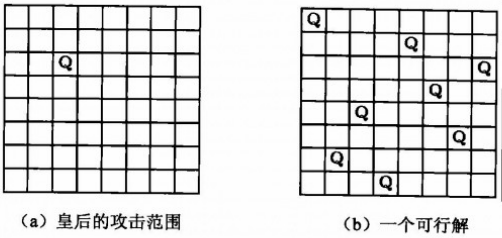
\includegraphics[width=240pt]{eight-queen.png} \\
\figcaption{八皇后问题}\label{fig:eightQueens}
\end{center}

\subsubsection{分析}
最简单的暴力枚举方法是,从64个格子中选一个子集,使得子集含有8个格子,且任意两个格子
都不在同一行、同一列或同一个对角线上。这正是子集枚举问题,然而64个格子的子集有$2^{64}$个,
太大了,这并不是一个很好的模型。

第二个思路是,从64个格子中选8个格子,这是组合生成问题。根据组合数学,有 $C_{64}^{8} \approx 4.426 \times 10^9$ 种方案,
比第一种方案优秀,但仍然不够好。

经过思考不难发现,由于每一行只能放一个皇后,那么第一行有8种选择,第二行有7中选择,…,
第8行有1中选择,总共有$8!=40320$个方案。如果用C[x]表示第x行皇后的列编号,则问题变成了一个
全排列生成问题,枚举量不会超过8!。

\subsubsection{代码}
\begin{Codex}[label=eight_queen.c]
#include <stdio.h>
#include <stdlib.h>

#define N 8 // 皇后的个数,也是棋盘的长和宽

int total = 0;  // 可行解的总数
int C[N];  // C[i]表示第i行皇后所在的列编号

/**
 * @brief 输出所有可行的棋局,按列打印.
 *
 * http://poj.grids.cn/practice/2698/ , 这题需要按列打印
 *
 * @return 无
 */
void output() {
    int i, j;
    printf("No. %d\n", total);
    for (j = 0; j < N; ++j) {
        for (i = 0; i < N; ++i) {
            if (C[i] != j) {
                printf("0 ");
            } else {
                printf("1 ");
            }
        }
        printf("\n");
    }
}

/**
 * @brief 输出所有可行的棋局,按行打印.
 * @return 无
 */
void output1() {
    int i, j;
    printf("No. %d\n", total);
    for (i = 0; i < N; ++i) {
        for (j = 0; j < N; ++j) {
            if (j != C[i]) {
                printf("0 ");
            } else {
                printf("1 ");
            }
        }
        printf("\n");
    }
}

/**
 * @brief 检查当前位置(row, column)能否放置皇后.
 *
 * @param[in] row 当前行
 * @return 能则返回1,不能则返回0
 */
int check(const int row, const int column) {
    int ok = 1;
    int i;
    for(i = 0; i < row; ++i) {
        // 两个点的坐标为(row, column), (i, C[i])
        // 检查是否在同一列,或对角线上
        if(column == C[i] || row - i == column - C[i] ||
            row - i == C[i] - column) {
            ok = 0;
            break;
        }
    }
    return ok;
}

/**
 * @brief 八皇后,深搜
 *
 * @param[in] row 搜索当前行,该在哪一列上放一个皇后
 * @return 可行解的个数
 */
int search(const int row) {
    int j;
    if (row == N) { // 终止条件,也是收敛条件,意味着找到了一个可行解
        ++total;
        output();
        return total;
    }

    for (j = 0; j < N; ++j) {  // 一列一列的试
        const int ok = check(row, j);
        if (ok) {  // 如果合法,继续递归
            C[row] = j;
            search(row + 1);
        }
    }

    return total;
}

// 表示已经放置的皇后占据了哪些列
int columns[N];
// 占据了哪些主对角线
int principal_diagonals[2 * N];
// 占据了哪些副对角线
int counter_diagonals[2 * N];

/**
 * @brief 检查当前位置(row, column)能否放置皇后.
 *
 * @param[in] row, 当前行
 * @return 能则返回1,不能则返回0
 */
int check2(const int row, const int column) {
    return columns[column] == 0 && principal_diagonals[row + column] == 0
        && counter_diagonals[row - column + N] == 0;
}

/**
 * @brief 八皇后,深搜,更优化的版本,用空间换时间
 *
 * @param[in] row 搜索当前行,该在哪一列上放一个皇后
 * @return 可行解的个数
 */
int search2(const int row) {
    int j;
    if (row == N) { // 终止条件,也是收敛条件,意味着找到了一个可行解
        ++total;
        output();
        return total;
    }

    for (j = 0; j < N; ++j) {  // 一列一列的试
        const int ok = check2(row, j);
        if (ok) {  // 如果合法,继续递归
            // 执行扩展动作
            C[row] = j;
            columns[j] = principal_diagonals[row + j] =
                    counter_diagonals[row - j + N] = 1;
            search2(row + 1);
            // 撤销动作
            C[row] = -1;  // 这句可以省略,因为C[row]会被覆盖掉
            columns[j] = principal_diagonals[row + j] =
                    counter_diagonals[row - j + N] = 0;
        }
    }

    return total;
}

int main() {
    // search(0);
    search2(0);
    return 0;
}
\end{Codex}

\subsubsection{相关的题目}
与本题相同的题目:
\begindot
\item 《算法竞赛入门经典》\footnote{刘汝佳,算法竞赛入门经典,清华大学出版社,2009} 第123页7.4.1节
\item 百练 2698 八皇后问题, \myurl{http://poj.grids.cn/practice/2698/}
\item wikioi 1295 N皇后问题, \myurl{http://www.wikioi.com/problem/1295/}
\myenddot

与本题相似的题目:
\begindot
\item POJ 1321 棋盘问题, \myurl{http://poj.org/problem?id=1321}
\myenddot


\section{还原IP地址} %%%%%%%%%%%%%%%%%%%%%%%%%%%%%%

\subsubsection{描述}
本题是 LeetCode Online Judge上的"Restore IP Addresses"。

给定一个只包含数字的字符串,还原出所有合法的IP地址。

例如:给定"25525511135",返回["255.255.11.135", "255.255.111.35"]。 (顺序无关紧要)

\subsubsection{分析}
这题很明显分为四步,有层次,因此可以尝试用回溯法解决。

\subsubsection{代码}
\begin{Codex}[label=restore_ip_adresses.cpp]
// LeetCode, Restore IP Addresses
class Solution {
public:
    vector<string> restoreIpAddresses(string s) {
        vector<string> result;
        string ip; // 存放中间结果
        dfs(s, 0, 0, ip, result);
        return result;
    }

    /**
     * @brief 解析字符串
     * @param[in] s 字符串,输入数据
     * @param[in] startIndex 从s的哪里开始
     * @param[in] step 当前步骤编号,从0开始编号,取值为0,1,2,3,4表示结束了
     * @param[out] intermediate 当前解析出来的中间结果
     * @param[out] result 存放所有可能的IP地址
     * @return 无
     */
    void dfs(string s, int start, int step, string ip,
            vector<string> &result) {
        if (s.size() - start > (4 - step) * 3)
            return;  // 非法结果,剪枝
        if (s.size() - start < (4 - step))
            return;  // 非法结果,剪枝

        if (start == s.size() && step == 4) {  // 找到一个合法解
            ip.resize(ip.size() - 1);
            result.push_back(ip);
            return;
        }

        int num = 0;
        for (int i = start; i < start + 3; i++) {
            num = num * 10 + (s[i] - '0');

            if (num <= 255) {  // 当前结点合法,则继续往下递归
                ip += s[i];
                dfs(s, i + 1, step + 1, ip + '.', result);
            }
            if (num == 0) break;  // 不允许前缀0,但允许单个0
        }
    }
};
\end{Codex}


\section{Combination Sum} %%%%%%%%%%%%%%%%%%%%%%%%%%%%%%

\subsubsection{描述}
本题是 LeetCode Online Judge上的"Combination Sum"。

给定一个数的集合(C)和一个目标数(T),找到C中所有不重复的组合,让这些被选出来的数加起来等于T。

每一个数可以被选无数次。

注意:
\begindot
\item 所有的数(包括目标)都是正整数
\item 一个组合($a_1,a_2,\cdot,a_k$)中的元素必须以非递减顺序排列
\item 一个组合不能与另一个组合重复
\myenddot

例如,给定一组数2,3,6,7,和目标7,则答案是
\begin{Code}
[7]
[2, 2, 3] 
\end{Code}

\subsubsection{分析}
这题没有固定的步骤数,但是步骤也是有限的,因此可以尝试用回溯法。

\subsubsection{代码}

\begin{Codex}[label=combination_sum.cpp]
// LeetCode, Combination Sum
class Solution {
public:
    vector<vector<int> > combinationSum(vector<int> &nums, int target) {
        sort(nums.begin(), nums.end());
        vector<vector<int> > result; // 最终结果
        vector<int> intermediate; // 中间结果
        dfs(nums, target, 0, intermediate, result);
        return result;
    }

private:
    void dfs(vector<int>& nums, int gap, int level, vector<int>& intermediate,
            vector<vector<int> > &result) {
        if (gap == 0) {  // 找到一个合法解
            result.push_back(intermediate);
            return;
        }
        for (size_t i = level; i < nums.size(); i++) { // 扩展状态
            if (gap < nums[i]) return; // 剪枝

            intermediate.push_back(nums[i]); // 执行扩展动作
            dfs(nums, gap - nums[i], i, intermediate, result);
            intermediate.pop_back();  // 撤销动作
        }
    }
};
\end{Codex}


\section{Combination Sum II} %%%%%%%%%%%%%%%%%%%%%%%%%%%%%%

\subsubsection{描述}
本题是 LeetCode Online Judge上的"Combination Sum II"。

本题与上一题唯一不同的是,每个数只能使用一次。

\subsubsection{分析}
这题没有固定的步骤数,但是步骤也是有限的,因此可以尝试用回溯法。

\subsubsection{代码}
\begin{Codex}[label=combination_sum2.cpp]
// LeetCode, Combination Sum II
class Solution {
public:
    vector<vector<int> > combinationSum2(vector<int> &nums, int target) {
        sort(nums.begin(), nums.end()); // 跟第 50 行配合,
                                             // 确保每个元素最多只用一次
        vector<vector<int> > result;
        vector<int> intermediate;
        dfs(nums, target, 0, intermediate, result);
        return result;
    }
private:
    // 使用nums[index, nums.size())之间的元素,能找到的所有可行解
    static void dfs(vector<int> &nums, int gap, int index,
            vector<int> &intermediate, vector<vector<int> > &result) {
        if (gap == 0) {  //  找到一个合法解
            result.push_back(intermediate);
            return;
        }

        int previous = -1;
        for (size_t i = index; i < nums.size(); i++) {
            // 如果上一轮循环没有选nums[i],则本次循环就不能再选nums[i],
            // 确保nums[i]最多只用一次
            if (previous == nums[i]) continue;

            if (gap < nums[i]) return;  // 剪枝

            previous = nums[i];

            intermediate.push_back(nums[i]);
            dfs(nums, gap - nums[i], i + 1, intermediate, result);
            intermediate.pop_back();  // 恢复环境
        }
    }
};
\end{Codex}



\section{Palindrome Partitioning} %%%%%%%%%%%%%%%%%%%%%%%%%%%%%%
\label{sec:palindrome-partitioning}


\subsubsection{描述}
Given a string s, partition s such that every substring of the partition is a palindrome.

Return all possible palindrome partitioning of s.

For example, given \code{s = "aab"},
Return
\begin{Code}
	[
	["aa","b"],
	["a","a","b"]
	]
\end{Code}


\subsubsection{分析}
在每一步都可以判断中间结果是否为合法结果,用回溯法。

一个长度为n的字符串,有$n-1$个地方可以砍断,每个地方可断可不断,因此复杂度为$O(2^{n-1})$


\subsubsection{深搜1}
\begin{Code}
	//LeetCode, Palindrome Partitioning
	// 时间复杂度O(2^n),空间复杂度O(n)
	class Solution {
		public:
		vector<vector<string>> partition(string s) {
			vector<vector<string>> result;
			vector<string> path;  // 一个partition方案
			dfs(s, path, result, 0, 1);
			return result;
		}
		
		// s[0, prev-1]之间已经处理,保证是回文串
		// prev 表示s[prev-1]与s[prev]之间的空隙位置,start同理
		void dfs(string &s, vector<string>& path,
		vector<vector<string>> &result, size_t prev, size_t start) {
			if (start == s.size()) { // 最后一个隔板
				if (isPalindrome(s, prev, start - 1)) { // 必须使用
					path.push_back(s.substr(prev, start - prev));
					result.push_back(path);
					path.pop_back();
				}
				return;
			}
			// 不断开
			dfs(s, path, result, prev, start + 1);
			// 如果[prev, start-1] 是回文,则可以断开,也可以不断开(上一行已经做了)
			if (isPalindrome(s, prev, start - 1)) {
				// 断开
				path.push_back(s.substr(prev, start - prev));
				dfs(s, path, result, start, start + 1);
				path.pop_back();
			}
		}
		
		bool isPalindrome(const string &s, int start, int end) {
			while (start < end && s[start] == s[end]) {
				++start;
				--end;
			}
			return start >= end;
		}
	};
\end{Code}

\subsubsection{深搜2}
另一种写法,更加简洁。这种写法也在 Combination Sum, Combination Sum II 中出现过。
\begin{Code}
	//LeetCode, Palindrome Partitioning
	// 时间复杂度O(2^n),空间复杂度O(n)
	class Solution {
		public:
		vector<vector<string>> partition(string s) {
			vector<vector<string>> result;
			vector<string> path;  // 一个partition方案
			DFS(s, path, result, 0);
			return result;
		}
		// 搜索必须以s[start]开头的partition方案
		void DFS(string &s, vector<string>& path,
		vector<vector<string>> &result, int start) {
			if (start == s.size()) {
				result.push_back(path);
				return;
			}
			for (int i = start; i < s.size(); i++) {
				if (isPalindrome(s, start, i)) { // 从i位置砍一刀
					path.push_back(s.substr(start, i - start + 1));
					DFS(s, path, result, i + 1);  // 继续往下砍
					path.pop_back(); // 撤销上上行
				}
			}
		}
		bool isPalindrome(const string &s, int start, int end) {
			while (start < end && s[start] == s[end]) {
				++start;
				--end;
			}
			return start >= end;
		}
	};
\end{Code}


\subsubsection{动规}
\begin{Code}
	// LeetCode, Palindrome Partitioning
	// 动规,时间复杂度O(n^2),空间复杂度O(1)
	class Solution {
		public:
		vector<vector<string> > partition(string s) {
			const int n = s.size();
			bool p[n][n]; // whether s[i,j] is palindrome
			fill_n(&p[0][0], n * n, false);
			for (int i = n - 1; i >= 0; --i)
			for (int j = i; j < n; ++j)
			p[i][j] = s[i] == s[j] && ((j - i < 2) || p[i + 1][j - 1]);
			
			vector<vector<string> > sub_palins[n]; // sub palindromes of s[0,i]
			for (int i = n - 1; i >= 0; --i) {
				for (int j = i; j < n; ++j)
				if (p[i][j]) {
					const string palindrome = s.substr(i, j - i + 1);
					if (j + 1 < n) {
						for (auto v : sub_palins[j + 1]) {
							v.insert(v.begin(), palindrome);
							sub_palins[i].push_back(v);
						}
					} else {
					sub_palins[i].push_back(vector<string> { palindrome });
				}
			}
		}
		return sub_palins[0];
	}
};
\end{Code}


\subsubsection{相关题目}

\begindot
\item Palindrome Partitioning II,见 \S \ref{sec:palindrome-partitioning-ii}
\myenddot


\section{Unique Paths} %%%%%%%%%%%%%%%%%%%%%%%%%%%%%%
\label{sec:unique-paths}


\subsubsection{描述}
A robot is located at the top-left corner of a $m \times n$ grid (marked 'Start' in the diagram below).

The robot can only move either down or right at any point in time. The robot is trying to reach the bottom-right corner of the grid (marked 'Finish' in the diagram below).

How many possible unique paths are there?

\begin{center}
	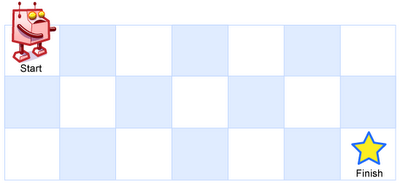
\includegraphics[width=200pt]{robot-maze.png}\\
	\figcaption{Above is a $3 \times 7$ grid. How many possible unique paths are there?}\label{fig:unique-paths}
\end{center}

\textbf{Note}: $m$ and $n$ will be at most 100.


\subsection{深搜}
深搜,小集合可以过,大集合会超时

\subsubsection{代码}
\begin{Code}
	// LeetCode, Unique Paths
	// 深搜,小集合可以过,大集合会超时
	// 时间复杂度O(n^4),空间复杂度O(n)
	class Solution {
		public:
		int uniquePaths(int m, int n) {
			if (m < 1 || n < 1) return 0; // 终止条件
			
			if (m == 1 && n == 1) return 1; // 收敛条件
			
			return uniquePaths(m - 1, n) + uniquePaths(m, n - 1);
		}
	};
\end{Code}


\subsection{备忘录法}
给前面的深搜,加个缓存,就可以过大集合了。即备忘录法。

\subsubsection{代码}
\begin{Code}
	// LeetCode, Unique Paths
	// 深搜 + 缓存,即备忘录法
	// 时间复杂度O(n^2),空间复杂度O(n^2)
	class Solution {
		public:
		int uniquePaths(int m, int n) {
			// 0行和0列未使用
			this->f = vector<vector<int> >(m + 1, vector<int>(n + 1, 0));
			return dfs(m, n);
		}
		private:
		vector<vector<int> > f;  // 缓存
		
		int dfs(int x, int y) {
			if (x < 1 || y < 1) return 0; // 数据非法,终止条件
			
			if (x == 1 && y == 1) return 1; // 回到起点,收敛条件
			
			return getOrUpdate(x - 1, y) + getOrUpdate(x, y - 1);
		}
		
		int getOrUpdate(int x, int y) {
			if (f[x][y] > 0) return f[x][y];
			else return f[x][y] = dfs(x, y);
		}
	};
\end{Code}


\subsection{动规}
既然可以用备忘录法自顶向下解决,也一定可以用动规自底向上解决。

设状态为\fn{f[i][j]},表示从起点$(1,1)$到达$(i,j)$的路线条数,则状态转移方程为:
\begin{Code}
	f[i][j]=f[i-1][j]+f[i][j-1]
\end{Code}


\subsubsection{代码}
\begin{Code}
	// LeetCode, Unique Paths
	// 动规,滚动数组
	// 时间复杂度O(n^2),空间复杂度O(n)
	class Solution {
		public:
		int uniquePaths(int m, int n) {
			vector<int> f(n, 0);
			f[0] = 1;
			for (int i = 0; i < m; i++) {
				for (int j = 1; j < n; j++) {
					// 左边的f[j],表示更新后的f[j],与公式中的f[i[[j]对应
					// 右边的f[j],表示老的f[j],与公式中的f[i-1][j]对应
					f[j] = f[j - 1] + f[j];
				}
			}
			return f[n - 1];
		}
	};
\end{Code}


\subsection{数学公式}
一个$m$行,$n$列的矩阵,机器人从左上走到右下总共需要的步数是$m+n-2$,其中向下走的步数是$m-1$,因此问题变成了在$m+n-2$个操作中,选择$m–1$个时间点向下走,选择方式有多少种。即 $C_{m+n-2}^{m-1}$ 。

\subsubsection{代码}
\begin{Code}
	// LeetCode, Unique Paths
	// 数学公式
	class Solution {
		public:
		typedef long long int64_t;
		// 求阶乘, n!/(start-1)!,即 n*(n-1)...start,要求 n >= 1
		static int64_t factor(int n, int start = 1) {
			int64_t  ret = 1;
			for(int i = start; i <= n; ++i)
			ret *= i;
			return ret;
		}
		// 求组合数 C_n^k
		static int64_t combination(int n, int k) {
			// 常数优化
			if (k == 0) return 1;
			if (k == 1) return n;
			
			int64_t ret = factor(n, k+1);
			ret /= factor(n - k);
			return ret;
		}
		
		int uniquePaths(int m, int n) {
			// max 可以防止n和k差距过大,从而防止combination()溢出
			return combination(m+n-2, max(m-1, n-1));
		}
	};
\end{Code}


\subsubsection{相关题目}
\begindot
\item Unique Paths II,见 \S \ref{sec:unique-paths-ii}
\item Minimum Path Sum, 见 \S \ref{sec:minimum-path-sum}
\myenddot


\section{Unique Paths II} %%%%%%%%%%%%%%%%%%%%%%%%%%%%%%
\label{sec:unique-paths-ii}


\subsubsection{描述}
Follow up for "Unique Paths":

Now consider if some obstacles are added to the grids. How many unique paths would there be?

An obstacle and empty space is marked as 1 and 0 respectively in the grid.

For example,

There is one obstacle in the middle of a $3 \times 3$ grid as illustrated below.
\begin{Code}
	[
	[0,0,0],
	[0,1,0],
	[0,0,0]
	]
\end{Code}

The total number of unique paths is 2.

Note: $m$ and $n$ will be at most 100.


\subsection{备忘录法}
在上一题的基础上改一下即可。相比动规,简单得多。

\subsubsection{代码}
\begin{Code}
	// LeetCode, Unique Paths II
	// 深搜 + 缓存,即备忘录法
	class Solution {
		public:
		int uniquePathsWithObstacles(vector<vector<int> > &obstacleGrid) {
			const int m = obstacleGrid.size();
			const int n = obstacleGrid[0].size();
			// 0行和0列未使用
			this->f = vector<vector<int> >(m + 1, vector<int>(n + 1, 0));
			return dfs(obstacleGrid, m, n);
		}
		private:
		vector<vector<int> > f;  // 缓存
		
		int dfs(const vector<vector<int> > &obstacleGrid,
		int x, int y) {
			if (x < 1 || y < 1) return 0; // 数据非法,终止条件
			
			// (x,y)是障碍
			if (obstacleGrid[x-1][y-1]) return 0;
			
			if (x == 1 and y == 1) return 1; // 回到起点,收敛条件
			
			return getOrUpdate(obstacleGrid, x - 1, y) +
			getOrUpdate(obstacleGrid, x, y - 1);
		}
		
		int getOrUpdate(const vector<vector<int> > &obstacleGrid,
		int x, int y) {
			if (f[x][y] > 0) return f[x][y];
			else return f[x][y] = dfs(obstacleGrid, x, y);
		}
	};
\end{Code}


\subsection{动规}
与上一题类似,但要特别注意第一列的障碍。在上一题中,第一列全部是1,但是在这一题中不同,第一列如果某一行有障碍物,那么后面的行应该为0。


\subsubsection{代码}
\begin{Code}
	// LeetCode, Unique Paths II
	// 动规,滚动数组
	// 时间复杂度O(n^2),空间复杂度O(n)
	class Solution {
		public:
		int uniquePathsWithObstacles(vector<vector<int> > &obstacleGrid) {
			const int m = obstacleGrid.size();
			const int n = obstacleGrid[0].size();
			if (obstacleGrid[0][0] || obstacleGrid[m-1][n-1]) return 0;
			
			vector<int> f(n, 0);
			f[0] = obstacleGrid[0][0] ? 0 : 1;
			
			for (int i = 0; i < m; i++)
			for (int j = 0; j < n; j++)
			f[j] = obstacleGrid[i][j] ? 0 : (j == 0 ? 0 : f[j - 1]) + f[j];
			
			return f[n - 1];
		}
	};
\end{Code}


\subsubsection{相关题目}
\begindot
\item Unique Paths,见 \S \ref{sec:unique-paths}
\item Minimum Path Sum, 见 \S \ref{sec:minimum-path-sum}
\myenddot


\section{N-Queens} %%%%%%%%%%%%%%%%%%%%%%%%%%%%%%
\label{sec:n-queens}


\subsubsection{描述}
The \emph{n-queens puzzle} is the problem of placing n queens on an $n \times n$ chessboard such that no two queens attack each other.

\begin{center}
	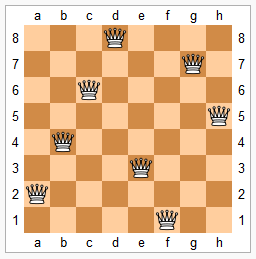
\includegraphics{8-queens.png}\\
	\figcaption{Eight Queens}\label{fig:8-queens}
\end{center}

Given an integer $n$, return all distinct solutions to the n-queens puzzle.

Each solution contains a distinct board configuration of the n-queens' placement, where \fn{'Q'} and \fn{'.'} both indicate a queen and an empty space respectively.

For example,
There exist two distinct solutions to the 4-queens puzzle:
\begin{Code}
	[
	[".Q..",  // Solution 1
	"...Q",
	"Q...",
	"..Q."],
	
	["..Q.",  // Solution 2
	"Q...",
	"...Q",
	".Q.."]
	]
\end{Code}


\subsubsection{分析}
经典的深搜题。

\subsubsection{代码}
\begin{Code}
	// LeetCode, N-Queens
	// 深搜+剪枝
	// 时间复杂度O(n!),空间复杂度O(n)
	class Solution {
		public:
		vector<vector<string> > solveNQueens(int n) {
			this->columns = vector<int>(n, 0);
			this->main_diag = vector<int>(2 * n, 0);
			this->anti_diag = vector<int>(2 * n, 0);
			
			vector<vector<string> > result;
			vector<int> C(n, 0);  // C[i]表示第i行皇后所在的列编号
			dfs(C, result, 0);
			return result;
		}
		private:
		// 这三个变量用于剪枝
		vector<int> columns;  // 表示已经放置的皇后占据了哪些列
		vector<int> main_diag;  // 占据了哪些主对角线
		vector<int> anti_diag;  // 占据了哪些副对角线
		
		void dfs(vector<int> &C, vector<vector<string> > &result, int row) {
			const int N = C.size();
			if (row == N) { // 终止条件,也是收敛条件,意味着找到了一个可行解
				vector<string> solution;
				for (int i = 0; i < N; ++i) {
					string s(N, '.');
					for (int j = 0; j < N; ++j) {
						if (j == C[i]) s[j] = 'Q';
					}
					solution.push_back(s);
				}
				result.push_back(solution);
				return;
			}
			
			for (int j = 0; j < N; ++j) {  // 扩展状态,一列一列的试
				const bool ok = columns[j] == 0 && main_diag[row + j] == 0 &&
				anti_diag[row - j + N] == 0;
				if (!ok) continue;  // 剪枝:如果合法,继续递归
				// 执行扩展动作
				C[row] = j;
				columns[j] = main_diag[row + j] = anti_diag[row - j + N] = 1;
				dfs(C, result, row + 1);
				// 撤销动作
				// C[row] = 0;
				columns[j] = main_diag[row + j] = anti_diag[row - j + N] = 0;
			}
		}
	};
\end{Code}


\subsubsection{相关题目}
\begindot
\item N-Queens II,见 \S \ref{sec:n-queens-ii}
\myenddot


\section{N-Queens II} %%%%%%%%%%%%%%%%%%%%%%%%%%%%%%
\label{sec:n-queens-ii}


\subsubsection{描述}
Follow up for N-Queens problem.

Now, instead outputting board configurations, return the total number of distinct solutions.


\subsubsection{分析}
只需要输出解的个数,不需要输出所有解,代码要比上一题简化很多。设一个全局计数器,每找到一个解就增1。


\subsubsection{代码}
\begin{Code}
	// LeetCode, N-Queens II
	// 深搜+剪枝
	// 时间复杂度O(n!),空间复杂度O(n)
	class Solution {
		public:
		int totalNQueens(int n) {
			this->count = 0;
			this->columns = vector<int>(n, 0);
			this->main_diag = vector<int>(2 * n, 0);
			this->anti_diag = vector<int>(2 * n, 0);
			
			vector<int> C(n, 0);  // C[i]表示第i行皇后所在的列编号
			dfs(C, 0);
			return this->count;
		}
		private:
		int count; // 解的个数
		// 这三个变量用于剪枝
		vector<int> columns;  // 表示已经放置的皇后占据了哪些列
		vector<int> main_diag;  // 占据了哪些主对角线
		vector<int> anti_diag;  // 占据了哪些副对角线
		
		void dfs(vector<int> &C, int row) {
			const int N = C.size();
			if (row == N) { // 终止条件,也是收敛条件,意味着找到了一个可行解
				++this->count;
				return;
			}
			
			for (int j = 0; j < N; ++j) {  // 扩展状态,一列一列的试
				const bool ok = columns[j] == 0 &&
				main_diag[row + j] == 0 &&
				anti_diag[row - j + N] == 0;
				if (!ok) continue;  // 剪枝:如果合法,继续递归
				// 执行扩展动作
				C[row] = j;
				columns[j] = main_diag[row + j] =
				anti_diag[row - j + N] = 1;
				dfs(C, row + 1);
				// 撤销动作
				// C[row] = 0;
				columns[j] = main_diag[row + j] =
				anti_diag[row - j + N] = 0;
			}
		}
	};
\end{Code}


\subsubsection{相关题目}
\begindot
\item N-Queens,见 \S \ref{sec:n-queens}
\myenddot


\section{Restore IP Addresses} %%%%%%%%%%%%%%%%%%%%%%%%%%%%%%
\label{sec:restore-ip-addresses}


\subsubsection{描述}
Given a string containing only digits, restore it by returning all possible valid IP address combinations.

For example:
Given \code{"25525511135"},

return \code{["255.255.11.135", "255.255.111.35"]}. (Order does not matter)


\subsubsection{分析}
必须要走到底部才能判断解是否合法,深搜。


\subsubsection{代码}
\begin{Code}
	// LeetCode, Restore IP Addresses
	// 时间复杂度O(n^4),空间复杂度O(n)
	class Solution {
		public:
		vector<string> restoreIpAddresses(string s) {
			vector<string> result;
			string ip; // 存放中间结果
			dfs(s, 0, 0, ip, result);
			return result;
		}
		
		/**
		* @brief 解析字符串
		* @param[in] s 字符串,输入数据
		* @param[in] startIndex 从s的哪里开始
		* @param[in] step 当前步骤编号,从0开始编号,取值为0,1,2,3,4表示结束了
		* @param[out] intermediate 当前解析出来的中间结果
		* @param[out] result 存放所有可能的IP地址
		* @return 无
		*/
		void dfs(string s, size_t start, size_t step, string ip,
		vector<string> &result) {
			if (start == s.size() && step == 4) {  // 找到一个合法解
				ip.resize(ip.size() - 1);
				result.push_back(ip);
				return;
			}
			
			if (s.size() - start > (4 - step) * 3)
			return;  // 剪枝
			if (s.size() - start < (4 - step))
			return;  // 剪枝
			
			int num = 0;
			for (size_t i = start; i < start + 3; i++) {
				num = num * 10 + (s[i] - '0');
				
				if (num <= 255) {  // 当前结点合法,则继续往下递归
					ip += s[i];
					dfs(s, i + 1, step + 1, ip + '.', result);
				}
				if (num == 0) break;  // 不允许前缀0,但允许单个0
			}
		}
	};
\end{Code}


\subsubsection{相关题目}
\begindot
\item 无
\myenddot


\section{Combination Sum} %%%%%%%%%%%%%%%%%%%%%%%%%%%%%%
\label{sec:combination-sum}


\subsubsection{描述}
Given a set of candidate numbers ($C$) and a target number ($T$), find all unique combinations in $C$ where the candidate numbers sums to $T$.

The same repeated number may be chosen from $C$ \emph{unlimited} number of times.

Note:
\begindot
\item All numbers (including target) will be positive integers.
\item Elements in a combination ($a_1, a_2, ..., a_k$) must be in non-descending order. (ie, $a_1 \leq a_2 \leq ... \leq a_k$).
\item The solution set must not contain duplicate combinations.
\myenddot

For example, given candidate set \fn{2,3,6,7} and target \fn{7}, 
A solution set is: 
\begin{Code}
	[7] 
	[2, 2, 3] 
\end{Code}


\subsubsection{分析}
无


\subsubsection{代码}
\begin{Code}
	// LeetCode, Combination Sum
	// 时间复杂度O(n!),空间复杂度O(n)
	class Solution {
		public:
		vector<vector<int> > combinationSum(vector<int> &nums, int target) {
			sort(nums.begin(), nums.end());
			vector<vector<int> > result; // 最终结果
			vector<int> intermediate; // 中间结果
			dfs(nums, target, 0, intermediate, result);
			return result;
		}
		
		private:
		void dfs(vector<int>& nums, int gap, int start, vector<int>& intermediate,
		vector<vector<int> > &result) {
			if (gap == 0) {  // 找到一个合法解
				result.push_back(intermediate);
				return;
			}
			for (size_t i = start; i < nums.size(); i++) { // 扩展状态
				if (gap < nums[i]) return; // 剪枝
				
				intermediate.push_back(nums[i]); // 执行扩展动作
				dfs(nums, gap - nums[i], i, intermediate, result);
				intermediate.pop_back();  // 撤销动作
			}
		}
	};
\end{Code}


\subsubsection{相关题目}
\begindot
\item Combination Sum II ,见 \S \ref{sec:combination-sum-ii}
\myenddot


\section{Combination Sum II} %%%%%%%%%%%%%%%%%%%%%%%%%%%%%%
\label{sec:combination-sum-ii}


\subsubsection{描述}
Given a set of candidate numbers ($C$) and a target number ($T$), find all unique combinations in $C$ where the candidate numbers sums to $T$.

The same repeated number may be chosen from $C$ \emph{once} number of times.

Note:
\begindot
\item All numbers (including target) will be positive integers.
\item Elements in a combination ($a_1, a_2, ..., a_k$) must be in non-descending order. (ie, $a_1 > a_2 > ... > a_k$).
\item The solution set must not contain duplicate combinations.
\myenddot

For example, given candidate set \fn{10,1,2,7,6,1,5} and target \fn{8}, 
A solution set is: 
\begin{Code}
	[1, 7] 
	[1, 2, 5] 
	[2, 6] 
	[1, 1, 6]
\end{Code}


\subsubsection{分析}
无


\subsubsection{代码}
\begin{Code}
	// LeetCode, Combination Sum II
	// 时间复杂度O(n!),空间复杂度O(n)
	class Solution {
		public:
		vector<vector<int> > combinationSum2(vector<int> &nums, int target) {
			sort(nums.begin(), nums.end()); // 跟第 50 行配合,
			// 确保每个元素最多只用一次
			vector<vector<int> > result;
			vector<int> intermediate;
			dfs(nums, target, 0, intermediate, result);
			return result;
		}
		private:
		// 使用nums[start, nums.size())之间的元素,能找到的所有可行解
		static void dfs(vector<int> &nums, int gap, int start,
		vector<int> &intermediate, vector<vector<int> > &result) {
			if (gap == 0) {  //  找到一个合法解
				result.push_back(intermediate);
				return;
			}
			
			int previous = -1;
			for (size_t i = start; i < nums.size(); i++) {
				// 如果上一轮循环没有选nums[i],则本次循环就不能再选nums[i],
				// 确保nums[i]最多只用一次
				if (previous == nums[i]) continue;
				
				if (gap < nums[i]) return;  // 剪枝
				
				previous = nums[i];
				
				intermediate.push_back(nums[i]);
				dfs(nums, gap - nums[i], i + 1, intermediate, result);
				intermediate.pop_back();  // 恢复环境
			}
		}
	};
\end{Code}


\subsubsection{相关题目}
\begindot
\item Combination Sum ,见 \S \ref{sec:combination-sum}
\myenddot


\section{Generate Parentheses } %%%%%%%%%%%%%%%%%%%%%%%%%%%%%%
\label{sec:generate-parentheses}


\subsubsection{描述}
Given $n$ pairs of parentheses, write a function to generate all combinations of well-formed parentheses.

For example, given $n = 3$, a solution set is:
\begin{Code}
	"((()))", "(()())", "(())()", "()(())", "()()()"
\end{Code}

\subsubsection{分析}
小括号串是一个递归结构,跟单链表、二叉树等递归结构一样,首先想到用递归。

一步步构造字符串。当左括号出现次数$<n$时,就可以放置新的左括号。当右括号出现次数小于左括号出现次数时,就可以放置新的右括号。


\subsubsection{代码1}
\begin{Code}
	// LeetCode, Generate Parentheses
	// 时间复杂度O(TODO),空间复杂度O(n)
	class Solution {
		public:
		vector<string> generateParenthesis(int n) {
			vector<string> result;
			if (n > 0) generate(n, "", 0, 0, result);
			return result;
		}
		// l 表示 ( 出现的次数, r 表示 ) 出现的次数
		void generate(int n, string s, int l, int r, vector<string> &result) {
			if (l == n) {
				result.push_back(s.append(n - r, ')'));
				return;
			}
			generate(n, s + '(', l + 1, r, result);
			if (l > r) generate(n, s + ")", l, r + 1, result);
		}
	};
\end{Code}


\subsubsection{代码2}
另一种递归写法,更加简洁。
\begin{Code}
	// LeetCode, Generate Parentheses
	// @author 连城 (http://weibo.com/lianchengzju)
	class Solution {
		public:
		vector<string> generateParenthesis (int n) {
			if (n == 0) return vector<string>(1, "");
			if (n == 1) return vector<string> (1, "()");
			vector<string> result;
			
			for (int i = 0; i < n; ++i)
			for (auto inner : generateParenthesis (i))
			for (auto outer : generateParenthesis (n - 1 - i))
			result.push_back ("(" + inner + ")" + outer);
			
			return result;
		}
	};
\end{Code}


\subsubsection{相关题目}
\begindot
\item Valid Parentheses, 见 \S \ref{sec:valid-parentheses}
\item Longest Valid Parentheses, 见 \S \ref{sec:longest-valid-parentheses}
\myenddot


\section{Sudoku Solver} %%%%%%%%%%%%%%%%%%%%%%%%%%%%%%
\label{sec:sudoku-solver}


\subsubsection{描述}
Write a program to solve a Sudoku puzzle by filling the empty cells.

Empty cells are indicated by the character \fn{'.'}.

You may assume that there will be only one unique solution.

\begin{center}
	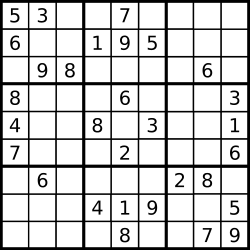
\includegraphics[width=150pt]{sudoku.png}\\
	\figcaption{A sudoku puzzle...}\label{fig:sudoku}
\end{center}

\begin{center}
	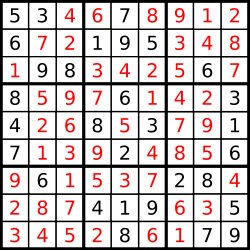
\includegraphics[width=150pt]{sudoku-solution.png}\\
	\figcaption{...and its solution numbers marked in red}\label{fig:sudoku-solution}
\end{center}


\subsubsection{分析}
无。


\subsubsection{代码}
\begin{Code}
	// LeetCode, Sudoku Solver
	// 时间复杂度O(9^4),空间复杂度O(1)
	class Solution {
		public:
		bool solveSudoku(vector<vector<char> > &board) {
			for (int i = 0; i < 9; ++i)
			for (int j = 0; j < 9; ++j) {
				if (board[i][j] == '.') {
					for (int k = 0; k < 9; ++k) {
						board[i][j] = '1' + k;
						if (isValid(board, i, j) && solveSudoku(board))
						return true;
						board[i][j] = '.';
					}
					return false;
				}
			}
			return true;
		}
		private:
		// 检查 (x, y) 是否合法
		bool isValid(const vector<vector<char> > &board, int x, int y) {
			int i, j;
			for (i = 0; i < 9; i++) // 检查 y 列
			if (i != x && board[i][y] == board[x][y])
			return false;
			for (j = 0; j < 9; j++) // 检查 x 行
			if (j != y && board[x][j] == board[x][y])
			return false;
			for (i = 3 * (x / 3); i < 3 * (x / 3 + 1); i++)
			for (j = 3 * (y / 3); j < 3 * (y / 3 + 1); j++)
			if ((i != x || j != y) && board[i][j] == board[x][y])
			return false;
			return true;
		}
	};
\end{Code}


\subsubsection{相关题目}
\begindot
\item Valid Sudoku, 见 \S \ref{sec:valid-sudoku}
\myenddot


\section{Word Search} %%%%%%%%%%%%%%%%%%%%%%%%%%%%%%
\label{sec:word-search}


\subsubsection{描述}
Given a 2D board and a word, find if the word exists in the grid.

The word can be constructed from letters of sequentially adjacent cell, where \fn{"adjacent"} cells are those horizontally or vertically neighbouring. The same letter cell may not 
be used more than once.

For example,
Given board =
\begin{Code}
	[
	["ABCE"],
	["SFCS"],
	["ADEE"]
	]
\end{Code}
word = \fn{"ABCCED"}, -> returns \fn{true},\\
word = \fn{"SEE"}, -> returns \fn{true},\\
word = \fn{"ABCB"}, -> returns \fn{false}.


\subsubsection{分析}
无。


\subsubsection{代码}
\begin{Code}
	// LeetCode, Word Search
	// 深搜,递归
	// 时间复杂度O(n^2*m^2),空间复杂度O(n^2)
	class Solution {
		public:
		bool exist(vector<vector<char> > &board, string word) {
			const int m = board.size();
			const int n = board[0].size();
			vector<vector<bool> > visited(m, vector<bool>(n, false));
			for (int i = 0; i < m; ++i)
			for (int j = 0; j < n; ++j)
			if (dfs(board, word, 0, i, j, visited))
			return true;
			return false;
		}
		private:
		static bool dfs(const vector<vector<char> > &board, const string &word,
		int index, int x, int y, vector<vector<bool> > &visited) {
			if (index == word.size())
			return true; // 收敛条件
			
			if (x < 0 || y < 0 || x >= board.size() || y >= board[0].size())
			return false;  // 越界,终止条件
			
			if (visited[x][y]) return false; // 已经访问过,剪枝
			
			if (board[x][y] != word[index]) return false; // 不相等,剪枝
			
			visited[x][y] = true;
			bool ret = dfs(board, word, index + 1, x - 1, y, visited) || // 上
			dfs(board, word, index + 1, x + 1, y, visited)    || // 下
			dfs(board, word, index + 1, x, y - 1, visited)    || // 左
			dfs(board, word, index + 1, x, y + 1, visited);      // 右
			visited[x][y] = false;
			return ret;
		}
	};
\end{Code}


\subsubsection{相关题目}
\begindot
\item 无
\myenddot


\section{小结} %%%%%%%%%%%%%%%%%%%%%%%%%%%%%%
\label{sec:dfs-template}


\subsection{适用场景}

\textbf{输入数据}:如果是递归数据结构,如单链表,二叉树,集合,则百分之百可以用深搜;如果是非递归数据结构,如一维数组,二维数组,字符串,图,则概率小一些。

\textbf{状态转换图}:树或者图。

\textbf{求解目标}:必须要走到最深(例如对于树,必须要走到叶子节点)才能得到一个解,这种情况适合用深搜。


\subsection{思考的步骤}
\begin{enumerate}
	\item 是求路径条数,还是路径本身(或动作序列)?深搜最常见的三个问题,求可行解的总数,求一个可行解,求所有可行解。
	\begin{enumerate}
		\item 如果是路径条数,则不需要存储路径。
		\item 
		如果是求路径本身,则要用一个数组\fn{path[]}存储路径。跟宽搜不同,宽搜虽然最终求的也是一条路径,但是需要存储扩展过程中的所有路径,在没找到答案之前所有路径都不能放弃;而深搜,在搜索过程中始终只有一条路径,因此用一个数组就足够了。
	\end{enumerate}
	
	\item 
	只要求一个解,还是要求所有解?如果只要求一个解,那找到一个就可以返回;如果要求所有解,找到了一个后,还要继续扩展,直到遍历完。广搜一般只要求一个解,因而不需要考虑这个问题(广搜当然也可以求所有解,这时需要扩展到所有叶子节点,相当于在内存中存储整个状态转换图,非常占内存,因此广搜不适合解这类问题)。
	
	\item 
	如何表示状态?即一个状态需要存储哪些些必要的数据,才能够完整提供如何扩展到下一步状态的所有信息。跟广搜不同,深搜的惯用写法,不是把数据记录在状态\fn{struct}里,而是添加函数参数(有时为了节省递归堆栈,用全局变量),\fn{struct}里的字段与函数参数一一对应。
	
	\item 
	如何扩展状态?这一步跟上一步相关。状态里记录的数据不同,扩展方法就不同。对于固定不变的数据结构(一般题目直接给出,作为输入数据),如二叉树,图等,扩展方法很简单,直接往下一层走,对于隐式图,要先在第1步里想清楚状态所带的数据,想清楚了这点,那如何扩展就很简单了。
	
	\item 关于判重
	\begin{enumerate}
		\item 是否需要判重?如果状态转换图是一棵树,则不需要判重,因为在遍历过程中不可能重复;如果状态转换图是一个DAG,则需要判重。这一点跟BFS不一样,BFS的状态转换图总是DAG,必须要判重。
		\item 怎样判重?跟广搜相同,见第 \S \ref{sec:bfs-template} 节。同时,DAG说明存在重叠子问题,此时可以用缓存加速,见第8步。
	\end{enumerate}
	
	\item 终止条件是什么?终止条件是指到了不能扩展的末端节点。对于树,是叶子节点,对于图或隐式图,是出度为0的节点。
	
	\item 
	{收敛条件是什么?收敛条件是指找到了一个合法解的时刻。如果是正向深搜(父状态处理完了才进行递归,即父状态不依赖子状态,递归语句一定是在最后,尾递归),则是指是否达到目标状态;如果是逆向深搜(处理父状态时需要先知道子状态的结果,此时递归语句不在最后),则是指是否到达初始状态。
		
		由于很多时候终止条件和收敛条件是是合二为一的,因此很多人不区分这两种条件。仔细区分这两种条件,还是很有必要的。
		
		为了判断是否到了收敛条件,要在函数接口里用一个参数记录当前的位置(或距离目标还有多远)。如果是求一个解,直接返回这个解;如果是求所有解,要在这里收集解,即把第一步中表示路径的数组\fn{path[]}复制到解集合里。}
	
	\item 如何加速?
	\begin{enumerate}
		\item 剪枝。深搜一定要好好考虑怎么剪枝,成本小收益大,加几行代码,就能大大加速。这里没有通用方法,只能具体问题具体分析,要充分观察,充分利用各种信息来剪枝,在中间节点提前返回。
		\item 缓存。
		\begin{enumerate}
			\item 
			前提条件:状态转换图是一个DAG。DAG=>存在重叠子问题=>子问题的解会被重复利用,用缓存自然会有加速效果。如果依赖关系是树状的(例如树,单链表等),没必要加缓存,因为子问题只会一层层往下,用一次就再也不会用到,加了缓存也没什么加速效果。
			\item 具体实现:可以用数组或HashMap。维度简单的,用数组;维度复杂的,用HashMap,C++有\fn{map},C++ 11以后有\fn{unordered_map},比\fn{map}快。
		\end{enumerate}
		
	\end{enumerate}
\end{enumerate}

拿到一个题目,当感觉它适合用深搜解决时,在心里面把上面8个问题默默回答一遍,代码基本上就能写出来了。对于树,不需要回答第5和第8个问题。如果读者对上面的经验总结看不懂或感觉“不实用”,很正常,因为这些经验总结是我做了很多题目后总结出来的,从思维的发展过程看,“经验总结”要晚于感性认识,所以这时候建议读者先做做前面的题目,积累一定的感性认识后,再回过头来看这一节的总结,一定会有共鸣。


\subsection{代码模板}

\begin{Codex}[label=dfs_template.cpp]
	/**
	* dfs模板.
	* @param[in] input 输入数据指针
	* @param[out] path 当前路径,也是中间结果
	* @param[out] result 存放最终结果
	* @param[inout] cur or gap 标记当前位置或距离目标的距离
	* @return 路径长度,如果是求路径本身,则不需要返回长度
	*/
	void dfs(type &input, type &path, type &result, int cur or gap) {
		if (数据非法) return 0;   // 终止条件
		if (cur == input.size()) { // 收敛条件
			// if (gap == 0) {
				将path放入result
			}
			
			if (可以剪枝) return;
			
			for(...) { // 执行所有可能的扩展动作
				执行动作,修改path
				dfs(input, step + 1 or gap--, result);
				恢复path
			}
		}
	\end{Codex}
	
	
	\subsection{深搜与回溯法的区别}
	深搜(Depth-first search, DFS)的定义见\myurl{http://en.wikipedia.org/wiki/Depth_first_search},回溯法(backtracking)的定义见\myurl{http://en.wikipedia.org/wiki/Backtracking}
	
	\textbf{回溯法 = 深搜 + 剪枝}。一般大家用深搜时,或多或少会剪枝,因此深搜与回溯法没有什么不同,可以在它们之间画上一个等号。本书同时使用深搜和回溯法两个术语,但读者可以认为二者等价。
	
	深搜一般用递归(recursion)来实现,这样比较简洁。
	
	深搜能够在候选答案生成到一半时,就进行判断,抛弃不满足要求的答案,所以深搜比暴力搜索法要快。
	
	
	\subsection{深搜与递归的区别}
	\label{sec:dfs-vs-recursion}
	
	深搜经常用递归(recursion)来实现,二者常常同时出现,导致很多人误以为他俩是一个东西。
	
	深搜,是逻辑意义上的算法,递归,是一种物理意义上的实现,它和迭代(iteration)是对应的。深搜,可以用递归来实现,也可以用栈来实现;而递归,一般总是用来实现深搜。可以说,\textbf{递归一定是深搜,深搜不一定用递归}。
	
	递归有两种加速策略,一种是\textbf{剪枝(prunning)},对中间结果进行判断,提前返回;一种是\textbf{缓存},缓存中间结果,防止重复计算,用空间换时间。
	
	其实,递归+缓存,就是 memorization。所谓\textbf{memorization}(翻译为备忘录法,见第 \S \ref{sec:dp-vs-memorization}节),就是"top-down with cache"(自顶向下+缓存),它是Donald Michie 
	在1968年创造的术语,表示一种优化技术,在top-down 形式的程序中,使用缓存来避免重复计算,从而达到加速的目的。
	
	\textbf{memorization 不一定用递归},就像深搜不一定用递归一样,可以在迭代(iterative)中使用 memorization 。\textbf{递归也不一定用 
	memorization},可以用memorization来加速,但不是必须的。只有当递归使用了缓存,它才是 memorization 。
	
	既然递归一定是深搜,为什么很多书籍都同时使用这两个术语呢?在递归味道更浓的地方,一般用递归这个术语,在深搜更浓的场景下,用深搜这个术语,读者心里要弄清楚他俩大部分时候是一回事。在单链表、二叉树等递归数据结构上,递归的味道更浓,这时用递归这个术语;在图、隐式图等数据结构上,深搜的味道更浓,这时用深搜这个术语。


\section{小结} %%%%%%%%%%%%%%%%%%%%%%%%%%%%%%
\label{sec:dfs-template}


\subsection{适用场景}

\textbf{输入数据}:如果是递归数据结构,如单链表,二叉树,集合,则百分之百可以用深搜;如果是非递归数据结构,如一维数组,二维数组,字符串,图,则概率小一些。

\textbf{状态转换图}:树或者图。

\textbf{求解目标}:必须要走到最深(例如对于树,必须要走到叶子节点)才能得到一个解,这种情况适合用深搜。


\subsection{思考的步骤}
\begin{enumerate}
\item 是求路径条数,还是路径本身(或动作序列)?深搜最常见的三个问题,求可行解的总数,求一个可行解,求所有可行解。
    \begin{enumerate}
    \item 如果是求路径本身,则要用一个数组\fn{path[]}存储路径。跟宽搜不同,宽搜虽然最终求的也是一条路径,但是需要存储扩展过程中的所有路径,在没找到答案之前所有路径都不能放弃;而深搜,在搜索过程中始终只有一条路径,因此用一个数组就足够了。
    \item 如果是路径条数,则不需要存储路径。
    \end{enumerate}

\item 只要求一个解,还是要求所有解?如果只要求一个解,那找到一个就可以返回;如果要求所有解,找到了一个后,还要继续扩展,直到遍历完。广搜一般只要求一个解,因而不需要考虑这个问题(广搜当然也可以求所有解,这时需要扩展到所有叶子节点,相当于在内存中存储整个状态转换图,非常占内存,因此广搜不适合解这类问题)。

\item 如何表示状态?即一个状态需要存储哪些些必要的数据,才能够完整提供如何扩展到下一步状态的所有信息。跟广搜不同,深搜的惯用写法,不是把数据记录在状态\fn{struct}里,而是添加函数参数(有时为了节省递归堆栈,用全局变量),\fn{struct}里的字段与函数参数一一对应。

\item 如何扩展状态?这一步跟上一步相关。状态里记录的数据不同,扩展方法就不同。对于固定不变的数据结构(一般题目直接给出,作为输入数据),如二叉树,图等,扩展方法很简单,直接往下一层走,对于隐式图,要先在第1步里想清楚状态所带的数据,想清楚了这点,那如何扩展就很简单了。

\item 关于判重
    \begin{enumerate}
    \item 如果状态转换图是一棵树,则不需要判重,因为在遍历过程中不可能重复。
    \item 如果状态转换图是一个图,则需要判重,方法跟广搜相同,见第 \S \ref{sec:bfs-template} 节。这里跟第8步中的加缓存是相同的,如果有重叠子问题,则需要判重,此时加缓存自然也是有效果的。
    \end{enumerate}

\item 终止条件是什么?终止条件是指到了不能扩展的末端节点。对于树,是叶子节点,对于图或隐式图,是出度为0的节点。

\item {收敛条件是什么?收敛条件是指找到了一个合法解的时刻。如果是正向深搜(父状态处理完了才进行递归,即父状态不依赖子状态,递归语句一定是在最后,尾递归),则是指是否达到目标状态;如果是逆向深搜(处理父状态时需要先知道子状态的结果,此时递归语句不在最后),则是指是否到达初始状态。

由于很多时候终止条件和收敛条件是是合二为一的,因此很多人不区分这两种条件。仔细区分这两种条件,还是很有必要的。

为了判断是否到了收敛条件,要在函数接口里用一个参数记录当前的位置(或距离目标还有多远)。如果是求一个解,直接返回这个解;如果是求所有解,要在这里收集解,即把第一步中表示路径的数组\fn{path[]}复制到解集合里。}

\item 如何加速?
    \begin{enumerate}
    \item 剪枝。深搜一定要好好考虑怎么剪枝,成本小收益大,加几行代码,就能大大加速。这里没有通用方法,只能具体问题具体分析,要充分观察,充分利用各种信息来剪枝,在中间节点提前返回。
    \item 缓存。如果子问题的解会被重复利用,可以考虑使用缓存。
        \begin{enumerate}
            \item 前提条件:子问题的解会被重复利用,即子问题之间的依赖关系是有向无环图(DAG)。如果依赖关系是树状的(例如树,单链表),没必要加缓存,因为子问题只会一层层往下,用一次就再也不会用到,加了缓存也没什么加速效果。
            \item 具体实现:可以用数组或HashMap。维度简单的,用数组;维度复杂的,用HashMap,C++有\fn{map},C++ 11以后有\fn{unordered_map},比\fn{map}快。
        \end{enumerate}
    
    \end{enumerate}
\end{enumerate}

拿到一个题目,当感觉它适合用深搜解决时,在心里面把上面8个问题默默回答一遍,代码基本上就能写出来了。对于树,不需要回答第5和第8个问题。如果读者对上面的经验总结看不懂或感觉“不实用”,很正常,因为这些经验总结是笔者做了很多深搜题后总结出来的,从思维的发展过程看,“经验总结”要晚于感性认识,所以这时候建议读者先做做后面的题目,积累一定的感性认识后,在回过头来看这一节的总结,相信会和笔者有共鸣。


\subsection{代码模板}

\begin{Codex}[label=dfs_template.cpp]
/**
 * dfs模板.
 * @param[in] input 输入数据指针
 * @param[inout] cur or gap 标记当前位置或距离目标的距离
 * @param[out] path 当前路径,也是中间结果
 * @param[out] result 存放最终结果
 * @return 路径长度,如果是求路径本身,则不需要返回长度
 */
void dfs(type *input, type *path, int cur or gap, type *result) {
    if (数据非法) return 0;   // 终止条件
    if (cur == input.size( or gap == 0)) { // 收敛条件
        将path放入result
    }

    if (可以剪枝) return;

    for(...) { // 执行所有可能的扩展动作
        执行动作,修改path
        dfs(input, step + 1 or gap--, result);
        恢复path
    }
}
\end{Codex}


\subsection{深搜与回溯法的区别}
深搜(Depth-first search, DFS)的定义见\myurl{http://en.wikipedia.org/wiki/Depth_first_search},回溯法(backtracking)的定义见\myurl{http://en.wikipedia.org/wiki/Backtracking}

\textbf{回溯法 = 深搜 + 剪枝}。一般大家用深搜时,或多或少会剪枝,因此深搜与回溯法没有什么不同,可以在它们之间画上一个等号。本书同时使用深搜和回溯法两个术语,但读者可以认为二者等价。

深搜一般用递归(recursion)来实现,这样比较简洁。

深搜能够在候选答案生成到一半时,就进行判断,抛弃不满足要求的答案,所以深搜比暴力搜索法要快。


\subsection{深搜与递归的区别}
深搜经常用递归(recursion)来实现,二者常常同时出现,导致很多人误以为他俩是一个东西。

深搜,是逻辑意义上的算法,递归,是一种物理意义上的实现,它和迭代(iteration)是对应的。深搜,可以用递归来实现,也可以用栈来实现;而递归,一般总是用来实现深搜。可以说,\textbf{递归一定是深搜,深搜不一定用递归}。

递归有两种加速策略,一种是\textbf{剪枝(prunning)},对中间结果进行判断,提前返回;一种是\textbf{加缓存}(就变成了memoization,备忘录法),缓存中间结果,防止重复计算,用空间换时间。

其实,递归+缓存,就是一种 memorization 。所谓\textbf{memorization}(翻译为备忘录法,见第 \S \ref{sec:dp-vs-memorization}节),就是"top-down with cache"(自顶向下+缓存),它是Donald Michie 在1968年创造的术语,表示一种优化技术,在top-down 形式的程序中,使用缓存来避免重复计算,从而达到加速的目的。

\textbf{memorization 不一定用递归},就像深搜不一定用递归一样,可以在迭代(iterative)中使用 memorization 。\textbf{递归也不一定用 memorization},可以用memorization来加速,但不是必须的。只有当递归使用了缓存,它才是 memorization 。

既然递归一定是深搜,为什么很多书籍都同时使用这两个术语呢?在递归味道更浓的地方,一般用递归这个术语,在深搜更浓的场景下,用深搜这个术语,读者心里要弄清楚他俩大部分时候是一回事。在单链表、二叉树等递归数据结构上,递归的味道更浓,这时用递归这个术语;在图、隐士图等数据结构上,递归的比重不大,深搜的意图更浓,这时用深搜这个术语。

\chapter{分治法}

二分查找,快速排序,归并排序,都属于分治法(Divide and Conquer)。

多是递归调用实现

\section{棋盘覆盖} %%%%%%%%%%%%%%%%%%%%%%%%%%%%%%
\subsubsection{描述}
在一个$2^k \times 2^k(1 \leq k \leq 100)$的棋盘中,恰有一个方格被黑色覆盖,其他为白色。用黑色的L型牌(如图~\ref{fig:lplate}所示为4种L型牌),去覆盖棋盘中所有的白色方格,黑色方格不能被覆盖,且任意两个L型牌不能重叠(即不重不漏)。求所需L型牌的总数。

\begin{center}
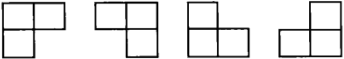
\includegraphics{lplate.png}\\
\figcaption{4种L型牌}\label{fig:lplate}
\end{center}

\subsubsection{输入}
第一行包含一个整数T,表示有T组测试用例。

每一组测试用例占用一行,包含一个整数k。

\subsubsection{输出}
所需L型牌的总数

\subsubsection{样例输入}
\begin{Code}
3
1
2
3
\end{Code}

\subsubsection{样例输出}
\begin{Code}
1
5
21
\end{Code}

\subsubsection{分析}
本题的棋盘是$2^k \times 2^k$,很容易想到用分治法。把棋盘切成4块,则每一块都是$2^{k-1} \times 2^{k-1}$的。有黑格的那一块可以递归解决,但其他3块并没有黑格子,应该怎么办呢?可以构造出一个黑格子,如图~\ref{fig:chessboard}所示,在中心放一个L型牌,其它3块也变成了子问题。递归边界不难得出,当$k=1$时1块L型牌就够了。
\begin{center}
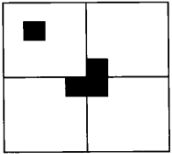
\includegraphics{chessboard.png}\\
\figcaption{棋盘覆盖问题的递归解法}\label{fig:chessboard}
\end{center}

本题只需要求总数,不需要求具体怎么摆放,因此简化很多。根据上面的思路,设$f(k)$表示棋盘是$2^k \times 2^k$时所需L型牌的总数,可得递推公式$f(k)=4f(k-1)+1$。

注意,$2^100$是一个很大的数,本题需要处理大数,见\S \ref{sec:bigintmul}节。

\subsubsection{代码}
\begin{Codex}[label=chessboard_cover.c]
#include<stdio.h>
#include<string.h>

#define MAXK 100

/* 一个数组元素表示4个十进制位,即数组是万进制的 */
#define BIGINT_MOD 10000
#define MOD_LEN 4
#define MAX_LEN (61/MOD_LEN+1)  /* 整数的最大位数, 10^x > 4^100 */

int  d[MAXK][MAX_LEN * 2];  /* d[k-1] = f(k) */

/**
 * @brief 打印大整数.
 * @param[in] x 大整数,用数组表示,低位在低地址
 * @param[in] n 数组x的长度
 * @return 无
 */
void bigint_print(const int x[], const int n) {
    int i;
    int start_output = 0;  /* 用于跳过前导0 */
    for (i = n - 1; i >= 0; --i) {
        if (start_output) {  /* 如果多余的0已经都跳过,则输出 */
            printf("%04d", x[i]);
        } else if (x[i] > 0) {
            printf("%d", x[i]);  /* 本题输出比较坑爹,最高位数字有前导0 */
            start_output = 1; /* 碰到第一个非0的值,就说明多余的0已经都跳过 */
        }
    }

    if(!start_output) printf("0");  /* 当x全为0时 */
}

/**
 * @brief 计算f(k) = 4f(k-1)+1,与大整数乘法很类似.
 * @param[in] x x
 * @param[in] y y
 * @param[out] z z=x*y+1
 * @return 无
 */
void bigint_mul_small(const int x[], const int y, int z[]) {
    int i;
    for (i = 0; i < MAX_LEN * 2; i++) z[i] = 0;

    z[0] = 1;

    for (i = 0; i < MAX_LEN; i++) z[i] += x[i] * y;
    
    for (i = 0; i < MAX_LEN * 2; i++) {  /* 统一处理进位问题 */
        if (z[i] >= BIGINT_MOD) {  /* 看是否要进位 */
            z[i+1] += z[i] / BIGINT_MOD;  /* 进位 */
            z[i] %= BIGINT_MOD;
        }
    }
}

int main() {
    int k, T;
    d[0][0] = 1;
    for (k = 2; k <= 100; k++) bigint_mul_small(d[k-2], 4, d[k-1]);

    scanf("%d", &T);
    while(T-- > 0) {
        scanf("%d", &k);
        bigint_print(d[k - 1], MAX_LEN * 2);
        printf("\n");
    }
    return 0;
}
\end{Codex}

\subsubsection{相关的题目}
与本题相同的题目:
\begindot
\item 《算法竞赛入门经典》\footnote{刘汝佳,算法竞赛入门经典,清华大学出版社,2009}第148页8.3.1节
\item 《计算机算法设计与分析(第3版)》\footnote{王晓东, 计算机算法设计与分析(第3版), 电子工业出版社, 2007}第19页2.6节
\item NYOJ 45 棋盘覆盖, \myurl{http://acm.nyist.net/JudgeOnline/problem.php?pid=45}
\myenddot

与本题相似的题目:
\begindot
\item POJ 2495 Incomplete chess boards, \myurl{http://poj.org/problem?id=2495}
\myenddot


\section{循环赛日程表} %%%%%%%%%%%%%%%%%%%%%%%%%%%%%%
\subsubsection{描述}
有$2^k$个运动员参加循环比赛,需要设计比赛日程表。要求如下:

\begindot
\item 每个选手必须与其他n-1个选手各赛一次
\item 每个选手一天只能赛一次
\item 比赛一共进行n-1天
\myenddot

按此要求设计一张比赛日程表,它有n行和n-1列,第i行第j列为第i个选手第j天遇到的对手。

\subsubsection{输入}
只有一个数k,$0<k<9$,且k为自然数。

\subsubsection{输出}
一张比赛日程表,它有n行和n-1列(不算第一列,第一列表示选手的编号),第i行第j列为第i个选手第j天遇到的对手。相邻的两个整数用空格隔开。

\subsubsection{样例输入}
\begin{Code}
1
\end{Code}

\subsubsection{样例输出}
\begin{Code}
1 2
2 1
\end{Code}

\subsubsection{分析}
根据分而治之的思想,可从其中一半选手($2^{k-1}$位)的比赛日程,推导出全体选手的日程,最终细分到只有两位选手的比赛日程。

图~\ref{fig:chessboard}所示是k=3时的一个可行解,它是由4块拼起来的。左上角是k=2时的一组解,左下角是由左上角每个数加4得到,而右上角、右下角分别由左下角、左上角复制得到。
\begin{center}
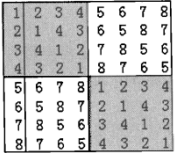
\includegraphics{roundrobin.png}\\
\figcaption{循环赛日程表问题k=3时的解}\label{fig:roundrobin}
\end{center}

\subsubsection{代码}
\begin{Codex}[label=roundrobin_scheduling.c]
#include<stdio.h>
#include<stdlib.h>

#define MAXN 512   /* N=2^k, 0<k9 */
short schedule[MAXN][MAXN];

void dc(const int k) {
    int i, j, t;
    int n, n2; /* 当前的n,即将扩展的n */

    /* k=1,即两个人时,日程表可以直接写出 */
    n=2;
    schedule[0][0]=1; schedule[0][1]=2;
    schedule[1][0]=2; schedule[1][1]=1;

     /* 迭代处理,依次处理2^2....2^k个选手的比赛日程 */
    for(t = 1; t < k; t++, n *= 2) {
        n2 = n * 2;
        //填左下角元素
        for(i = n; i < n2; i++)
            for(j = 0; j < n; j++)
                schedule[i][j] = schedule[i-n][j] + n;

        //将左下角元素抄到右上角
        for(i = 0; i < n; i++)
            for(j = n; j < n2; j++)
                schedule[i][j] = schedule[i+n][j-n];

        //将左上角元素抄到右下角
        for(i = n; i < n2; i++)
            for(j = n;j < n2; j++)
                schedule[i][j] = schedule[i-n][j-n];
    }
}

/* 另一个版本 */
void dc2(const int k) {
    int i, j, r;
    int n;
    const int N = 1 << k;

    /* 第一列是选手的编号 */
    for(i = 0; i < N; i++) schedule[i][0] = i + 1;
    schedule[0][1] = 1;  /* 当 k=0时,只有一个人 */

    for (n = 2; n <= N; n *= 2) {  /* 方块大小, 2, 4, 8 */
        const int half = n / 2;
        for (r = 0; r < N; r += n) { /* 方块所在行 */
            for (i = r; i <= r + half -1; i++) {  /* 左上角小方块的所有行 */
                for (j = 0; j < half; j++) {  /* 左上角小方块的所有行 */
                    /* 右下角 <-- 左上角 */
                    schedule[i + half][j + half] = schedule[i][j];
                    /* 右上角 <-- 左下角 */
                    schedule[i][j + half] = schedule[i + half][j];
                }
            }
        }
    }
}


int main(){
    int k, N;
    int i,j;

    scanf("%d",&k);
    N = 1 << k;

    dc(k);
    // dc2(k);

    // 输出日程表
    for(i = 0; i < N; i++) {
        for(j = 0; j < N; j++) printf("%d ", schedule[i][j]);
        printf("\n");
    }
    return 0;
}
\end{Codex}

\subsubsection{相关的题目}
与本题相同的题目:
\begindot
\item 《算法竞赛入门经典》\footnote{刘汝佳,算法竞赛入门经典,清华大学出版社,2009}第149页8.3.2节
\item 《计算机算法设计与分析(第3版)》\footnote{王晓东, 计算机算法设计与分析(第3版), 电子工业出版社, 2007}第34页2.11节
\item NKOJ 1437 校长杯, \myurl{http://acm.nankai.edu.cn/p1437.html}
\myenddot

与本题相似的题目:
\begindot
\item SPOJ 2826 Round-Robin Scheduling, \myurl{http://www.spoj.com/problems/RRSCHED/}
\item UVa OJ 678 Schedule of Taiwan Baseball League, \myurl{http://t.cn/zHJD9TQ}
\myenddot

\chapter{贪心法}
我们前面见过的一些算法,比如单源最短路径、最小生成树等都属于贪心法(greedy algorithm)。

如果一个问题具有以下两个要素:
\begindot
\item 最优子结构(optimal substructure)
\item 贪心选择性质(greedy-choice property)
\myenddot
则可以用贪心法求最优解。


\section{最优装载} %%%%%%%%%%%%%%%%%%%%%%%%%%%%%%


\section{哈弗曼编码} %%%%%%%%%%%%%%%%%%%%%%%%%%%%%%
\subsubsection{描述}
给定一个英文字符串,使用0和1对其进行编码,求最优前缀编码,使其所需要的比特数最少。

\subsubsection{分析}
题目很长,不过就是哈弗曼编码。

\subsubsection{代码}
\begin{Codex}[label=poj1521_entropy.cpp]
// 本题考查哈弗曼编码,但只需要统计哈弗曼编码后的总码长即可,
// 没必要建哈弗曼树得出哈弗曼编码
#include <stdio.h>
#include <string.h>
#include <queue>
#include <functional>

const int LINE_MAX = 256; // 一行最大字符数
const int MAX_ASCII = 128; // ASCII码最大值

int main_entropy() {
    char    s[LINE_MAX];
    int     count[MAX_ASCII] = {0}; // count[i]记录ASCII码为i的字符的出现次数
    int     sum;
    // 小根堆,队列头为最小元素
    priority_queue<int, vector<int>, greater<int> >    pq;

    while (scanf("%s", s) > 0) {
        sum = 0; // 清零
        const int len = strlen(s);

        if (strcmp(s,"END") == 0) {
            break;
        }

        for (int i = 0; i < len; i++) {
            count[s[i]]++;
        }

        for (int i = 0;i < MAX_ASCII; i++) {
            if (count[i] > 0) {
                pq.push(count[i]);
                count[i] = 0;
            }
        }
        while (pq.size() > 1) {
            const int a = pq.top(); pq.pop();
            const int b = pq.top(); pq.pop();
            sum += a + b; 
            pq.push(a + b);
        }
        if (sum == 0) {
            sum = len; // 此时pq中只有一个元素
        }
        
        while (!pq.empty()) { // clear
            pq.pop();
        }
        // 注意精度设置
        printf("%d %d %.1f\n", 8 * len, sum, ((double)8 * len) / sum);
    }
    return 0;
}
\end{Codex}

\subsubsection{相关的题目}
与本题相同的题目:
\begindot
\item POJ 1521 Entropy, \myurl{http://poj.org/problem?id=1521}
\myenddot

与本题相似的题目:
\begindot
\item  POJ 3253 Fence Repair, \myurl{http://poj.org/problem?id=3253}
\item 《算法竞赛入门经典》\footnote{刘汝佳,算法竞赛入门经典,清华大学出版社,2009} 第155页例题8-5
\item  《Introduction to Algorithms》\footnote{CLRS,Introduction to Algorithms(3rd Edition), 2009} 第16.3节
\item 《算法设计与分析(第3版)》\footnote{王晓东,计算机算法设计与分析(第3版), 2007} 第109页4.4节
\myenddot


\section{部分背包问题} %%%%%%%%%%%%%%%%%%%%%%%%%%%%%%

\chapter{动态规划}

【动态规划】

动态规划过程是:每次决策依赖于当前状态,又随即引起状态的转移。一个决策序列就是在变化的状态中产生出来的,所以,这种多阶段最优化决策解决问题的过程就称为动态规划。

【基本思想与策略】

基本思想与分治法类似,也是将待求解的问题分解为若干个子问题(阶段),按顺序求解子阶段,前一子问题的解,为后一子问题的求解提供了有用的信息。在求解任一子问题时,列出各种可能的局部解,通过决策保留那些有可能达到最优的局部解,丢弃其他局部解。依次解决各子问题,最后一个子问题就是初始问题的解。

由于动态规划解决的问题多数有重叠子问题这个特点,为减少重复计算,对每一个子问题只解一次,将其不同阶段的不同状态保存在一个二维数组中。

与分治法最大的差别是:适合于用动态规划法求解的问题,经分解后得到的子问题往往不是互相独立的(即下一个子阶段的求解是建立在上一个子阶段的解的基础上,进行进一步的求解)。

【适用的情况】

动态规划求最优解,适用于具有以下两个要素的优化问题:
\begindot
\item 最优子结构(optimal substructure):如果问题的最优解所包含的子问题的解也是最优的,就称该问题具有最优子结构,即满足最优化原理。
\item 无后续性:即某阶段状态一旦确定,就不受这个状态以后决策的影响。也就是说,某状态以后的过程不会影响以前的状态,只与当前状态有关。
\item 重叠子问题(overlap subproblem):即子问题之间是不独立的,一个子问题在下一阶段决策中可能被多次使用到。(该性质并不是动态规划适用的必要条件,但是如果没有这条性质,动态规划算法同其他算法相比就不具备优势)
\myenddot

【求解的基本步骤】

动态规划分为4个步骤:

动态规划所处理的问题是一个多阶段决策问题,一般由初始状态开始,通过对中间阶段决策的选择,达到结束状态。这些决策形成了一个决策序列,同时确定了完成整个过程的一条活动路线(通常是求最优的活动路线)。
动态规划的设计都有着一定的模式,一般要经历以下几个步骤。
初始状态→│决策1│→│决策2│→…→│决策n│→结束状态

(1)划分阶段:按照问题的时间或空间特征,把问题分为若干个阶段。在划分阶段时,注意划分后的阶段一定要是有序的或者是可排序的,否则问题就无法求解。

(2)确定状态和状态变量:将问题发展到各个阶段时所处于的各种客观情况用不同的状态表示出来。当然,状态的选择要满足无后效性。

(3)确定决策并写出状态转移方程:因为决策和状态转移有着天然的联系,状态转移就是根据上一阶段的状态和决策来导出本阶段的状态。所以如果确定了决策,状态转移方程也就可写出。但事实上常常是反过来做,根据相邻两个阶段的状态之间的关系来确定决策方法和状态转移方程。

(4)寻找边界条件:给出的状态转移方程是一个递推式,需要一个递推的终止条件或边界条件。

一般,只要解决问题的阶段、状态和状态转移决策确定了,就可以写出状态转移方程(包括边界条件)。

实际应用中可以按以下几个简化的步骤进行设计:

(1)分析最优解的性质,并刻画其结构特征。

(2)递归的定义最优解。

(3)以自底向上或自顶向下的记忆化方式(备忘录法)计算出最优值

(4)根据计算最优值时得到的信息,构造问题的最优解

【算法实现的说明】

动态规划的主要难点在于理论上的设计,也就是上面4个步骤的确定,一旦设计完成,实现部分就会非常简单。

使用动态规划求解问题,最重要的就是确定动态规划三要素:

(1)问题的阶段 

(2)每个阶段的状态

(3)从前一个阶段转化到后一个阶段之间的递推关系。

递推关系必须是从次小的问题开始到较大的问题之间的转化,从这个角度来说,动态规划往往可以用递归程序来实现,不过因为递推可以充分利用前面保存的子问题的解来减少重复计算,所以对于大规模问题来说,有递归不可比拟的优势,这也是动态规划算法的核心之处。

确定了动态规划的这三要素,整个求解过程就可以用一个最优决策表来描述,最优决策表是一个二维表,其中行表示决策的阶段,列表示问题状态,表格需要填写的数据一般对应此问题的在某个阶段某个状态下的最优值(如最短路径,最长公共子序列,最大价值等),填表的过程就是根据递推关系,从1行1列开始,以行或者列优先的顺序,依次填写表格,最后根据整个表格的数据通过简单的取舍或者运算求得问题的最优解。
$$f(n,m)=max{f(n-1,m), f(n-1,m-w[n])+P(n,m)}$$

写代码实现时有两种方式,“递归(recursive)+自顶向下(top-down)+表格”和
“自底向上(bottom-up)+表格”。前者属于一种 memorization (备忘录法),后者才是正宗的动规。

动规用表格将各个子问题的最优解存起来,避免重复计算,是一种空间换时间。

【动规 vs 贪心】

相同点:最优子结构。

不同点:
\begindot
\item[1]动规的子问题是重叠的,而贪心的子问题是不重叠的(disjoint subproblems);
\item[2]动规不具有贪心选择性质;
\item[3]贪心的前进路线是一条线,而动规是一个DAG。
\myenddot

分治和贪心的相同点:disjoint subproblems。

【动态规划算法基本框架】

\begin{Code}
	for(int j=1; j<=m; j=j+1) // 第一个阶段
		xn[j] = 初始值;
	
	for(int i=n-1; i>=1; i=i-1)// 其他n-1个阶段
		for(j=1; j>=f(i); j=j+1)//f(i)与i有关的表达式
			xi[j]=j=max(或min){g(xi-1[j1:j2]), ......, g(xi-1[jk:jk+1])};
	
	t = g(x1[j1:j2]); // 由子问题的最优解求解整个问题的最优解的方案
	
	print(x1[j1]);
	
	for(int i=2; i<=n-1; i=i+1){  
		t = t-xi-1[ji];
		
		for(j=1; j>=f(i); j=j+1)
			if(t=xi[ji]) break;
	}
\end{Code}

\section{动规和备忘录法的区别} %%%%%%%%%%%%%%%%%%%%%%%%%%%%%%
\label{sec:dp-vs-memorization}

动规(dynamic programming)一定是自底向上的,备忘录法(memorization)一定是自顶向下的。

动规不是lazy的, memorization 是lazy的,是按需(on-demand)计算的。所以,如果所有的子问题至少会碰到一次,则动规有优势;如果有些子问题在搜索过程中不会被碰到(即有剪枝),则 memorization 有优势。更详细的解释请参考StackOverflow上的这个帖子 \myurl{http://t.cn/z80ZS6B} 。

备忘录法可以实现跟动规类似的功能,但它不是动规。两者的方向是反的,一个是自顶向下,一个自底向上,我们应该区分开这两个概念。本书后面提到的动规,都是指自底向上的动规。

\section{动态规划与迭代法}
总结下:

1)递归能写出比较清晰简单的代码,但是有比较高的时间复杂度;

2)在递归不满足条件的情况下,动态规划是个比较好的选择;

3)一般来说,独立变量的个数决定动态规划的维度,例如l1和l2独立变化,所以用了二维动态规划。

\section{最长公共子序列} %%%%%%%%%%%%%%%%%%%%%%%%%%%%%%
\subsubsection{描述}
一个序列的子序列(subsequence)是指在该序列中删去若干(可以为0个)元素后得到的序列。
准确的说,若给定序列$X=(x_1,x_2,\cdots,x_m)$,则另一个序列$Z=(z_1,z_2,\cdots,z_k)$,
是X的子序列是指存在一个严格递增下标序列$(i_1,i_2,\cdots,i_k)$使得对于所有$j=1,2,\cdots,k$
有$z_j=x_{i_j}$。例如,序列$Z=(B,C,D,B)$是序列$X=(A,B,C,B,D,A,B)$的子序列,相应的
递增下标序列为$(1,2,4,6)$。

给定两个序列X和Y,求X和Y的最长公共子序列(longest common subsequence)。

\subsubsection{输入}
输入包括多组测试数据,每组数据占一行,包含两个字符串(字符串长度不超过200),代表两个序列。
两个字符串之间由若干个空格隔开。

\subsubsection{输出}
对每组测试数据,输出最大公共子序列的长度,每组一行。

\subsubsection{样例输入}
\begin{Code}
abcfbc abfcab
programming contest 
abcd mnp
\end{Code}

\subsubsection{样例输出}
\begin{Code}
4
2
0
\end{Code}

\subsubsection{分析}
最长公共子序列问题具有最优子结构性质。
设序列$X=(x_1,x_2,\cdots,x_m)$和$Y=(y_1,y_2,\cdots,y_n)$的最长公共子序列为$Z=(z_1,z_2,\cdots,z_k)$,则
\begindot
\item 若$x_m=y_n$,则$z_k=x_m=y_n$,且$Z_{k-1}$是$X_{m-1}$和$Y_{n-1}$的最长公共子序列。
\item 若$x_m \neq y_n$且$z_k \neq x_m$,则Z是$X_{m-1}$和$Y$的最长公共子序列。
\item 若$x_m \neq y_n$且$z_k \neq y_n$,则Z是$X$和$Y_{n-1}$的最长公共子序列。
\myenddot
其中,$X_{m-1}=(x_1,x_2,\cdots,x_{m-1})$, $Y_{n-1}=(y_1,y_2,\cdots,y_{n-1})$, $Z_{k-1}=(z_1,z_2,\cdots,z_{k-1})$。

设状态为d[i][j],表示序列$X_i$和$Y_j$的最长公共子序列的长度。由最优子结构可得状态转移方程如下:
$$
d[i][j]=\begin{cases}
0 & i=0,j=0\\
d[i-1][j-1]+1 & i,j>0; x_i=y_i \\
\max\left\{d[i][j-1],d[i-1][j]\right\} & i,j>0; x_i \neq y_i
\end{cases}
$$

如果要打印出最长公共子序列,需要另设一个数组p,p[i][j]记录d[i][j]是由哪个子问题得到的。

\subsubsection{代码}
\begin{Codex}[label=lcs.c]
#include <stdio.h>
#include <string.h>

#define MAX 201  /* 字符串最大长度为200 */

int d[MAX][MAX]; /* d[i][j]表示序列Xi和Yj的最长公共子序列的长度 */
char x[MAX], y[MAX];  /* 字符串末尾有个'0' */

void lcs(const char *x, const int m, const char *y, const int n) {
    int i, j;
    
    for (i = 0; i <= m; i++) d[i][0] = 0;  /* 边界初始化 */
    for (j = 0; j <= n; j++) d[0][j] = 0;

    for (i = 1; i <= m; i++) {
        for (j = 1; j <= n; j++) {
            if (x[i-1] == y[j-1]) {
                d[i][j] = d[i-1][j-1] + 1;
            } else {
                d[i][j] = d[i-1][j] > d[i][j-1] ? d[i-1][j] : d[i][j-1];
            }
        }
    }
}

void lcs_extend(const char *x, const int m, const char *y, const int n);
void lcs_print(const char *x, const int m, const char *y, const int n);

int main() {
    /* while (scanf ("%s%s", a, b)) { /* TLE */
    /* while (scanf ("%s%s", a, b) == 2) {  /* AC */
    while (scanf ("%s%s", x, y) != EOF) { /* AC */
        const int lx = strlen(x);
        const int ly = strlen(y);
        lcs(x, lx, y, ly);
        printf ("%d\n", d[lx][ly]);
        /*
        lcs_extend(x, lx, y, ly);
        lcs_print(x, lx, y, ly);
        printf("\n"); */
    }
    return 0;
}

int p[MAX][MAX]; /* p[i][j]记录d[i][j]是由哪个子问题得到的 */

void lcs_extend(const char *x, const int m, const char *y, const int n) {
    int i, j;
    
    memset(p, 0, sizeof(p));
    for (i = 0; i <= m; i++) d[i][0] = 0;  /* 边界初始化 */
    for (j = 0; j <= n; j++) d[0][j] = 0;

    for (i = 1; i <= m; i++) {
        for (j = 1; j <= n; j++) {
            if (x[i-1] == y[j-1]) {
                d[i][j] = d[i-1][j-1] + 1;
                p[i][j] = 1;
            } else {
                if (d[i-1][j] >= d[i][j-1]) {
                    d[i][j] = d[i-1][j];
                    p[i][j] = 2;
                } else {
                    d[i][j] = d[i][j-1];
                    p[i][j] = 3;
                }
            }
        }
    }
}

void lcs_print(const char *x, const int m, const char *y, const int n) {
    if (m == 0 || n == 0) return;

    if (p[m][n] == 1) {
        lcs_print(x, m - 1, y, n - 1);
        printf("%c", x[m - 1]);
    } else if (p[m][n] == 2) {
        lcs_print(x, m - 1, y, n);
    } else {
        lcs_print(x, m, y, n - 1);
    }
}
\end{Codex}

\subsubsection{相关的题目}
与本题相同的题目:
\begindot
\item 《计算机算法设计与分析(第3版)》\footnote{王晓东, 计算机算法设计与分析(第3版), 电子工业出版社, 2007}第56页3.3节
\item POJ 1458 Common Subsequence, \myurl{http://poj.org/problem?id=1458}
\item HDOJ 1159 Common Subsequence, \myurl{http://acm.hdu.edu.cn/showproblem.php?pid=1159}
\item 《程序设计导引及在线实践》\footnote{李文新,程序设计导引及在线实践, 清华大学出版社, 2007}第203页10.5节
\item 百练 2806 公共子序列, \myurl{http://poj.grids.cn/practice/2806/}
\myenddot

与本题相似的题目:
\begindot
\item HDOJ 1080 Human Gene Functions, \myurl{http://acm.hdu.edu.cn/showproblem.php?pid=1080}
\item HDOJ 1503 Advanced Fruits, \myurl{http://acm.hdu.edu.cn/showproblem.php?pid=1503}
\myenddot


\section{最大连续子序列和} %%%%%%%%%%%%%%%%%%%%%%%%%%%%%%
\subsubsection{描述}
给定一个整数序列$S_1,S_2,\cdot,S_n(1 \leq n \leq 1,000,000, -32768 \leq S_i \leq 32768)$,定义函数$sum(i,j)=S_i+\cdot+S_j(1 \leq i \leq j \leq n)$。

求最大的$sum(i,j)$,即\textbf{最大连续子序列和}(maximum continuous subsequence sum)。

\subsubsection{输入}
每个测试用例由正整数n开头,接着是n个整数。

\subsubsection{输出}
每行输出一个最大和。

\subsubsection{样例输入}
\begin{Code}
3 1 2 3
6 -1 4 -2 3 -2 3
\end{Code}

\subsubsection{样例输出}
\begin{Code}
6
6
\end{Code}

\subsubsection{分析}
当我们从头到尾遍历这个数组的时候,对于数组里的一个整数,它有几种选择呢?它只有两种选择: 1、加入之前的SubArray;2. 自己另起一个SubArray。那什么时候会出现这两种情况呢?

如果之前SubArray的总体和大于0的话,我们认为其对后续结果是有贡献的。这种情况下我们选择加入之前的SubArray

如果之前SubArray的总体和为0或者小于0的话,我们认为其对后续结果是没有贡献,甚至是有害的(小于0时)。这种情况下我们选择以这个数字开始,另起一个SubArray。

设状态为d[j],表示以S[j]结尾的最大连续子序列和,则状态转移方程如下:
\begin{eqnarray}
d[j] &=& \max\left\{d[j-1]+S[j],S[j]\right\}, \text{ 其中 }1 \leq j \leq n \nonumber \\
target &=& \max\left\{d[j]\right\}, \text{ 其中 }1 \leq j \leq n \nonumber
\end{eqnarray}

解释如下:
\begindot
\item 情况一,S[j]不独立,与前面的某些数组成一个连续子序列,则最大连续子序列和为$d[j-1]+S[j]$。
\item 情况二,S[j]独立划分成为一段,即连续子序列仅包含一个数S[j],则最大连续子序列和为$S[j]$。
\myenddot    

\subsubsection{代码}
\begin{Codex}[label=mcss.c]
#include <stdio.h>
#include <stdlib.h>
#include <limits.h>

#define max(a,b) ((a)>(b)?(a):(b))
#define min(a,b) ((a)<(b)?(a):(b))

/**
 * @brief 最大连续子序列和,思路四
 * @param[in] S 数列
 * @param[in] n 数组的长度
 * @return 最大连续子序列和
 */
int mcss(int S[], int n) {
    int i, result, cur_min;
    int *sum = (int*) malloc((n + 1) * sizeof(int));  // 前n项和

    sum[0] = 0;
    result = INT_MIN;
    cur_min = sum[0];
    for (i = 1; i <= n; i++) { /* 变成前缀和 */
        sum[i] = sum[i - 1] + S[i - 1];
    }
    for (i = 1; i <= n; i++) {
        result = max(result, sum[i] - cur_min);
        cur_min = min(cur_min, sum[i]);
    }
    free(sum);
    return result;
}

/**
 * @brief 最大连续子序列和,动规
 * @param[in] S 数列
 * @param[in] n 数组的长度
 * @return 最大连续子序列和
 */
int mcss_dp(int S[], int n) {
    int i, result;
    int *d = (int*) malloc(n * sizeof(int));
    d[0] = S[0];
    result = d[0];
    for (i = 1; i < n; i++) {
        d[i] = max(S[i], d[i - 1] + S[i]);
        if (result < d[i])
            result = d[i];
    }
    free(d);
    return result;
}

int main() {
    int n, *S;
    while (scanf("%d", &n) > 0) {
        int i;
        S = (int*) malloc(n * sizeof(int));
        for (i = 0; i < n; i++)
            scanf("%d", &S[i]);

        printf("%d\n", mcss_dp(S, n));
        free(S);
    }
    return 0;
}
\end{Codex}

\subsubsection{其他解法}

\begindot
\item 思路一:直接在i到j之间暴力枚举,复杂度是$O(n^3)$
\item 思路二:处理后枚举,连续子序列的和等于两个前缀和之差,复杂度$O(n^2)$。
\item 思路三:分治法,把序列分为两段,分别求最大连续子序列和,然后归并,复杂度$O(n\log n)$
\item 思路四:把$O(n^2)$的代码稍作处理,得到$O(n)$的算法
\item 思路五:M=1的最大M子段和,见第 \S \ref{sec:mmss} 节
\myenddot

感兴趣的读者请参考这篇博客,\myurl{http://www.cnblogs.com/gj-Acit/archive/2013/02/12/2910332.html}

\subsubsection{相关题目}
与本题相同的题目:
\begindot
\item LeetCode Maximum Subarray, \myurl{http://leetcode.com/onlinejudge\#question_53}
\myenddot

与本题相似的题目:
\begindot
\item HDOJ 1024 Max Sum Plus Plus, \myurl{http://acm.hdu.edu.cn/showproblem.php?pid=1024}
\myenddot


\section{Minimum Adjustment Cost}
\subsubsection{描述}
Given an integer array, adjust each integers so that the difference of every 
adjcent integers are not greater than a given number target.

If the array before adjustment is A, the array after adjustment is B, you 
should minimize the sum of |A[i]-B[i]|.

注意
You can assume each number in the array is a positive integer and not greater 
than 100

\subsubsection{输入}
An integer array vector<int> A and a target

\subsubsection{输出}
minimize the sum of |A[i]-B[i]|

\subsubsection{样例输入}
\begin{Code}
	[1,4,2,3], 1
\end{Code}

\subsubsection{样例输出}
\begin{Code}
	2
\end{Code}

\subsubsection{分析}
dp[i][j]: 把A[i]的值修改为j,所需要的最小花费, 则dp[i][j] = min\{dp[i-1][k] + 
	|j-A[i]|\}  s.t. |k-j| <= target

\subsubsection{代码}
\begin{Codex}[label=MinAdjustmentCost.c]
	#define MAXTARGET 100
	
	int MinAdjustmentCost(vector<int> A, int target) {
		if (A.empty()) 
		return 0;
		int cur = 0;
		// dp[i][j]: 把A[i]的值修改为j,所需要的最小花费, 则dp[i][j] = min{dp[i-1][k] 
			+ |j-A[i]|}  s.t. |k-j| <= target
		int dp[2][MAXTARGET + 1];
		memset(dp, 0x00, sizeof(dp));
		
		for (int i = 0; i < A.size(); i++) {
			int next = cur ^ 1;
			for (int j = 1; j <= MAXTARGET; j++) {
				dp[next][j] = INT_MAX;
				for (int k = max(j-target, 1); k <= min(MAXTARGET, j+target); 
				k++)
				dp[next][j] = min(dp[next][j], dp[cur][k] + abs(A[i]-j));
			}
			cur ^= 1;
		}
		int ans = INT_MAX;
		for (int i = 1; i <= MAXTARGET; i++)
		ans = min(ans, dp[cur][i]);
		
		return ans;
	}
\end{Codex}

\subsubsection{相关的题目}
与本题相同的题目:
\begindot
\item POJ 3494 Largest Submatrix of All 1's, 
\myurl{http://poj.org/problem?id=3494}
\item LeetCode Maximal Rectangle, 
\myurl{http://leetcode.com/onlinejudge\#question_85},\\ 
参考代码\myurl{https://gist.github.com/soulmachine/b20a15009450016038d9}
\myenddot

与本题相似的题目:
\begindot
\item Vijos 1055 奶牛浴场, \myurl{https://vijos.org/p/1055}
\myenddot

\section{最大M子段和} %%%%%%%%%%%%%%%%%%%%%%%%%%%%%%
\label{sec:mmss}

\subsubsection{描述}
给定一个整数序列$S_1,S_2,\cdot,S_n(1 \leq n \leq 1,000,000, -32768 \leq S_i \leq 32768)$,定义函数$sum(i,j)=S_i+ ... +S_j(1 \leq i \leq j \leq n)$。

现给定一个正整数m,找出m对i和j,使得$sum(i_1,j_1)+sum(i_2,j_2)+ ... +sum(i_m,j_m)$最大。这就是\textbf{最大M子段和}(maximum m segments sum)。

\subsubsection{输入}
每个测试用例由两个正整数m和n开头,接着是n个整数。

\subsubsection{输出}
每行输出一个最大和。

\subsubsection{样例输入}
\begin{Code}
1 3 1 2 3
2 6 -1 4 -2 3 -2 3
\end{Code}

\subsubsection{样例输出}
\begin{Code}
6
8
\end{Code}

\subsubsection{分析}
设状态为d[i,j],表示前j项分为i段的最大和,且第i段必须包含S[j],则状态转移方程如下:
\begin{eqnarray}
d[i,j] &=& \max\left\{d[i,j-1]+S[j],\max\left\{d[i-1,t]+S[j]\right\}\right\}, \text{ 其中 }i \leq j \leq n, i-1 \leq t < j \nonumber \\
target &=& \max\left\{d[m,j]\right\}, \text{ 其中 }m \leq j \leq n \nonumber
\end{eqnarray}

分为两种情况:
\begindot
\item 情况一,S[j]包含在第i段之中,$d[i,j-1]+S[j]$。
\item 情况二,S[j]独立划分成为一段,$\max\left\{d[i-1,t]+S[j]\right\}$。
\myenddot

观察上述两种情况可知d[i,j]的值只和d[i,j-1]和d[i-1,t]这两个值相关,因此不需要二维数组,可以用滚动数组,只需要两个一维数组,用d[j]表示现阶段的最大值,即$d[i,j-1]+S[j]$,用prev[j]表示上一阶段的最大值,即$\max\left\{d[i-1,t]+S[j]\right\}$。

\subsubsection{代码}
\begin{Codex}[label=mmss.c]
#include <stdio.h>
#include <stdlib.h>
#include <limits.h>

/**
 * @brief 最大m段子序列和
 * @param[in] S 数组
 * @param[in] n 数组长度
 * @param[in] m m段
 * @return 最大m段子序列和
 */
int mmss(int S[], int n, int m) {
    int max_sum, i, j;

    /* d[i]表示现阶段最大值,prev[i]表示上阶段最大值 */
    /* d[0], prev[0] 未使用 */
    int *d = (int*) calloc(n + 1, sizeof(int));
    int *prev = (int*) calloc(n + 1, sizeof(int));
    S--;  // 因为 j是从1开始,而S从0开始,这里要减一

    for (i = 1; i <= m; ++i) {
        max_sum = INT_MIN;
        for (j = i; j <= n; ++j) {
            // 状态转移方程
            if (d[j - 1] < prev[j - 1])
                d[j] = prev[j - 1] + S[j];
            else
                d[j] = d[j - 1] + S[j];

            prev[j - 1] = max_sum;  // 存放上阶段最大值
            if (max_sum < d[j])
                max_sum = d[j];  // 更新 max_sum
        }
        prev[j - 1] = max_sum;
    }

    free(d);
    free(prev);
    return max_sum;
}

int main() {
    int n, m, i, *S;
    while (scanf("%d%d", &m, &n) == 2) {
        S = (int*) malloc(sizeof(int) * n);
        for (i = 0; i < n; ++i)
            scanf("%d", &S[i]);
        printf("%d\n", mmss(S, n, m));
        free(S);
    }
    return 0;
}
\end{Codex}

\subsubsection{相关题目}
与本题相同的题目:
\begindot
\item HDOJ 1024 Max Sum Plus Plus, \myurl{http://acm.hdu.edu.cn/showproblem.php?pid=1024}
\myenddot

与本题相似的题目:
\begindot
\item LeetCode Best Time to Buy and Sell Stock III, \myurl{http://leetcode.com/onlinejudge\#question_123},\\
参考代码\myurl{https://gist.github.com/soulmachine/5906637}
\myenddot


\section{背包问题} %%%%%%%%%%%%%%%%%%%%%%%%%%%%%%
背包问题(Knapsack problem\footnote{Knapsack problem, \myurl{http://en.wikipedia.org/wiki/Knapsack_problem}})
有很多种版本,常见的是以下三种:
\begindot
\item 0-1背包问题(0-1 knapsack problem):每种物品只有一个
\item 完全背包问题(UKP, unbounded knapsack problem):每种物品都有无限个可用
\item 多重背包问题(BKP, bounded knapsack problem):第i种物品有c[i]个可用
\myenddot

其他版本的背包问题请参考“背包问题九讲”,\myurl{https://github.com/tianyicui/pack}

背包问题是一种“多阶段决策问题”。

\subsection{0-1背包问题}

\subsubsection{描述}
有$N$种物品,第$i$种物品的重量为$w_i$,价值为$v_i$,每种物品只有一个。背包能承受的重量为$W$。
将哪些物品装入背包可使这些物品的总重量不超过背包容量,且价值总和最大?

\subsubsection{输入}
第1行包含一个整数T,表示有T组测试用例。
每组测试用例有3行,第1行包含两个整数$N, W(N \leq 1000 , W \leq 1000)$分别表示
物品的种数和背包的容量,第2行包含N个整数表示每种物品的价值,第3行包含N个整数表示每种物品的重量。

\subsubsection{输出}
每行一个整数,表示价值总和的最大值。

\subsubsection{样例输入}
\begin{Code}
1
5 10
1 2 3 4 5
5 4 3 2 1
\end{Code}

\subsubsection{样例输出}
\begin{Code}
14
\end{Code}

\subsubsection{分析}
由于每种物品仅有一个,可以选择装或者不装。

定义状态f[i][j],表示“把前i个物品装进容量为j的背包可以获得的最大价值”,
则其状态转移方程便是:
$$f[i][j]=\max\left\{f[i-1][j], f[i-1][j-w[i]+v[i]\right\}$$

这个方程理解如下,把前i个物品装进容量为j的背包时,有两种情况:
\begindot
\item 第i个不装进去,这时所得价值为:$f[i-1][j]$
\item 第i个装进去,这时所得价值为:$f[i-1][j-w[i]]+v[i]$
\myenddot

动规过程的伪代码如下:
\begin{Code}
f[0..N][0..W] = 0
for i=1..N
    for j=0..W
        f[i][j]=max{f[i-1][j],f[i-1][j-w[i]]+v[i]};
\end{Code}

内循环从右向左也可以:
\begin{Code}
f[0..N][0..W] = 0
for i=1..N
    for j=W..0
        f[i][j]=max{f[i-1][j],f[i-1][j-w[i]]+v[i]};
\end{Code}

内循环从右向左时,可以把二维数组优化成一维数组。伪代码如下:
\begin{Code}
for i=1..N
    for j=W..0
        d[j]=max{d[j],d[j-w[i]]+v[i]};
\end{Code}

为什么呢?举个例子,测试数据如下:
\begin{Code}
1
3 10
4 5 6
3 4 5
\end{Code}

f是从上到下、从右到左计算的,如图~\ref{fig:01knapsack}所示。
\begin{center}
\includegraphics[width=360pt]{01knapsack.gif}\\
\figcaption{0-1背包问题的计算顺序}\label{fig:01knapsack}
\end{center}

当内循环是逆序时,且动规是用自底向上方式实现时,就可以保证同一行可以从右向左更新。

设一维数组为d(又称为滚动数组\footnote{刘汝佳,算法竞赛入门经典,清华大学出版社,2009,第169页9.3.3节}),
在更新d[j]之前,d[j]里保存的f[i-1][j],更新之后,d[j]里保存的是f[i][j]。

事实上,使用一维数组解0-1背包问题的程序在后面会被多次用到,所以这里抽象出一
个处理单个物品的函数,以后的代码中直接调用不加说明。
\begin{Code}
def ZeroOneKnapsack(d[], i)
    for j = W..w[i]
        d[j] = max(d[j], d[j-w[i]] + v[i])
\end{Code}

有了这个函数以后,0-1背包问题的伪代码就可以这样写:
\begin{Code}
d[0..W] = 0
for i = 1..N
    ZeroOneKnapsack(d[], i)
\end{Code}

\subsubsection{代码}
版本1,自底向上。

\begin{Codex}[label=01knapsack.c]
#include <stdio.h>
#include <string.h>

#define MAXN 1000
#define MAXW 1000

int N, W;
int w[MAXN+1], v[MAXN+1]; /* 0 没有用 */

int f[MAXN + 1][MAXW + 1];

void dp() {
    int i, j;
    memset(f, 0, sizeof(f)); /* 背包不一定要装满 */
    for(i = 1; i <= N; ++i) {
        /* for(j = W; j >= 0; --j) { /* 也可以 */
        for(j = 0; j <= W; ++j) {
            f[i][j] = f[i-1][j];
            if(j >= w[i]) {
                const int tmp = f[i-1][j-w[i]] + v[i];
                if(tmp > f[i][j]) f[i][j] = tmp;
            }
        }
    }
}

int main() {
    int i, T;
    scanf("%d", &T);
    while(T--) {
        scanf("%d %d", &N, &W);
        for(i = 1; i <= N; ++i) scanf("%d", &v[i]);
        for(i = 1; i <= N; ++i) scanf("%d", &w[i]);

        dp();
        printf("%d\n", f[N][W]);
    }
    return 0;
}
\end{Codex}

版本2,自底向上,滚动数组。

\begin{Codex}[label=01knapsack2.c]
#include <stdio.h>
#include <string.h>

#define MAXN 1000
#define MAXW 1000

int N, W;
int w[MAXN], v[MAXN];

int d[MAXW + 1]; /* 滚动数组 */

/**
 * @brief 0-1背包问题中,处理单个物品.
 * @param[in] d 滚动数组
 * @param[in] i 该物品的下标
 * @return 无
 */
void zero_one_knapsack(int d[], const int i) {
    int j;
    for(j = W; j >= w[i]; --j) {
        const int tmp = d[j - w[i]] + v[i];
        if(tmp > d[j]) d[j] = tmp; /* 求最小用 <,求最大用 > */
    }
}

void dp() {
    int i;
    memset(d, 0, sizeof(d)); /* 背包不一定要装满 */

    for(i = 0; i < N; ++i) zero_one_knapsack(d, i);
}

int main() {
    int i, T;
    scanf("%d", &T);
    while(T--) {
        scanf("%d %d", &N, &W);
        for(i = 0; i < N; ++i) scanf("%d", &v[i]);
        for(i = 0; i < N; ++i) scanf("%d", &w[i]);

        dp();
        printf("%d\n", d[W]);
    }
    return 0;
}
\end{Codex}

\subsubsection{相关的题目}
与本题相同的题目:
\begindot
\item 《算法竞赛入门经典》\footnote{刘汝佳,算法竞赛入门经典,清华大学出版社,2009}第167页例题9-5
\item  HDOJ 2602 Bone Collector, \myurl{http://acm.hdu.edu.cn/showproblem.php?pid=2602}
\myenddot

与本题相似的题目:
\begindot
\item  wikioi 1014 装箱问题, \myurl{http://www.wikioi.com/problem/1014/}, \\
参考代码 \myurl{https://gist.github.com/soulmachine/6248518}
\myenddot

\subsection{完全背包问题}
\label{sec:ukp}

\subsubsection{描述}
给你一个储钱罐(piggy bank),往里面存硬币。存入的过程是不可逆的,要想把钱拿出来只能摔碎
储钱罐。因此,你想知道里面是否有足够多的钱,把它摔碎是值得的。

你可以通过储钱罐的重量来推测里面至少有多少钱。已知储钱罐空的时候的重量和装了硬币后的重量,
还有每种硬币的重量和面值,每种硬币的数量不限。求在最坏情况下,储钱罐里最少有多少钱。

\subsubsection{输入}
第1行包含一个整数T,表示有T组测试用例。
每组测试用例,第一行是两个整数E和F,分别表示空储钱罐的重量和装了硬币后的重量,以克(gram)为单位,
储钱罐的重量不会超过10kg,即$1 \leq E \leq F \leq 10000$。第二行是一个整数$N(1 \leq N \leq 500)$,表示
硬币的种类数目。接下来是N行,每行包含两个整数v和w($1 \leq v \leq 50000, 1 \leq w \leq 10000$),分别
表示硬币的面值和重量。

\subsubsection{输出}
每个案例打印一行。内容是"The minimum amount of money in the piggy-bank is X.",其中
X表示储钱罐里最少有多少钱。如果不能精确地达到给定的重量,则打印"This is impossible."。

\subsubsection{样例输入}
\begin{Code}
3
10 110
2
1 1
30 50
10 110
2
1 1
50 30
1 6
2
10 3
20 4
\end{Code}

\subsubsection{样例输出}
\begin{Code}
The minimum amount of money in the piggy-bank is 60.
The minimum amount of money in the piggy-bank is 100.
This is impossible.
\end{Code}

\subsubsection{分析}
每种物品有无限个可用,这是完全背包问题。

本题没有给出储钱罐的容量,但每个案例给出了,初始为空时的重量E和装了硬币后的重量F,
因此可以把储钱罐看作一个容量为F-E的背包,背包必须要装满。

这个问题非常类似于0-1背包问题,所不同的是每种物品有无限个。也就是从每种
物品的角度考虑,与它相关的策略已并非取或不取两种,而是取0个、取1个、取2
个……直至取$W/w[i]$个。

一种好想好写的基本方法是转化为0-1背包问题:把第i种物品换成$W/w[i]$个0-1
背包问题中的物品,则得到了物品数为$\sum \dfrac{W}{w[i]}$的0-1背包问题。
时间复杂度是$O(W\sum \dfrac{W}{w[i]})$。

按照该思路,状态转移方程为:
$$f[i][j]=\max\left\{f[i-1][j-k*w[i]]+k*v[i], 0 \leq k*w[i] \leq j\right\}$$

伪代码如下:
\begin{Code}
for i = 1..N
    for j = W..w[i]
        for k = 1..j/w[i]
            d[j] = max{d[j], d[j-k*w[i]] + k*v[i]};
\end{Code}

也可以写成:
\begin{Code}
for i = 1..N
    for k = 1..W/w[i]
        ZeroOneKnapsack(d[], w, v)
\end{Code}

“拆分物品”还有更高效的拆分方法:把第i种物品拆分成重量为$2^k*w[i]$、价值为$2^k*v[i]$的
若干物品,其中k取所有满足$2^k*w[i] \leq W$的非负整数。这是二进制的思想,因为闭区间[1, W/w[i]]中
的任何整数都可以表示为$1, 2, 4, ..., 2^k$中若干个的和。

这样处理单个物品的复杂度由$O\left(\dfrac{W}{w[i]}\right)$降到了$O\left(\log \dfrac{W}{w[i]}\right)$,伪代码如下:
\begin{Code}
def UnboundedKnapsack(d[], i)
    k=1
    while k*w[i] <= W
        ZeroOneKnapsack(d[], k*w[i], k*v[i])
        k=2*k
\end{Code}

还存在更优化的算法,复杂度为$O(NW)$,伪代码如下:
\begin{Code}
for i = 1..N
    for j = 0..W
        d[j] = max{d[j], d[j-w[i]] + v[i]};
\end{Code}

与0-1背包问题相比,仅有一行代码不同,这里内循环是顺序的,而0-1背包是逆序的(在使用滚动数组的情况下)。

为什么这个算法可行呢?首先想想为什么0-1背包中内循环要逆序,逆序是为了保证每个物品只选一次,保证在
“选择第i件物品”时,依赖的是一个没有选择第i件物品的子结果$f[i-1][j-w[i]]$。而现在完全背
包的特点却是每种物品可选无限个,没有了每个物品只选一次的限制,所以就可以并且必须采用j递增
的顺序循环。

根据上面的伪代码,状态转移方程也可以写成这种形式:
$$f[i][j]=\max\left\{f[i-1][j], f[i][j-w[i]+v[i]\right\}$$

抽象出处理单个物品的函数:
\begin{Code}
def UnboundedKnapsack(d[], i)
    for j = w[i]..W
        d[j] = max(d[j], d[j-w[i]] + v[i])
\end{Code}

\subsubsection{代码}
\begin{Codex}[label=piggy_bank.c]
#include <stdio.h>

#define MAXN 500
#define MAXW 10000
 /* 无效值,不要用0x7FFFFFFF,执行加运算后会变成负数 */
const int INF = 0x0FFFFFFF;

int N, W;
int w[MAXN], v[MAXN];

int d[MAXW + 1]; /* 滚动数组 */

/**
 * @brief 完全背包问题中,处理单个物品.
 * @param[in] d 滚动数组
 * @param[in] i 该物品的下标
 * @return 无
 */
void unbounded_knapsack(int d[], const int i) {
    int j;
    for(j = w[i]; j <= W; ++j) {
        const int tmp = d[j - w[i]] + v[i];
        if(tmp < d[j]) d[j] = tmp; /* 求最小用 <,求最大用 > */
    }
}
/** c,物品的系数 */
void zero_one_knapsack(int d[], const int i, const int c) {
    int j;
    const int neww = c * w[i];
    const int newv = c * v[i];
    for(j = W; j >= neww; --j) {
        const int tmp = d[j - neww] + newv;
        if(tmp < d[j]) d[j] = tmp;  /* 求最小用 <,求最大用 > */
    }
}

void unbounded_knapsack1(int d[], const int i) {
    int k = 1;
    while(k * w[i] <= W) {
        zero_one_knapsack(d, i, k);
        k *= 2;
    }
}

void dp() {
    int i;
    for(i = 0; i <= W; ++i) d[i] = INF; /* 背包要装满 */
    d[0] = 0;

    for(i = 0; i < N; ++i) unbounded_knapsack(d, i);
}

int main() {    
    int i, T;
    int E, F;
 
    scanf("%d", &T);
    while(T--) {
        scanf("%d %d", &E, &F);
        W = F - E;
        scanf("%d", &N);
        for(i = 0; i < N; ++i) scanf("%d %d", &v[i], &w[i]);

        dp();
        if(d[W] == INF) {
            printf("This is impossible.\n");
        } else {
            printf("The minimum amount of money in the piggy-bank is %d.\n",
                    d[W]);
        }
    }
    return 0;
}

/* 将第i种物品取0个,1个,...,W/w[i]个,该版本不能AC,会TLE */
void unbounded_knapsack2(int d[], const int w, const int v) {
    int j, k;
    for(j = W; j >= w; --j) {
        const int K = j / w;
        for(k = 1; k <= K; ++k) {
            const int tmp = d[j - k * w] + k * v;
            if(tmp < d[j]) d[j] = tmp; /* 求最小用 <,求最大用 > */
        }
    }
}

/* 将第i种物品取0个,1个,...,W/w[i]个,该版本不能AC,会TLE */
void unbounded_knapsack3(int d[], const int w, const int v) {
    int k;
    const int K = W / w;
    for(k = 0; k < K; ++k){
        zero_one_knapsack(d, w, v);
    }
}
\end{Codex}

\subsubsection{相关的题目}
与本题相同的题目:
\begindot
\item 《算法竞赛入门经典》\footnote{刘汝佳,算法竞赛入门经典,清华大学出版社,2009}第167页例题9-4
\item POJ 1384 Piggy-Bank, \myurl{http://poj.org/problem?id=1384}
\item HDOJ 1114 Piggy-Bank, \myurl{http://t.cn/zWXbXIn}
\myenddot

与本题相似的题目:
\begindot
\item POJ 2063 Investment, \myurl{http://poj.org/problem?id=2063}
\myenddot

\subsection{多重背包问题}

\subsubsection{描述}
某地发生地震,为了挽救灾区同胞的生命,心系灾区同胞的你准备自己采购一些粮食
支援灾区,现在假设你一共有资金W元,而市场有N种大米,每种大米都是袋装产品,
其价格不等,并且只能整袋购买。

请问:你用有限的资金最多能采购多少公斤粮食呢?

\subsubsection{输入}
第1行包含一个整数T,表示有T组测试用例。
每组测试用例的第一行是两个整数W和N($1 \leq W \leq 100, 1 \leq N \leq 100$),分别表示经费的金
额和大米的种类,然后是N行数据,每行包含3个整数w,v和c
($1 \leq w \leq 20,1 \leq v \leq 200,1 \leq c \leq 20$),
分别表示每袋的价格、每袋的重量以及对应种类大米的袋数。

\subsubsection{输出}
对于每组测试用例,输出能够购买大米的最大重量,你可以假设经费买不光所有的大米,
并且经费你可以不用完。每个实例的输出占一行。

\subsubsection{样例输入}
\begin{Code}
1
8 2
2 100 4
4 100 2
\end{Code}

\subsubsection{样例输出}
\begin{Code}
400
\end{Code}

\subsubsection{分析}
第i种物品有c[i]个可用,这是多重背包问题。

与完全背包问题类似,也可以用“拆分物品”的思想把本问题转化为0-1背包问题:把
第i种物品换成$c[i]$个0-1背包问题中的物品,则得到了物品数为$\sum c[i]$的0-1背包问题。
时间复杂度是$O(W\sum c[i])$。状态转移方程为:
$$f[i][j]=\max\left\{f[i-1][j-k*w[i]]+k*v[i], 0 \leq k \leq c[i], 0 \leq k*w[i] \leq j\right\}$$

伪代码如下:
\begin{Code}
for i = 1..N
    for j = W..w[i]
        K = min{j/w[i], c[i]}
        for k = 1..K
            d[j] = max{d[j], d[j-k*w[i]] + k*v[i]};
\end{Code}

也可以写成:
\begin{Code}
for i = 1..N
    for k = 1..c[i]
        ZeroOneKnapsack(d[], i)
\end{Code}

拆分物品也可以使用二进制的技巧,把第i种物品拆分成若干物品,其中每件物品都有一个
系数,这个新物品的重量和价值均是原来的重量和价值乘以这个系数。系数分别为
$1,2,2^2,...,2^{k-1},c[i]-2^k+1$,其中k是满足$2^k-1<c[i]$的最大整数。例如,某种物品
有13个,即c[i]=13,则相应的k=3,这种物品应该被拆分成系数分别1,2,4,6的四个物品。

这样处理单个物品的复杂度由$O(c[i])$降到了$O(\log c[i])$,伪代码如下:
\begin{Code}
// c, 物品系数
def ZeroOneKnapsack(d[], i, c)
    for j = W..w[i]
        d[j] = max(d[j], d[j-c*w[i]] + c*v[i])
def BoundedKnapsack(d[], i)
    if c[i]*w[i] >= W
        unbounded_knapsack(d[], i);
        return;

    k = 1;
    while k < c[i]
        zero_one_knapsack(d[], i, k);
        c[i] -= k;
        k *= 2;

    zero_one_knapsack(d[], i, c);
\end{Code}

\subsubsection{代码}
\begin{Codex}[label=bkp.c]
#include <stdio.h>
#include <string.h>

#define MAXN 100
#define MAXW 100

int N, W;
int w[MAXN], v[MAXN], c[MAXN];

int d[MAXW + 1]; /* 滚动数组 */

/** c,物品的系数 */
void zero_one_knapsack(int d[], const int i, const int c) {
    int j;
    const int neww = c * w[i];
    const int newv = c * v[i];
    for(j = W; j >= neww; --j) {
        const int tmp = d[j - neww] + newv;
        if(tmp > d[j]) d[j] = tmp;  /* 求最小用 <,求最大用 > */
    }
}

void unbounded_knapsack(int d[], const int i) {
    int j;
    for(j = w[i]; j <= W; ++j) {
        const int tmp = d[j - w[i]] + v[i];
        if(tmp > d[j]) d[j] = tmp; /* 求最小用 <,求最大用 > */
    }
}

/**
 * @brief 多重背包问题中,处理单个物品.
 * @param[in] d 滚动数组
 * @param[in] i 该物品的下标
 * @param[in] c 该物品的数量
 * @return 无
 */
void bounded_knapsack(int d[], const int i) {
    int k;
    for(k = 0; k < c[i]; ++k) {
        zero_one_knapsack(d, i, 1);
    }
}

/* 另一个版本,拆分物品更加优化 */
void bounded_knapsack1(int d[], const int i) {
    int k;
    if(c[i] * w[i] >= W) {
        unbounded_knapsack(d, i);
        return;
    }

    k = 1;
    while(k < c[i]) {
        zero_one_knapsack(d, i, k);
        c[i] -= k;
        k *= 2;
    }
    zero_one_knapsack(d, i, c[i]);
}

void dp() {
    int i;
    memset(d, 0, sizeof(d)); /* 背包不一定要装满 */

    for(i = 0; i < N; ++i) bounded_knapsack1(d, i);
}
 
int main() {
    int i;
    int T;
    scanf("%d", &T);
    while(T--) {
        scanf("%d %d", &W, &N);
        for(i = 0; i < N; ++i) scanf("%d %d %d", &w[i], &v[i], &c[i]);

        dp();
        printf("%d\n", d[W]);
    }
    return 0;
}
\end{Codex}

\subsubsection{相关的题目}
与本题相同的题目:
\begindot
\item HDOJ 2191 买大米, \myurl{http://acm.hdu.edu.cn/showproblem.php?pid=2191}
\myenddot

与本题相似的题目:
\begindot
\item None
\myenddot


\section{序列型动态规划} %%%%%%%%%%%%%%%%%%%%%%%%%%%%%%
对于所有动规题目,如果把状态转移图画出来,一定是一个有向无环图(DAG)。再进一步细分类别,有序列型动态规划,棋盘型动态规划,树型动态规划等等。


\subsection{最长上升子序列}

\subsubsection{描述}
当一个序列严格递增时,我们称这个序列是上升的。
对于一个给定的序列$(a_1, a_2, ..., a_N)$,我们可以得到一些上升的子序列$(a_{i1}, a_{i2}, ..., a_{iK})$,
这里$1 \leq i1 < i2 < ... < iK \leq N$。例如,对于序列(1, 7, 3, 5, 9, 4, 8),
有它的一些上升子序列,如(1, 7), (3, 4, 8)等等,这些子序列中最长的长度是4,比如子序列(1, 3, 5, 8)。

对于给定的序列,求\textbf{最长上升子序列}(longest increasing subsequence)的长度。

\subsubsection{输入}
第一行是序列的长度$N (1 \leq N \leq 1000)$。
第二行给出序列中的N个整数,这些整数的取值范围都在0到10000。

\subsubsection{输出}
最长上升子序列的长度。

\subsubsection{样例输入}
\begin{Code}
7
1 7 3 5 9 4 8
\end{Code}

\subsubsection{样例输出}
\begin{Code}
4
\end{Code}

\subsubsection{分析}
设状态为d[j],表示以$a_j$为终点的最长上升子序列的长度。状态转移方程如下;
$$
d[j]=\begin{cases}
1 & j=1\\
\max\left\{d[i]\right\}+1 & 1<i<j,a_i<a_j
\end{cases}
$$

\subsubsection{代码}

\begin{Codex}[label=lis.c]
#include<stdio.h>
#define MAXN 1001 // a[0]未用

int N;
int a[MAXN];
int d[MAXN];

void dp() {
    int i, j;
    d[1] = 1;
 
    for (j = 2; j <= N; j++) { // 每次求以aj为终点的最长上升子序列的长度
        int max = 0;  // 记录aj左边的上升子序列的最大长度 
        for (i = 1; i < j; i++)  if (a[i] <a[j] && max < d[i]) max = d[i];
        d[j] = max + 1;
    }
}

int main() {
    int i, max;
    scanf("%d",&N);
    for (i = 1; i <= N;i++) scanf("%d",&a[i]);
    
    dp();

    max = 0;
    for(i = 1; i <= N;i++) if (d[i] > max) max = d[i];
    printf("%d\n",max);
    return 0;
}
\end{Codex}

\subsubsection{相关的题目}
与本题相同的题目:
\begindot
\item 《程序设计导引及在线实践》\footnote{李文新,程序设计导引及在线实践,清华大学出版社,2007}第198页例题10.3
\item 百练 2757 最长上升子序列, \myurl{http://poj.grids.cn/practice/2757/}
\item POJ 2533 Longest Ordered Subsequence, \myurl{http://poj.org/problem?id=2533}
\item wikioi 1576, 最长严格上升子序列, \myurl{http://www.wikioi.com/problem/1576/}
\myenddot

与本题相似的题目:
\begindot
\item  wikioi 1044 拦截导弹,\myurl{http://www.wikioi.com/problem/1044/}, \\
参考代码 \myurl{https://gist.github.com/soulmachine/6248489}
\myenddot


\subsection{嵌套矩形}

\subsubsection{描述}
有$n$个矩形,每个矩形可以用$a,b$来描述,表示长和宽。矩形$X(a,b)$可以嵌套在
矩形$Y(c,d)$中当且仅当$a<c,b<d$或者$b<c,a<d$(相当于旋转X90度)。例如
(1,5)可以嵌套在(6,2)内,但不能嵌套在(3,4)中。你的任务是选出尽可能多的
矩形排成一行,使得除最后一个外,每一个矩形都可以嵌套在下一个矩形内。

\subsubsection{输入}
第一行是一个正整数$N(0<N<10)$,表示测试数据组数,
每组测试数据的第一行是一个正正数n,表示该组测试数据中含有矩形的个数$(n<=1000)$
随后的n行,每行有两个数$a,b(0<a,b<100)$,表示矩形的长和宽

\subsubsection{输出}
每组测试数据都输出一个数,表示最多符合条件的矩形数目,每组输出占一行

\subsubsection{样例输入}
\begin{Code}
1
10
1 2
2 4
5 8
6 10
7 9
3 1
5 8
12 10
9 7
2 2
\end{Code}

\subsubsection{样例输出}
\begin{Code}
5
\end{Code}

\subsubsection{分析}
本题实质上是求DAG中不固定起点的最长路径。

设d[i]表示从结点i出发的最长长度,状态转移方程如下:
$$d[i]=\max\left\{d[j]+1|(i,j) \in E\right\}$$

其中,E为边的集合。最终答案是d[i]中的最大值。

\subsubsection{代码}
\begin{Codex}[label=embedded_rectangles.c]
#include <stdio.h>
#include <string.h>

#define MAXN 1000 // 矩形最大个数

int n; // 矩形个数
int G[MAXN][MAXN]; // 矩形包含关系
int d[MAXN]; // 表格

/**
 * @brief 备忘录法.
 * @param[in] i 起点
 * @return 以i为起点,能达到的最长路径
 */
int dp(const int i) {
    int j;
    int *ans= &d[i];
    if(*ans > 0) return *ans;

    *ans = 1;
    for(j = 0; j < n; j++) if(G[i][j]) {
        const int next = dp(j) + 1;
        if(*ans < next) *ans = next;
    }
    return *ans;
}

/**
 * @brief 按字典序打印路径.
 *
 * 如果多个 d[i] 相等,选择最小的i。
 *
 * @param[in] i 起点
 * @return 无
 */
void print_path(const int i) {
    int j;
    printf("%d ", i);
    for(j = 0; j < n; j++) if(G[i][j] && d[i] == d[j] + 1) {
        print_path(j);
        break;
    }
}

int main() {
    int N, i, j;
    int max, maxi;
    int a[MAXN],b[MAXN];

    scanf("%d", &N);
    while(N--) {
        memset(G, 0, sizeof(G));
        memset(d, 0, sizeof(d));

        scanf("%d", &n);
        for(i = 0; i < n; i++) scanf("%d%d", &a[i], &b[i]);

        for(i = 0; i < n; i++)
            for(j = 0; j < n; j++)
                if((a[i] > a[j] && b[i] > b[j]) ||
                    (a[i] > b[j] && b[i] > a[j])) G[i][j] = 1;

        max = 0;
        maxi = -1;
        for(i = 0; i < n; i++) if(dp(i) > max) {
            max = dp(i);
            maxi = i;
        }
        printf("%d\n", max);
        // print_path(maxi);
    }
    return 0;
}
\end{Codex}

\subsubsection{相关的题目}
与本题相同的题目:
\begindot
\item 《算法竞赛入门经典》\footnote{刘汝佳,算法竞赛入门经典,清华大学出版社,2009}第161页9.2.1节
\item  NYOJ 16 嵌套矩形, \myurl{http://acm.nyist.net/JudgeOnline/problem.php?pid=16}
\myenddot

与本题相似的题目:
\begindot
\item  None
\myenddot


\subsection{线段覆盖 2}

\subsubsection{描述}
数轴上有$n(n \leq 1000)$条线段,线段的两端都是整数坐标,坐标范围在$0 \sim 1000000$,每条线段有一个价值,请从$n$条线段中挑出若干条线段,使得这些线段两两不覆盖(端点可以重合)且线段价值之和最大。

\subsubsection{输入}
第一行一个整数$n$,表示有多少条线段。

接下来$n$行每行三个整数, $a_i,b_i,c_i$,分别代表第$i$条线段的左端点$a_i$,右端点$b_i$(保证左端点<右端点)和价值$c_i$。

\subsubsection{输出}
输出能够获得的最大价值

\subsubsection{样例输入}
\begin{Code}
3
1 2 1
2 3 2
1 3 4
\end{Code}

\subsubsection{样例输出}
\begin{Code}
4
\end{Code}

\subsubsection{分析}
先将线段排序。按照右端点从小到大排序。原因是循环结构中是$i$从$1$到$n$, $i$比较小的时候尽可能选右端点比较小的,这样才可以为后面的线段留下更大的空间。

设状态为f[i],表示前i条线段时,选上第i条线段,能获得的最大价值。状态转移方程如下:
$$
f[i]=\max\left\{f[j]\right\}+c[i], 2 \leq i \leq n, 1 \leq j \leq i-1,\text{且b[j]<=a[i]}
$$
b[j]<=a[i]表示j的右端点在i的左端点左边,即不重合。

输出f[i]数组中的最大值。

\subsubsection{代码}

\begin{Codex}[label=lines_cover.c]
/* http://www.wikioi.com/problem/3027/ */
#include <stdio.h>
#include <stdlib.h>
#include <limits.h>

#define MAXN 1000

typedef struct line_t {
    int a, b, c;
} line_t;

int line_cmp(const void *a, const void *b) {
    line_t *la = (line_t*)a;
    line_t *lb = (line_t*)b;
    return la->b - lb->b;
}

int n;
line_t line[MAXN];
int f[MAXN];

void dp() {
    int i, j;
    qsort(line, n, sizeof(line_t), line_cmp);
    f[0] = line[0].c;

    for (i = 1; i < n; i++) {
        int max = 0;
        for (j = 0; j < i; j++) {
            if (line[j].b <= line[i].a) max = max > f[j] ? max : f[j];
        }
        f[i] = max + line[i].c;
    }
}


static int max_element(const int a[], int begin, int end) {
    int i;
    int max_value = INT_MIN;
    int max_pos = -1;
    for (i = begin; i < end; i++) {
        if (max_value < a[i]) {
            max_value = a[i];
            max_pos = i;
        }
    }
    return max_pos;
}


int main() {
    int i;
    scanf("%d", &n);
    for (i = 0; i < n; i++) scanf("%d%d%d", &line[i].a, &line[i].b, &line[i].c);

    dp();

    printf("%d\n", f[max_element(f, 0, n)]);
    return 0;
}
\end{Codex}

\subsubsection{相关的题目}
与本题相同的题目:
\begindot
\item  wikioi 3027 线段覆盖 2, \myurl{http://www.wikioi.com/problem/3027/}
\myenddot

与本题相似的题目:
\begindot
\item  None
\myenddot


\subsection{硬币问题}

\subsubsection{描述}
有$n$种硬币,面值为别为$v_1,v_2,v_3,\cdots, v_n$,每种都有无限多。给定非负整数$S$,可以
选取多少个硬币,使得面值和恰好为$S$?输出硬币数目的最小值和最大值。
$1 \leq n \leq 100, 1 \leq S \leq 10000, 1 \leq v_i \leq S$。

\subsubsection{输入}
第1行$n$,
第2行$S$,
第3到$n+2$行为$n$种不同的面值。

\subsubsection{输出}
第1行为最小值,
第2行为最大值。

\subsubsection{样例输入}
\begin{Code}
3
6
1
2
3
\end{Code}

\subsubsection{样例输出}
\begin{Code}
2
6
\end{Code}

\subsubsection{分析}
本题实质上是求DAG中固定终点的最长路径和最短路径。

把每种面值看作一个点,表示“还需要凑足的面值”,则初始状态为S,目标状态为0。若当前状态为i,
每使用一个硬币j,状态便转移到$i-v_j$。

设状态为d[i],表示从节点i出发的最长路径长度,则原问题的解是d[S]。状态转移方程如下:
$$d[i]=\max\left\{d[j]+1,(i,j) \in E\right\}$$

本题还可以看作是完全背包问题(见\S \ref{sec:ukp}节):背包容量为S,背包必须要装满,物品即硬币,每个硬币的费用为面值$v_i$,
价值均为1。求背包中物品的最小价值和最大价值。

\subsubsection{代码}
版本1,备忘录法。

\begin{Codex}[label=coin_change.c]
#include<stdio.h>
#include <string.h>

#define MAXN 100
#define MAXV 10000

/** 硬币面值的种类. */
int n;
/** 要找零的数目. */
int S;
/** 硬币的各种面值. */
int v[MAXN];
/** min[i] 表示面值之和为i的最短路径的长度,max则是最长. */
int min[MAXV + 1], max[MAXV + 1];

/**
 * @brief 最短路径.
 * @param[in] s 面值
 * @return 最短路径长度
 */
int dp1(const int s) { // 最小值
    int i;
    int *ans = &min[s];
    if(*ans != -1) return *ans;
    *ans = 1<<30;
    for(i = 0; i < n; ++i) if(v[i] <= s) {
        const int tmp = dp1(s-v[i])+1;
        *ans = *ans < tmp ? *ans : tmp;
    }
    return *ans;
}

int visited[MAXV + 1];
/**
 * @brief 最长路径.
 * @param[in] s 面值
 * @return 最长路径长度
 */
int dp2(const int s) { //最大值 
    int i;
    int *ans = &max[s];

    if(visited[s]) return max[s];
    visited[s] = 1;

    *ans = -1<<30;
    for(i = 0; i < n; ++i) if(v[i] <= s) {
        const int tmp = dp2(s-v[i])+1;
        *ans = *ans > tmp ? *ans : tmp;
    }
    return *ans;
}

void print_path(const int* d, const int s);

int main() {
    int i;
    scanf("%d%d", &n, &S);
    for(i = 0; i < n; ++i) scanf("%d", &v[i]);

    memset(min, -1, sizeof(min));
    min[0] = 0;
    printf("%d\n", dp1(S));
    // print_path(min, S);

    memset(max, -1, sizeof(max));
    memset(visited, 0, sizeof(visited));
    max[0] = 0; visited[0] = 1;
    printf("%d\n", dp2(S));
    // print_path(max, S);

    return 0;
}

/**
 * @brief 打印路径.
 * @param[in] d 上面的 min 或 min
 * @param[in] s 面值之和
 * @return 无
 */
void print_path(const int* d, const int s) {//打印的是边
    int i;
    for(i = 0; i < n; ++i) if(v[i] <= s && d[s-v[i]] + 1 == d[s]) {
        printf("%d ",i);
        print_path(d, s-v[i]);
        break;
    }
    printf("\n");
}
\end{Codex}

版本2,自底向上。

\begin{Codex}[label=coin_change2.c]
#include<stdio.h>

#define MAXN 100
#define MAXV 10000

int n, S, v[MAXN], min[MAXV + 1], max[MAXV + 1];
int min_path[MAXV], max_path[MAXV];

void dp() {
    int i, j;

    min[0] = max[0] = 0;
    for(i = 1; i <= S; ++i) {
        min[i] = MAXV; 
        max[i] = -MAXV;
    }

    for(i = 1; i <= S; ++i) {
        for(j = 0; j < n; ++j) if(v[j] <= i) {
            if(min[i-v[j]] + 1 < min[i]) {
                min[i] = min[i-v[j]] + 1;
                min_path[i] = j;
            }
            if(max[i-v[j]] + 1 > max[i]) {
                max[i] = max[i-v[j]] + 1;
                max_path[i] = j;
            }
        }
    }
}

void print_path(const int *d, int s);

int main() {
    int i;
    scanf("%d%d", &n, &S);
    for(i = 0; i < n; ++i) scanf("%d", &v[i]);

    dp();
    printf("%d\n", min[S]);
    // print_path(min_path, S);
    printf("%d\n", max[S]);
    // print_path(max_path, S);
    return 0;
}

/**
 * @brief 打印路径.
 * @param[in] d 上面的 min_path 或 min_path
 * @param[in] s 面值之和
 * @return 无
 */
void print_path(const int *d, int s) {
    while(s) {
        printf("%d ", d[S]);
        S -= v[d[s]];
    }
    printf("\n");
}
\end{Codex}

版本3,当作完全背包问题。

\begin{Codex}[label=coin_change3.c]
#include <stdio.h>
#include <string.h>

#define MAXN 100
#define MAXW 10000
 /* 无效值,不要用0x7FFFFFFF,执行加运算后会变成负数 */
const int INF = 0x0FFFFFFF;

int N, W;
int w[MAXN], v[MAXN];

int min[MAXW + 1], max[MAXW + 1]; /* 滚动数组 */

int min_path[MAXW + 1], max_path[MAXW + 1];
void print_path(const int *d, int s);

/**
 * @brief 完全背包问题中,处理单个物品.
 * @param[in] d 滚动数组
 * @param[in] i 该物品的下标
 * @return 无
 */
void unbounded_knapsack(int min[], int max[], const int i) {
    int j;
    for(j = w[i]; j <= W; ++j) {
        if(min[j - w[i]] + v[i] < min[j]) {
            min[j] = min[j - w[i]] + v[i];
            // min_path[j] = i;
        }
        if(max[j - w[i]] + v[i] > max[j]) {
            max[j] = max[j - w[i]] + v[i];
            // max_path[j] = i;
        }
    }
}

void dp() {
    int i, j;
    min[0] = 0;
    max[0] = 0;
    for(j = 1; j <= W; ++j) { /* 背包要装满 */
        min[j] = INF;
        max[j] = -INF;
    }

    for(i = 0; i < N; ++i) unbounded_knapsack(min, max, i);
}

int main() {
    int i;
    for (i = 0; i < MAXN; ++i) v[i] = 1;
    scanf("%d%d", &N, &W);
    for(i = 0; i < N; ++i) scanf("%d", &w[i]);

    dp();
    printf("%d\n", min[W]);
    // print_path(min_path, W);
    printf("%d\n", max[W]);
    // print_path(max_path, W);
    return 0;
}

/**
 * @brief 打印路径.
 * @param[in] d 上面的 min_path 或 min_path
 * @param[in] j 面值之和
 * @return 无
 */
void print_path(const int *d, int j) {
    while(j) {
        printf("%d ", d[j]);
        j -= w[d[j]];
    }
    printf("\n");
}
\end{Codex}

\subsubsection{相关的题目}
与本题相同的题目:
\begindot
\item 《算法竞赛入门经典》\footnote{刘汝佳,算法竞赛入门经典,清华大学出版社,2009}第162页例题9-3
\item  tyvj 1214 硬币问题, \myurl{http://www.tyvj.cn/problem_show.aspx?id=1214}
\myenddot

与本题相似的题目:
\begindot
\item  None
\myenddot


\section{区间型动态规划} %%%%%%%%%%%%%%%%%%%%%%%%%%%%%%


\subsection{最优矩阵链乘}
\subsubsection{描述}
一个$m \times n$的矩阵乘以一个$n \times p$的矩阵等于一个$m \times p$的矩阵,运算量为$mnp$。

矩阵乘法不满足分配律,但满足结合律,即$A \times B \times C=(A \times B) \times C=A \times (B \times C)$。

假设A、B、C分别是$2 \times 3$、$3 \times 4$、$4 \times 5$的矩阵,则$(A \times B) \times C$的运算量为$2 \times 3 \times 4 + 2 \times 4 \times 5=64$,$A \times (B \times C)$的运算量为$3 \times 4 \times 5 + 2 \times 3 \times 5=90$,显然第一种运算顺序节省运算量。

给出N个矩阵组成的序列,设计一种方法把它们依次乘起来,使得总的运算量尽量小。

\subsubsection{输入}
对于每个矩阵序列,只给出它们的维度。每个序列由两个部分组成,第一行包含一个整数N,表示矩阵的个数;接下来的N行,每行一对整数,分别表示矩阵的行数和列数。给出的顺序与矩阵链乘的顺序一致。最后一行N为0,表示输入结束。N不大于10。

\subsubsection{输出}
假设矩阵命名为$A_1,A_2,...,A_N$。对每个测试用例输出一行,包含一个使用了小括号的表达式,清晰地指出乘法的先后顺序。每行输出以"Case x: "为前缀,x表示测试用例编号。如果有多个正确结果,只需要输出其中一个。

\subsubsection{样例输入}
\begin{Code}
3
1 5
5 20
20 1
3
5 10
10 20
20 35
6
30 35
35 15
15 5
5 10
10 20
20 25
0
\end{Code}

\subsubsection{样例输出}
\begin{Code}
Case 1: (A1 x (A2 x A3))
Case 2: ((A1 x A2) x A3)
Case 3: ((A1 x (A2 x A3)) x ((A4 x A5) x A6))
\end{Code}

\subsubsection{分析}
假设第i个矩阵$A_i$的维度是$p_{i-1} \times p_i$, i=1..N。

设状态为d[i][j],表示子问题$A_i, A_{i+1},..., A_j$的最优解,状态转移方程如下:
$$d[i][j]=\min\left\{d[i][k]+d[k+1][j] + p_{i-1}p_kp_j\right\}$$

\subsubsection{代码}
\begin{Codex}[label=oams.c]
#include <stdio.h>
#include <memory.h>
#include <limits.h>

#define INF INT_MAX
#define MAXN 10

int N;  /** 矩阵的个数. */
int p[MAXN + 1];  /** 矩阵Ai的维度是p[i-1]xp[i]. */
int d[MAXN][MAXN];  /** 状态,d[i][j]表示子问题Ai~Aj 的最优解. */
int s[MAXN][MAXN]; /** 子问题Ai~Aj 应该在s[i][j]处断开 */

/**
 * @brief 打印子问题Ai~Aj的解
 * @param[in] i Ai
 * @param[in] j Aj
 * @return 无
 */
void print(const int i, const int j) {
    if (i == j) {
        printf("A%d",i);
    } else {  /* i < j */
        printf("(");
        print(i, s[i][j]);
        printf(" x ");
        print(s[i][j]+1, j);
        printf(")");
    }
}

void dp() {
    int i, j, k, l; /* l表示区间长度 */
    for (i = 1;i <= N; ++i) d[i][i]=0;

    for (l = 2; l <= N; ++l) {
        for (i = 1; i <= N - l + 1; ++i) {
            j = i + l -1;
            d[i][j] = INF;
            for (k = i; k < j; ++k) {
                if (d[i][j] > d[i][k] + d[k+1][j] + p[i-1] * p[k] * p[j]) {
                    d[i][j] = d[i][k] + d[k+1][j] + p[i-1] * p[k] * p[j];
                    s[i][j] = k;
                }
            }
        }
    }
}

int main() {
    int i;
    int cas = 1;
    while (scanf("%d", &N) && N > 0) {
        memset(s, 0, sizeof(s));
        for (i = 0; i < N; ++i)  scanf("%d %d",&p[i],&p[i+1]);

        dp();

        printf("Case %d: ", cas++);
        print(1, N);
        printf("\n");
    }
    return 0;
}
\end{Codex}

\subsubsection{相关的题目}
与本题相同的题目:
\begindot
\item UVa 348 Optimal Array Multiplication Sequence, \myurl{http://t.cn/zH2pchp}
\item ZOJ 1276 Optimal Array Multiplication Sequence, \myurl{http://t.cn/zH2gW1P}
\myenddot

与本题相似的题目:
\begindot
\item wikioi 1154, 能量项链, \myurl{http://www.wikioi.com/problem/1154}, \\
参考代码 \myurl{https://gist.github.com/soulmachine/6248459}
\item Matrix67 - 十个利用矩阵乘法解决的经典题目,\myurl{http://www.matrix67.com/blog/archives/276}
\myenddot


\subsection{石子合并}
\subsubsection{描述}
在一条直线上摆着$N$堆石子。现要将石子有次序地合并成一堆。规定每次只能选相邻的2堆石子合并成新的一堆,并将新的一堆石子数记为该次合并的得分。

试设计一个算法,计算出将$N$堆石子合并成一堆的最小得分。

\subsubsection{输入}
第一行是一个数$N, 1 \leq N \leq 40000$,表示堆数。

接下来的N行每行一个数,表示该堆的石子数目。

\subsubsection{输出}
一个整数,即$N$堆石子合并成一堆的最小得分。

\subsubsection{样例输入}
\begin{Code}
4
1
1
1
1
\end{Code}

\subsubsection{样例输出}
\begin{Code}
8
\end{Code}

\subsubsection{分析}
这题与前面的矩阵链乘非常相似,只是计算代价的方式不同。设状态为$d(i,j)$,表示子问题第$i$堆到第$j$堆石子的最优解,状态转移方程如下:
$$d(i,j)=\min\left\{d(i,k)+d(k+1,j) + \text{sum}(i,j)\right\}$$
sum$(i,j)$表示从第$i$堆到第$j$堆的石子总数。代码见\myurl{https://gist.github.com/soulmachine/6195139}

上面的动规算法可以用四边形不等式进行优化,将时间复杂度从$O(N^3)$下降到$O(N^2)$。代码见\myurl{https://TODO}

无论如何,时间复杂度都是$O(N^2)$,本题中$N$范围特别大,开不了这么大的二维数组。所以动规算法只能处理小规模的情况。下面介绍第三种解法,Garsia-Wachs算法\footnote{Donald E. Knuth, The art of computer programming, volume 3, 2nd ed, p446}。

假设我们只对3堆石子a,b,c进行合并, 先合并哪两堆, 能使得得分最小?有两种方案:\\
score1 = (a+b) + ((a+b)+c)\\
score2 = (b+c) + ((b+c)+a)\\
假设score1 <= score2, 可以推导出 a <= c,反过来,只要a和c的关系确定,合并的顺序也确定。这就是\textbf{2-递减性质}。

Garsia-Wachs算法,就是基于这个性质,找出序列中满足A[i-1] <= A[i+1]最小的i,合并temp = A[i]+A[i-1],接着往前面找是否有满足A[j] > temp,把temp值插入A[j]的后面(数组的右边)。循环这个过程一直到只剩下一堆石子结束。

例如,\\
13 9 5 7 8 6 14\\
首先,找第一个满足A[i-1] <= A[i+1]的三个连续点,本例中就是 5 7 8,5和7合并得到12,12不是丢在原来的位置,而是将它插入到第一个比它大的元素的后面,得到\\
13 12 9 8 6 14

接着来,从左到右搜索三个连续点,找到 8 6 14,合并8和6的到14,将14插入到适当位置,得到 14 13 12 9 14

找到12 9 14,合并12和9得到21,将21插入到适当位置,得到21 14 13 14

找到 14 13 14,合并14 和 13 得到 27,将27插入到适当位置,得到27 21 14

因为27<14,先合并21和14,得到35,最后合并27和35,得到62,就是最终答案。

为什么要将temp插入A[j]的后面, 可以理解为是为了保持2-递减性质。从A[j+1]到A[i-2]看成一个整体 A[mid],现在A[j], A[mid], temp(A[i-1]+A[i]),因为temp < A[j],因此不管怎样都是A[mid]和temp先合并, 所以将temp值插入A[j]的后面不会影响结果。


\subsubsection{代码}
\begin{Codex}[label=stone_merge.c]
#include <stdio.h> 
#define MAXN 55555

int N, A[MAXN];  /* 堆数,每堆的石头个数 */
int num, result;  /* 数组实际长度,结果 */

void combine(int k) {  /* 前提 A[k-1] < A[k+1] */
    int i, j;

    /* 合并 k-1和k */
    int temp=A[k] + A[k-1];
    result += temp;
    /* 紧缩 */
    for(i = k; i < num - 1; i++) A[i] = A[i+1];
    num--;
    /* 插入temp到合适位置 */
    for(j = k-1; j > 0 && A[j-1] < temp; j--) A[j] = A[j-1];
    A[j] = temp;

    /* why? */
    while(j >= 2 && A[j] >= A[j-2]) {
        int d = num - j;
        combine(j - 1);
        j = num - d;
    }
}

int main() {
    int i;

    scanf("%d",&N);
    if(N == 0)    return 0;
    for(i = 0; i < N; i++) scanf("%d", &A[i]);

    num=2;
    result=0;
    for(i = 2; i < N; i++) {
        A[num++] = A[i];
        while(num >= 3 && A[num-3] <= A[num-1]) combine(num-2);
    }
    while(num > 1) combine(num-1);
    printf("%d\n",result);
    return 0;
}
\end{Codex}

\subsubsection{相关的题目}
与本题相同的题目:
\begindot
\item WIKIOI 1048 石子归并(数据规模很小), \myurl{http://www.wikioi.com/problem/1048/}
\item WIKIOI 2298 石子合并(数据规模很大), \myurl{http://www.wikioi.com/problem/2298/}
\item POJ 1738 An old Stone Game, \myurl{http://poj.org/problem?id=1738}
\myenddot

与本题相似的题目:
\begindot
\item None
\myenddot


\subsection{矩阵取数游戏}
\subsubsection{描述}
帅帅经常跟同学玩一个矩阵取数游戏:对于一个给定的$n*m$的矩阵,矩阵中的每个元素$a_{ij}$均为非负整数。游戏规则如下:
\begindot
\item 每次取数时须从每行各取走一个元素,共$n$个,$m$次后取完矩阵所有元素;
\item 每次取数时须从每行各取走一个元素,共$n$个,$m$次后取完矩阵所有元素;每次取走的各个元素只能是该元素所在行的行首或行尾;
\item 每次取数时须从每行各取走一个元素,共$n$个,$m$次后取完矩阵所有元素;每次取数都有一个得分值,为每行取数的得分之和,每行取数的得分= 被取走的元素值$*2i$,其中$i$表示第$i$次取数(从1开始编号);
\item 每次取数时须从每行各取走一个元素,共$n$个,$m$次后取完矩阵所有元素;游戏结束总得分为$m$次取数得分之和。
\myenddot

帅帅想请你帮忙写一个程序,对于任意矩阵,可以求出取数后的最大得分。

\subsubsection{输入}
第1行为两个用空格隔开的整数$n$和$m, 1 \leq n,m \leq 90$。
第$2 \sim n+1$ 行为$n*m$矩阵,其中每行有$m$个用单个空格隔开的非负整数$a_{ij}, 0 \leq a_{ij} \leq 1000$。

\subsubsection{输出}
输出仅包含1行,为一个整数,即输入矩阵取数后的最大得分。

\subsubsection{样例输入}
\begin{Code}
2 3
1 2 3
3 4 2
\end{Code}

\subsubsection{样例输出}
\begin{Code}
82
\end{Code}

\subsubsection{样例解释}
第1次:第1行取行首元素,第2行取行尾元素,本次得分为1*21+2*21=6

第2次:两行均取行首元素,本次得分为2*22+3*22=20

第3次:得分为3*23+4*23=56。总得分为6+20+56=82


\subsubsection{分析}
首先,每行之间是互相独立的,因此可以分别求出每行的最大得分,最后相加起来。

设状态为f(i,j),表示单行的区间[i,j]的最大值,转移方程为
$$
f(i,j) = \max\left\{f(i+1,j)+a(i)*2^x, f(i,j-1)+a(j)*2^x\right\}, 1 \leq x \leq m
$$
等价于
$$
f(i,j) = 2*\max\left\{f(i+1,j)+a(i), f(i,j-1)+a(j)\right\}
$$

同时,注意到,最大得分可能会非常大,因此需要用到大整数运算。预估一下最大得分,大概是 $1000*2^{80}$,用计算器算一下,有28位。

\subsubsection{代码}
\begin{Codex}[label=wikioi1166_matrix_game.c]
#include <stdio.h>
#include <memory.h>
#include <limits.h>

/* 一个数组元素表示4个十进制位,即数组是万进制的 */
#define BIGINT_RADIX 10000
#define RADIX_LEN 4
/* 1000*2^80 有 28 位 */
#define MAX_LEN (28/RADIX_LEN+1)  /* 整数的最大位数 */

/**
 * @brief 打印大整数.
 * @param[in] x 大整数,用数组表示,低位在低地址
 * @param[in] n 数组x的长度
 * @return 无
 */
void bigint_print(const int x[], const int n) {
    int i;
    int start_output = 0;  /* 用于跳过前导0 */
    for (i = n - 1; i >= 0; --i) {
        if (start_output) {  /* 如果多余的0已经都跳过,则输出 */
            printf("%04d", x[i]);
        } else if (x[i] > 0) {
            printf("%d", x[i]);
            start_output = 1; /* 碰到第一个非0的值,就说明多余的0已经都跳过 */
        }
    }

    if(!start_output) printf("0");  /* 当x全为0时 */
}

/**
 * @brief 一个32位整数转化为大整数bigint.
 * @param[in] n 32位整数
 * @param[out] x 大整数
 * @return 大整数
 */
int* int_to_bigint(int n, int x[]) {
    int i = 0;
    memset(x, 0, MAX_LEN * sizeof(int));
    while (n > 0) {
        x[i++] = n % BIGINT_RADIX;
        n /= BIGINT_RADIX;
    }
    return x;
}


/**
 * @brief 大整数比较.
 * @param[in] x x
 * @param[in] y y
 * @return x<y,返回-1,相等于返回0,大于返回1.
 */
int bigint_cmp(const int x[], const int y[]) {
    int i, lenx = 0, leny = 0;
    for (i = 0; i < MAX_LEN; i++) {
        if (x[i] != 0) lenx++;
        else break;
    }
    for (i = 0; i < MAX_LEN; i++) {
        if (y[i] != 0) leny++;
        else break;
    }
    if (lenx < leny) return -1;
    else if (lenx > leny) return 1;
    else {
        for (i = lenx - 1; i >= 0; i--) {
            if (x[i] == y[i]) continue;
            else if (x[i] > y[i]) return 1;
            else return -1;
        }
        return 0;
    }
}

/**
 * @brief 大整数加上普通整数.
 * @param[inout] x 大整数
 * @param[in] y 32位整数
 * @return 大整数
 */
int* bigint_add(int x[], const int y) {
    int i;

    x[0] += y;
    for (i = 0; i < MAX_LEN; i++) {
        if (x[i] >= BIGINT_RADIX) {
            x[i+1] += x[i] / BIGINT_RADIX;
            x[i] %= BIGINT_RADIX;
        }
    }
    return x;
}


/**
 * @brief 两个大整数相加, in place.
 * @param[inout] x x=x+y
 * @param[in] y y
 * @return 无
 */
void bigint_add1(int x[], const int y[]) {
    int i;
    int c = 0;

    for (i = 0; i < MAX_LEN; i++) {  /* 逐位相加 */
        const int tmp = x[i] + y[i] + c;
        x[i] = tmp % BIGINT_RADIX;
        c = tmp / BIGINT_RADIX;
    }
}

/**
 * @brief 大整数乘法, x = x*y.
 * @param[inout] x x
 * @param[in] y y
 * @return 无
 */
void bigint_mul(int x[], const int y) {
    int i;
    int c = 0; /* 保存进位 */

    for (i = 0; i < MAX_LEN; i++) { /*用y,去乘以x的各位*/
        const int tmp = x[i] * y + c;
        x[i] = tmp % BIGINT_RADIX;
        c = tmp / BIGINT_RADIX;
    }
}


#define MAX 80   /* n,m的最大值 */

int n, m;
int matrix[MAX][MAX];  /* 输入矩阵 */
/* f[i][j] 表示某一行区间[i,j]的最大值,转移方程
 * f[i][j] = f[i+1][j]+a[i]*2^x, f[i][j-1]+a[j]*2^x, 1<=x<=m
 * 等价于 f[i][j] = 2*max(f[i+1][j]+a[i], f[i][j-1]+a[j])
 */
int f[MAX][MAX][MAX_LEN];
int tmp[MAX_LEN];

/**
 * @brief 计算单行.
 * @param[in] a 某一行
 * @return 此行能获得的最大得分
 */
int* dp(int a[MAX], int l, int r) {
    if (l == r) {
        int_to_bigint(a[l] * 2, f[l][r]);
        return f[l][r];
    }
    if (f[l][r][0] >= 0) return f[l][r];

    if (l < r) {
        memcpy(f[l][r], dp(a, l+1, r), sizeof(f[l][r]));
        bigint_mul(bigint_add(f[l][r], a[l]), 2);
        memcpy(tmp, dp(a, l, r-1), sizeof(tmp));
        bigint_mul(bigint_add(tmp, a[r]), 2);

        if (bigint_cmp(f[l][r], tmp) < 0) memcpy(f[l][r], tmp, sizeof(tmp));
    }
    return f[l][r];
}

int main() {
    int i, j, result[MAX_LEN];
    scanf("%d%d", &n, &m);

    for (i = 0; i < n; i++) {
        for (j = 0; j < m; j++) {
            scanf("%d", &matrix[i][j]);
        }
    }

    memset(result, 0, sizeof(result));
    for (i = 0; i < n; i++) {
        memset(f, 0, sizeof(f));
        for (j = 0; j < m; j++) {
            int k;
            for (k = 0; k < m; k++) {
                f[j][k][0] = -1;
            }
        }
        bigint_add1(result, dp(matrix[i], 0, m-1));
    }
    bigint_print(result, MAX_LEN);
    return 0;
}
\end{Codex}

\subsubsection{相关的题目}
与本题相同的题目:
\begindot
\item WIKIOI 1166 矩阵取数游戏, \myurl{http://www.wikioi.com/problem/1166/}
\myenddot

与本题相似的题目:
\begindot
\item None
\myenddot


\section{棋盘型动态规划} %%%%%%%%%%%%%%%%%%%%%%%%%%%%%%

\subsection{数字三角形}

\subsubsection{描述}
有一个由非负整数组成的三角形,第一行只有一个数,除了最下一行之外每个数的左下角和右下
角各有一个数,如图~\ref{fig:numbersTriangle}所示。

\begin{center}
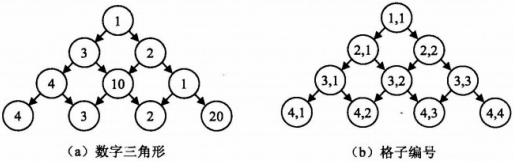
\includegraphics[width=360pt]{numbers-triangle.png}\\
\figcaption{数字三角形问题}\label{fig:numbersTriangle}
\end{center}

从第一行的数开始,每次可以往左下或右下走一格,直到走到最下行,把沿途经过的数全部加起来。
如何走才能使得这个和最大?

\subsubsection{输入}
第一行是一个整数$N (1 \le N \leq 100)$,给出三角形的行数。接下来的N行给出数字三角形。三
角形中的数全部是整数,范围在0到100之间。

\subsubsection{输出}
输出最大的和。

\subsubsection{样例输入}
\begin{Code}
5
7
3 8 
8 1 0  
2 7 4 4 
4 5 2 6 5
\end{Code}

\subsubsection{样例输出}
\begin{Code}
30
\end{Code}

\subsubsection{分析}
这是一个动态决策问题,在每层有两种选择,左下或右下,因此一个n层的数字三角形有$2^n$条路线。

可以用回溯法,用回溯法求出所有可能的路线,就可以从中选出最优路线。但是由于有$2^n$条路线,
回溯法很慢。

本题可以用动态规划来求解(具有最有子结构和重叠子问题两个要素,后面会看到)。把当前位置(i,j)看
成一个状态,然后定义状态d[i][j]为从位置(i,j)出发时能得到的最大和(包括格子(i,j)本
身的值a[i][j])。在这个状态定义下,原问题的解是d[0][0]。

下面来看看不同状态之间是怎样转移的。从位置(i,j)出发有两种决策,如果往左走,则走到(i+1,j)后需要求
“从(i+1,j)出发后能得到的最大和”这一子问题,即d[i+1][j],类似地,往右走之后需要求d[i+1][j+1]。应该
选择d[i+1][j]和d[i+1][j+1]中较大的一个,因此可以得到如下的状态转移方程:
$$d[i][j]=a[i][j]+\max\left\{d[i+1][j], d[i+1][j+1]\right\}$$

\subsubsection{代码}
版本1,备忘录法。

\begin{Codex}[label=numbers_triangle1.c]
#include<stdio.h>
#include<string.h>

#define MAXN 100

int n, a[MAXN][MAXN], d[MAXN][MAXN];

#define max(a,b) ((a)>(b)?(a):(b))

/**
 * @brief 求从位置(i,j)出发时能得到的最大和
 * @param[in] i 行
 * @param[in] j 列
 * @return 最大和
 */
int dp(const int i, const int j) {
    if(d[i][j] >= 0) {
        return d[i][j];
    } else {
        return d[i][j] = a[i][j] + (i == n-1 ? 0 : max(dp(i+1, j+1), dp(i+1, j)));
    }
}

int main() {
    int i, j;
    memset(d, -1, sizeof(d));

    scanf("%d", &n);
    for(i = 0; i < n; i++)
      for (j = 0; j <= i; j++) scanf("%d", &a[i][j]);
    
    printf("%d\n", dp(0, 0));
    return 0;
}
\end{Codex}

版本2,自底向上。

\begin{Codex}[label=numbers_triangle2.c]
#include<stdio.h>
#include<string.h>

#define MAXN 100

int n, a[MAXN][MAXN], d[MAXN][MAXN];

#define max(a,b) ((a)>(b)?(a):(b))

/**
 * @brief 自底向上计算所有子问题的最优解
 * @return 无
 */
void dp() {
    int i, j;
    for (i = 0; i < n; ++i) {
        d[n-1][i] = a[n-1][i];
    }
    for (i = n-2; i >= 0; --i)
      for (j = 0; j <= i; ++j)
        d[i][j] = a[i][j] + max(d[i+1][j], d[i+1][j+1]);
}

int main() {
    int i, j;
    memset(d, -1, sizeof(d));

    scanf("%d", &n);
    for(i = 0; i < n; i++)
      for (j = 0; j <= i; j++) 
          scanf("%d", &a[i][j]);

    dp();
    
    printf("%d\n", d[0][0]);
    return 0;
}
\end{Codex}

\subsubsection{相关的题目}
与本题相同的题目:
\begindot
\item 
《算法竞赛入门经典》\footnote{刘汝佳,算法竞赛入门经典,清华大学出版社,2009}第159页9.1.1节
\item POJ 1163 The Triangle, \myurl{http://poj.org/problem?id=1163}
\item 百练 2760 数字三角形, \myurl{http://poj.grids.cn/practice/2760/}
\item wikioi 1220 数字三角形, \myurl{http://www.wikioi.com/problem/1220/}
\myenddot

与本题相似的题目:
\begindot
\item  None
\myenddot


\subsection{过河卒}

\subsubsection{描述}
如图,A点有一个过河卒,需要走到目标B点。卒行走规则:可以向下、或者向右。同时在棋盘上的任一点有一个对方的马(如上图的C点),该马所在的点和所有跳跃一步可达的点称为对方马的控制点。例如上图C点上的马可以控制9个点(图中的P1,P2 … P8 和 C)。卒不能通过对方马的控制点。

\begin{center}
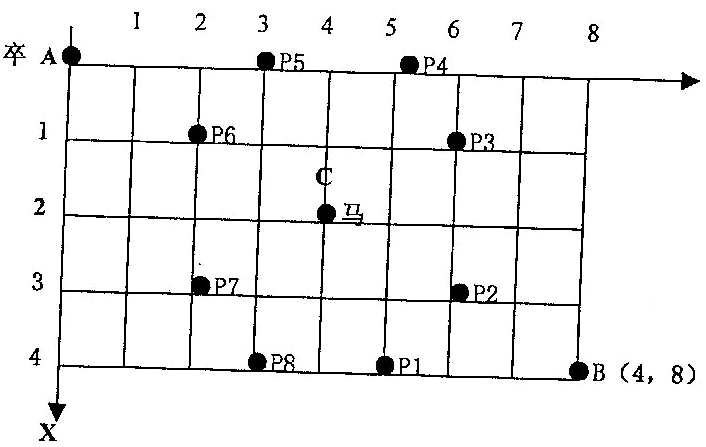
\includegraphics[width=300pt]{river.png}\\
\figcaption{过河卒}\label{fig:river}
\end{center}

棋盘用坐标表示,A点(0,0)、B点(n,m)(n,m 为不超过20的整数,并由键盘输入),同样马的位置坐标是需要给出的(约定: C不等于A,同时C不等于B)。现在要求你计算出卒从A点能够到达B点的路径的条数。

\subsubsection{输入}
B点的坐标(n,m)以及对方马的坐标(X,Y)

\subsubsection{输出}
一个整数(路径的条数)

\subsubsection{样例输入}
\begin{Code}
6 6 3 2
\end{Code}

\subsubsection{样例输出}
\begin{Code}
17
\end{Code}

\subsubsection{分析}
这是一个棋盘形动态规划。

设状态为f[i][j],表示从(0,0)到(i,j)的路径的条数,状态转移方程为
$$
f[i][j] = f[i-1][j] + f[i][j-1]
$$

\subsubsection{代码}

\begin{Codex}[label=river.c]
#include <stdio.h>
#include <memory.h>

#define MAX 21

int n, m;
int x, y; /* 马儿的坐标 */

/* 八个控制点,顺时针方向 */
int dx[] = {-2, -1, 1, 2, 2, 1, -1, -2};
int dy[] = {1, 2, 2, 1, -1, -2, -2, -1};

int g[MAX][MAX];  /* 棋盘,马儿以及马儿的控制点为1,其余为0 */
int f[MAX][MAX];  /* f[i][j] = f[i-1][j] + f[i][j-1] */

void dp() {
    int i, j;
    memset(g, 0, sizeof(g));
    memset(f, 0, sizeof(f));

    g[x][y] = 1;
    for (i = 0; i < 8; i++) if(x+dx[i] >=0 && x+dx[i] <= n &&
            y+dy[i] >= 0 && y+dy[i] <= n){
        g[x+dx[i]][y+dy[i]] = 1;
    }

    f[0][0] = 1;  /* 起点 */
    /* 初始化边界 */
    for (i = 1; i <= n; i++) if (!g[i][0]) f[i][0] = f[i-1][0];
    for (j = 1; j <= m; j++) if (!g[0][j]) f[0][j] = f[0][j-1];

    for (i = 1; i <= n; i++) {
        for (j = 1; j <= m; j++) {
            if (!g[i][j]) f[i][j] = f[i-1][j] + f[i][j-1];
        }
    }
}

int main() {
    scanf("%d%d%d%d", &n, &m, &x, &y);
    dp();
    printf("%d\n", f[n][m]);
    return 0;
}
\end{Codex}

\subsubsection{相关的题目}
与本题相同的题目:
\begindot
\item wikioi 1010, 过河卒, \myurl{http://www.wikioi.com/problem/1010/}
\myenddot

与本题相似的题目:
\begindot
\item  null
\myenddot


\subsection{传纸条}

\subsubsection{描述}
小渊和小轩是好朋友也是同班同学,他们在一起总有谈不完的话题。一次素质拓展活动中,班上同学安排做成一个$m$行$n$列的矩阵,而小渊和小轩被安排在矩阵对角线的两端,因此,他们就无法直接交谈了。幸运的是,他们可以通过传纸条来进行交流。纸条要经由许多同学传到对方手里,小渊坐在矩阵的左上角,坐标$(1,1)$,小轩坐在矩阵的右下角,坐标$(m,n)$。从小渊传到小轩的纸条只可以向下或者向右传递,从小轩传给小渊的纸条只可以向上或者向左传递。

在活动进行中,小渊希望给小轩传递一张纸条,同时希望小轩给他回复。班里每个同学都可以帮他们传递,但只会帮他们一次,也就是说如果此人在小渊递给小轩纸条的时候帮忙,那么在小轩递给小渊的时候就不会再帮忙。反之亦然。

还有一件事情需要注意,全班每个同学愿意帮忙的好感度有高有低(注意:小渊和小轩的好心程度没有定义,输入时用0表示),可以用一个$0 \sim 100$的自然数来表示,数越大表示越好心。小渊和小轩希望尽可能找好心程度高的同学来帮忙传纸条,即找到来回两条传递路径,使得这两条路径上同学的好心程度只和最大。现在,请你帮助小渊和小轩找到这样的两条路径。

\subsubsection{输入}
输入的第一行有2个用空格隔开的整数$m$和$n$,表示班里有$m$行$n$列$(1 \leq m,n \leq 50)$。接下来的$m$行是一个$m*n$的矩阵,矩阵中第$i$行$j$列的整数表示坐在第$i$行$j$列的学生的好心程度。每行的$n$个整数之间用空格隔开

\subsubsection{输出}
输出共一行,包含一个整数,表示来回两条路上参与传递纸条的学生的好心程度之和的最大值。

\subsubsection{样例输入}
\begin{Code}
3 3
0 3 9
2 8 5
5 7 0
\end{Code}

\subsubsection{样例输出}
\begin{Code}
34
\end{Code}

\subsubsection{分析}
这是一个棋盘形动态规划。用矩阵\fn{int g[MAX][MAX]}存储输入数据,即每个学生的好心值。

题目等价为为从$(1,1)$传两张纸条到$(m,n)$。每个纸条都是由上面或左边传递过来的, 所以有四种情况。设状态为$f[i][j][k][l]$,表示纸条一在$(i,j)$,纸条二在$(k,l)$的好心程度之和,状态转移方程为

\begin{eqnarray}
f[i][j][k][l] = \max\{ & f[i-1][j][k-1][l], & \nonumber \\
                            & f[i-1][j][k][l-1], & \nonumber \\
							& f[i][j-1][k][l-1], & \nonumber \\
                            & f[i][j-1][k-1][l]\} & +g[i][j]+g[k][l] \nonumber
\end{eqnarray}

\subsubsection{代码}

\begin{Codex}[label=deliver_note.c]
#include <stdio.h>
#include <memory.h>

#define MAX 51  /* m,n的最大值是50,应该有笔误,实际是51 */

int m, n;           /* 行,列 */
int g[MAX][MAX];    /* 好心值 */
/** 题目等价为为从(1,1)传两张纸条到(m,n),
 * f[i][j][k][l]表示纸条一在(i,j),纸条二在(k,l)的好心程度之和
 */
int f[MAX][MAX][MAX][MAX];

#define max(a,b) ((a)>(b)?(a):(b))

void dp() {
    int i, j, k, l;
    memset(f, 0, sizeof(f));
    /* 每个纸条都是由上面或左边传递过来的, 所以有四种情况 */
    for (i = 0; i < m; i++) {
        for (j = 0; j < n; j++) {
            for (k = 0; k < m; k++) {
                for (l = 0; l < n; l++) {
                    if(i > 0 && k > 0 && (i != k || j != l))
                        f[i][j][k][l] = max(f[i][j][k][l],
                                f[i-1][j][k-1][l] + g[i][j]+g[k][l]);
                    if(i > 0 && l < n && (i-1 != k || j != l-1))
                        f[i][j][k][l] = max(f[i][j][k][l],
                                f[i-1][j][k][l-1] + g[i][j]+g[k][l]);
                    if(j < n && l < n && (i != k || j != l))
                        f[i][j][k][l] = max(f[i][j][k][l],
                                f[i][j-1][k][l-1] + g[i][j]+g[k][l]);
                    if(j < n && k > 0 && (i != k-1 || j-1 != l))
                        f[i][j][k][l] = max(f[i][j][k][l],
                                f[i][j-1][k-1][l] + g[i][j]+g[k][l]);
                }
            }
        }
    }
}

int main() {
    int i, j;
    scanf("%d%d", &m, &n);
    for (i = 0; i < m; i++) {
        for (j = 0; j < n; j++) {
            scanf("%d", &g[i][j]);
        }
    }
    dp();
    printf("%d\n", f[m-1][n-1][m-1][n-1]);
    return 0;
}
\end{Codex}

TODO: 本题可以优化为三维

\subsubsection{相关的题目}
与本题相同的题目:
\begindot
\item wikioi 1169, 传纸条, \myurl{http://www.wikioi.com/problem/1169/}
\myenddot

与本题相似的题目:
\begindot
\item  null
\myenddot


\subsection{骑士游历}

\subsubsection{描述}
设有一个$n*m$的棋盘($2 \leq n \leq 50, 2 \leq m \leq 50$),如图~\ref{fig:horse}所示,在棋盘上有一个中国象棋马。规定:
\begindot
\item 马只能走日字
\item 马只能向右跳
\myenddot

\begin{center}
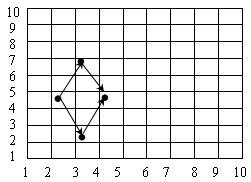
\includegraphics{horse.png} \\
\figcaption{骑士游历}\label{fig:horse}
\end{center}

问给定起点(x1,y1)和终点(x2,y2),求出马从(x1,y1)出发到(x2,y2)的合法路径条数。

\subsubsection{输入}
第一行2个整数n和m,第二行4个整数x1,y1,x2,y2

\subsubsection{输出}
合法路径条数

\subsubsection{样例输入}
\begin{Code}
30 30
1 15 3 15
\end{Code}

\subsubsection{样例输出}
\begin{Code}
2
\end{Code}

\subsubsection{分析}
这是一道棋盘型动态规划。

设状态为f[i][j],表示从起点(x1,y1)到(i,j)的合法路径条数,状态转移方程为
$$
f[i][j] = f[i-1][j-2] + f[i-1][j+2] + f[i-2][j-1] + f[i-2][j+1]
$$

注意,合法路径条数有可能非常大,32位整数存不下,需要用64位整数。

\subsubsection{代码}

\begin{Codex}[label=horse.c]
#include <stdio.h>
#include <memory.h>
#include <stdint.h>

#define MAX  51  /* n,m最大值,本题范围又有笔误,应该是51 */

int n, m;
int x1, y1, x2, y2;
/*f[i][j]表示从(x1,y1)到(i,j)的合法路径的条数*/
int64_t f[MAX+1][MAX+1];

void dp() {
    int i, j;
    memset(f, 0, sizeof(f));
    f[x1][y1] = 1;
    for (i = x1+1; i <= x2; i++) {
        for (j = 1; j <= m; j++) {
            f[i][j] = f[i-1][j-2] + f[i-1][j+2] + f[i-2][j-1] + f[i-2][j+1];
        }
    }

}

int main() {
    scanf("%d%d", &n, &m);
    scanf("%d%d%d%d", &x1, &y1, &x2, &y2);
    dp();
    printf("%lld\n", f[x2][y2]);
    return 0;
}
\end{Codex}

\subsubsection{相关的题目}
与本题相同的题目:
\begindot
\item wikioi 1219, 骑士游历, \myurl{http://www.wikioi.com/problem/1219/}
\myenddot

与本题相似的题目:
\begindot
\item  null
\myenddot


\section{划分型动态规划} %%%%%%%%%%%%%%%%%%%%%%%%%%%%%%

\subsection{乘积最大}

\subsubsection{描述}
设有一个长度为$N$的数字串,要求选手使用$K$个乘号将它分成$K+1$个部分,找出一种分法,使得这$K+1$个部分的乘积能够为最大。

举个例子:有一个数字串:312, 当$N=3$,$K=1$时会有以下两种分法:
\begindot
\item  3*12=36
\item  31*2=62
\myenddot
这时,符合题目要求的结果是:31*2=62。

\subsubsection{输入}
输入共有两行:\\
第一行共有2个自然数$N,K(6 \leq N \leq 40, 1 \leq K \leq 6)$\\
第二行是一个长度为$N$的数字串。

\subsubsection{输出}
输出最大乘积

\subsubsection{样例输入}
\begin{Code}
4 2
1231
\end{Code}

\subsubsection{样例输出}
\begin{Code}
62
\end{Code}

\subsubsection{分析}
首先,本题可以用区间型动态规划的思路解决。设状态为f[i][j][k],表示i到j这一段用k个乘号的最大乘积,状态转移方程如下:
$$
f[i][j][k] = \max\left\{f[i][s][t] * f[s+1][j][k-t-1]\right\}, i \leq s < j , 0 \leq t < k
$$

复杂度是$O(N^3K^2)$,代码如下:

\begin{Code}
/** wikioi 1017 乘积最大, http://www.wikioi.com/problem/1017 */
#include <stdio.h>
#include <stdlib.h>
#include <stdint.h>

#define MAXN 40
#define MAXK 6

int N, K;
char str[MAXN];

/** f[i][j][k]表示i到j这一段用k个乘号的最大乘积. */
int64_t f[MAXN][MAXN][MAXK+1];


#define max(a,b) ((a)>(b)?(a):(b))

/** 计算str[l,r]字符串的值,int64可以过,不用高精度. */
int64_t num(int l, int r) {
    int64_t ret = 0;
    int i;
    for (i = l; i <= r; i++) {
        ret = ret * 10 + str[i] - '0';
    }
    return ret;
}

/**
 * 区间型动态规划,复杂度是O(n^3*k^2).
 *
 * f[i][j][k] = max(f[i][s][t] * f[s+1][j][k-t-1]),
 * i <= s < j , 0 <= t < k
 */
void dp() {
    int i, j, k, s, t;
    memset(f, 0, sizeof(f));
    for (i = 0; i < N; i++) {
        for (j = i; j < N; j++) {
            f[i][j][0] = num(i, j);
        }
    }

    for (i = 0; i < N; i++) {
        for (j = i; j < N; j++) {
            for (k = 1; k <= K; k++) {
                for (s = i; s < j; s++) {
                    for (t = 0; t < k; t++) {
                        f[i][j][k] = max(f[i][j][k],
                                f[i][s][t] * f[s + 1][j][k - t - 1]);
                    }
                }
            }
        }
    }
}

int main() {
    scanf("%d%d", &N, &K);
    scanf("%s", str);
    dp();
    printf("%lld\n", f[0][N-1][K]);
    return 0;
}
\end{Code}

尽管上面的代码可以AC了,但还有更高效的思路。设状态为f[k][j],表示在区间[0,j]放入k个乘号的最大乘积,状态转移方程如下:
$$
f[k][j]=\max\left\{f[k][j], f[k-1][i]*num(i+1,j), 0 \leq i < j\right\}
$$

复杂度是$O(N^2K)$。代码如下。

\subsubsection{代码}

\begin{Codex}[label=maximal_product.c]
/** wikioi 1017 乘积最大, http://www.wikioi.com/problem/1017 */
#include <stdio.h>
#include <stdlib.h>
#include <stdint.h>

#define MAXN 40
#define MAXK 6

int N, K;
char str[MAXN];

/** f[k][j]在区间[0,j]放入k个乘号的最大乘积. */
int64_t f[MAXK+1][MAXN];


#define max(a,b) ((a)>(b)?(a):(b))

/** 计算str[l,r]字符串的值,int64可以过,不用高精度. */
int64_t num(int l, int r) {
    int64_t ret = 0;
    int i;
    for (i = l; i <= r; i++) {
        ret = ret * 10 + str[i] - '0';
    }
    return ret;
}

/** 划分型型动态规划,复杂度是O(n^3*k^2). */
void dp() {
    int i, j, k;
    memset(f, 0, sizeof(f));
    for (j = 0; j < N; j++) {
        f[0][j] = num(0, j);
    }

    for (k = 1; k <= K; k++) {
        for (j = 0; j < N; j++) {
            for (i = 0; i < j; i++) {
                f[k][j] = max(f[k][j], f[k-1][i]*num(i+1, j));
            }
        }
    }
}

int main() {
    scanf("%d%d", &N, &K);
    scanf("%s", str);
    dp();
    printf("%lld\n", f[K][N-1]);
    return 0;
}
\end{Codex}

\subsubsection{相关的题目}
与本题相同的题目:
\begindot
\item wikioi 1017, 乘积最大, \myurl{http://www.wikioi.com/problem/1017/}
\myenddot

与本题相似的题目:
\begindot
\item  null
\myenddot


\subsection{数的划分}

\subsubsection{描述}
将整数$n$分成$k$份,且每份不能为空,任意两种划分方案不能相同(不考虑顺序)。

例如:$n=7$,$k=3$,下面三种划分方案被认为是相同的。
\begin{Code}
1 1 5
1 5 1
5 1 1
\end{Code}
问有多少种不同的分法。

\subsubsection{输入}
$n,k (6<n \leq 200,2 \leq k \leq 6)$

\subsubsection{输出}
一个整数,即不同的分法。

\subsubsection{样例输入}
\begin{Code}
7 3
\end{Code}

\subsubsection{样例输出}
\begin{Code}
4
\end{Code}

\subsubsection{分析}
设状态为f[k][i],表示将整数i分成k份的方案数。有两种情况,一种划分中有至少一个1,另外一种划分中所有的数都大于1。对于第一种划分,去掉一个1,就变成了一个于子问题f[n-1][k-1],对于第二种划分,把划分中的每个数都减去1,就变成了一个子问题f[k][n-k]。因此,状态转移方程如下:
$$
f[k][i] = f[k-1][i-1] + f[k][i-k]
$$

\subsubsection{代码}

\begin{Codex}[label=integer_partition.c]
/** wikioi 1039 数的划分, http://www.wikioi.com/problem/1039 */
#include <stdio.h>
#include <memory.h>

#define MAXN 300
#define MAXK 10

int N, K;

/** f[k][i]表示将整数i分成k份的方案数. */
int f[MAXK+1][MAXN+1];

/** 划分型动态规划,复杂度是O(K*N). */
void dp() {
    int i, k;
    memset(f, 0, sizeof(f));
    for (i = 1; i <= N; i++) {
        f[1][i] = 1;
        if (i <= K) f[i][i] = 1;
    }

    for (k = 2; k <= K; k++) {
        for (i = k+1; i <= N; i++) {
            f[k][i] = f[k-1][i-1] + f[k][i-k];
        }
    }
}

int main() {
    scanf("%d%d", &N, &K);
    dp();
    printf("%d\n", f[K][N]);
    return 0;
}
\end{Codex}

\subsubsection{相关的题目}
与本题相同的题目:
\begindot
\item wikioi 1039, 数的划分, \myurl{http://www.wikioi.com/problem/1039/}
\myenddot

与本题相似的题目:
\begindot
\item  None
\myenddot


\section{树型动态规划} %%%%%%%%%%%%%%%%%%%%%%%%%%%%%%

\subsection{访问艺术馆}

\subsubsection{描述}
皮尔是一个出了名的盗画者,他经过数月的精心准备,打算到艺术馆盗画。艺术馆的结构,每条走廊要么分叉为二条走廊,要么通向一个展览室。皮尔知道每个展室里藏画的数量,并且他精确地测量了通过每条走廊的时间,由于经验老道,他拿下一副画需要5秒的时间。你的任务是设计一个程序,计算在警察赶来之前(警察到达时皮尔回到了入口也算),他最多能偷到多少幅画。

\begin{center}
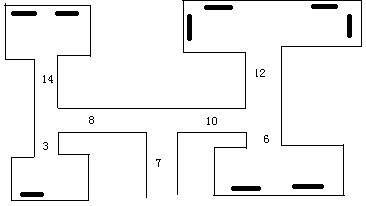
\includegraphics{gallery.png}\\
\figcaption{艺术馆}\label{fig:gallery}
\end{center}

\subsubsection{输入}
第1行是警察赶到得时间s($s \leq 600$),以秒为单位。第2行描述了艺术馆得结构,是一串非负整数,成对地出现:每一对得第一个数是走过一条走廊得时间,第2个数是它末端得藏画数量;如果第2个数是0,那么说明这条走廊分叉为两条另外得走廊。走廊的数目$ \leq 100$。数据按照深度优先得次序给出,请看样例

\subsubsection{输出}
输出偷到得画得数量

\subsubsection{样例输入}
\begin{Code}
60
7 0 8 0 3 1 14 2 10 0 12 4 6 2
\end{Code}

\subsubsection{样例输出}
\begin{Code}
2
\end{Code}

\subsubsection{分析}
设状态为f[root][time],表示在root节点,剩下time时间内能偷到的画数,则状态转移方程如下:
$$
f[root][time]=\max\left\{f[left][t]+f[right][ct-t], ct=time-T[root],0 \leq t \leq ct\right\}
$$

\subsubsection{代码}

\begin{Codex}[label=art_gallery.c]
/* wikioi 1163 访问艺术馆, http://www.wikioi.com/problem/1163/ */
#include<stdio.h>
#include <memory.h>

#define max(a,b) ((a)>(b)?(a):(b))
#define MAXN  1010  /* 走廊的最大数目 */

/* 输入数据,警察到达时间,走廊时间,藏画数量 */
int LIMIT, T[MAXN], P[MAXN];
/* 二叉树,节点个数,左孩子,右孩子 */
int n, L[MAXN], R[MAXN]; /* 0位置未用 */

/* f[root][time]表示在root节点,剩下time时间内能偷到的画数 */
int f[MAXN][MAXN];

/**
 * @brief 输入的数据是前序遍历序列,依次读入,递归建树
 * @return 根节点
 */
int build_tree() {
    n++;
    scanf("%d%d", &T[n], &P[n]);
    T[n] *= 2; /* 走廊花费时间要*2, 因为还要出来 */
    int now = n; /* 当前节点 */
    if (P[now] == 0) {
        L[now] = build_tree();  /* 建立节点now的左子树 */
        R[now] = build_tree();  /* 建立节点now的右子树 */
    }
    return now;
}

/**
 * 备忘录法.
 * @param[in] root 开始节点
 * @param[in] 剩余时间
 * @return 偷到得画的数量
 */
int dp(int root, int time) {
    int t;
    if (f[root][time] != -1)
        return f[root][time];
    if (!time)
        return f[root][time] = 0;

    const int ct = time - T[root]; /* 留给左右子节点的时间 */

    /* 到达叶子节点,即展览室 */
    if (!L[root] && !R[root]) {
        /* 不能tt / 5,因为时间够,但是可能画不够 */
        if (P[root] * 5 <= ct)
            return f[root][time] = P[root];
        else
            return f[root][time] = ct / 5;
    }

    f[root][time] = 0;
    for (t = 0; t <= ct; t++) {
        int lp = dp(L[root], t);
        int rp = dp(R[root], ct - t);
        f[root][time] = max(f[root][time], lp + rp);
    }
    return f[root][time];
}

int main() {
    scanf("%d", &LIMIT);
    build_tree();
    memset(f, -1, sizeof(f));
    printf("%d\n", dp(1, LIMIT));
    return 0;
}
\end{Codex}

\subsubsection{相关的题目}
与本题相同的题目:
\begindot
\item wikioi 1163, 访问艺术馆, \myurl{http://www.wikioi.com/problem/1163/}
\myenddot

与本题相似的题目:
\begindot
\item  None
\myenddot


\subsection{没有上司的舞会}

\subsubsection{描述}
Ural大学有$N$个职员,编号为$1 \sim N$。他们有从属关系,也就是说他们的关系就像一棵以校长为根的树,父结点就是子结点的直接上司。每个职员有一个快乐指数。现在有个周年庆宴会,要求与会职员的快乐指数最大。但是,没有职员愿和直接上司一起与会。

\subsubsection{输入}
第一行一个整数$N(1 \leq N \leq 6000)$。

接下来$N$行,第$i+1$行表示$i$号职员的快乐指数$R_i(-128 \leq R_i \leq 127)$。

接下来$N-1$行,每行输入一对整数$L,K$。表示$K$是$L$的直接上司。

最后一行输入0,0,表示结束。

\subsubsection{输出}
输出最大的快乐指数

\subsubsection{样例输入}
\begin{Code}
7
1
1
1
1
1
1
1
1 3
2 3
6 4
7 4
4 5
3 5
0 0
\end{Code}

\subsubsection{样例输出}
\begin{Code}
5
\end{Code}

\subsubsection{分析}
设状态为f[k][0]和f[k][1],f[k][0]表示第i个人不参加时的最大值,f[k][1]表示第k个人参加的最大值,则状态转移方程如下:
\begin{eqnarray}
f[k][0] &=& \sum_l\max\left\{f[l][0],f[l][1]\right\}, \text{ 其中k是l的直接上司} \nonumber \\
f[k][1] &=& \sum_l {f[l][0]}+r[k] \nonumber
\end{eqnarray}

\subsubsection{代码}

\begin{Codex}[label=ball.c]
/* wikioi 1380 没有上司的舞会, http://www.wikioi.com/problem/1380 */
#include<stdio.h>
#include<string.h>

#define MAXN 6001 /* 0位置未用 */
#define max(a,b) ((a)>(b)?(a):(b))
typedef char bool;

int n;
/* 快乐指数 */
int r[MAXN];

/* 静态链表节点. */
typedef struct edge_t {
    int v;
    int prev; /* 上一条边,倒着串起来 */
} edge_t;

/* 多个静态链表在一个数组里,实质上是树的孩子表示法 */
edge_t edge[MAXN-1];

/* head[root]指向表头,即最后一条边 */
int head[MAXN];

/* has_boss[i] 表示第i个人是否有上司 */
bool has_boss[MAXN];

int f[MAXN][2];

int cnt;  /* 边个数-1 */
void add_edge(int u, int v) {
    edge[cnt].v = v;
    edge[cnt].prev = head[u];
    head[u] = cnt++;
}

void dp(int k) {
    int p;
    f[k][1] = r[k];
    f[k][0] = 0;
    for (p = head[k]; p != -1; p = edge[p].prev) {
        int l = edge[p].v;
        dp(l);
        f[k][1] += f[l][0];
        f[k][0] = f[k][0] + max(f[l][1],f[l][0]);
    }
}

int solve() {
    int k;
    memset(f, 0, sizeof(f));
    for (k = 1; k <= n; k++) if (!has_boss[k]) {
        break;
    }

    dp(k);
    return max(f[k][0], f[k][1]);
}

int main() {
    int i;
    scanf("%d", &n);
    for (i = 1; i <= n; i++) scanf("%d", &r[i]);

    cnt = 0;
    memset(has_boss, 0, sizeof(has_boss));
    memset(head, -1, sizeof(head));
    int x, y;
    for (i = 1; i < n; i++) {
        scanf("%d%d", &x, &y);
        has_boss[x] = 1;
        add_edge(y, x);
    }
    scanf("%d%d", &x, &y);

    printf("%d\n", solve());
    return 0;
}
\end{Codex}

\subsubsection{相关的题目}
与本题相同的题目:
\begindot
\item wikioi 1380, 没有上司的舞会, \myurl{http://www.wikioi.com/problem/1380/}
\myenddot

与本题相似的题目:
\begindot
\item  None
\myenddot


\section{最大子矩形} %%%%%%%%%%%%%%%%%%%%%%%%%%%%%%
在一个给定的矩形网格中有一些障碍点,要找出网格内部不包含任何障碍点,且边界与坐标轴平行的最大子矩形。

遇到求矩形面积,一般把左上角设置为坐标原点,这与数学中的坐标系不同。

解决方法参考“浅谈用极大化思想解决最大子矩形问题”,\myurl{http://wenku.baidu.com/view/728cd5126edb6f1aff001fbb.html}

方法一是一种暴力枚举法,方法二是一种动规法。

\subsection{奶牛浴场}
\subsubsection{描述}
由于john建造了牛场围栏,激起了奶牛的愤怒,奶牛的产奶量急剧减少。为了讨好奶牛,john决定在牛场中建造一个大型浴场。但是john的奶牛有一个奇怪的习惯,每头奶牛都必须在牛场中的一个固定的位置产奶,而奶牛显然不能在浴场中产奶,于是,john希望所建造的浴场不覆盖这些产奶点。这回,他又要求助于clevow了。你还能帮助clevow吗?

john的牛场和规划的浴场都是矩形。浴场要完全位于牛场之内,并且浴场的轮廓要与牛场的轮廓平行或者重合。浴场不能覆盖任何产奶点,但是产奶点可以位于浴场的轮廓上。

clevow当然希望浴场的面积尽可能大了,所以你的任务就是帮她计算浴场的最大面积。

\subsubsection{输入}
输入文件的第一行包含两个整数L和W($1 \leq L,W \leq 30000$),分别表示牛场的长和宽。文件的第二行包含一个整数n($0 \leq n \leq 5000$),表示产奶点的数量。以下n行每行包含两个整数x和y,表示一个产奶点的坐标。所有产奶点都位于牛场内,即:$0 \leq x \leq l, 0< \leq y \leq w$。

\subsubsection{输出}
输出文件仅一行,包含一个整数S,表示浴场的最大面积。

\subsubsection{样例输入}
\begin{Code}
10 10
4
1 1
9 1
1 9
9 9
\end{Code}

\subsubsection{样例输出}
\begin{Code}
80
\end{Code}

\subsubsection{分析}
这里使用方法二,需要先做一定的预处理。由于第二种算法复杂度与牛场的面积有关,而题目中牛场的面积很大(30000×30000),因此需要对数据进行离散化处理。离散化后矩形的大小降为S×S,所以时间复杂度为O(S2),空间复杂度为O(S)。需要注意的是,为了保证算法能正确执行,把(0,0)和(m,n)设置为产奶点,相当于加上了一个“虚拟边界”。

\subsubsection{代码}
\begin{Codex}[label=cow_bath.c]
/**
 * OJ: https://vijos.org/p/1055
 */
#include <string.h>
#include <stdio.h>
#include <stdlib.h>

#define MAXN 5001

#define max(a,b) ((a)>(b)?(a):(b))
#define min(a,b) ((a)<(b)?(a):(b))

int L, W; /* 长,竖向x坐标,宽,横向y坐标 */
int n; /* n个产奶点 */
int x[MAXN], y[MAXN]; /* 产奶点坐标 */

int int_cmp(const void *a, const void *b) {
    const int *ia = (const int*) a;
    const int *ib = (const int*) b;
    return *ia - *ib;
}

/* 等价于复制粘贴,这里为了节约篇幅,使用include,在OJ上提交时请用复制粘贴 */
#include "binary_search.c"

/**
 * @brief 求最大子矩形
 *
 * 参考 http://wenku.baidu.com/view/728cd5126edb6f1aff001fbb.html 的第二种方法
 *
 * @param[in] L 长度,纵向
 * @param[in] W 宽度,横向
 * @param[in] x 纵向x坐标
 * @param[in] y 横向y坐标
 * @param[in] n 障碍点的个数
 * @return 最大子矩形的面积
 */
int max_submatrix(const int L, const int W,
        const int x[], const int y[], int n) {
    int *a = (int*) malloc((n + 1) * sizeof(int));
    int *b = (int*) malloc((n + 1) * sizeof(int));
    int la = n, lb = n;
    int i, j;
    int lm, rm; // 左边界,右边界
    int result = 0, temp;
    int **v;  // 新的01矩阵,1表示障碍点
    int *h;  // 高度
    int *l;  // 左边界
    int *r;  // 右边界

    memcpy(a, x, n * sizeof(int));
    memcpy(b, y, n * sizeof(int));
    a[la++] = 0;
    b[lb++] = 0;
    a[la++] = L;
    b[lb++] = W;

    // 去重
    qsort(a, la, sizeof(int), int_cmp);
    qsort(b, lb, sizeof(int), int_cmp);
    for (j = 1, i = 1; i < la; i++) { // 去重
        if (a[i] != a[i - 1])
            a[j++] = a[i];
    }
    la = j;
    for (j = 1, i = 1; i < lb; i++) { // 去重
        if (b[i] != b[i - 1])
            b[j++] = b[i];
    }
    lb = j;
    h = (int*) malloc(lb * sizeof(int));
    l = (int*) malloc(lb * sizeof(int));
    r = (int*) malloc(lb * sizeof(int));
    //*******************************//

    // 计算 v矩阵
    v = (int**) malloc(la * sizeof(int*));
    for (i = 0; i < la; i++) {
        v[i] = (int*) calloc(lb, sizeof(int));
    }
    for (i = 0; i < n; i++) {
        int ia, ib;
        ia = binary_search(a, la, x[i]);
        ib = binary_search(b, lb, y[i]);
        v[ia][ib] = 1; //标记障碍点
    }

    // 初始化
    for (i = 0; i < lb; i++) {
        l[i] = 0;
        r[i] = W;
        h[i] = 0;
    }

    for (i = 1; i < la; i++) { // 从上到下
        lm = 0;
        for (j = 0; j < lb; j++) { // 从左到右计算l[j]
            if (!v[i - 1][j]) {  //如果上一个不是障碍点
                h[j] = h[j] + a[i] - a[i - 1]; //高度累加
                // l[i][j]=max(l[i-1][j] , 左边第一个障碍点(i-1,j)的位置)
                l[j] = max(l[j], lm);
            } else {  //如果上一个点是障碍点
                h[j] = a[i] - a[i - 1]; //高度重新计算
                l[j] = 0;
                r[j] = W;
                lm = b[j]; //更新(i-1,j)左边第一个障碍点的位置
            }
        }
        rm = W;
        for (j = lb - 1; j >= 0; j--) {  //  从右到左计算r[j]
            //r[i][j]=min(r[i-1][j] , (i-1,j)右边第一个障碍点的位置)
            r[j] = min(r[j], rm);
            temp = h[j] * (r[j] - l[j]);
            result = max(result, temp);  //计算最优解
            if (v[i - 1][j]) //如果该点是障碍点,更新(i-1,j)右边第一个障碍点的位置
                rm = b[j];
        }
    }
    // 计算横条的面积
    for (i = 1; i < la; i++) {
        temp = W * (a[i] - a[i - 1]);
        result = max(result, temp);
    }

    free(a);
    free(b);
    for (i = 0; i < la; i++) {
        free(v[i]);
    }
    free(v);
    free(h);
    free(l);
    free(r);
    return result;
}

int main() {
    int i;
    while (scanf("%d%d", &L, &W) == 2) {
        scanf("%d", &n);
        for (i = 0; i < n; i++) {
            scanf("%d%d", &x[i], &y[i]);
        }

        printf("%d\n", max_submatrix(L, W, x, y, n));
    }
    return 0;
}
\end{Codex}

\subsubsection{相关的题目}
与本题相同的题目:
\begindot
\item Vijos 1055 奶牛浴场, \myurl{https://vijos.org/p/1055}
\myenddot

与本题相似的题目:
\begindot
\item LeetCode Maximal Rectangle, \myurl{http://leetcode.com/onlinejudge\#question_85},\\ 参考代码\myurl{https://gist.github.com/soulmachine/b20a15009450016038d9}
\item POJ 3494 Largest Submatrix of All 1's, \myurl{http://poj.org/problem?id=3494}
\myenddot


\subsection{最大全1子矩阵}
\subsubsection{描述}
给定一个$m \times n$的01矩阵,求最大的全1子矩阵。

\subsubsection{输入}
输入包含多组测试用例。每组测试用例第一行包含两个整数m和n($1 \leq m,n \leq 2000$),接下来是m行数据,每行n个元素。

\subsubsection{输出}
对每个测试用例,输出最大全1子矩阵的1的个数。如果输入的矩阵是全0,则输出0.

\subsubsection{样例输入}
\begin{Code}
2 2
0 0
0 0
4 4
0 0 0 0
0 1 1 0
0 1 1 0
0 0 0 0
\end{Code}

\subsubsection{样例输出}
\begin{Code}
0
4
\end{Code}

\subsubsection{分析}
注意,上一题算的是面积,这一题算的是个数,在某些细节上处理不同。

\subsubsection{代码}
\begin{Codex}[label=largest_rectangle.c]
#include <stdio.h>
#include <string.h>
#include <stdlib.h>

#define max(a,b)  (a > b ? a : b)
#define min(a,b)  (a < b ? a : b)

#define  MAXN 2001

int matrix[MAXN][MAXN];

int lagest_rectangle(/*int **matrix, */int m, int n) {
    int i, j;
    int *H = (int*) malloc(n * sizeof(int));  // 高度
    int *L = (int*) malloc(n * sizeof(int));  // 左边界
    int *R = (int*) malloc(n * sizeof(int));  // 右边界
    int ret = 0;

    memset(H, 0, n * sizeof(int));
    memset(L, 0, n * sizeof(int));
    for (i = 0; i < n; i++) R[i] = n;

    for (i = 0; i < m; ++i) {
        int left = 0, right = n;
        // calculate L(i, j) from left to right
        for (j = 0; j < n; ++j) {
            if (matrix[i][j] == 1) {
                ++H[j];
                L[j] = max(L[j], left);
            } else {
                left = j + 1;
                H[j] = 0;
                L[j] = 0;
                R[j] = n;
            }
        }
        // calculate R(i, j) from right to left
        for (j = n - 1; j >= 0; --j) {
            if (matrix[i][j] == 1) {
                R[j] = min(R[j], right);
                ret = max(ret, H[j] * (R[j] - L[j]));
            } else {
                right = j;
            }
        }
    }

    return ret;
}

int main() {
    int m, n;
    int i, j;
    while (scanf("%d%d", &m, &n) > 0) {
        for (i = 0; i < m; i++) {
            for (j = 0; j < n; j++) {
                scanf("%d", &matrix[i][j]);
            }
        }

        printf("%d\n", lagest_rectangle(m, n));
    }
    return 0;
}
\end{Codex}

\subsubsection{相关的题目}
与本题相同的题目:
\begindot
\item POJ 3494 Largest Submatrix of All 1's, \myurl{http://poj.org/problem?id=3494}
\item LeetCode Maximal Rectangle, \myurl{http://leetcode.com/onlinejudge\#question_85},\\ 参考代码\myurl{https://gist.github.com/soulmachine/b20a15009450016038d9}
\myenddot

与本题相似的题目:
\begindot
\item Vijos 1055 奶牛浴场, \myurl{https://vijos.org/p/1055}
\myenddot


\chapter{图}
稠密图适合用邻接矩阵来表示。
\begin{Codex}[label=am_graph.cpp]
/** 顶点数最大值. */
const int MAX_NV = 100;

/** 边的权值类型,可以为int, float, double. */
typedef int graph_weight_t;
const graph_weight_t GRAPH_INF = INT_MAX;

/**
 * @struct 图,用邻接矩阵(Adjacency Matrix).
 */
struct graph_t {
    int nv; // 顶点数
    int ne; // 边数
    // 邻接矩阵,存放边的信息,如权重等
    graph_weight_t matrix[MAX_NV][MAX_NV];
};
\end{Codex}

稀疏图适合用邻接表来表示。
\begin{Codex}[label=al_graph.cpp]
/** 边的权值类型,可以为int, float, double. */
typedef int graph_weight_t;

/** 顶点的编号,可以为char, int, string等. */
typedef char graph_vertex_id_t;

/**
 * @struct 图,用邻接表(Adjacency List).
 */
struct graph_t {
    int nv; // 顶点数
    int ne; // 边数
    // 邻接表,存放边的信息,如权重等
    map<graph_vertex_id_t, map<graph_vertex_id_t, graph_weight_t> > matrix;
};
\end{Codex}


\section{图的深搜} %%%%%%%%%%%%%%%%%%%%%%%%%%%%%%

图的深度优先搜索的代码框架如下:

\begin{Codex}[label=graph_dfs.cpp]
/**
 * @brief 图的深度优先搜索代码框架,搜索边.
 * @param[in] g 图
 * @param[in] u 出发顶点
 * @param[in] visited 边的访问历史记录
 * @return 无
 * @remark 在使用的时候,为了降低递归的内存占用量,可以把
 * g, visited 抽出来作为全局变量
 */
void dfs(const graph_t &g, int u, bool visited[][MAX_NV]) {
    for(int v = 0;  v < g.nv; v++) if(g.matrix[u][v] && !visited[u][v]) {
        visited[u][v] = visited[v][u] = true; // 无向图用这句
        // visited_edges[u][v] = true; // 有向图用这句
        dfs(g, v, visited);
        // 这里写逻辑代码
        // printf("%d %d\n", u, v);
    }
}

/**
 * @brief 图的深度优先搜索代码框架,搜索顶点.
 * @param[in] g 图
 * @param[in] u 出发顶点
 * @param[in] visited 顶点的访问历史记录
 * @return 无
 * @remark 在使用的时候,为了降低递归的内存占用量,可以把
 * g, visited 抽出来作为全局变量
 */
void dfs(const graph_t &g, int u, bool visited[MAX_NV]) {
    visited[u] = true;
    for(int v = 0;  v < g.nv; v++) if(g.matrix[u][v] && !visited[v]) {
        dfs(g, v, visited);
        // 这里写逻辑代码
        // printf("%d %d\n", u, v);
    }
}
\end{Codex}


\subsection{Satellite Photographs}

\subsubsection{描述}
Farmer John purchased satellite photos of $W \times H$ pixels of his farm ($1 \leq W \leq 80, 1 \leq H \leq 1000$) and wishes to determine the largest 'contiguous' (connected) pasture. Pastures are contiguous when any pair of pixels in a pasture can be connected by traversing adjacent vertical or horizontal pixels that are part of the pasture. (It is easy to create pastures with very strange shapes, even circles that surround other circles.) 

Each photo has been digitally enhanced to show pasture area as an asterisk ('*') and non-pasture area as a period ('.'). Here is a $10 \times 5$ sample satellite photo: 
\begin{Code}
..*.....** 
.**..***** 
.*...*.... 
..****.*** 
..****.*** 
\end{Code}

This photo shows three contiguous pastures of 4, 16, and 6 pixels. Help FJ find the largest contiguous pasture in each of his satellite photos.


\subsubsection{输入}
Line 1: Two space-separated integers: $W$ and $H$ 

Lines 2..H+1: Each line contains $W$ "*" or "." characters representing one raster line of a satellite photograph.


\subsubsection{输出}
Line 1: The size of the largest contiguous field in the satellite photo.


\subsubsection{样例输入}
\begin{Code}
10 5
..*.....**
.**..*****
.*...*....
..****.***
..****.***
\end{Code}


\subsubsection{样例输出}
\begin{Code}
16
\end{Code}


\subsubsection{分析}
这是一个平面的二维地图,把地图上的每个点当成隐式图上的一个顶点,每个顶点有上下左右四个邻接点。在这个隐式图上进行深搜。


\subsubsection{代码}
\begin{Codex}[label=satellite_photographs.c]
/* POJ 3051 Satellite Photographs, http://poj.org/problem?id=3051 */
#include <stdio.h>
#include <string.h>

#define MAXH 1000
#define MAXW 80

int H, W; /* H行W列 */
char map[MAXH+2][MAXW+2];/* 上下左右加一圈'.'可以防止越界 */

int count;

void dfs(int x, int y) {
    /* 加了一圈'.'可以防止越界,因此不需要判断越界 */
    if (map[x][y] == '.') return;

    map[x][y] = '.';  /* 标记(x,y)已访问过,起到去重作用 */
    count++;
    dfs(x + 1, y);
    dfs(x - 1, y);
    dfs(x, y + 1);
    dfs(x, y - 1);
}

int main() {
    int i, j, max;
    memset(map, '.', sizeof(map));

    scanf("%d%d", &W, &H); /* H是行数,W是列数 */
    for(i = 1; i <= H; ++i) {
        char line[MAXW+1];
        scanf("%s", line);
        strncpy(&map[i][1], line, W);
    }

    max = 0;
    for (i = 1; i <= H; i++) {
        for (j = 1; j <= W; j++) {
            if (map[i][j] == '*') {
                count = 0;
                dfs(i, j);
            }
            if (count > max) max = count;
        }
    }
    printf("%d\n", max);
    return 0;
}
\end{Codex}


\subsubsection{相关的题目}
与本题相同的题目:
\begindot
\item POJ 3051 Satellite Photographs, \myurl{http://poj.org/problem?id=3051}
\myenddot

与本题相似的题目:
\begindot
\item POJ 3620 Avoid The Lakes, \myurl{http://poj.org/problem?id=3620} \\ 参考代码 \myurl{https://gist.github.com/soulmachine/6761537}
\myenddot


\subsection{John's trip}


\subsubsection{Description}
Little Johnny has got a new car. He decided to drive around the town to visit his friends. Johnny wanted to visit all his friends, but there was many of them. In each street he had one friend. He started thinking how to make his trip as short as possible. Very soon he realized that the best way to do it was to travel through each street of town only once. Naturally, he wanted to finish his trip at the same place he started, at his parents' house. 

The streets in Johnny's town were named by integer numbers from 1 to $n, n < 1995$. The junctions were independently named by integer numbers from 1 to $m, m <= 44$. No junction connects more than 44 streets. All junctions in the town had different numbers. Each street was connecting exactly two junctions. No two streets in the town had the same number. He immediately started to plan his round trip. If there was more than one such round trip, he would have chosen the one which, when written down as a sequence of street numbers is lexicographically the smallest. But Johnny was not able to find even one such round trip. 

Help Johnny and write a program which finds the desired shortest round trip. If the round trip does not exist the program should write a message. Assume that Johnny lives at the junction ending the street appears first in the input with smaller number. All streets in the town are two way. There exists a way from each street to another street in the town. The streets in the town are very narrow and there is no possibility to turn back the car once he is in the street 


\subsubsection{Input}
Input file consists of several blocks. Each block describes one town. Each line in the block contains three integers $x; y; z$, where $x > 0$ and $y > 0$ are the numbers of junctions which are connected by the street number $z$. The end of the block is marked by the line containing $x = y = 0$. At the end of the input file there is an empty block, $x = y = 0$.


\subsubsection{Output}
Output one line of each block contains the sequence of street numbers (single members of the sequence are separated by space) describing Johnny's round trip. If the round trip cannot be found the corresponding output block contains the message "Round trip does not exist."


\subsubsection{Sample Input}
\begin{Code}
1 2 1
2 3 2
3 1 6
1 2 5
2 3 3
3 1 4
0 0
1 2 1
2 3 2
1 3 3
2 4 4
0 0
0 0
\end{Code}

\subsubsection{Sample Output}
\begin{Code}
1 2 3 5 4 6 
Round trip does not exist.
\end{Code}

\subsubsection{分析}
欧拉回路。

如果能从图的某一顶点出发,每条边恰好经过一次,这样的路线称为\textbf{欧拉道路}(Eulerian Path)。
如果还能够回到起点,这样的路线称为\textbf{欧拉回路}(Eulerian Circuit)。

对于无向图G,当且仅当G是连通的,且最多有两个奇点,则存在欧拉道路。
如果有两个奇点,则必须从其中一个奇点出发,到另一个奇点终止。

如果没有奇点,则一定存在一条欧拉回路。

对于有向图G,当且仅当G是连通的,且每个点的入度等于出度,则存在欧拉回路。

如果有两个顶点的入度与出度不相等,且一个顶点的入度比出度小1,另一个顶点的入度比出度大1,此时,
存在一条欧拉道路,以前一个顶点为起点,以后一个顶点为终点。


\subsubsection{代码}
\begin{Codex}[label=round_trip.cpp]
// POJ 1041 John's trip, http://poj.org/problem?id=1041
#include <iostream>
#include <cstring>
#include <algorithm>
#include <stack>

using namespace std;

const int MAX_NV = 45;
const int MAX_NE = 1996;

/**
 * @struct 图,邻接矩阵的变种.
 */
struct graph_t {
    int nv; // 顶点数
    int ne; // 边数
    // G[点][边] = 点,这样是为了能方便让边lexicographically输出
    int matrix[MAX_NV][MAX_NE];
};

graph_t G;

bool visited[MAX_NE];  // 边是否已访问
int degree[MAX_NV];    // 点的度

stack<int> s;  // 栈,用于输出

void stack_print(stack<int> &s) {
    while (!s.empty()) {
        cout << s.top() << " ";
        s.pop();
    }
    cout << endl;
}

void euler(int u) {
    for (int e = 1; e <= G.ne; e++) {
        if (!visited[e] && G.matrix[u][e]) { //若相邻边未访问过
            visited[e] = true;
            euler(G.matrix[u][e]);
            s.push(e);
        }
    }
}

int main() {
    int x, y, z, start;
    while ((cin >> x >> y) && x && y) {
        memset(visited, false, sizeof(visited));
        memset(degree, 0, sizeof(degree));
        memset(&G, 0, sizeof(G));

        start = x < y ? x : y;
        cin >> z;
        G.ne = max(G.ne, z);
        G.nv = max(G.nv, max(x, y));
        G.matrix[x][z] = y;
        G.matrix[y][z] = x;
        ++degree[x];
        ++degree[y];

        while ((cin >> x >> y) && x && y) {
            cin >> z;
            G.ne = max(G.ne, z);
            G.nv = max(G.nv, max(x, y));
            G.matrix[x][z] = y;
            G.matrix[y][z] = x;
            ++degree[x];
            ++degree[y];
        }

        /* 欧拉回路形成的条件之一,判断结点的度是否为偶数 */
        bool flag = true;
        for (int i = 1; i <= G.nv; i++) {
            if (degree[i] & 1) {
                flag = false;
                break;
            }
        }

        if (!flag) {
            cout << "Round trip does not exist." << endl;
        } else {
            euler(start);
            stack_print(s);
        }
    }
    return 0;
}
\end{Codex}


\subsubsection{相关的题目}
与本题相同的题目:
\begindot
\item POJ 1041 John's trip, \myurl{http://poj.org/problem?id=1041}
\myenddot

与本题相似的题目:
\begindot
\item 《算法竞赛入门经典》\footnote{刘汝佳,算法竞赛入门经典,清华大学出版社,2009} 第111页6.4.4节
\item  UVa 10054 The Necklace, \myurl{http://t.cn/zRwqcRp}
\item  UVa 10129 Play on Words, \myurl{http://t.cn/zTInBDX}
\myenddot


\subsection{The Necklace}

\subsubsection{描述}
My little sister had a beautiful necklace made of colorful beads. Two successive beads in the 
necklace shared a common color at their meeting point. The figure below shows a segment of 
the necklace:
 
\centerline{\fbox{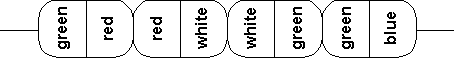
\includegraphics[width=240pt]{uva10054.png}}}
 
But, alas! One day, the necklace was torn and the beads were all scattered over the floor. 
My sister did her best to recollect all the beads from the floor, but she is not sure 
whether she was able to collect all of them. Now, she has come to me for help. She wants
 to know whether it is possible to make a necklace using all the beads she has in the same
 way her original necklace was made and if so in which order the bids must be put.
 
Please help me write a program to solve the problem.
 
\subsubsection{Input}
The input contains T test cases. The first line of the input contains the integer T.
 
The first line of each test case contains an integer $N(5 \leq N \leq 1000)$ giving the number of beads 
my sister was able to collect. Each of the next N lines contains two integers describing 
the colors of a bead. Colors are represented by integers ranging from 1 to 50.
 
\subsubsection{Output}
For each test case in the input first output the test case number as shown in the sample output. Then 
if you apprehend that some beads may be lost just print the sentence ``some beads may be lost" on a 
line by itself. Otherwise, print N lines with a single bead description on each line. Each bead 
description consists of two integers giving the colors of its two ends. For $1 \leq i \leq N_1$, the second integer 
on line i must be the same as the first integer on line i + 1. Additionally, the second integer 
on line N must be equal to the first integer on line 1. Since there are many solutions, any one
 of them is acceptable.
 
Print a blank line between two successive test cases.
 
\subsubsection{Sample Input}
\begin{Code}
2
5
1 2
2 3
3 4
4 5
5 6
5
2 1
2 2
3 4
3 1
2 4
\end{Code}
 
\subsubsection{Sample Output}
\begin{Code}
Case #1
some beads may be lost
 
Case #2
2 1
1 3
3 4
4 2
2 2
\end{Code}
 
\subsubsection{分析}
欧拉回路。
 
注意顶点可以有自环。


\subsubsection{代码}
\begin{Codex}[label=eulerian_circuit.c]
#include <stdio.h>
#include<string.h>
 
#define MAXN 51  // 顶点最大个数
 
int G[MAXN][MAXN];
int visited_vertices[MAXN]; 
int visited_edges[MAXN][MAXN];
int count[MAXN]; // 顶点的度
 
void dfs(const int u) {  
    int v;
    visited_vertices[u] = 1;
    for(v = 0;  v < MAXN; v++) if(G[u][v] && !visited_vertices[v]) {
        dfs(v);
    }
}
 
/*
 * @brief 欧拉回路,允许自环和重复边
 * @param[in] u 起点
 * @return 无
 */
void euler(const int u){
    int v;
    for(v = 0; v < MAXN; ++v) if(G[u][v]){
        --G[u][v]; --G[v][u]; // 这个技巧,即有visited的功能,又允许重复边
        euler(v);
        // 逆向打印,或者存到栈里再打印
        printf("%d %d\n", u, v);
    }
}
 
int main() {
    int T, N, a, b;
    int i;
    int cases=1;
    scanf("%d",&T);
    while(T--) {
        int flag = 1; // 结点的度是否为偶数
        int flag2 = 1; // 图是否是连通的
        
        memset(G, 0, sizeof(G));
        memset(count, 0, sizeof(count));
 
        scanf("%d",&N);
        for(i = 0; i < N; ++i){
            scanf("%d %d", &a, &b); 
            ++G[a][b];
            ++G[b][a];
            ++count[a];
            ++count[b];
        }
 
        printf("Case #%d\n", cases++);
 
        // 欧拉回路形成的条件之一,判断结点的度是否为偶数
        for(i=0; i<MAXN; ++i) {
            if(count[i] & 1){
                flag = 0;
                break;
            }
        }
        // 检查图是否连通
        if(flag) {
            memset(visited_vertices, 0, sizeof(visited_vertices));
            memset(visited_edges, 0, sizeof(visited_edges));
 
            for(i=0; i< MAXN; ++i) 
                if(count[i]) { 
                    dfs(i);
                    break; 
                }
            for(i=0; i< MAXN; ++i){
                if(count[i] && !visited_vertices[i]) {
                    flag2 = 0; 
                    break;
                }
            }
        }
        if (flag && flag2) {
            for(i = 0; i < MAXN; ++i) if(count[i]){
                euler(i);
                break;
            }
        } else {
            printf("some beads may be lost\n");
        }
 
        if(T > 0) printf("\n");
    }
    return 0;
}
\end{Codex}


\subsubsection{相关的题目}

与本题相同的题目:
\begindot
\item  UVa 10054 The Necklace, \myurl{http://t.cn/zRwqcRp}
\myenddot

与本题相似的题目:
\begindot
\item 《算法竞赛入门经典》\footnote{刘汝佳,算法竞赛入门经典,清华大学出版社,2009} 第111页6.4.4节
\item POJ 1041 John's trip, \myurl{http://poj.org/problem?id=1041}
\item UVa 10129 Play on Words, \myurl{http://t.cn/zTInBDX}
\myenddot


\section{图的广搜} %%%%%%%%%%%%%%%%%%%%%%%%%%%%%%



\section{最小生成树} %%%%%%%%%%%%%%%%%%%%%%%%%%%%%%
“最小”指的是边的权值之和最小。

构造最小生成树(Minimum Spanning Tree, MST)有多种算法。其中多数算法利用了最小生成树的一个性质(简称为MST性质):假设$N=(V, E)$是一个连通网,$U$是顶点集$V$的一个非空子集。若$(u, v)$是一条具有最小权值的边,其中$u \in U, v \in V-U$,则必存在一颗包含边$(u, v)$的最小生成树。

Prim算法和Kruskal算法是两个利用MST性质构造最小生成树的算法。它们都属于贪心法。

\subsection{Prim算法}
假设$N=(V, E)$是一个连通网,$TE$是$N$上最小生成树中边的集合。算法从$U={u_0}(u_0 \in V), TE=\{\}$开始,重复执行下述操作:在所有$u \in U, v \in V-U$的边$(u, v) \in E$中找一条代价最小的边$(u_0, v_0)$并入集合$TE$,同时$v_0$并入U,直至$U=V$为止。此时$TE$中必有$n-1$条边,则$T=(V, TE)$为$N$的最小生成树。
为实现这个算法需附设一个数组\fn{closedge},以记录从$U$到$V-U$具有最小代价的边。对每个顶点$v_i \in V-U$,在辅助数组中存在一个相应分量\fn{closedge[i-1]},它包括两个域,其中\fn{lowcost}存储该边上的权。显然,$closedge[i].lowcost=\min\left\{cost(u, v_i), u \in U\right\}$。\fn{adjvex}域存储该边依附的在U中的顶点。

图 \ref{fig:prim}所示为按Prim算法构造网的一棵最小生成树的过程,在构造过程中辅助数组中各分量值的变化如表\ref{tab:prim}所示。

\begin{center}
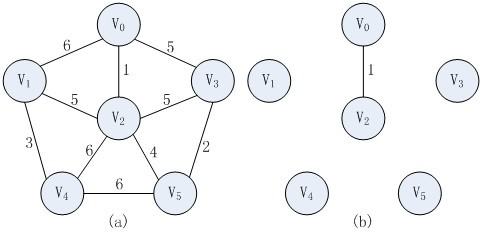
\includegraphics[width=240pt]{prim1.png}\\
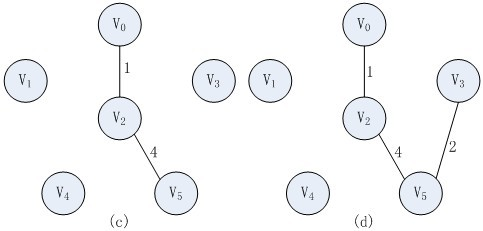
\includegraphics[width=240pt]{prim2.png}\\
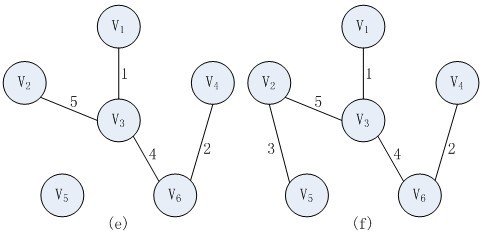
\includegraphics[width=240pt]{prim3.png}\\
\figcaption{Prim算法构造最小生成树的过程}\label{fig:prim}
\end{center}

\begin{center}
\tabcaption{构造最小生成树过程中辅助数组的变化}
\label{tab:prim}
\begin{tabular}{|c|cccccccc|}
\hline
\textbf{\diagbox{closedge}{i}} & \textbf{1} & \textbf{2} & \textbf{3} & \textbf{4}& \textbf{5}& \textbf{U}& \textbf{U-V}& \textbf{k}\\
\hline
adjvex & $v_0$ & $v_0$ & $v_0$ & & & $v_0$ & $\{v_1,v_2,v_3,v_4,v_5\}$ & \multirow{2}{*}{2} \\
lowcost & 6 & 1 & 5 & & & & & \\
\hline
adjvex & $v_2$ & & $v_1$ & $v_2$ & $v_2$ & $\{v_0,v_2\}$ & $\{v_1,v_3,v_4,v_5\}$ & \multirow{2}{*}{5} \\
lowcost & 5 & 0 & 5 & 6 & 4 & & & \\
\hline
adjvex & $v_2$ & & $v_6$ & $v_2$ & & $\{v_0,v_2,v_5\}$ & $\{v_1,v_3,v_4\}$ & \multirow{2}{*}{3} \\
lowcost & 5 & 0 & 2 & 6 & 0 & & & \\
\hline
adjvex & $v_2$ & & & $v_2$ & & $\{v_0,v_2,v_5,v_3\}$ & $\{v_1,v_4\}$ & \multirow{2}{*}{1} \\
lowcost & 5 & 0 & 0 & 6 & 0 & & & \\
\hline
adjvex & & & & $v_1$ & & $\{v_0,v_2,v_5,v_3,v_1\}$ & $\{v_4\}$ & \multirow{2}{*}{4} \\
lowcost & 0 & 0 & 0 & 3 & 0 & & & \\
\hline
adjvex & & & & & & $\{v_0,v_2,v_5,v_3,v_1,v_4\}$ & $\{\}$ & \multirow{2}{*}{} \\
lowcost & 0 & 0 & 0 & 0 & 0 & & & \\
\hline
\end{tabular}
\end{center}


\subsubsection{代码}

\begin{Codex}[label=am_graph_prim1.cpp]
#include <iostream>
#include <climits>  /* for INT_MAX */

using namespace std;

/** 顶点数最大值. */
const int MAX_NV = 100;

/** 边的权值类型,可以为int, float, double. */
typedef int graph_weight_t;
const graph_weight_t GRAPH_INF = INT_MAX;

/**
 * @struct 图,用邻接矩阵(Adjacency Matrix).
 */
struct graph_t {
    int nv; // 顶点数
    int ne; // 边数
    // 邻接矩阵,存放边的信息,如权重等
    graph_weight_t matrix[MAX_NV][MAX_NV];
};

graph_t g;

struct closedge_t {
    int adjvex; /* 弧头,属于U */
    /* 边 adjvex->本下标 的权值,-GRAPH_INF表示已经加入U */
    graph_weight_t lowcost;
};

/*
 * @brief 在V-E集合中寻找最小的边
 * @param[in] closedge MST中的边,起点为adjvex,终点为本下标
 * @param[in] n closedge数组的长度
 * @return 找到了则返回弧尾的下标,V-U为空集则返回-1,表示终止
 */
static int min_element(const closedge_t closedge[], int n) {
    int min_value = GRAPH_INF;
    int min_pos = -1;
    for (int i = 0; i < n; i++)
        if (closedge[i].lowcost > -GRAPH_INF) {
            if (min_value > closedge[i].lowcost) {
                min_value = closedge[i].lowcost;
                min_pos = i;
            }
        }
    return min_pos;
}

/**
 * @brief Prim算法,求图的最小生成树.
 * @param[in] g 图对象的指针
 * @return MST的边的权值之和
 */
graph_weight_t prim(const graph_t &g) {
    graph_weight_t sum = 0; /* 权值之和 */
    int u = 0; /* 从0号顶点出发 */
    const int n = g.nv;
    /* closedge[n],记录从顶点集U到V-U的边*/
    closedge_t* const closedge = new closedge_t[n];

    /* 辅助数组初始化*/
    for (int i = 0; i < n; i++) if (i != u) {
        closedge[i].adjvex = u;
        closedge[i].lowcost = g.matrix[u][i];
    }
    closedge[u].lowcost = -GRAPH_INF; /* 初始, U={u} */

    for (int i = 0; i < n; i++) if (i != u) { /* 其余的n-1个顶点*/
        /* 求出TE的下一个顶点k */
        const int k = min_element(closedge, n);
        /* 输出此边 closedge[k].adjvex --> k */
        cout << (char)('A' + closedge[k].adjvex) << " - " << (char)('A' + k)
                << " : "<< g.matrix[closedge[k].adjvex][k] << endl;
        sum += g.matrix[closedge[k].adjvex][k];
        // sum += closedge[k].lowcost;  // 等价
        closedge[k].lowcost = -GRAPH_INF;  /* 顶点k并入U,表示此边加入TE */
        /* 更新k的邻接点的值,不相邻为无穷大*/
        for (int j = 0; j < n; j++) {
            const graph_weight_t w = g.matrix[k][j];
            if (w < closedge[j].lowcost) {
                closedge[j].adjvex = k;
                closedge[j].lowcost = w;
            }
        }
    }
    delete[] closedge;
    return sum;
}

/** 读取输入,构建图. */
void read_graph() {
    int m, n;

    /* 读取节点和边的数目 */
    cin >> m >> n;
    g.nv = m;
    g.ne = n;

    /* 初始化图,所有节点间距离为无穷大 */
    for (int i = 0; i < m; i++) {
        for (int j = 0; j < m; j++) {
            g.matrix[i][j] = GRAPH_INF;
        }
    }

    /* 读取边信息 */
    for (int k = 0; k < n; k++) {
        char chx, chy;
        int w;
        cin >> chx >> chy >> w;
        const int i = chx - 'A';
        const int j = chy - 'A';
        g.matrix[i][j] = w;
        g.matrix[j][i] = w;
    }
}

/* test
输入数据:
7 11
A B 7
A D 5
B C 8
B D 9
B E 7
C E 5
D E 15
D F 6
E F 8
E G 9
F G 11

输出:
A - D : 5
D - F : 6
A - B : 7
B - E : 7
E - C : 5
E - G : 9
Total:39
*/
int main() {
    read_graph();
    cout << "Total : " << prim(g) << endl;
    return 0;
}
\end{Codex}


\subsubsection{算法分析}
假设网中有$n$个顶点,则第一个进行初始化的循环语句的频度为$n$,第二个循环语句的频度为$n-1$。其中有两个内循环:其一是在\fn{closedge[v].lowcost}中求最小值,其频度为$n-1$;其二是重新选择具有最小代价的边,其频度为$n$。因此Prim算法的时间复杂度为$O(n^2)$,与网中边数无关,因此适用于求边稠密的图的最小生成树。

Prim算法的另一种实现是使用小根堆,其流程是:小根堆中存储一个端点在生成树中,另一个端点不在生成树的边,每次从小根堆的堆顶可选出权值最小的边$(u, v)$,将其从堆中推出,加入生成树中。然后将新出现的所有一个端点在生成树中,一个端点不在生成树的边都插入小根堆中。下一轮迭代中,下一条满足要求的边又上升到堆顶。如此重复$n-1$次,最后建立起该图的最小生成树。该算法的C代码实现如下。


\subsubsection{代码}

\begin{Codex}[label=am_graph_prim2.cpp]
#include <iostream>
#include <climits>  /* for INT_MAX */
#include <queue>
#include <algorithm>

using namespace std;

/** 顶点数最大值. */
const int MAX_NV = 100;

/** 边的权值类型,可以为int, float, double. */
typedef int graph_weight_t;
const graph_weight_t GRAPH_INF = INT_MAX;

/**
 * @struct 图,用邻接矩阵(Adjacency Matrix).
 */
struct graph_t {
    int nv; // 顶点数
    int ne; // 边数
    // 邻接矩阵,存放边的信息,如权重等
    graph_weight_t matrix[MAX_NV][MAX_NV];
};

graph_t g;

/**
 * @struct 边
 */
struct edge_t{
    int u;  // from
    int v;  // to
    graph_weight_t w;  // 权值

    bool operator>(const edge_t &other) const {
        return w > other.w;
    }
};

/**
  * @brief Prim算法,求图的最小生成树.
  * @param[in] g 图对象的指针
  * @return MST的边的权值之和
  */
int prim(const graph_t &g){
    graph_weight_t sum = 0; // 权值之和
    priority_queue<edge_t, vector<edge_t>, greater<edge_t> > q;
    const int n = g.nv;
    bool* used = new bool[n];  // 判断顶点是否已经加入最小生成树
    std::fill(used, used + n, false);

    int count = 1;  // MLE 当前的边数
    int u = 0;      // 从0号顶点出发
    used[u] = true;    // 开始顶点加入U(所以count初始为1)
    while (count < n) {
        for(int v = 0; v < n; v++) if(!used[v]) { // 若v不在生成树,(u,v)加入堆
            edge_t e = {u, v, g.matrix[u][v]};
            q.push(e);
        }
        while(!q.empty() && count < n) {
            const edge_t e = q.top(); q.pop();  // 从堆中退出最小权值边,存入 e
            if(!used[e.v]) {
                // 输出生成树TE的边,即此边加入TE
                cout << (char)('A' + e.u) << " - " << (char)('A' + e.v) <<
                        " : " << g.matrix[e.u][e.v] << endl;
                sum += g.matrix[e.u][e.v];
                u = e.v;
                used[u] = true; // u并入到生成树的顶点集合U
                count++;
                break;
            }
        }
    }

    delete[] used;
    return sum;
}

// ...
\end{Codex}

\subsubsection{算法分析}
该算法迭代次数为$O(n)$,每次迭代将平均$e/n$条边插入最小堆中,$e$条边从堆中删除,堆的插入和删除操作时间复杂度均为$O(\log_2 e)$,则总的时间复杂度为 $O(e\log_2e)$。

\subsection{Kruskal算法}
\label{sec:kruskal}
假设连通网$N={V, E}$,则令最小生成树的初始状态为只有$n$个顶点而无边的非连通图$T=(V, {})$,图中每个顶点自成一个连通分量。在$E$中选择代价最小的边,若该边依附的顶点落在$T$中不同的连通分量上,则将此边加入到$T$中,否则舍去此边而选择下一条代价最小的边。依次类推,直至T中所有顶点都在同一连通分量上为止。

图\ref{fig:kruskal}所示为Kruskal算法构造一棵最小生成树的过程。

\begin{center}
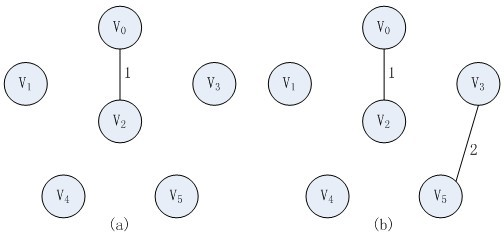
\includegraphics[width=240pt]{kruskal1.png}\\
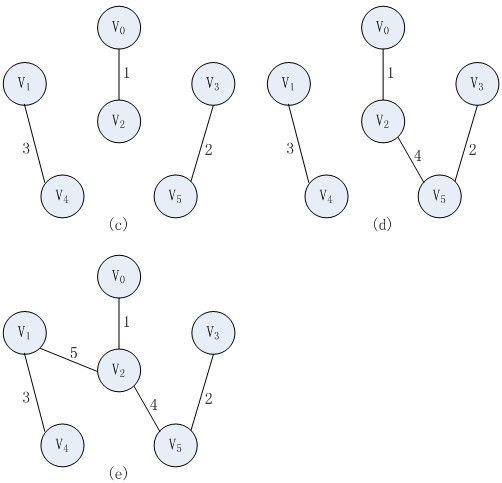
\includegraphics[width=240pt]{kruskal2.png}\\
\figcaption{Kruskal算法构造最小生成树的过程}\label{fig:kruskal}
\end{center}

下面是Kruskal算法的C语言实现。

\subsubsection{代码}

\begin{Codex}[label=kruskal.cpp]
#include <iostream>
#include <climits>  /* for INT_MAX */
#include <queue>
#include <algorithm>

using namespace std;

/* 等价于复制粘贴,这里为了节约篇幅,使用include,在OJ上提交时请用复制粘贴 */
#include "ufs.c"  /* 见“树->并查集”这节 */

const int MAX_NV = 11; /* 顶点数最大值 */
const int MAX_NE = 100;  /* 最大边数 */
/** 边的权值类型. */
typedef int graph_weight_t;

/** 图的边. */
struct edge_t{
    int u;  /** 顶点编号 */
    int v;  /** 顶点编号 */
    graph_weight_t w;  /** 权值 */

    bool operator>(const edge_t &other) const {
        return w > other.w;
    }
};

edge_t edges[MAX_NE];


/*
  * @brief Kruskal算法,堆+并查集.
  * @param[in] edges 边的数组
  * @param[in] n 边数,一定要大于或等于(顶点数-1)
  * @param[in] m 顶点数
  * @return MST的边的权值之和
  */
graph_weight_t kruskal(const edge_t edges[], int n, int m) {
    graph_weight_t sum = 0;
    priority_queue<edge_t, vector<edge_t>,
                                greater<edge_t> > q;
    ufs_t *s = ufs_create(MAX_NV);
    if (n < m - 1) return -1;

    /* 把所有边插入堆中*/
    for (int i = 0; i < n; i++) {
        q.push(edges[i]);
    }

    for (int i = 0; i < n; i++) {
        /* 从堆中退出最小权值边 */
        const edge_t e = q.top(); q.pop();
        /* 取两顶点所在集合的根*/
        const int u = ufs_find(s, e.u);
        const int v = ufs_find(s, e.v);
        if (u != v) { /* 不是同一集合,说明不连通*/
            ufs_union(s, u, v); /* 合并,连通成一个分量*/
            /* 输出生成树TE的边,即此边加入TE */
            cout << (char)('A' + e.u) << " - " << (char)('A' + e.v) << endl;
            sum += e.w;
        }
    }

    ufs_destroy(s);
    return sum;
}

bool operator<(const edge_t &e1, const edge_t &e2) {
    return e1.w < e2.w;
}

/** Kruskal算法,快排+并查集. */
graph_weight_t kruskal1(edge_t edges[], int n, int m) {
    graph_weight_t sum = 0;
    ufs_t *s = ufs_create(MAX_NV);  /* 并查集,0位置未用  */
    if (n < m - 1) return -1;

    std::sort(edges, edges + n);

    for (int i = 0; i < n; i++) {
        /* 从堆中退出最小权值边,存入ed */
        const edge_t e = edges[i];
        /* 取两顶点所在集合的根*/
        const int u = ufs_find(s, e.u);
        const int v = ufs_find(s, e.v);
        if (u != v) { /* 不是同一集合,说明不连通*/
            ufs_union(s, u, v); /* 合并,连通成一个分量*/
            /* 输出生成树TE的边,即此边加入TE */
            cout << (char)('A' + e.u) << " - " << (char)('A' + e.v) << endl;
            sum += e.w;
        }
    }
    ufs_destroy(s);
    return sum;
}

/* test
输入数据:
7 11
A B 7
A D 5
B C 8
B D 9
B E 7
C E 5
D E 15
D F 6
E F 8
E G 9
F G 11

输出:
A - D
C - E
D - F
B - E
A - B
E - G
Total : 39
*/
int main() {
    int m, n;
    /* 读取顶点数,边数目*/
    cin >> m >> n;

    /* 读取边信息 */
    for (int i = 0; i < n; i++) {
        char chx, chy;
        int w;
        cin >> chx >> chy >> w;

        edges[i].u = chx - 'A';
        edges[i].v = chy - 'A';
        edges[i].w = w;
    }

    /* 求解最小生成树 */
    cout << "Total : " << kruskal(edges, n, m) << endl;
    return 0;
}
\end{Codex}

\subsubsection{算法分析}
如果采用邻接矩阵作为图的存储结构,则在建立小根堆时需要检测图的邻接矩阵,这需要$O(n^2)$的时间。此外,需要将$e$条边组成初始的小根堆。如果直接从空堆开始,依次插入各边,需要$O(e\log_2e)$的时间。在构造最小生成树的过程中,需要进行$O(e)$次出堆操作\fn{heap_remove()}、$2e$次并查集的\fn{ufs_find()}操作以及$n-1$次\fn{ufs_union()}操作,计算时间分别为$O(e\log_2e)$、$O(\log_2n)$和$O(n)$,所以总时间为$O(n^2+e\log_2e)$。

如果采用邻接表作为图的存储结构,则在建立小根堆时需要检测图的邻接表,这需要$O(n+e)$的时间。为建成初始的小根堆,需要$O(e\log_2e)$的时间。在构造最小生成树的过程中,需要进行$O(e)$次出堆操作\fn{heap_remove()}、$2e$次并查集的\fn{ufs_find()}操作以及$n-1$次\fn{ufs_union()}操作,计算时间分别为$O(e\log_2e)$、$O(e\log_2n)$和$O(n)$,所以总时间为$O(n+e\log_2e)$。


\subsection{Highways}
\subsubsection{描述}
一个名叫Flatopia的岛国地势非常平坦。不幸的是Flatopia的公共高速公路系统很差劲。Flatopia的政府也意识到了这个问题,已经建造了许多高速公路用来连接比较重要的城镇。不过,仍然有一些城镇没有接入高速公路。因此,很有必要建造更多的高速公路,让任意两个城镇之间可以通过高速公路连接。

Flatopia的城镇从1到$N$编号,城镇i的位置由笛卡尔坐标$(x_i,y_i)$表示。每条高速公路仅连接两个城镇。所有的高速公路都是直线,因此它们的长度就等于两个城镇之间的欧氏距离。所有的高速公路是双向的,高速公路之间可以相交,但是司机只能在公路的端点(也即城镇)换道。

Flatopia政府希望能最小化建造高速公路的代价。由于Flatopia地势平坦,一条高速公路的代价正比于它的长度。因此,应该让高速公路的总长度最小。

\subsubsection{输入}
输入由两部分组成。第一部分描述所有的城镇,第二部分描述所有已经建造好的高速公路。

第一行包含一个整数$N(1 \leq N \leq 750)$,表示城镇的数目。接下来的$N$行每行包含一对整数,$x_i$和$y_i$,由空格隔开,表示第$i$个城镇的坐标。坐标的绝对值不会超过10000。每个城镇的坐标都不重叠。

接下来一行包含一个整数$M(0 \leq M \leq 1000)$,表示已经存在的高速公路的数目。接下来的$M$行每行包含一对整数,给出了一对城镇编号,表示这两个城镇被一条高速公路连接起来。每两个城镇之间最多被一条高速公路连接。

\subsubsection{输出}
输出所有需要新建的高速公路。每行一个高速公路,用一对城镇编号表示。

如果不需要新建高速公路,输出为空。

\subsubsection{样例输入}
\begin{Code}
9
1 5
0 0 
3 2
4 5
5 1
0 4
5 2
1 2
5 3
3
1 3
9 7
1 2
\end{Code}

\subsubsection{样例输出}
\begin{Code}
1 6
3 7
4 9
5 7
8 3
\end{Code}

\subsubsection{分析}
很明显,最小生成树。

题中的网络是一个完全图,任意两个城镇之间都有边,权值是两点间的距离。因此Prim算法比Kruskal算法效率更高。

对于已经存在的高速公路,令它们权值为0,可以保证它们一定会被选中。

因为题目只需要输出新建的高速公路的两个端点,不需要输出最小生成树的长度,所以计算距离的时候不用sqrt,也就不用double了。

\subsubsection{代码}
\begin{Codex}[label=highways.cpp]
// POJ 1751 Highways, http://poj.org/problem?id=1751

// 等价于复制粘贴,这里为了节约篇幅,使用include,在OJ上提交时请用复制粘贴
#include "am_graph_prim1.cpp"  // 见“图->最小生成树->Prim算法”这节

// 1. 修改范围
const int MAX_NV = 750;
// 2. 重写 read_graph()
// 3. 重写 main()
// 4. 修改 mgraph_prim()里的printf,权值大于0才打印出来
if (g.matrix[closedge[k].adjvex][k] > 0)
    cout << closedge[k].adjvex+1 << " " << k+1 << endl;

// 输入数据 
int n, m, x[MAX_NV], y[MAX_NV];

/*
 * @brief 两点之间的距离.
 *
 * 因为题目只需要输出新建的高速公路的两个端点,不需要输出最小生成
 * 树的长度,能比较大小即可,所以用距离的平方,简化计算。
 *
 * @param[in] i 编号为i+1的城镇
 * @param[in] j 编号为j+1的城镇
 *
 * @return 欧氏距离的平方
 */
static int distance(int i,int j) {
    return (x[i]-x[j]) * (x[i]-x[j]) + (y[i]-y[j]) * (y[i]-y[j]);
}

/** 读取输入,构建图. */
void read_graph() {
    int i, j;
    cin >> n;
    g.nv = n;
    g.ne = n * (n - 1) / 2;

    for (i = 0; i < n; i++)
        cin >> x[i] >> y[i];
    for (i = 0; i < n; i++)
        for (j = i; j < n; j++)
            g.matrix[i][j] = g.matrix[j][i] = distance(i, j);

    cin >> m;
    for (i = 0; i < m; i++) {
        int a, b;
        cin >> a >> b;
        g.matrix[a - 1][b - 1] = g.matrix[b - 1][a - 1] = 0;
    }
}

int main() {
    read_graph();
    prim(g);
    return 0;
}
\end{Codex}

\subsubsection{相关的题目}
与本题相同的题目:
\begindot
\item POJ 1751 Highways, \myurl{http://poj.org/problem?id=1751}
\myenddot

与本题相似的题目:
\begindot
\item POJ 2485 Highways, \myurl{http://poj.org/problem?id=2485}
\item POJ 1861 Network, \myurl{http://poj.org/problem?id=1861}
\item POJ 2395 Out of Hay, \myurl{http://poj.org/problem?id=2395}
\item POJ 2377 Bad Cowtractors, \myurl{http://poj.org/problem?id=2377}
\item POJ 2421 Constructing Roads, \myurl{http://poj.org/problem?id=2421}
\item POJ 1679 The Unique MST, \myurl{http://poj.org/problem?id=1679}
\item POJ 1258 Agri-Net, \myurl{http://poj.org/problem?id=1258}
\item POJ 1251 Jungle Roads, \myurl{http://poj.org/problem?id=1251}
\item POJ 3625 Building Roads, \myurl{http://poj.org/problem?id=3625}
\item POJ 1789 Truck History, \myurl{http://poj.org/problem?id=1789}
\myenddot


\subsection{最优布线问题 }
\subsubsection{描述}
学校需要将n台计算机连接起来,不同的2台计算机之间的连接费用可能是不同的。为了节省费用,我们考虑采用间接数据传输结束,就是一台计算机可以间接地通过其他计算机实现和另外一台计算机连接。

为了使得任意两台计算机之间都是连通的(不管是直接还是间接的),需要在若干台计算机之间用网线直接连接,现在想使得总的连接费用最省,让你编程计算这个最小的费用。

\subsubsection{输入}
输入第一行为两个整数$n,m(2 \leq n \leq 100000,2\leq m \leq 100000)$,表示计算机总数,和可以互相建立连接的连接个数。接下来$m$行,每行三个整数$a,b,c$ 表示在机器$a$和机器$b$之间建立连接的话费是$c$。(题目保证一定存在可行的连通方案, 数据中可能存在权值不一样的重边,但是保证没有自环)

\subsubsection{输出}
输出只有一行一个整数,表示最省的总连接费用。

\subsubsection{样例输入}
\begin{Code}
3 3
1 2 1
1 3 2
2 3 1
\end{Code}

\subsubsection{样例输出}
\begin{Code}
2
\end{Code}

\subsubsection{分析}
本题是非常直白的kruskal算法,可以直接使用第 \S \ref{sec:kruskal}节的样例代码。

\subsubsection{代码}
\begin{Codex}[label=wiring.c]
// wikioi 1231 最优布线问题, http://www.wikioi.com/problem/1231/
// 1. 修改范围
const int MAX_NV = 100001; // 顶点数最大值
const int MAX_NE = 100000;  // 最大边数
// 2. 注释掉 kruskal()里的printf()
// 3. sum 类型改为 long long,kruskal()返回值改为 long long
// 4. main()里的printf改为 %lld
// 5. main()里输入边时,顶点由字母改为整数

// 等价于复制粘贴,这里为了节约篇幅,使用include,在OJ上提交时请用复制粘贴
#include "kruskal.cpp"  // 见“图->最小生成树->Kruskal算法”这节
\end{Codex}

\subsubsection{相关的题目}
与本题相同的题目:
\begindot
\item wikioi 1231 最优布线问题, \myurl{http://www.wikioi.com/problem/1231/}
\myenddot

与本题相似的题目:
\begindot
\item None
\myenddot


\section{最短路径} %%%%%%%%%%%%%%%%%%%%%%%%%%%%%%

\subsection{单源最短路径——Dijkstra算法}
\label{sec:dijkstra}

假设$S$为已求得最短路径的点的集合,则可证明:下一条最短路径(设其终点为$x$)或者是弧$(v, x)$,或者是中间只经过$S$中的顶点而最后到达顶点$x$的路径。

Dijkstra算法流程如下:
\begin{enumerate}
\item $S$为已找到从$v$出发的最短路径的终点的集合,它的初始状态为空集。\fn{dist[i]}存放的是$v$到$v_i$的最短路径长度,根据前面所述性质,\fn{dist[i]=min\{dist[i],weight(v,$v_i$)\}}。\fn{path[i]}存放的是最短路径上指向$v_i$的弧尾顶点。那么从$v$出发到图上其余$v_i$的最短路径长度的初值为:
$$
\text{dist}[i] = \text{weight}(v, v_i), v_i \in V
$$
\item 选择$v_j$,使得
$$
\text{dist}[j]=\min\left\{\text{dist}[j], \text{weight}(v, v_j)|v_j \in V-S\right\}
$$
将$v_j$加入到$S$,
$$
S = S \cup {v_j}
$$
\item 修改从$v$出发到集合$V-S$上任一顶点$v_k$可达的最短路径长度,并记录下这条边。
\begin{Code}
if(dist[j] + weight(j, k) < dist[k]) {
    dist[k] = dist[j] + weight(j, k);
    path[k] = j; /* 修改到k的最短路径 */
}
\end{Code}
\item 重复2,3共$n-1$次。
\end{enumerate}

例如,对图\ref{fig:dijkstra}所示的有向图及其邻接矩阵运行运行Dijkstra算法,

\begin{center}
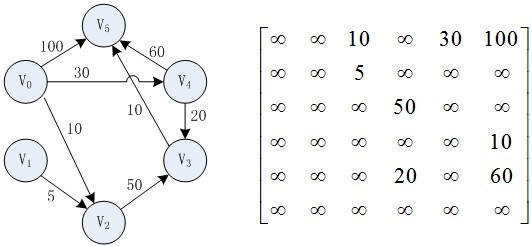
\includegraphics[width=240pt]{dijkstra.png}\\
\figcaption{有向图及其邻接矩阵}\label{fig:dijkstra}
\end{center}

运算过程中$v_0$到其余个顶点的最短路近,\fn{dist[]}向量的变化情况如表\ref{tab:dijkstra}所示(从一列到下一列只需要更新新加入点的邻接点)。

\begin{center}
\tabcaption{Dijkstra算法过程中dist[]向量的变化情况}
\label{tab:dijkstra}
\begin{tabular}{|c|ccccc|}
\hline
\textbf{\textbf{终点}} & \textbf{i=1} & \textbf{i=2} & \textbf{i=3} & \textbf{i=4} & \textbf{i=5}\\
\hline
$v_1$ & $\infty$ & $\infty$ & $\infty$ & $\infty$ & $\infty$\\
\hline
\multirow{2}{*}{$v_2$} & \textbf{10}          & & & & \\
                       & $\mathbf{(v_0,v_2)}$ & & & & \\
\hline
\multirow{2}{*}{$v_3$} & $\infty$ &          60     &     \textbf{50}          & & \\
                       &          & $(v_0,v_2,v_3)$ & $\mathbf{(v_0,v_4,v_5)}$ & & \\
\hline
\multirow{2}{*}{$v_4$} &     30      &      \textbf{30}     & & & \\
                       & $(v_0,v_4)$ & $\mathbf{(v_0,v_4)}$ & & & \\
\hline
\multirow{2}{*}{$v_5$} &     100     &     100     &       90        &         \textbf{60}          & \\
                       & $(v_0,v_5)$ & $(v_0,v_5)$ & $(v_0,v_4,v_5)$ & $\mathbf{(v_0,v_4,v_3,v_5)}$ & \\
\hline
$v_j$ & $v_2$ & $v_4$ & $v_3$ & $v_5$ & \\
\hline
$S$ & $(v_0,v_2)$ & $(v_0,v_2,v_4)$ & $(v_0,v_2,v_3,v_4)$ & $(v_0,v_2,v_3,v_4,v_5)$ & \\
\hline
\end{tabular}
\end{center}

Dijkstra算法的C++语言实现如下。

\subsubsection{代码}

\begin{Codex}[label=al_graph_dijkstra.cpp]
#include <iostream>
#include <queue>
#include <map>
#include <utility>
#include <climits>

using namespace std;

/** 边的权值类型,可以为int, float, double. */
typedef int graph_weight_t;

/** 顶点的编号,可以为char, int, string等. */
typedef char graph_vertex_id_t;

/**
 * @struct 图,用邻接表(Adjacency List).
 */
struct graph_t {
    int nv; // 顶点数
    int ne; // 边数
    // 邻接表,存放边的信息,如权重等
    map<graph_vertex_id_t, map<graph_vertex_id_t, graph_weight_t> > matrix;
};


/**
 * @brief Dijkstra算法求单源最短路径.
 * @param[in] g 图
 * @param[in] start 起点
 * @param[out] dist dist[v]存放的是起点到v的最短路径长度
 * @param[out] father father[v]存放的是最短路径上指向v的上一个顶点
 * @return 无
 */
void dijkstra(const graph_t &g, graph_vertex_id_t start,
        map<graph_vertex_id_t, graph_weight_t> &distance,
        map<graph_vertex_id_t, graph_vertex_id_t> &father) {
    /* 起点到顶点的最短距离. */
    typedef pair<graph_weight_t, graph_vertex_id_t> to_dist_t;

    // 小根堆
    priority_queue<to_dist_t, vector<to_dist_t>, greater<to_dist_t> > q;
    distance[start] = 0;  // 自己到自己,距离为0
    q.push(to_dist_t(0, start));
    while (!q.empty()) {
        const to_dist_t u = q.top(); q.pop();
        if (g.matrix.find(u.second) == g.matrix.end()) continue;

        for (map<graph_vertex_id_t, graph_weight_t>::const_iterator iter =
                g.matrix.at(u.second).begin();
                iter != g.matrix.at(u.second).end(); ++iter) {
            const graph_vertex_id_t v = iter->first;
            const graph_weight_t w = iter->second;

            if (!distance.count(v) || distance[u.second] + w < distance[v]) {
                distance[v] = distance[u.second] + w;
                father[v] = u.second;
                q.push(to_dist_t(distance[v], v));
            }
        }
    }
    return;
}

/**
 * @brief 打印从起点到终点的最短路径
 * @param[in] father Dijkstra计算好的father数组
 * @param[in] end 终点
 * @return 无
 */
void print_path(const map<graph_vertex_id_t, graph_vertex_id_t> &father,
        graph_vertex_id_t end) {
    if (!father.count(end)) {
        cout << end;
    } else {
        print_path(father, father.at(end));
        cout << "->" << end;
    }
}

/** 读取输入,构建图. */
void read_graph(graph_t &g) {
    cin >> g.ne;
    for (int i = 0; i < g.ne; ++i) {
        graph_vertex_id_t from, to;
        graph_weight_t weight;
        cin >> from >> to >> weight;
        g.matrix[from][to] = weight;
    }
}

/* test

输入数据:
8
A C 10
A E 30
A F 100
B C 5
C D 50
D F 10
E D 20
E F 60

输出:
A->C
A->E->D
A->E
A->E->D->F
*/
int main() {
    graph_t g;
    map<graph_vertex_id_t, graph_weight_t> distance;
    map<graph_vertex_id_t, graph_vertex_id_t> father;

    read_graph(g);

    dijkstra(g, 'A', distance, father);

    // 输出所有路径
    for(map<graph_vertex_id_t, graph_vertex_id_t>::const_iterator iter =
            father.begin(); iter != father.end();  ++iter) {
        if (iter->first != 'A') {
            print_path(father, iter->first);
            cout << endl;
        }
    }
    return 0;
}
\end{Codex}

\subsubsection{算法分析}
该算法包含了两个并列的for循环,第一个for循环做辅助数组的初始化工作,计算时间为$O(n)$,第二个for循环是二重嵌套循环,进行最短路径的求解工作,由于对图中几乎每个顶点都要做计算,每个顶点的又要对集合S内的顶点进行检测,对集合$V-S$内中的顶点进行修改,所以运算时间复杂度为$O(n^2)$。算法总的时间复杂度为$O(n^2)$。


\subsection{每点最短路径——Floyd算法}
Floyd算法的基本思想是:假设求从定点$v_i$到$v_j$的最短路径。初始时,若$v_i$与$v_j$之间存在边,则最短路径长度为此边的权值;若不存在边,则最短路径长度为无穷大。以后逐步在路径中加入顶点$k(k=0,1,...,n-1)$作为中间顶点,如果加入中间顶点后,得到的路径比原来的路径长度减少了,则以新路径代替原路径。

首先比较$(v_i,v_j)$和$(v_i,v_0,v_j)$的路径长度,取较短者为从$v_i$到$v_j$的中间顶点的序号不大于0的最短路径。如果$(v_i,v_0,v_j)$较短,则取$(v_i,v_0,v_j)$作为最短路径。假如在路径上再增加一个顶点$v_1$,也就是说,如果$(v_i,...,v_1)$和$(v_1,...,v_j)$分别是当前找到的中间定点的序号不大于0的最短路径,那么$(vi,...,v1,...,vj)$就有可能是从$v_i$到$v_j$的中间顶点的序号不大于1的最短路径,将它和已经得到的从$v_i$到$v_j$的中间顶点的序号不大于0的最短路径相比较,选出较短者作为从$v_i$到$v_j$的中间顶点的序号不大于1的最短路径。再增加一个顶点$v_2$,继续进行试探,依此类推。一般的,若$(v_i,...,v_k)$和$(v_k,...,v_j)$分别是从$v_i$到$v_k$和从$v_k$到$v_j$的中间定点的序号不大于$k-1$的最短路径,则将$(v_i,...,v_k,...,v_j)$和已经得到的从$v_i$到$v_j$的中间顶点的序号不大于$k-1$的最短路径相比,较短者便是从$v_i$到$v_j$的中间顶点的序号不大于$k$的最短路径。这样,在经过$n$次比较后,最后求得的必是从$v_i$到$v_j$的最短路径。

现定义一个$n$阶方阵序列,
$$
D^{(-1)}, D^{(0)} , D^{(1)},..., , D^{(k)},..., , D^{(n-1)}
$$
其中,
\begin{eqnarray}
D^{(-1)}[i][j] &=& \text{g->matrix}[i][j],  \nonumber \\
D^{(k)}[i][j] &=& \min\left\{D^{(k-1)}[i][j], D^{(k-1)}[i][k] + D^{(k-1)}[k][j]\right\},0 \leq k \leq n-1 \nonumber
\end{eqnarray}

上述公式中,$D^{(k)}[i][j]$是从$v_i$到$v_j$的中间顶点的序号不大于$k$的最短路径的长度;$D^{(n-1)}[i][j]$是从$v_i$到$v_j$的最短路径的长度。

例如,对图\ref{fig:floyd}所示的有向图及其邻接矩阵运行Floyd算法,

\begin{center}
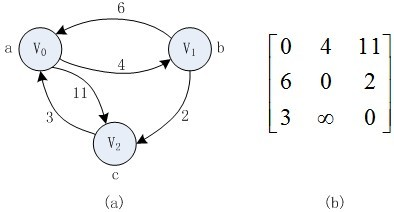
\includegraphics[width=180pt]{floyd.png}\\
\figcaption{有向图及其邻接矩阵}\label{fig:floyd}
\end{center}

运算过程中矩阵D的变化如表\ref{tab:floyd}所示。

\begin{center}
\tabcaption{Floyd算法过程中方阵和最短路径的变化}
\label{tab:floyd}
\begin{tabular}{|c|ccc|ccc|ccc|ccc|}
\hline
\multirow{2}{*}{$\mathbf{D}$} & \multicolumn{3}{|c|}{$\mathbf{D^{(0)}}$} & \multicolumn{3}{|c|}{$\mathbf{D^{(1)}}$} & \multicolumn{3}{|c|}{$\mathbf{D^{(2)}}$} & \multicolumn{3}{|c|}{$\mathbf{D^{(3)}}$} \\
 & 0 & 1 & 2 & 0 & 1 & 2 & 0 & 1 & 2 & 0 & 1 & 2 \\
\hline
0 & 0 & 4 & 11 & 0 & 4 & 11 & 0 & 4 & 6 & 0 & 4 & 6 \\
1 & 6 & 0 & 2 & 6 & 0 & 2 & 6 & 0 & 2 & 5 & 0 & 2 \\
2 & 3 & $\infty$ & 0 & 3 & 7 & 0 & 3 & 7 & 0 & 3 & 7 & 0 \\
\hline
\multirow{2}{*}{$\mathbf{P}$} & \multicolumn{3}{|c|}{$\mathbf{P^{(0)}}$} & \multicolumn{3}{|c|}{$\mathbf{P^{(1)}}$} & \multicolumn{3}{|c|}{$\mathbf{P^{(2)}}$} & \multicolumn{3}{|c|}{$\mathbf{P^{(3)}}$} \\
 & 0 & 1 & 2 & 0 & 1 & 2 & 0 & 1 & 2 & 0 & 1 & 2 \\
\hline
\multirow{2}{*}{0} & & A & A & & AB & A & & AB & AB & & AB & AB \\
                   & & B & C & & & C & & & C & & & C \\
\hline
\multirow{2}{*}{1} & B & & B & B & & B & B & & BC & BC & & BC \\
                   & A & & C & A & & C & A & & & A & & \\
\hline
\multirow{2}{*}{2} & C & & & C & CA & & C & CA & & CA & CA & \\
                   & A & & & A & B & & A & B & & & B & \\
\hline
\end{tabular}
\end{center}

Floyd算法的C语言实现如下。


\subsubsection{代码}

\begin{Codex}[label=am_graph_floyd.cpp]
#include <iostream>
#include <climits>  /* for INT_MAX */

using namespace std;

const int MAX_NV = 100; // 顶点数的最大值
/** 边的权值. */
typedef int graph_weight_t;
const int GRAPH_INF = INT_MAX / 2;   // 确保加法不溢出

/**
 *@struct 图,用邻接矩阵.
 */
struct graph_t {
    int nv; // 顶点数
    int ne; // 边数
    // 邻接矩阵,存放边的权重
    graph_weight_t matrix[MAX_NV][MAX_NV];
};


graph_t g;
/** dist[i][j]是顶点i和j之间最短路径长度 */
graph_weight_t dist[MAX_NV][MAX_NV];
/** path[i][j]是最短路径上i和j之间的顶点 */
int path[MAX_NV][MAX_NV];


/*
  * @brief Floyd算法求每点之间最短路径.
  * @param[in] g 图对象的指针
  * @param[out] dist dist[i][j]是顶点i和j之间最短路径长度
  * @param[out] path path[i][j]是最短路径上i和j之间的顶点
  * @return 无
  */
void floyd(const graph_t &g,
       graph_weight_t dist[][MAX_NV],
       int path[][MAX_NV]) {
    int i, j, k;
    const int n = g.nv;

    for(i = 0; i < n; i++) {
        for(j = 0; j < n; j++) {
            if(i != j) {
                dist[i][j] = g.matrix[i][j];
                path[i][j] = i;
            } else {
                dist[i][j] = 0;
                path[i][j] = -1;
            }
        }
    }
    for(k = 0; k < n; k++) {
        for(i = 0; i < n; i++) {
            for(j = 0; j < n; j++) {
                // i到j的路径上加入顶点k可以缩短路径长度
                if(dist[i][k] + dist[k][j] < dist[i][j]) {
                    dist[i][j] = dist[i][k] + dist[k][j];
                    path[i][j] = k;
                }
            }
        }
    }
}

/*
 * @brief 打印从u到v的最短路径
 * @param[in] u 起点
 * @param[in] v 终点
 * @param[in] path Floyd 计算好的path
 * @return 无
 */
static void print_path_r(int u, int v, const int path[][MAX_NV]) {
    if (path[u][v] == -1) {
        cout << (char)('A' + u);
    } else {
        print_path_r(u, path[u][v], path);
        cout << "->" << (char)('A' + v);
    }
}

/**
 * @brief 打印 u到其他所有点的最短路径
 * @param[in] path Dijkstra计算好的path
 * @param[in] n path的长度
 * @return 无
 */
void print_path(const graph_t &g, const int path[][MAX_NV]) {
    for (int i = 0; i < g.nv; i++) {
        for (int j = 0; j < g.nv; j++) {
            if (i != j) {
                print_path_r(i, j, path);
                cout << endl;
            }
        }
        cout << endl;
    }
}

/**
 * @brief 读取输入,构建图.
 */
void read_graph(graph_t &g) {
    cin >> g.nv >> g.ne;

    // 初始化图,所有节点间距离为无穷大
    for (int i = 0; i < g.nv; i++) {
        for (int j = 0; j < g.nv; j++) {
            g.matrix[i][j] = GRAPH_INF;
        }
    }

    for (int k = 0; k < g.ne; k++) { // 读取边信息
        char chx, chy;
        graph_weight_t w;

        cin >> chx >> chy >> w;
        g.matrix[chx - 'A'][chy - 'A'] = w;
    }
}

/* test

输入数据:
3 5
A B 4
A C 11
B A 6
B C 2
C A 3

输出:
A->B
A->B->C

B->C->A
B->C

C->A
C->A->B
*/
int main() {
    read_graph(g);
    /* 求两两之间的最短路径 */
    floyd(g, dist, path);
    print_path(g, path);
    return 0;
}
\end{Codex}

\subsubsection{算法分析}
该算法中有两个并列的for循环,第一个循环是个二重循环,用于初始化方阵$D$;第二个循环是个三重循环,逐步生成$D^{(0)}, D^{(1)} ,...,D^{(n-1)}$。所以算法总的时间复杂度为$O(n^3)$。

Dijkstra算法权值不能为负,Floyd权值可以为负,但环路之和不能为负。


\subsection{HDU 2544 最短路}
\subsubsection{描述}
在每年的校赛里,所有进入决赛的同学都会获得一件很漂亮的t-shirt。但是每当我们的工作人员把上百件的衣服从商店运回到赛场的时候,却是非常累的!所以现在他们想要寻找最短的从商店到赛场的路线,你可以帮助他们吗?

\subsubsection{输入}
输入包括多组数据。每组数据第一行是两个整数$N,M(N \leq 100,M \leq 10000)$,$N$表示成都的大街上有几个路口,标号为1的路口是商店所在地,标号为$N$的路口是赛场所在地,$M$则表示在成都有几条路。$N=M=0$表示输入结束。接下来$M$行,每行包括3个整数$A,B,C(1 \leq A,B \leq N,1 \leq C \leq 1000)$,表示在路口$A$与路口$B$之间有一条路,我们的工作人员需要$C$分钟的时间走过这条路。
输入保证至少存在1条商店到赛场的路线。

\subsubsection{输出}
对于每组输入,输出一行,表示工作人员从商店走到赛场的最短时间

\subsubsection{样例输入}
\begin{Code}
2 1
1 2 3
3 3
1 2 5
2 3 5
3 1 2
0 0
\end{Code}

\subsubsection{样例输出}
\begin{Code}
3
2
\end{Code}

\subsubsection{分析}
单源最短路径,用Dijkstra算法,将第\S\ref{sec:dijkstra}节中的代码稍加修改即可。

注意,街道是双向的,所以给边赋值时要对称赋值。

\subsubsection{代码}
\begin{Codex}[label=hdu_2544.cpp]
// HDU 2544 最短路, http://acm.hdu.edu.cn/showproblem.php?pid=2544
/** 边的权值类型. */
typedef int graph_weight_t;

/** 顶点的编号,可以为char, int, string等. */
typedef int graph_vertex_id_t;

// 等价于复制粘贴,这里为了节约篇幅,使用include,在OJ上提交时请用复制粘贴
#include "al_graph_dijkstra.cpp"  // 见“图->最短路径” 这节

/** 读取输入,构建图. */
void read_graph(graph_t &g) {
    cin >> g.nv >> g.ne;
    for (int i = 0; i < g.ne; ++i) {
        graph_vertex_id_t from, to;
        graph_weight_t weight;
        cin >> from >> to >> weight;
        g.matrix[from][to] = weight;
        g.matrix[to][from] = weight;  // 街道是双向的
    }
}


int main() {
    while(true) {
        graph_t g;
        map<graph_vertex_id_t, graph_weight_t> distance;
        map<graph_vertex_id_t, graph_vertex_id_t> father;

        read_graph(g);
        if (g.nv == 0 && g.ne == 0) break;

        dijkstra(g, 1, distance, father);
        cout << distance[g.nv] << endl;
    }

    return 0;
}
\end{Codex}

\subsubsection{相关的题目}
与本题相同的题目:
\begindot
\item HDU 2544 最短路, \myurl{http://acm.hdu.edu.cn/showproblem.php?pid=2544}
\myenddot

与本题相似的题目:
\begindot
\item POJ 2253 Frogger, \myurl{http://poj.org/problem?id=2253}
\item POJ 3268 Silver Cow Party, \myurl{http://poj.org/problem?id=3268}
\item POJ 1797 Heavy Transportation, \myurl{http://poj.org/problem?id=1797}
\item POJ 1847 Tram, \myurl{http://poj.org/problem?id=1847}
\myenddot


\subsection{POJ 1125 Stockbroker Grapevine}
\subsubsection{描述}
Stockbrokers are known to overreact to rumours. You have been contracted to develop a method of spreading disinformation amongst the stockbrokers to give your employer the tactical edge in the stock market. For maximum effect, you have to spread the rumours in the fastest possible way. 

Unfortunately for you, stockbrokers only trust information coming from their "Trusted sources" This means you have to take into account the structure of their contacts when starting a rumour. It takes a certain amount of time for a specific stockbroker to pass the rumour on to each of his colleagues. Your task will be to write a program that tells you which stockbroker to choose as your starting point for the rumour, as well as the time it will take for the rumour to spread throughout the stockbroker community. This duration is measured as the time needed for the last person to receive the information.

\subsubsection{输入}
Your program will input data for different sets of stockbrokers. Each set starts with a line with the number of stockbrokers. Following this is a line for each stockbroker which contains the number of people who they have contact with, who these people are, and the time taken for them to pass the message to each person. The format of each stockbroker line is as follows: The line starts with the number of contacts ($n$), followed by n pairs of integers, one pair for each contact. Each pair lists first a number referring to the contact (e.g. a '1' means person number one in the set), followed by the time in minutes taken to pass a message to that person. There are no special punctuation symbols or spacing rules. 

Each person is numbered 1 through to the number of stockbrokers. The time taken to pass the message on will be between 1 and 10 minutes (inclusive), and the number of contacts will range between 0 and one less than the number of stockbrokers. The number of stockbrokers will range from 1 to 100. The input is terminated by a set of stockbrokers containing 0 (zero) people. 

\subsubsection{输出}
For each set of data, your program must output a single line containing the person who results in the fastest message transmission, and how long before the last person will receive any given message after you give it to this person, measured in integer minutes. 

It is possible that your program will receive a network of connections that excludes some persons, i.e. some people may be unreachable. If your program detects such a broken network, simply output the message "disjoint". Note that the time taken to pass the message from person A to person B is not necessarily the same as the time taken to pass it from B to A, if such transmission is possible at all.

\subsubsection{样例输入}
\begin{Code}
3
2 2 4 3 5
2 1 2 3 6
2 1 2 2 2
5
3 4 4 2 8 5 3
1 5 8
4 1 6 4 10 2 7 5 2
0
2 2 5 1 5
7        
2 2 6 7 1
0  
3 1 5 2 8 4 7
0
2 2 9 4 10
2 3 8 4 7
2 5 8 6 3
7        
2 2 6 7 8
0  
3 1 5 2 8 4 7
0
2 2 9 4 10
2 3 8 4 7
2 5 8 6 3
0
\end{Code}

\subsubsection{样例输出}
\begin{Code}
3 2  
3 10
1 12
7 17
\end{Code}

\subsubsection{分析}
用Floyd算法求出每点之间的最短路径,输出距离最大的。

\subsubsection{代码}
\begin{Codex}[label=poj_1125.cpp]
// poj 1125 Stockbroker Grapevine, http://poj.org/problem?id=1125

// 等价于复制粘贴,这里为了节约篇幅,使用include,在OJ上提交时请用复制粘贴
#include "am_graph_floyd.cpp"  // 见“图->最短路径”这节

// 1. 修改范围
const int MAX_NV = 100; // 顶点数的最大值
// 2. 添加 max_len 数组
/** 存放每个点的最短路径的最长者 */
graph_weight_t max_len[MAX_NV];
// 3. 重写 read_graph()
// 4. 重写 main()

/** 读取输入,构建图. */
void read_graph(graph_t &g) {
    cin >> g.nv;
    g.ne = 0;

    /* 初始化图,所有节点间距离为无穷大 */
    for (int i = 0; i < g.nv; i++) {
        for (int j = 0; j < g.nv; j++) {
            g.matrix[i][j] = GRAPH_INF;
        }
    }

    /* 读取边信息 */
    for (int i = 0; i < g.nv; i++) {
        int m;
        cin >> m;
        g.ne += m;
        while (m--) {
            int j;
            graph_weight_t w;
            cin >> j >> w;
            --j;
            g.matrix[i][j] = w;
        }
    }
}

int main() {
    while (true) {
        read_graph(g);
        if (g.nv == 0) break;

        /* 求两两之间的最短路径 */
        floyd(g, dist, path);

        /* 找最短路径的最长着 */
        for (int i = 0; i < g.nv; i++) {
            max_len[i] = dist[i][distance(&dist[i][0],
                    max_element(&dist[i][0], &dist[i][0] + g.nv))];
        }
        /* 找 max_len 的最小者 */
        const int min_pos = distance(&max_len[0],
                min_element(&max_len[0], &max_len[0] + g.nv));

        if (max_len[min_pos] == GRAPH_INF) {
            cout << "disjoint" << endl;
        } else {
            cout << min_pos + 1 << " " << max_len[min_pos] << endl;
        }
    }
    return 0;
}
\end{Codex}

\subsubsection{相关的题目}
与本题相同的题目:
\begindot
\item POJ 1125 Stockbroker Grapevine, \myurl{http://poj.org/problem?id=1125}
\myenddot

与本题相似的题目:
\begindot
\item POJ 3615 Cow Hurdles, \myurl{http://poj.org/problem?id=3615}
\item POJ 3660 Cow Contest, \myurl{http://poj.org/problem?id=3660}
\item POJ 2502 Subway, \myurl{http://poj.org/problem?id=2502}
\item HDU 3631 Shortest Path, \myurl{http://acm.hdu.edu.cn/showproblem.php?pid=3631}
\myenddot


\section{拓扑排序} %%%%%%%%%%%%%%%%%%%%%%%%%%%%%%
由某个集合上的一个偏序得到该集合上的一个全序,这个操作称为\textbf{拓扑排序}。

拓扑序列的特点是:若有向边$<V_i, V_j>$是途中的弧,则在序列中顶点$V_i$必须排在顶点$V_j$之前。

如果用有向图表示一个工程,顶点表示活动,用有向边$<v_i,v_j>$表示活动必须先于活动进行。这种有向图叫做顶点表示活动的网络(Activity On Vertext Network),简称\textbf{AOV网络}。

检测AOV网络是否存在环的方法是对AOV网络构造其顶点的拓扑有序序列。拓扑排序的基本步骤是:
\begin{enumerate}
\item 在有向图中选一个没有前驱的顶点且输出之;
\item 从图中删除该顶点和所有以它为尾的弧线。
\end{enumerate}
重复以上两步,直至全部顶点输出,或当前图中不存在无前驱的顶点为止(这种情况说明图中存在环)。

拓扑排序的C语言实现如下。

\subsubsection{代码}

\begin{Codex}[label=am_graph_topo_sort.cpp]
#include <iostream>
#include <climits>  // for INT_MAX
#include <stack>

using namespace std;

/** 顶点数的最大值*/
const int MAX_NV = 100;
/** 边的权值,对无权图,用0或1表示是否相邻;对有权图,则为权值. */
typedef int graph_weight_t;
const graph_weight_t GRAPH_INF = INT_MAX;

/**
 *@struct
 *@brief 邻接矩阵.
 */
struct graph_t {
    int nv; // 顶点数
    int ne; // 边数
    // 邻接矩阵,存放边的信息,如权重等
    graph_weight_t matrix[MAX_NV][MAX_NV];
};

graph_t g;
/** 拓扑排序的结果. */
int topological[MAX_NV];

/*
  * @brief 拓扑排序.
  * @param[in] g 图对象的指针
  * @param[out] topological 保存拓扑排序的结果
  * @return 无环返回 true,有环返回 false
  */
bool topo_sort(const graph_t &g, int topological[]) {
    const int n = g.nv;
    int *in_degree = new int[n](); // in_degree[i]是顶点i的入度

    for (int i = 0; i < n; i++) {
        for (int j = 0; j < n; j++) {
            if (g.matrix[i][j] < GRAPH_INF)
                in_degree[j]++;
        }
    }

    stack<int> s;
    for(int i = 0; i < n; i ++) {
        if(in_degree[i] == 0)
            s.push(i);
    }

    int count = 0; /* 拓扑序列的元素个数*/
    while(!s.empty()) {
        const int u = s.top(); s.pop();
        topological[count++] = u;
        for (int i = 0; i < n; i++) if (g.matrix[u][i] < GRAPH_INF) {
            if(--in_degree[i] == 0) s.push(i);
        }
    }

    delete[] in_degree;
    if(count != n) { /* 有环*/
        return false;
    } else { /* 无环*/
        return true;
    }
}

/** 读取输入,构建图. */
void read_graph() {
    /* 读取节点和边的数目 */
    cin >> g.nv >> g.ne;

    /* 初始化图,所有节点间距离为无穷大 */
    for (int i = 0; i < g.nv; i++) {
        for (int j = 0; j < g.nv; j++) {
            g.matrix[i][j] = GRAPH_INF;
        }
    }

    /* 读取边信息 */
    for (int k = 0; k < g.ne; k++) {
        char chx, chy;
        graph_weight_t w;
        cin >> chx >> chy >> w;
        g.matrix[chx - 'A'][chy - 'A'] = w;
    }
}

/* test

输入数据:
6 8
A C 10
A E 30
A F 100
B C 5
C D 50
D 5 10
E D 20
E F 60

输出:
B A E F C D
*/
int main() {
    read_graph();
    /* 拓扑排序 */
    topo_sort(g, topological);
    for (int i = 0; i < g.nv; i++) {
        cout << (char)('A' + topological[i]) << " ";
    }
    return 0;
}
\end{Codex}

\subsubsection{算法分析}
对有$n$个顶点和$e$条边的AOV网络而言,求各顶点的入度所需时间为$O(e)$,建立零入度顶点栈所需时间为$O(n)$;在拓扑排序过程中,若有向图无环,每个顶进一次栈出一次栈,顶点入度减1的操作共执行了$e$次。所以总的时间复杂度为$O(n+e)$。

当有向图中无环时,也可以利用深度优先搜索进行拓扑排序。因为图中无环,深度优先遍历不会死循环。进行深度优先遍历时,最先退出DFS函数的顶点即为出度为零的顶点,是拓扑有序序列的最后一个顶点。由此,按退出DFS函数的先后次序记录下来的顶点序列即为逆向的拓扑有序序列。


\subsection{POJ 1094 Sorting It All Out}
\subsubsection{描述}
An ascending sorted sequence of distinct values is one in which some form of a less-than operator is used to order the elements from smallest to largest. For example, the sorted sequence $A, B, C, D$ implies that $A < B, B < C$ and $C < D$. in this problem, we will give you a set of relations of the form $A < B$ and ask you to determine whether a sorted order has been specified or not.

\subsubsection{输入}
Input consists of multiple problem instances. Each instance starts with a line containing two positive integers $n$ and $m$. the first value indicated the number of objects to sort, where $2 \leq n \leq 26$. The objects to be sorted will be the first $n$ characters of the uppercase alphabet. The second value $m$ indicates the number of relations of the form $A < B$ which will be given in this problem instance. Next will be $m$ lines, each containing one such relation consisting of three characters: an uppercase letter, the character "<" and a second uppercase letter. No letter will be outside the range of the first $n$ letters of the alphabet. Values of $n = m = 0$ indicate end of input.

\subsubsection{输出}
For each problem instance, output consists of one line. This line should be one of the following three: 

Sorted sequence determined after $xxx$ relations: $yyy...y$.

Sorted sequence cannot be determined. 

Inconsistency found after $xxx$ relations.

where $xxx$ is the number of relations processed at the time either a sorted sequence is determined or an inconsistency is found, whichever comes first, and $yyy...y$ is the sorted, ascending sequence.

\subsubsection{样例输入}
\begin{Code}
4 6
A<B
A<C
B<C
C<D
B<D
A<B
3 2
A<B
B<A
26 1
A<Z
6 6
A<F
B<D
C<E
F<D
D<E
E<F
0 0
\end{Code}

\subsubsection{样例输出}
\begin{Code}
Sorted sequence determined after 4 relations: ABCD.
Inconsistency found after 2 relations.
Sorted sequence cannot be determined.
Inconsistency found after 6 relations.
\end{Code}

\subsubsection{分析}
根据题目的要求,我们要每输入一次就要进行一次拓扑排序\fn{topological_sort()},这样才能做到不成功(即发现有环)时,能知道是哪步不成功,并且给出输出。

还有要注意的就是如果我们可以提前判断结果了,但后面还有输入没完成,那么我们必须继续完成输入,不然剩下的输入会影响下一次case的输入。

\subsubsection{代码}
\begin{Codex}[label=poj_1094.cpp]
// POJ 1094 Sorting It All Out, http://poj.org/problem?id=1094
#include <iostream>
#include <climits>  // for INT_MAX
#include <stack>

using namespace std;

/** 顶点数的最大值*/
const int MAX_NV  = 26;
/** 边的权值. */
typedef int graph_weight_t;
const int GRAPH_INF = INT_MAX;

/**
 *@struct 邻接矩阵.
 */
struct graph_t {
    int nv; // 顶点数
    int ne; // 边数
    // 邻接矩阵,存放边的信息,如权重等
    graph_weight_t matrix[MAX_NV][MAX_NV];
};

graph_t g;
/** 拓扑排序的结果. */
int topological[MAX_NV];

/**
  * @brief 拓扑排序.
  * @param[in] g 图对象的指针
  * @param[out] topological 保存拓扑排序的结果
  * @return 无环返回 1,有环返回 0,条件不足返回 -1
  */
int topo_sort(const graph_t *g, int topological[]) {
    const int n = g->nv;

    /* in_degree[i]是顶点i的入度 */
    int *in_degree = new int[n]();
    for (int i = 0; i < n; i++) {
        for (int j = 0; j < n; j++) {
            if (g->matrix[i][j] < GRAPH_INF)
                in_degree[j]++;
        }
    }

    stack<int> s;
    for(int i = 0; i < n; i ++) {
        if(in_degree[i] == 0) {
            s.push(i);
        }
    }

    int count = 0; // 拓扑序列的元素个数
    bool insufficient = false;  // 条件不足
    while(!s.empty()) {
        // 栈内应该始终只有一个元素
        if (s.size() > 1) insufficient = true;
        // 删除顶点u
        const int u = s.top(); s.pop();
        topological[count++] = u;
        --in_degree[u];  // 变成 -1,表示已经输出
        // 更新入度
        for (int i = 0; i < n; i++) if (g->matrix[u][i] < GRAPH_INF) {
            --in_degree[i];
        }
        // 选择入度为0的顶点
        for (int i = 0; i < n; i++) if (g->matrix[u][i] < GRAPH_INF) {
            if (in_degree[i] == 0) s.push(i);
        }
    }

    delete[] in_degree;
    if(count < n) { // 有环
        return 0;
    } else { // 无环
        if (insufficient) {  // 有孤立点,说明条件不足
            return -1;
        } else {
            return 1;
        }
    }
}

int main() {
    int m;  // m不一定是边的数目,因为输入边可能有重复

    /* 读取节点和边的数目 */
    while ((cin >> g.nv >> m) && g.nv > 0 && m > 0) {
        bool finished = false;  // 排序完成,结束,发现有环,可以提前结束

        // 初始化图,所有节点间距离为无穷大
        for (int i = 0; i < g.nv; i++)
            for (int j = 0; j < g.nv; j++)
                g.matrix[i][j] = GRAPH_INF;

        // 读取边信息
        for (int k = 0; k < m; k++) {
            string s;
            cin >> s;
            g.matrix[s[0] - 'A'][s[2] - 'A'] = 1;

            if (finished) continue;    // 完成,则 continue,消耗输入

            // 是否有环,0 表示有环
            const int ok = topo_sort(&g, topological);

            if (ok == 0) {  // 有环存在
                cout << "Inconsistency found after " << k+1 <<
                        " relations." << endl;
                finished = true;  // 提前结束,记住要继续消耗输入
            }
            if (ok == 1 && k) {
                cout << "Sorted sequence determined after " << k+1
                        << " relations: ";
                for (int i = 0; i < g.nv; i++) {
                    cout << (char)('A' + topological[i]);
                }
                cout << "." << endl;
                finished = true;
            }
            // ok==-1, continue
        }
        if (!finished) {
            cout << "Sorted sequence cannot be determined." << endl;
        }
    }
    return 0;
}
\end{Codex}

\subsubsection{相关的题目}
与本题相同的题目:
\begindot
\item POJ 1094 Sorting It All Out, \myurl{http://poj.org/problem?id=1094}
\myenddot

与本题相似的题目:
\begindot
\item POJ 3267 The Cow Lexicon, \myurl{http://poj.org/problem?id=3267}
\item POJ 3687 Labeling Balls, \myurl{http://poj.org/problem?id=3687}
\myenddot


\section{关键路径} %%%%%%%%%%%%%%%%%%%%%%%%%%%%%%
用有向边上的权值表示活动的持续时间,用顶点表示时间,这样的有向图叫做边表示的活动网络(Activity On Edge Network),简称\textbf{AOE网络}。

路径最长的路径叫做\textbf{关键路径}(Critical Path)。假设开始点为$v_1$,从$v_1$到$v_i$的最长路径长度叫做事件$v_i$的最早发生时间。这个事件决定了所有以$v_i$为尾的弧所表示的活动的最早开始时间。我们用$e(i)$表示活动$a_i$的最早开始时间。还可以定义一个活动的最迟开始时间$l(i)$,这是在不推迟整个工程完成的前提下,活动$a_i$最迟必须开始进行的时间。两者之差$l(i)-e(i)$意味着完成活动$a_i$的时间余量。我们把$l(i)=e(i)$的活动叫做关键活动。

设活动$a_i$由弧$<j, k>$表示,为了求得活动的$e(i)$和$l(i)$,首先应求得事件的最早发生时间$ve(j)$和最迟发生时间$vl(j)$,其持续时间记为$dut(<j, k>)$,则有如下关系
\begin{eqnarray}
e(i) &=& ve(j) \nonumber \\
l(i) &=& vl(k)-dut(<j, k>) \nonumber
\end{eqnarray}

求$ve(j)$和$vl(k)$需分两步进行:
\begin{enumerate}
\item 从$ve(0)=0$开始向前递推
$$
ve(j)=\max\left\{ve(i)+dut(<i, j>)\right\}, <i, j> \in T
$$
其中$T$是所有以顶点$j$为弧头的边的集合。
\item 从$vl(n-1)=ve(n-1)$起向后递推
$$
vl(j)=\min\left\{vl(k)-dut(<j, k>)\right\}, <j, k> \in S
$$
其中$S$是所有以顶点$j$为弧尾的边的集合。
\end{enumerate}

例如,对图\ref{fig:criticalpath}(a)所示AOE网络的计算过程如表\ref{tab:criticalpath}所示,可见$a_2$、$a_5$和$a_7$为关键活动,组成一条从起点到终点的关键路径,如图\ref{fig:criticalpath}(b)所示。

\begin{center}
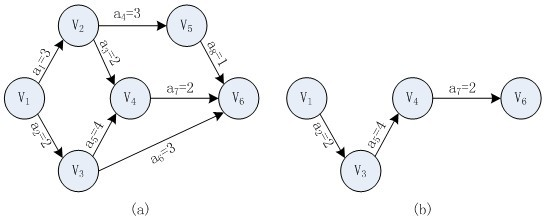
\includegraphics[width=240pt]{criticalpath.png}\\
\figcaption{有向图及其邻接矩阵}\label{fig:criticalpath}
\end{center}

\begin{center}
\tabcaption{图\ref{fig:criticalpath}(a)所示AOE网络的关键路径的计算过程}
\label{tab:criticalpath}
\begin{tabular}{|ccccc|cccc|}
\hline
\textbf{顶点} & \textbf{ve} & & \textbf{vl} & & \textbf{活动} & \textbf{e} & \textbf{l} & \textbf{l-e} \\
\hline
$v_1$ & 0 & \multirow{8}{*}{$\downarrow$} & 0 & \multirow{8}{*}{$\uparrow$} & $a_1$ & 0 & 1 & 1 \\
$v_2$ & 3 &                               & 4 &                             & $a_2$ & 0 & 0 & 0 \\
$v_3$ & 2 &                               & 2 &                             & $a_3$ & 3 & 4 & 1 \\
$v_4$ & 6 &                               & 6 &                             & $a_4$ & 3 & 4 & 1 \\
$v_5$ & 6 &                               & 7 &                             & $a_5$ & 2 & 2 & 0 \\
$v_6$ & 8 &                               & 8 &                             & $a_6$ & 2 & 5 & 3 \\
      &   &                               &   &                             & $a_7$ & 6 & 6 & 0 \\
      &   &                               &   &                             & $a_8$ & 6 & 7 & 1 \\
\hline
\end{tabular}
\end{center}


邻接矩阵上的关键路径的C语言实现如下。

\subsubsection{代码}

\begin{Codex}[label=am_graph_critical_path.cpp]
#include <iostream>
#include <climits>  /* for INT_MAX */
#include <stack>
#include <algorithm>

using namespace std;

/** 顶点数的最大值*/
const int MAX_NV = 100;
/** 边的权值,对无权图,用0或1表示是否相邻;对有权图,则为权值. */
typedef int graph_weight_t;
const graph_weight_t GRAPH_INF = INT_MAX;

/**
 *@struct 邻接矩阵.
 */
struct graph_t {
    int nv; /* 顶点数*/
    int ne; /* 边数*/
    /* 邻接矩阵,存放边的信息,如权重等*/
    graph_weight_t matrix[MAX_NV][MAX_NV];
};

graph_t g;
/** 拓扑排序的结果. */
int topological[MAX_NV];
/** 关键路径,其余顶点为-1. */
int path[MAX_NV];

/*
  * @brief 按照拓扑排序的顺序,计算所有顶点的最早发生时间 ve.
  * @param[in] g 图对象的指针
  * @param[out] topological 保存拓扑排序的结果
  * @param[out] ve 所有事件的最早发生时间
  * @return 无环返回 true,有环返回 false
  */
static bool toposort_ve(const graph_t &g, int topological[],
        graph_weight_t ve[]) {
    const int n = g.nv;

    /* in_degree[i]是顶点i的入度 */
    int *in_degree = new int[n]();
    for (int i = 0; i < n; i++) {
        for (int j = 0; j < n; j++) {
            if (g.matrix[i][j] < GRAPH_INF)
                in_degree[j]++;
        }
    }

    stack<int> s;
    for(int i = 0; i < n; i ++) {
        if(in_degree[i] == 0) {
            s.push(i);
        }
    }
    fill(ve, ve + n, 0);

    int count = 0; // 拓扑序列的元素个数
    while(!s.empty()) {
        // 删除顶点u
        const int u = s.top(); s.pop();
        topological[count++] = u;
        --in_degree[u];  // 变成 -1,表示已经输出
        // 更新入度
        for (int i = 0; i < n; i++) if (g.matrix[u][i] < GRAPH_INF) {
            --in_degree[i];
        }
        // 更新邻接点的 ve
        for (int i = 0; i < n; i++) if (g.matrix[u][i] < GRAPH_INF) {
            if (ve[i] < ve[u] + g.matrix[u][i])
                ve[i] = ve[u] + g.matrix[u][i];
        }
        // 选择入度为0的顶点
        for (int i = 0; i < n; i++) if (g.matrix[u][i] < GRAPH_INF) {
            if (in_degree[i] == 0) s.push(i);
        }
    }

    delete[] in_degree;

    if(count < n) return false; // 有环
    else          return true;  // 无环
}

/**
  * @brief 求关键路径,第一个顶点为起点,最后一个顶点为终点.
  * @param[in] g 图对象的指针
  * @param[out] ve 所有事件的最早发生时间
  * @param[inout] path 关键路径
  * @return 无环返回关键路径的顶点个数,有环返回 0
  */
int critical_path(const graph_t &g, int path[MAX_NV]) {
    int count = 0;    // 关键路径的顶点个数
    graph_weight_t *ve = new graph_weight_t[g.nv];
    graph_weight_t *vl = new graph_weight_t[g.nv];

    if (!toposort_ve(g, topological, ve)) return 0;  // 有环

    for (int i = 0; i < MAX_NV; i++) path[i] = -1;
    // 初始化 vl 为最大
    for (int i = 0; i < g.nv; i++) vl[i] = ve[g.nv-1];

    // 逆序计算vl
    for (int i = g.nv-1; i >=0; i--) {
        const int k = topological[i];
        for (int j = 0; j < g.nv; j++) {
            if (g.matrix[j][k] < GRAPH_INF) {
                if (vl[j] > vl[k] - g.matrix[j][k])
                    vl[j] = vl[k] - g.matrix[j][k];
            }
        }
    }
    for (int i = 0; i < g.nv; i++) {
        for (int j = 0; j < g.nv; j++) {
            const int e = ve[i];
            const int l = vl[j] - g.matrix[i][j];
            if (e == l) {
                if (i == 0) {
                    path[count++] = i;
                    path[count++] = j;
                } else {
                    path[count++] = j;
                }
            }
        }
    }

    delete[] ve;
    delete[] vl;
    return count;
}

/** 读取输入,构建图. */
void read_graph() {
    cin>> g.nv >> g.ne;

    // 初始化图,所有节点间距离为无穷大
    for (int i = 0; i < g.nv; i++)
        for (int j = 0; j < g.nv; j++)
            g.matrix[i][j] = GRAPH_INF;

    for (int k = 0; k < g.ne; k++) {  // 读取边信息
        char chx, chy;
        graph_weight_t w;
        cin >> chx >> chy >> w;
        g.matrix[chx - 'A'][chy - 'A'] = w;
    }
}

/* test

输入数据:
6 8
A B 3
A C 2
C D 4
B D 2
C F 3
B E 3
E F 1
D F 2

输出: A C D F

*/
int main() {
    read_graph();
    /* 拓扑排序 */
    const int count = critical_path(g, path);
    for (int i = 0; i < count; i++) {
        cout << (char)('A' + path[i]) << " ";
    }
    return 0;
}
\end{Codex}

\subsubsection{算法分析}
一次正向,复杂度为$O(n^2)$,一次逆向,复杂度为$O(n^2)$,因此,该算法的复杂度为$O(n^2)$。

\chapter{数学方法与常见模型}
数学对于算法很重要。没有好的数学基础,很难在算法上达到一定高度。本章介绍算法竞赛中常用的数学方法和模型。

\section{数论} %%%%%%%%%%%%%%%%%%%%%%%%%%%%%%

\subsection{欧几里德算法}

求最大公约数(greates common divisor)有很多方法,最经典的方法是欧几里德算法(Euclidean algorithm\footnote{\myurl{http://en.wikipedia.org/wiki/Euclid_algorithm}}),又称辗转相除法。

\begin{Codex}[label=gcd.c]
/**
 * @brief 求最大公约数,欧几里德算法,也即辗转相除法
 *
 * @param[in] a a
 * @param[in] b b
 * @return a和b的最大公约数
 */
unsigned int gcd(unsigned int a, unsigned int b) {
    if (b == 0) return a;
    return gcd(b, a % b);
}

/**
 * @brief 求最大公约数,欧几里德算法,迭代版本
 *
 * @param[in] a a
 * @param[in] b b
 * @return a和b的最大公约数
 */
unsigned int gcd1(unsigned int a, unsigned int b) {
    while (b != 0) {
        unsigned int tmp = b;
        b = a % b;
        a = tmp;
    }
    return a;
}

/**
 * @brief 求最大公约数,欧几里德算法,迭代版本,基于减法
 *
 * @param[in] a a
 * @param[in] b b
 * @return a和b的最大公约数
 */
unsigned int gcd2(unsigned int a, unsigned int b) {
    while (a != b) {
        if (a > b) {
            a -= b;
        } else {
            b -= a;
        }
    }
    return a;
}
\end{Codex}

求出了最大公约数,可以利用它来求最小公倍数(least common multiple), $\mathrm{lcm}(a,b)=a \times b / \gcd(a,b)$。

\subsubsection{例题}
\begindot
\item wikioi 1212 最大公约数 ,\myurl{http://www.wikioi.com/problem/1212/}
\myenddot


\subsection{扩展欧几里德算法}
定理:对于不完全为$0$的非负整数$a,b$,必然存在整数对 $x,y$ ,使得 $\gcd(a,b)=ax+by$。

这里$x$和$y$不一定是正数。扩展欧几里德算法(Extended Euclidean algorithm\footnote{\myurl{http://en.wikipedia.org/wiki/Extended_Euclidean_algorithm}})就是用来求$x$和$y$的。

\begin{Codex}[label=ex_gcd.c]
/**
 * @brief 扩展欧几里德算法
 * @param[in] a a
 * @param[in] b b
 * @param[out] x
 * @param[out] y
 * @return gcd(a,b)
 */
unsigned int ex_gcd(unsigned int a, unsigned int b, int *x, int *y) {
    if(b == 0) {
        *x = 1; *y = 0; return a;
    } else {
        const unsigned int tmp = ex_gcd(b, a % b, y, x);
        *y -= (*x)*(a/b);
        return tmp;
    }
}
\end{Codex}

扩展欧几里德算法的应用主要有以下三个:
\begindot
\item 求解不定方程;
\item 求解模线性方程(线性同余方程);
\item 求解模的逆元;
\myenddot


\subsubsection{求解不定方程}
求不定方程$ax+by=c$的整数解$x,y$,其中$a > b \geq c \geq 0$。

设$g=\gcd(a,b)$,方程$ax+by=g$的一组解是$(x_0,y_0)$,则当$c$是$g$的倍数时$ax+by=c$的一组解是$(x_0,y_0)$。证明略。

\begin{Code}
/**
 * @brief 求解不定方程ax+by=c
 * @param[in] a a
 * @param[in] b b
 * @param[in] c c
 * @param[out] x x
 * @param[out] y y
 * @return 是否有解,1表示有解,0表示无解
 */
int linear_equation(unsigned int a, unsigned int b, unsigned int c,
        int *x, int *y) {
    unsigned int k;
    const unsigned int g = ex_gcd(a, b, x, y);
    if (c % g) return 0;

    k = c / g;
    (*x) *= k; (*y) *= k;
    return 1;
}
\end{Code}


\subsubsection{求解模线性方程}
解方程$ax \equiv b\bmod n$,其中$a,b,n$是正整数。

$ax \equiv b\bmod n$的含义是“$ax$和$b$除以$n$的余数相同”,设这个倍数为$y$,则$ax-b=ny$,这恰好就是前面介绍过的不定方程。接下来的步骤就不用说了吧。

\begin{Code}
/**
 * @brief 求解模线性方程 ax = b mod n
 * @param[in] a
 * @param[in] b
 * @param[in] n n>0
 */
int modular_linear_equation(unsigned int a, unsigned int b, unsigned int n) {
    int x, y, x0, i;
    unsigned int k;
    unsigned int g = ex_gcd(a, n, &x, &y);
    if(b % g) return 0;

    k = b / g;
    x0 = (k * x) % n;   //特解
    for (i = 0; i < g; i++)
        printf("%d\n", (x0 + i * (n/g)) % n);
    return 1;
}
\end{Code}


\subsubsection{求解模的逆元}
有一个特殊情况要引起读者重视,当$b=1$时,$ax \equiv 1\bmod n$的解称为$a$关于模$n$的逆(inverse),它类似于“倒数”的概念。什么时候$a$的逆存在呢?根据上面的讨论,方程$ax-ny=1$要有解,这样,1必须是$\gcd(a,n)$的倍数,因此$a$和$n$必须互素。

\subsection{素数判定}
素数判定,又称素数测试(Primality test\footnote{\myurl{http://en.wikipedia.org/wiki/Primality_test}}),即给定一个正整数$n$,判断它是否是素数。

\subsubsection{暴力枚举法}
从2到$n$,依次作为除数,让$n$除以它们,只要有一个能整除$n$,则$n$不是素数。

\begin{Code}
/**
 * @brief 判断正整数n是否是素数
 * @param[in] n 正整数
 * @return 是,返回1,否,返回0
 */
int is_prime(unsigned int n) {
    int i;
    if (n < 2) return 0;
    for (i = 2; i < n; i++) {
        if (n % i == 0) return 0;
    }
    return 1;
}
\end{Code}

可以稍微做一点改进,从1到$\sqrt n$,依次作为除数。

\begin{Code}
/**
 * @brief 判断正整数n是否是素数,上界改为sqrt(n)
 * @param[in] n 正整数
 * @return 是,返回1,否,返回0
 */
int is_prime(unsigned int n) {
    int i;
    if (n < 2) return 0;
    const int upper = sqrt(n);

    for (i = 2; i <= upper; i++) {
        if (n % i == 0) return 0;
    }
    return 1;
}

/**
 * @brief 判断正整数n是否是素数,上界改为sqrt(n),但不使用sqrt()函数
 * @param[in] n 正整数
 * @return 是,返回1,否,返回0
 */
int is_prime1(unsigned int n) {
    int i;
    if (n < 2) return 0;
    for (i = 2; i*i <= n; i++) {
        if (n % i == 0) return 0;
    }
    return 1;
}
\end{Code}

\subsubsection{Eratosthenes筛法}
更高效的素数判定方法应该是预先计算出一张素数表,当判断一个数是否是素数时,直接查表即可。

怎样计算?用Eratosthenes筛法(Sieve of Eratosthenes\footnote{\myurl{http://en.wikipedia.org/wiki/Sieve_of_Eratosthenes}})

给出要筛数值的范围$n$,找出$\sqrt{n}$以内的素数$p_{1},p_{2},\dots,p_{k}$。先用2去筛,即把2留下,把2的倍数剔除掉;再用下一个质数,也就是3筛,把3留下,把3的倍数剔除掉;接下去用下一个质数5筛,把5留下,把5的倍数剔除掉;不断重复下去......。

\begin{Code}
#define MAXN 30000
/** prime_table[i]==1表示i是素数,等于0则不是素数 */
int prime_table[MAXN+1];

void compute_prime_table() {
    int i, j;
    const int upper = sqrt(MAXN);

    for (i = 2; i <= MAXN; i++) prime_table[i] = 1;
    prime_table[0] = 0;
    prime_table[1] = 0;

    for (i = 2; i < upper; i++) if(prime_table[i]) {
        for (j = 2; j * i <= MAXN; j++) prime_table[j*i] = 0;
    }
}

int is_prime(unsigned int n) {
    return prime_table[n];
}
\end{Code}

\subsubsection{暴力枚举法优化版}
下面这段代码是从 GNU GMP(\myurl{http://gmplib.org/})的源代码中抠出来的。

\begin{Code}
int is_prime(unsigned int n) {
    unsigned int q, r, d;    /* 商,余数,除数 */

    /* 把这个常数展开成二进制就容易理解了 */
    if (n < 32) return (0xa08a28acUL >> n) & 1;
    if ((n & 1) == 0) return 0;
    if (n % 3 == 0) return 0;
    if (n % 5 == 0) return 0;
    if (n % 7 == 0) return 0;

    for (d = 11;;) {
        q = n / d;
        r = n - q * d;
        if (q < d) return 1;    /* 保证 d 不超过 sqrt(n) */
        if (r == 0) break;

        d += 2;
        q = n / d;
        r = n - q * d;
        if (q < d) return 1;
        if (r == 0) break;

        d += 4;
    }
    return 0;
}
\end{Code}


\subsubsection{例题}
\begindot
\item wikioi 1430 素数判定,\myurl{http://www.wikioi.com/problem/1430/}
\myenddot


\subsection{大整数取模} %%%%%%%%%%%%%%%%%%%%%%%%%%%%%%
\subsubsection{描述}
求$a \bmod b, 1 \leq a \leq 10^{1000},1 \leq b \leq 100000$。

\subsubsection{输入}
每行2个整数$a$和$b$

\subsubsection{输出}
对每一行输出结果 $a \bmod b$

\subsubsection{样例输入}
\begin{Code}
2 3
12 7
152455856554521 3250
\end{Code}

\subsubsection{样例输出}
\begin{Code}
2
5
1521
\end{Code}

\subsubsection{代码}
\begin{Codex}[label=bigint_mod.c]
#include<stdio.h>
#include<string.h>

/* 一个数组元素表示4个十进制位,即数组是万进制的 */
#define BIGINT_MOD 10000
#define MOD_LEN 4
#define MAX_LEN (1000/MOD_LEN+1)  /* 整数的最大位数 */

char    a[MAX_LEN * MOD_LEN];
int     x[MAX_LEN], y;

/**
 * @brief 将输入的字符串转化为大整数,用数组表示,低位在低地址.
 * @param[in] s 输入的字符串
 * @param[out] x 大整数
 * @return 无
 */
void bigint_input(const char s[], int x[]) {
    int i, j = 0;
    const int len = strlen(s);
    for (i = 0; i < MAX_LEN; i++) x[i] = 0;

    /* for (i = len - 1; i >= 0; i--) a[j++] = s[i] - '0'; */
    for (i = len; i > 0; i -= MOD_LEN) {  /* [i-MOD_LEN, i) */
        int temp = 0;
        int k;
        const int low = i-MOD_LEN > 0 ? i-MOD_LEN : 0;
        for (k = low; k < i; k++) {
            temp = temp * 10 + s[k] - '0';
        }

        x[j++] = temp;
    }
}

/**
 * @brief 计算 x mod y
 * @param[in] x 大整数
 * @param[in] y 模
 * @return x mod y
 */
int bigint_mod(const int x[MAX_LEN], int y) {
    int ret = 0;
    int i;
    for (i = MAX_LEN-1; i >= 0; i--) {
        ret = (ret * BIGINT_MOD + x[i]) % y;
    }
    return ret;
}

int main() {
    while(scanf("%s%d", a, &y) > 1) {
        bigint_input(a, x);
        printf("%d\n", bigint_mod(x, y));
    }
    return 0;
}
\end{Codex}

\subsubsection{相关的题目}
与本题相同的题目:
\begindot
\item HDU 1212 Big Number, \myurl{http://acm.hdu.edu.cn/showproblem.php?pid=1212}
\myenddot

与本题相似的题目:
\begindot
\item  None
\myenddot


\section{组合数学} %%%%%%%%%%%%%%%%%%%%%%%%%%%%%%


\chapter{大整数运算}
在32位CPU下,C/C++中的int能表示的范围是$[-2^{32}, 2^{32}-1]$,unsigned int能表示的范围是$[0, 2^{32}]$。所以,int 和 unsigned int都不能保存超过 10位的整数(解方程$10^x \leq 2^{32}$,可得$x \leq 9.63$)。有时我们需要参与运算的整数,可能会远远不止10位,我们称这种基本数据类型无法表示的整数为大整数。如何表示和存放大整数呢?基本的思想是:用数组模拟大整数。一个数组元素,存放大整数中的一位。

例如,一个200位的十进制整数,可以用 \fn{int x[200]}来表示,一个数组元素对应一个位。这样做有点浪费空间,因为一个int可以表示的范围远远大于10。因此,我们可以用一个数组元素,表示4个数位(一个int可以表示的范围也远远大于10000,为什么一个数组元素只表示4个数位,可不可以表示9个数位?留给读者思考),这时,数组不再是10进制,而是10000进制。使用万进制,数组长度可以缩减到原来的1/4。

\section{大整数加法} %%%%%%%%%%%%%%%%%%%%%%%%%%%%%%
\subsubsection{描述}
求两个非负的大整数相加的和。

\subsubsection{输入}
有两行,每行是一个不超过200位的非负整数,可能有多余的前导0。

\subsubsection{输出}
一行,即相加后的结果。结果里不能有多余的前导0,即如果结果是342,那么就不能输出为0342。

\subsubsection{样例输入}
\begin{Code}
22222222222222222222 
33333333333333333333
\end{Code}

\subsubsection{样例输出}
\begin{Code}
55555555555555555555
\end{Code}

\subsubsection{代码}
\begin{Codex}[label=bigint_add.c]
#include<stdio.h>
#include<string.h>

/* 一个数组元素表示4个十进制位,即数组是万进制的 */
#define BIGINT_RADIX 10000
#define RADIX_LEN 4
#define MAX_LEN (200/RADIX_LEN+1)  /* 整数的最大位数 */

char    a[MAX_LEN * RADIX_LEN], b[MAX_LEN * RADIX_LEN];
int     x[MAX_LEN], y[MAX_LEN], z[MAX_LEN + 1];

/**
 * @brief 打印大整数.
 * @param[in] x 大整数,用数组表示,低位在低地址
 * @param[in] n 数组x的长度
 * @return 无
 */
void bigint_print(const int x[], const int n) {
    int i;
    int start_output = 0;  /* 用于跳过前导0 */
    for (i = n - 1; i >= 0; --i) {
        if (start_output) {  /* 如果多余的0已经都跳过,则输出 */
            printf("%04d", x[i]);
        } else if (x[i] > 0) {
            printf("%d", x[i]);
            start_output = 1; /* 碰到第一个非0的值,就说明多余的0已经都跳过 */
        }
    }

    if(!start_output) printf("0");  /* 当x全为0时 */
}

/**
 * @brief 将输入的字符串转化为大整数.
 * @param[in] s 输入的字符串
 * @param[out] x 大整数,用数组表示,低位在低地址
 * @return 无
 */
void bigint_input(const char s[], int x[]) {
    int i, j = 0;
    const int len = strlen(s);
    for (i = 0; i < MAX_LEN; i++) x[i] = 0;

    // for (i = len - 1; i >= 0; i--) a[j++] = s[i] - '0';
    for (i = len; i > 0; i -= RADIX_LEN) {  /* [i-RADIX_LEN, i) */
        int temp = 0;
        int k;
        const int low = i-RADIX_LEN > 0 ? i-RADIX_LEN : 0;
        for (k = low; k < i; k++) {
            temp = temp * 10 + s[k] - '0';
        }

        x[j++] = temp;
    }
}

/**
 * @brief 大整数加法
 * @param[in] x x
 * @param[in] y y
 * @param[out] z z=x+y
 * @return 无
 */
void bigint_add(const int x[], const int y[], int z[]) {
    int i;
    for (i = 0; i < MAX_LEN + 1; i++) z[i] = 0;

    for (i = 0; i < MAX_LEN; i++) {  /* 逐位相加 */
        z[i] += x[i] + y[i];
        if (z[i] >= BIGINT_RADIX) {  /* 看是否要进位 */
            z[i] -= BIGINT_RADIX;
            z[i+1] ++;  /* 进位 */
        }
    }
}


int main() {
    scanf("%s%s", a, b);

    bigint_input(a, x);
    bigint_input(b, y);

    bigint_add(x, y, z);
    bigint_print(z, MAX_LEN + 1);
    printf("\n"); 
    return 0;
}
\end{Codex}

\subsubsection{相关的题目}
与本题相同的题目:
\begindot
\item 《程序设计导引及在线实践》\footnote{李文新,程序设计导引及在线实践, 清华大学出版社, 2007}第144页7.1节
\item 百练 2981 大整数加法, \myurl{http://poj.grids.cn/practice/2981/}
\myenddot

与本题相似的题目:
\begindot
\item  None
\myenddot


\section{大整数减法} %%%%%%%%%%%%%%%%%%%%%%%%%%%%%%
\subsubsection{描述}
求两个非负的大整数相减的差。

\subsubsection{输入}
第1行是测试数据的组数T,每组测试数据占2行,第1行是被减数a,第2行是减数b(a > b),每行数据不超过100个字符,没有多余的前导0。每组测试数据之间有一个空行。

\subsubsection{输出}
每组测试数据输出一行,即相应的差

\subsubsection{样例输入}
\begin{Code}
2
9999999999999999999999999999999999999
9999999999999

5409656775097850895687056798068970934546546575676768678435435345
1
\end{Code}

\subsubsection{分析}
模拟小学生列竖式做加法,从个位开始逐位相加,超过或达到10(这里用万进制,则是10000)则进位。

两个200位的大整数相加,结果可能会有201位。

\subsubsection{样例输出}
\begin{Code}
9999999999999999999999990000000000000
5409656775097850895687056798068970934546546575676768678435435344
\end{Code}

\subsubsection{代码}
\begin{Codex}[label=bigint_sub.c]
#include<stdio.h>
#include<string.h>

/* 一个数组元素表示4个十进制位,即数组是万进制的 */
#define BIGINT_RADIX 10000
#define RADIX_LEN 4
#define MAX_LEN (100/RADIX_LEN+1)  /* 整数的最大位数 */

char    a[MAX_LEN * RADIX_LEN], b[MAX_LEN * RADIX_LEN];
int     x[MAX_LEN], y[MAX_LEN], z[MAX_LEN];

/**
 * @brief 打印大整数.
 * @param[in] x 大整数,用数组表示,低位在低地址
 * @param[in] n 数组x的长度
 * @return 无
 */
void bigint_print(const int x[], const int n) {
    int i;
    int start_output = 0;  /* 用于跳过前导0 */
    for (i = n - 1; i >= 0; --i) {
        if (start_output) {  /* 如果多余的0已经都跳过,则输出 */
            printf("%04d", x[i]);
        } else if (x[i] > 0) {
            printf("%d", x[i]);
            start_output = 1; /* 碰到第一个非0的值,就说明多余的0已经都跳过 */
        }
    }

    if(!start_output) printf("0");  /* 当x全为0时 */
}

/**
 * @brief 将输入的字符串转化为大整数.
 * @param[in] s 输入的字符串
 * @param[out] x 大整数,用数组表示,低位在低地址
 * @return 无
 */
void bigint_input(const char s[], int x[]) {
    int i, j = 0;
    const int len = strlen(s);
    for (i = 0; i < MAX_LEN; i++) x[i] = 0;

    // for (i = len - 1; i >= 0; i--) a[j++] = s[i] - '0';
    for (i = len; i > 0; i -= RADIX_LEN) {  /* [i-RADIX_LEN, i) */
        int temp = 0;
        int k;
        const int low = i-RADIX_LEN > 0 ? i-RADIX_LEN : 0;
        for (k = low; k < i; k++) {
            temp = temp * 10 + s[k] - '0';
        }

        x[j++] = temp;
    }
}

/**
 * @brief 大整数减法.
 *
 * @param[in] x x
 * @param[in] y y, x>y
 * @param[out] z z=x-y
 * @return 无
 */
void bigint_sub(const int x[], const int y[], int z[]) {
    int i;
    for (i = 0; i < MAX_LEN; i++) z[i] = 0;

    for (i = 0; i < MAX_LEN; i++) {  /* 逐位相减 */
        z[i] += x[i] - y[i];
        if (z[i] < 0) {  /* 看是否要借位 */
            z[i] += BIGINT_RADIX;
            z[i+1] --;  /* 借位 */
        }
    }
}

int main() {
    int T;    
    scanf("%d", &T);

    while (T-- > 0) {
        scanf("%s%s",a,b);

        bigint_input(a, x);
        bigint_input(b, y);

        bigint_sub(x, y, z);
        bigint_print(z, MAX_LEN);
        printf("\n"); 
    }
    return 0;
}
\end{Codex}

\subsubsection{相关的题目}
与本题相同的题目:
\begindot
\item 百练 2736 大整数减法, \myurl{http://poj.grids.cn/practice/2736/}
\myenddot

与本题相似的题目:
\begindot
\item  None
\myenddot


\section{大整数乘法} %%%%%%%%%%%%%%%%%%%%%%%%%%%%%%
\label{sec:bigintmul}
\subsubsection{描述}
求两个非负的大整数相乘的积。

\subsubsection{输入}
有两行,每行是一个不超过200位的非负整数,没有多余的前导0。 

\subsubsection{输出}
一行,即相乘后的结果。结果里不能有多余的前导0。 

\subsubsection{样例输入}
\begin{Code}
12345678900
98765432100
\end{Code}

\subsubsection{样例输出}
\begin{Code}
1219326311126352690000
\end{Code}

\subsubsection{分析}
两个200位的数相乘,积最多会有400位。

计算的过程基本上和小学生列竖式做乘法相同。为编程方便,并不急于处理进位,而将进位问题留待最后统一处理。 

现以$835 \times 49$为例来说明程序的计算过程。

先算$835 \times9$。$5 \times 9$得到45个1 ,$3 \times 9$ 得到27 个10,$8 \times 9$ 得到 72个100。由于不急于处理进位,所以$835 \times 9$ 算完后,aResult 如下:
\begin{center}
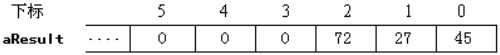
\includegraphics[width=260pt]{bigintmul1.png}\\
\end{center}

接下来算$4 \times 5$ 。此处$4 \times 5$的结果代表20个10 ,因此要 aResult[1]+=20,变为:
\begin{center}
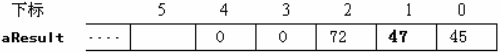
\includegraphics[width=260pt]{bigintmul2.png}\\
\end{center}

再下来算$4 \times 3$。此处$4 \times 3$的结果代表12个100,因此要 aResult[2]+= 12,变为:
\begin{center}
\includegraphics[width=260pt]{bigintmul3.png}\\
\end{center}

最后算$4 \times 8$。此处$4 \times 8$的结果代表32个1000 ,因此要 aResult[3]+= 32,变为:
\begin{center}
\includegraphics[width=260pt]{bigintmul4.png}\\
\end{center}

乘法过程完毕。接下来从 aResult[0] 开始向高位逐位处理进位问题。aResult[0]留下5,把4 加到aResult[1]上,aResult[1]变为 51 后,应留下 1 ,把5 加到aResult[2]上……最终使得aResult 里的每个元素都是 1 位数,结果就算出来了:
\begin{center}
\includegraphics[width=260pt]{bigintmul5.png}\\
\end{center}

总结一个规律,即一个数的第i位和另一个数的第j位相乘所得的数,一定是要累加到结果的第i+j位上。这里i, j都是从右往左,从0开始数。

\subsubsection{代码}
\begin{Codex}[label=bigint_mul.c]
#include<stdio.h>
#include<string.h>

/* 一个数组元素表示4个十进制位,即数组是万进制的 */
#define BIGINT_RADIX 10000
#define RADIX_LEN 4
#define MAX_LEN (200/RADIX_LEN+1)  /* 整数的最大位数 */

char    a[MAX_LEN * RADIX_LEN], b[MAX_LEN * RADIX_LEN];
int     x[MAX_LEN], y[MAX_LEN], z[MAX_LEN * 2];

/**
 * @brief 打印大整数.
 * @param[in] x 大整数,用数组表示,低位在低地址
 * @param[in] n 数组x的长度
 * @return 无
 */
void bigint_print(const int x[], const int n) {
    int i;
    int start_output = 0;  /* 用于跳过前导0 */
    for (i = n - 1; i >= 0; --i) {
        if (start_output) {  /* 如果多余的0已经都跳过,则输出 */
            printf("%04d", x[i]);
        } else if (x[i] > 0) {
            printf("%d", x[i]);
            start_output = 1; /* 碰到第一个非0的值,就说明多余的0已经都跳过 */
        }
    }

    if(!start_output) printf("0");  /* 当x全为0时 */
}

/**
 * @brief 将输入的字符串转化为大整数.
 * @param[in] s 输入的字符串
 * @param[out] x 大整数,用数组表示,低位在低地址
 * @return 无
 */
void bigint_input(const char s[], int x[]) {
    int i, j = 0;
    const int len = strlen(s);
    for (i = 0; i < MAX_LEN; i++) x[i] = 0;

    // for (i = len - 1; i >= 0; i--) a[j++] = s[i] - '0';
    for (i = len; i > 0; i -= RADIX_LEN) {  /* [i-RADIX_LEN, i) */
        int temp = 0;
        int k;
        const int low = i-RADIX_LEN > 0 ? i-RADIX_LEN : 0;
        for (k = low; k < i; k++) {
            temp = temp * 10 + s[k] - '0';
        }

        x[j++] = temp;
    }
}

/**
 * @brief 大整数乘法.
 * @param[in] x x
 * @param[in] y y
 * @param[out] z z=x*y
 * @return 无
 */
void bigint_mul(const int x[], const int y[], int z[]) {
    int i, j;
    for (i = 0; i < MAX_LEN * 2; i++) z[i] = 0;

    for (i = 0; i < MAX_LEN; i++) {
        for (j = 0; j < MAX_LEN; j++) { /*用y[i],去乘以x的各位*/
            z[i + j] += y[i] * x[j]; /* 两数第i, j位相乘,累加到结果的第i+j位 */

            if (z[i + j] >= BIGINT_RADIX) { /* 看是否要进位 */
                z[i + j + 1] += z[i + j] / BIGINT_RADIX; /* 进位 */
                z[i + j] %= BIGINT_RADIX;
            }
        }
    }
}


int main() {
    scanf("%s%s", a, b);

    bigint_input(a, x);
    bigint_input(b, y);

    bigint_mul(x, y, z);
    bigint_print(z, MAX_LEN * 2);
    printf("\n");
    return 0;
}
\end{Codex}

\subsubsection{相关的题目}
与本题相同的题目:
\begindot
\item 《程序设计导引及在线实践》\footnote{李文新,程序设计导引及在线实践, 清华大学出版社, 2007}第146页7.2节
\item 百练 2980 大整数乘法, \myurl{http://poj.grids.cn/practice/2980/}
\myenddot

与本题相似的题目:
\begindot
\item  None
\myenddot


\section{大整数除法} %%%%%%%%%%%%%%%%%%%%%%%%%%%%%%
\subsubsection{描述}
求两个非负的大整数相除的商。

\subsubsection{输入}
第1行是测试数据的组数T,每组测试数据占2行,第1行是被除数,第2行是除数,每行数据不超过100 个字符。每组测试数据之间有一个空行。

\subsubsection{输出}
每组测试数据输出一行,即相应的整数商

\subsubsection{样例输入}
\begin{Code}
3
2405337312963373359009260457742057439230496493930355595797660791082739646
2987192585318701752584429931160870372907079248971095012509790550883793197894

10000000000000000000000000000000000000000
10000000000

5409656775097850895687056798068970934546546575676768678435435345
1
\end{Code}

\subsubsection{样例输出}
\begin{Code}
0
1000000000000000000000000000000
5409656775097850895687056798068970934546546575676768678435435345
\end{Code}

\subsubsection{分析}
基本的思想是反复做减法,看看从被除数里最多能减去多少个除数,商就是多少。一个一个减显然太慢,如何减得更快一些呢?以 7546 除以23为例来看一下:开始商为0。先减去23的100倍,就是2300,发现够减3次,余下646。于是商的值就增加300。然后用646减去230,发现够减 2 次,余下 186,于是商的值增加20。最后用186减去23,够减8次,因此最终商就是328。

所以本题的核心是要写一个大整数的减法函数,然后反复调用该函数进行减法操作。

计算除数的10倍、100倍的时候,不用做乘法,直接在除数后面补0即可。

\subsubsection{代码}
\begin{Codex}[label=bigint_div.c]
#include <stdio.h>
#include <stdlib.h>
#include <string.h>

/* 一个数组元素表示4个十进制位,即数组是万进制的 */
#define BIGINT_RADIX 10000
#define RADIX_LEN 4
#define MAX_LEN (100/RADIX_LEN+1)  /* 整数的最大位数 */

char    a[MAX_LEN * RADIX_LEN], b[MAX_LEN * RADIX_LEN];
int     x[MAX_LEN], y[MAX_LEN], z[MAX_LEN];

/**
 * @brief 打印大整数.
 * @param[in] x 大整数,用数组表示,低位在低地址
 * @param[in] n 数组x的长度
 * @return 无
 */
void bigint_print(const int x[], const int n) {
    int i;
    int start_output = 0;  /* 用于跳过前导0 */
    for (i = n - 1; i >= 0; --i) {
        if (start_output) {  /* 如果多余的0已经都跳过,则输出 */
            printf("%04d", x[i]);
        } else if (x[i] > 0) {
            printf("%d", x[i]);
            start_output = 1; /* 碰到第一个非0的值,就说明多余的0已经都跳过 */
        }
    }

    if(!start_output) printf("0");  /* 当x全为0时 */
}

/**
 * @brief 将输入的字符串转化为大整数.
 * @param[in] s 输入的字符串
 * @param[out] x 大整数,用数组表示,低位在低地址
 * @return 无
 */
void bigint_input(const char s[], int x[]) {
    int i, j = 0;
    const int len = strlen(s);
    for (i = 0; i < MAX_LEN; i++) x[i] = 0;

    // for (i = len - 1; i >= 0; i--) a[j++] = s[i] - '0';
    for (i = len; i > 0; i -= RADIX_LEN) {  /* [i-RADIX_LEN, i) */
        int temp = 0;
        int k;
        const int low = i-RADIX_LEN > 0 ? i-RADIX_LEN : 0;
        for (k = low; k < i; k++) {
            temp = temp * 10 + s[k] - '0';
        }

        x[j++] = temp;
    }
}

/**
 * @brief 计算大整数的位数.
 *
 * @param[inout] x 大整数
 * @return 位数
 */
static int length(const int x[]) {
    int i;
    int result = 0;
    for (i = MAX_LEN - 1; i >= 0; i--) if (x[i] > 0) {
        result = i + 1;
        break;
    }
    return result;
}

/**
 * @brief 大整数减法.
 *
 * @param[inout] x x
 * @param[in] y y
 * @return 如果x < y,返回-1,如果x=y,返回0,如果x>y,返回1
 */
static int bigint_sub(int x[], const int y[]) {
    int i;
    const int lenx = length(x);
    const int leny = length(y);

    /* 判断x是否比y大 */
    if (lenx < leny) return -1;
    else if (lenx == leny) {
        int larger = 0;
        for (i = lenx - 1; i >= 0; i--) {
            if (x[i] > y[i]) {
                larger = 1;
            } else if (x[i] < y[i]) {
                if (!larger) return -1;
            }
        }
    }
    
    for (i = 0; i < MAX_LEN; i++) {  /* 逐位相减 */
        x[i] -= y[i];
        if (x[i] < 0) {  /* 看是否要借位 */
            x[i] += BIGINT_RADIX;
            x[i+1] --;  /* 借位 */
        }
    }

    return 1;
}

/**
 * @brief 大整数除法.
 *
 * @param[inout] x x
 * @param[in] y y
 * @param[out] z z=x/y
 * @return 无
 */
void bigint_div(int x[], const int y[], int z[]) {
    int i;
    int *yy; /* y的副本 */
    const int xlen = length(x);
    int ylen = length(y);
    const int times = xlen - ylen;

    for (i = 0; i < MAX_LEN; i++) z[i] = 0;
    if (times < 0) return;

    yy = (int*)malloc(sizeof(int) * MAX_LEN);
    memcpy(yy, y, sizeof(int) * MAX_LEN);


    /* 将yy右移times位,使其长度和x相同,即 yy 乘以 10000 的times次幂 */
    for (i = xlen - 1; i >= 0; i--) {
        if (i >= times) yy[i] = yy[i - times];
        else yy[i] = 0;
    }

    /* 先减去若干个 y×(10000的 times次方), 
      不够减了,再减去若干个 y×(10000的 times-1次方)
      一直减到不够减为止 */
    ylen = xlen;
    for (i = 0; i <= times; i++) {
        int j;
        while (bigint_sub(x, yy) >= 0) {
            z[times - i]++;
        }

        /* yy 除以BIGINT_RADIX,即左移一位 */
        for (j = 1; j < ylen; j++) {
            yy[j - 1] = yy[j];
        }
        yy[--ylen] = 0;
    }

    /* 下面的循环统一处理进位 */
    for (i = 0; i < MAX_LEN - 1; i++) {
        if (z[i] >= BIGINT_RADIX) {  /* 看是否要进位 */
            z[i+1] += z[i] / BIGINT_RADIX;  /* 进位 */
            z[i] %= BIGINT_RADIX;
        }
    }
    free(yy);
}

int main() {
    int T;    
    scanf("%d", &T);

    while (T-- > 0) {
        scanf("%s%s",a,b);

        bigint_input(a, x);
        bigint_input(b, y);

        bigint_div(x, y, z);
        bigint_print(z, MAX_LEN);
        printf("\n"); 
    }
    return 0;
}
\end{Codex}

\subsubsection{相关的题目}
与本题相同的题目:
\begindot
\item 《程序设计导引及在线实践》\footnote{李文新,程序设计导引及在线实践, 清华大学出版社, 2007}第149页7.3节
\item 百练 2737 大整数除法, \myurl{http://poj.grids.cn/practice/2737/}
\item wikioi 3118 高精度练习之除法 , \myurl{http://poj.grids.cn/practice/3118/}
\myenddot

与本题相似的题目:
\begindot
\item  None
\myenddot


\section{大数阶乘} %%%%%%%%%%%%%%%%%%%%%%%%%%%%%%

\subsection{大数阶乘的位数} %%%%%%%%%%%%%%%%%%%%%%%%%%%%%%
\subsubsection{描述}
求$n!$的位数, $0 \leq n \leq 10^7$。

\subsubsection{输入}
第一行是一个正整数$T$,表示测试用例的个数。接下来的$T$行,每行一个正整数$n$。

\subsubsection{输出}
对每个$n$,每行输出$n!$的位数

\subsubsection{样例输入}
\begin{Code}
2
10
20
\end{Code}

\subsubsection{样例输出}
\begin{Code}
7
19
\end{Code}

\subsubsection{分析}
最简单的办法,是老老实实计算出$n!$,然后就知道它的位数了。但这个方法很慢,会超时(TLE)。

组合数学里有个Stirling公式(Stirling's formula\footnote{\myurl{http://en.wikipedia.org/wiki/Stirling's_approximation}}):
$$
\lim_{n \to \infty}{\dfrac{n!}{\sqrt{2\pi n}\left(\frac{n}{e} \right)^n}}=1
$$

可以用这个公式来计算$n!$的位数,它等于
$$
n\log{\dfrac{n}{e}}+\dfrac{1}{2}\log{2\pi n}+1
$$

\subsubsection{代码}
\begin{Codex}[label=bigint_factorial_digits.c]
#include <stdio.h>
#include <math.h>

/**
 * @brief 计算n的阶乘的位数,用Stirling公式
 * @param[in] n n>=0
 * @return n的阶乘的位数
 */
int factorial_digits(unsigned int n) {
    const double PI = 3.14159265358979323846;
    const double E = 2.7182818284590452354;
    if (n == 0) return 1;
    return (int)(n * log10(n/E) + 0.5 * log10(2*PI*n)) + 1;
}

int main() {
    int i, T, n;

    scanf("%d", &T);
    for (i = 0; i < T; i++) {
        scanf("%d", &n);
        printf("%d\n", factorial_digits(n));
    }
    return 0;
}
\end{Codex}

\subsubsection{相关的题目}
与本题相同的题目:
\begindot
\item POJ 1423 Big Number, \myurl{http://poj.org/problem?id=1423}
\myenddot

与本题相似的题目:
\begindot
\item  None
\myenddot


\subsection{大数阶乘} %%%%%%%%%%%%%%%%%%%%%%%%%%%%%%
\subsubsection{描述}
计算$n!, 0 \leq n \leq 10000)$。

\subsubsection{输入}
每行一个整数$n$

\subsubsection{输出}
对每个$n$,每行输出$n!$

\subsubsection{样例输入}
\begin{Code}
1
2
3
\end{Code}

\subsubsection{样例输出}
\begin{Code}
1
2
6
\end{Code}

\subsubsection{代码}
\begin{Codex}[label=bigint_factorial.c]
#include<stdio.h>
#include<string.h>

/* 一个数组元素表示4个十进制位,即数组是万进制的 */
#define BIGINT_RADIX 10000
#define RADIX_LEN 4
/* 10000! 有 35660 位 */
#define MAX_LEN (35660/RADIX_LEN+1)  /* 整数的最大位数 */

int     x[MAX_LEN + 1];

/**
 * @brief 打印大整数.
 * @param[in] x 大整数,用数组表示,低位在低地址
 * @param[in] n 数组x的长度
 * @return 无
 */
void bigint_print(const int x[], const int n) {
    int i;
    int start_output = 0;  /* 用于跳过前导0 */
    for (i = n - 1; i >= 0; --i) {
        if (start_output) {  /* 如果多余的0已经都跳过,则输出 */
            printf("%04d", x[i]);
        } else if (x[i] > 0) {
            printf("%d", x[i]);
            start_output = 1; /* 碰到第一个非0的值,就说明多余的0已经都跳过 */
        }
    }

    if(!start_output) printf("0");  /* 当x全为0时 */
}

/**
 * @brief 大整数乘法, x = x*y.
 * @param[inout] x x
 * @param[in] y y
 * @return 无
 */
void bigint_mul(int x[], const int y) {
    int i;
    int c = 0; /* 保存进位 */

    for (i = 0; i < MAX_LEN; i++) { /*用y,去乘以x的各位*/
        const int tmp = x[i] * y + c;
        x[i] = tmp % BIGINT_RADIX;
        c = tmp / BIGINT_RADIX;
    }
}

/**
 * @brief 计算n的阶乘
 * @param[in] n
 * @param[out] x 存放结果
 * @return 无
 */
void bigint_factorial(int n, int x[]) {
    int i;
    memset(x, 0, sizeof(int) * (MAX_LEN + 1));
    x[0] = 1;

    for (i = 2; i <= n; i++) {
        bigint_mul(x, i);
    }
}


int main() {
    int n;
    while (scanf("%d", &n) != EOF) {
        bigint_factorial(n, x);
        bigint_print(x, MAX_LEN + 1);
        printf("\n");
    }
    return 0;
}
\end{Codex}

\subsubsection{相关的题目}
与本题相同的题目:
\begindot
\item HDU 1042 N!, \myurl{http://acm.hdu.edu.cn/showproblem.php?pid=1042}
\myenddot

与本题相似的题目:
\begindot
\item  None
\myenddot

\chapter{基础功能}
在面试和笔试中,经常会出现这类题目,把C++, Java标准库中的一些函数单独拿出来,让你重新实现。这类题目短小精悍,很能考验一个人的基本功是否扎实。

\section{下一个排列} %%%%%%%%%%%%%%%%%%%%%%%%%%%%%%
\label{sec:nextpermutation}

\subsubsection{描述}
实现C++ STL 中的 \fn{next_permutation()},函数原型如下:

\begin{Code}
/**
 * @brief 返回下一个排列,例如当前排列是12345,下一个是12354
 * @param[inout] num 当前排列,例如 12345
 * @param[in] len num的长度
 * @return 无
 */
void next_permutation(int num[], int len);
\end{Code}

\subsubsection{分析}
算法过程如图~\ref{fig:permutation}所示(来自\myurl{http://fisherlei.blogspot.com/2012/12/leetcode-next-permutation.html})。

\begin{center}
\includegraphics[width=360pt]{next-permutation.png}\\
\figcaption{下一个排列算法流程}\label{fig:permutation}
\end{center}

\subsubsection{代码}

\begin{Codex}[label=next_permutation.c]
static void swap(int array[], int i, int j) {
    const int tmp = array[i];
    array[i] = array[j];
    array[j] = tmp;
}

static void reverse(int array[], int first, int last) { //左闭右开区间
    last--;
    while (first < last)
        swap(array, first++, last--);
}

/**
 * @brief 返回下一个排列,例如当前排列是12345,下一个是12354
 * @param[inout] num 当前排列,例如 12345
 * @param[in] first 开始位置
 * @param[in] last 结束位置,左闭右开区间
 * @return 成功返回 0,失败返回 -1
 */
int next_permutation(int num[], int first, int last) {
    int i, j;

    i = last - 2;  // partition number's index
    while (i >= 0 && num[i] >= num[i + 1])
        i--;

    if (i == -1) {
        reverse(num, first, last);
        return -1;
    }

    j = last - 1;  // change number's index
    while (num[j] <= num[i])
        --j;
    swap(num, i, j);
    reverse(num, i + 1, last);

    return 0;
}
\end{Codex}

\subsubsection{相关的题目}
与本题相同的题目:
\begindot
\item LeetCode -  Next Permutation, \myurl{http://leetcode.com/onlinejudge\#question_31}
\myenddot


\section{数组循环右移} %%%%%%%%%%%%%%%%%%%%%%%%%%%%%%

\subsubsection{描述}
将一个长度为n的数组A的元素循环右移(ROR, Rotate Right)k位,比如数组 {1, 2, 3, 4, 5}循环右移3位之后就变成{3, 4, 5, 1, 2}。

\subsubsection{方法一}
最直接的做法是另开一个大小一样的数组B,遍历一下,令$B[(i + k) \% n] = A[i]$,再将B的内容写回到A即可。这个方法的时间复杂度为O(n),空间复杂度也为O(n)。代码如下:

\begin{Codex}[label=ror.c]
void ror1(int array[], int n, int k) {
    int i;
    int *B = (int*) malloc(n * sizeof(int));

    k %= n;
    if (k == 0)
        return;

    for (i = 0; i < n; i++) {
        B[(i + k) % n] = array[i];
    }
    for (i = 0; i < n; i++) {
        array[i] = B[i];
    }
}
\end{Codex}

\subsubsection{方法二}
另一种简单的做法,每次将数组中的所有元素右移一位,循环k次。这个方法的时间复杂度为O(n*k),空间复杂度为O(1)。代码如下:

\begin{Codex}[label=ror.c]
void ror2(int array[], int n, int k) {
    int i, tmp;
    k %= n;
    if (k == 0)
        return;

    while (k--) {
        tmp = array[n - 1];
        for (i = n - 1; i > 0; i--) {
            array[i] = array[i - 1];
        }
        array[0] = tmp;
    }
}
\end{Codex}

\subsubsection{方法三}
先将A的元素倒置,即{1, 2, 3, 4, 5}变成{5, 4, 3, 2, 1},然后将前k位倒置,即{3, 4, 5, 2, 1},再将后n-k位倒置,即{3, 4, 5, 1, 2},完成。

证明:记A的前n-k位为X,后k位为Y,则A=XY,将A循环右移k位后,应该得到YX。根据该算法,先将A整体倒置,得到$(XY)^T=Y^TX^T$,然后将前k位倒置,得到$YX^T$,最后将后n-k位倒置,得到YX,正好是所求的结果,证毕。

这个方法的时间复杂度为O(2n),空间复杂度为O(1)。代码如下:

\begin{Codex}[label=ror.c]
static void swap(int array[], int i, int j) {
    const int temp = array[i];
    array[i] = array[j];
    array[j] = temp;
}

static void reverse(int array[], int begin, int end) { //左闭右开区间
    end--;
    while (begin < end)
        swap(array, begin++, end--);
}

void ror3(int *array, int n, int k) {
    k %= n;
    if (k == 0)
        return;

    reverse(array, 0, n);
    reverse(array, 0, k);
    reverse(array, k, n - k);
}
\end{Codex}

这种方法需要对每个位置写入2次,看上去也不怎么好,那有没有更好的呢?

\subsubsection{方法四}
我们要做的只是把每个元素放到它应该在的位置,比如开头的例子,1应该放在4的位置,把1放好之后,4就没地方了,那4应该在哪呢,在2的位置,依此类推,就可以把所有的元素都放好,而且只放了一次。看上去这样做很完美,但仔细想想就能想出反例子,比如{1, 2, 3, 4, 5, 6, 7, 8, 9}右移3位,就是1放在4个位置,4放在7的位置,然后7放回1,这时候一圈兜完了,但只排好了3个元素,剩下的6个元素没有动过,怎么办呢?继续下一个,就是2,然后2、5、8也排好了,继续3、6、9,这时候下一个元素是1了,应该停止了(因为1、4、7已经排好了),那程序怎么会知道停在这里了,于是就想到了最大公约数,9和3的最大公约数是3,于是做前3个数的循环就可以了,为什么上一个例子只需做一次,因为元素个数(5)和移动位数(3)互质。具体的数学证明略。

代码如下:

\begin{Codex}[label=ror.c]
static int gcd(int a, int b) {
    assert(a >= b);
    if (b == 0) {
        return a;
    }

    while (b > 0) {
        int tmp = a % b;
        a = b;
        b = tmp;
    }

    return a;
}

void ror4(int *array, int n, int k) {
    int i;
    const int g = gcd(n, k);

    k %= n;
    if (k == 0)
        return;

    for (i = 0; i < g; ++i) {
        int j = i;
        int cur = array[j], tmp;

        do {
            tmp = array[(j + k) % n];
            array[(j + k) % n] = cur;
            cur = tmp;
            j = (j + k) % n;
        } while (j != i);
    }
}

// test
int main(void) {
    int i;
    int a[] = { 1, 2, 3, 4, 5 };
    ror4(a, 5, 3);
    for (i = 0; i < 5; i++) {
        printf("%d ", a[i]);
    }

    return EXIT_SUCCESS;
}
\end{Codex}

\chapter{Parallel Programming}

【Note】 Asyn(), thread, ref, mutable, mutex

在进行多线程编程时,难免还要碰到两个问题,那就线程间的互斥与同步:
线程同步是指线程之间所具有的一种制约关系,一个线程的执行依赖另一个线程的消息,当它没有得到另一个线程的消息时应等待,直到消息到达时才被唤醒。
线程互斥是指对于共享的进程系统资源,在各单个线程访问时的排它性。当有若干个线程都要使用某一共享资源时,任何时刻最多只允许一个线程去使用,其它要使用该资源的线程必须等待,直到占用资源者释放该资源。线程互斥可以看成是一种特殊的线程同步(下文统称为同步)。

线程间的同步方法大体可分为两类:用户模式和内核模式。顾名思义,内核模式就是指利用系统内核对象的单一性来进行同步,使用时需要切换内核态与用户态,而用户模式就是不需要切换到内核态,只在用户态完成操作。

用户模式下的方法有:原子操作(例如一个单一的全局变量),临界区。内核模式下的方法有:事件,信号量,互斥量。

下面我们来分别看一下这些方法:

临界区(Critical Section)

保证在某一时刻只有一个线程能访问数据的简便办法。在任意时刻只允许一个线程对共享资源进行访问。如果有多个线程试图同时访问临界区,那么在有一个线程进入后其他所有试图访问此临界区的线程将被挂起,并一直持续到进入临界区的线程离开。临界区在被释放后,其他线程可以继续抢占,并以此达到用原子方式操作共享资源的目的。

临界区包含两个操作原语:
EnterCriticalSection() 进入临界区 
LeaveCriticalSection() 离开临界区

EnterCriticalSection()语句执行后代码将进入临界区以后无论发生什么,必须确保与之匹配的LeaveCriticalSection()都能够被执行到。否则临界区保护的共享资源将永远不会被释放。虽然临界区同步速度很快,但却只能用来同步本进程内的线程,而不可用来同步多个进程中的线程。


事件(Event) 

事件对象也可以通过通知操作的方式来保持线程的同步。并且可以实现不同进程中的线程同步操作。

信号量包含的几个操作原语: 
CreateEvent()    创建一个信号量 
OpenEvent()    打开一个事件 
SetEvent()    回置事件 
WaitForSingleObject()   等待一个事件 
WaitForMultipleObjects()  等待多个事件

WaitForMultipleObjects 函数原型: 
WaitForMultipleObjects( 
IN DWORD nCount, // 等待句柄数 
IN CONST HANDLE *lpHandles, //指向句柄数组 
IN BOOL bWaitAll, //是否完全等待标志 
IN DWORD dwMilliseconds //等待时间 
) 

参数nCount指定了要等待的内核对象的数目,存放这些内核对象的数组由lpHandles来指向。fWaitAll对指定的这nCount个内核对象的两种等待方式进行了指定,为TRUE时当所有对象都被通知时函数才会返回,为FALSE则只要其中任何一个得到通知就可以返回。dwMilliseconds在这里的作用与在WaitForSingleObject()中的作用是完全一致的。如果等待超时,函数将返回WAIT_TIMEOUT。
 

事件可以实现不同进程中的线程同步操作,并且可以方便的实现多个线程的优先比较等待操作,例如写多个WaitForSingleObject来代替WaitForMultipleObjects从而使编程更加灵活。 

互斥量(Mutex) 

互斥量跟临界区很相似,只有拥有互斥对象的线程才具有访问资源的权限,由于互斥对象只有一个,因此就决定了任何情况下此共享资源都不会同时被多个线程所访问。当前占据资源的线程在任务处理完后应将拥有的互斥对象交出,以便其他线程在获得后得以访问资源。互斥量比临界区复杂。因为使用互斥不仅仅能够在同一应用程序不同线程中实现资源的安全共享,而且可以在不同应用程序的线程之间实现对资源的安全共享。
 

互斥量包含的几个操作原语: 
CreateMutex()    创建一个互斥量 
OpenMutex()    打开一个互斥量 
ReleaseMutex()    释放互斥量 
WaitForMultipleObjects() 等待互斥量对象 

信号量(Semaphores)

信号量对象对线程的同步方式与前面几种方法不同,信号允许多个线程同时使用共享资源,这与操作系统中的PV操作相同。它指出了同时访问共享资源的线程最大数目。它允许多个线程在同一时刻访问同一资源,但是需要限制在同一时刻访问此资源的最大线程数目。在用CreateSemaphore()创建信号量时即要同时指出允许的最大资源计数和当前可用资源计数。一般是将当前可用资源计数设置为最大资源计数,每增加一个线程对共享资源的访问,当前可用资源计数就会减1,只要当前可用资源计数是大于0的,就可以发出信号量信号。但是当前可用计数减小到0时则说明当前占用资源的线程数已经达到了所允许的最大数目,不能在允许其他线程的进入,此时的信号量信号将无法发出。线程在处理完共享资源后,应在离开的同时通过ReleaseSemaphore()函数将当前可用资源计数加1。在任何时候当前可用资源计数决不可能大于最大资源计数。

PV操作及信号量的概念都是由荷兰科学家E.W.Dijkstra提出的。信号量S是一个整数,S大于等于零时代表可供并发进程使用的资源实体数,但S小于零时则表示正在等待使用共享资源的进程数。

P操作申请资源: 
(1)S减1; 
(2)若S减1后仍大于等于零,则进程继续执行; 
(3)若S减1后小于零,则该进程被阻塞后进入与该信号相对应的队列中,然后转入进程调度。

V操作释放资源: 
(1)S加1; 
(2)若相加结果大于零,则进程继续执行; 
(3)若相加结果小于等于零,则从该信号的等待队列中唤醒一个等待进程,然后再返回原进程继续执行或转入进程调度。 

信号量包含的几个操作原语: 
CreateSemaphore()  创建一个信号量 
OpenSemaphore()  打开一个信号量 
ReleaseSemaphore()  释放信号量 
WaitForSingleObject()  等待信号量 


信号量的使用特点使其更适用于对Socket(套接字)程序中线程的同步。例如,网络上的HTTP服务器要对同一时间内访问同一页面的用户数加以限制,这时可以为每一个用户对服务器的页面请求设置一个线程,而页面则是待保护的共享资源,通过使用信号量对线程的同步作用可以确保在任一时刻无论有多少用户对某一页面进行访问,只有不大于设定的最大用户数目的线程能够进行访问,而其他的访问企图则被挂起,只有在有用户退出对此页面的访问后才有可能进入。
 

综上所述:当在同一进程中的多线程同步时,临界区是效率最最高,基本不需要什么开销。而内核对象由于要进行用户态和内核态的切换,开销较大,但是内核对象由于可以命名,因此它们同时可以用于进程间的同步。另外,值得一提的是,信号量可以设置允许访问资源的线程或进
程个数,而不仅仅是只允许单个线程或进程访问资源。


\section{Questions}

第一题:线程的基本概念、线程的基本状态及状态之间的关系?

第二题:线程与进程的区别?

1、 线程是进程的一部分,所以线程有的时候被称为是轻权进程或者轻量级进程。\\
2、 一个没有线程的进程是可以被看作单线程的,如果一个进程内拥有多个进程,进程的执行过程不是一条线(线程)的,而是多条线(线程)共同完成的。\\
3、 系统在运行的时候会为每个进程分配不同的内存区域,但是不会为线程分配内存(线程所使用的资源是它所属的进程的资源),线程组只能共享资源。那就是说,
出了CPU之外(线程在运行的时候要占用CPU资源),计算机内部的软硬件资源的分配与线程无关,线程只能共享它所属进程的资源。\\
4、 与进程的控制表PCB相似,线程也有自己的控制表TCB,但是TCB中所保存的线程状态比PCB表中少多了。\\
5、 进程是系统所有资源分配时候的一个基本单位,拥有一个完整的虚拟空间地址,并不依赖线程而独立存在。

第三题:多线程有几种实现方法,都是什么?

1. 继承 Thread 类\\
2. 实现 Runnable 接口再 new Thread(YourRunnableOjbect) 

第四题:多线程同步和互斥有几种实现方法,都是什么?

线程间的同步方法大体可分为两类:用户模式和内核模式。顾名思义,内核模式就是指利用系统内核对象的单一性来进行同步,使用时需要切换内核态与用户态,而用户模式就是不需要切换到内核态,只在用户态完成操作。
用户模式下的方法有:原子操作(例如一个单一的全局变量),临界区。内核模式下的方法有:事件,信号量,互斥量。

第五题:多线程同步和互斥有何异同,在什么情况下分别使用他们?举例说明。

线程同步是指线程之间所具有的一种制约关系,一个线程的执行依赖另一个线程的消息,当它没有得到另一个线程的消息时应等待,直到消息到达时才被唤醒。
线程互斥是指对于共享的进程系统资源,在各单个线程访问时的排它性。当有若干个线程都要使用某一共享资源时,任何时刻最多只允许一个线程去使用,其它要使用该资源的线程必须等待,直到占用资源者释放该资源。线程互斥可以看成是一种特殊的线程同步(下文统称为同步)。

第三题(某培训机构的练习题):

子线程循环 10 次,接着主线程循环 100 次,接着又回到子线程循环 10 次,接着再回到主线程又循环 100 次,如此循环50次,试写出代码。

\begin{Code}
	#include<stdio.h> 
	#include<stdlib.h> 
	#include<errno.h> 
	#include<pthread.h> 
	#include<unistd.h> 
	int num=1; //全局变量 
	static pthread_mutex_t mutex=PTHREAD_MUTEX_INITIALIZER; 
	static pthread_cond_t cond=PTHREAD_COND_INITIALIZER; 
	void *func(); 
	int main() { 
		pthread_t tid; 
		int ret=0,i,j; 
		if((ret=pthread_create(&tid,NULL,func,NULL))!=0) 
			printf("create thread error!\n"); 
			for(i=0;i<3;i++) { 
				pthread_mutex_lock(&mutex); 
				if(num!=0) pthread_cond_wait(&cond,&mutex); 
				num=1; 
				for(j=0;j<10;j++) 
					printf("0"); 
				printf("\n"); 
				pthread_mutex_unlock(&mutex); 
				pthread_cond_signal(&cond); 
			} 
			return 0; 
	} 
	void *func() { 
		int i,j; 
		for(i=0;i<3;i++) { 
			pthread_mutex_lock(&mutex); 
			if(num!=1) pthread_cond_wait(&cond,&mutex); 
			num=0; 
			for(j=0;j<5;j++)
				printf("1"); 
			printf("\n"); 
			pthread_mutex_unlock(&mutex); 
			pthread_cond_signal(&cond); 
		} 
		pthread_exit(0); 
	}
\end{Code}

第四题(迅雷笔试题):

编写一个程序,开启3个线程,这3个线程的ID分别为A、B、C,每个线程将自己的ID在屏幕上打印10遍,要求输出结果必须按ABC的顺序显示;如:ABCABC….依次递推。

\begin{Code}
	#include<stdio.h> 
	#include<stdlib.h> 
	#include<error.h> 
	#include<unistd.h> 
	#include<pthread.h> 
	int num=0; 
	static pthread_mutex_t mutex=PTHREAD_MUTEX_INITIALIZER; 
	static pthread_cond_t cond=PTHREAD_COND_INITIALIZER; 
	void *func(void *); 
	int main() { 
		pthread_t tid[3]; 
		int ret=0,i; 
		for(i=0;i<3;i++) 
		if((ret=pthread_create(&tid[i],NULL,func,(void*)i))!=0) 
			printf("create thread_\%c error\n",i+'A'); 
		for(i=0;i<3;i++) 
			pthread_join(tid[i],NULL); 
		printf("\n"); 
		return 0; 
	} 
	void *func(void *argc) { 
		int i; 
		for(i=0;i<10;i++) { 
			pthread_mutex_lock(&mutex); 
			while(num!=(int)argc) 
				pthread_cond_wait(&cond,&mutex); 
			printf("\%c",num+'A'); 
			num=(num+1)\%3; 
			pthread_mutex_unlock(&mutex); 
			pthread_cond_broadcast(&cond); 
		} pthread_exit(0); 
	}
\end{Code}

第五题(Google面试题)

有四个线程1、2、3、4。线程1的功能就是输出1,线程2的功能就是输出2,以此类推.........现在有四个文件ABCD。初始都为空。现要让四个文件呈如下格式:

A:1 2 3 4 1 2....

B:2 3 4 1 2 3....

C:3 4 1 2 3 4....

D:4 1 2 3 4 1....

请设计程序。

\begin{Code}
	#include <iostream>
	#include <stdlib.h>
	#include <pthread.h>
	using namespace std;
	
	pthread_mutex_t myloack=PTHREAD_MUTEX_INITIALIZER;
	pthread_cond_t mycond=PTHREAD_COND_INITIALIZER;
	int n=0;
	void *ThreadFunc(void *arg){
		int num=(int )arg;
		for (int i = 0; i < 10; ++i){
			pthread_mutex_lock(&myloack);
			while (n!=num)
				pthread_cond_wait(&mycond,&myloack);
			
			if (num==0)	cout<<"1";
			else if(num==1)	cout<<"2";
			else if(num==2)	cout<<"3";
			else cout<<"4"<<endl;
			n=(n+1)\%4;
			pthread_mutex_unlock(&myloack);
			pthread_cond_broadcast(&mycond);
		}
		return (void *)0;
	}
	
	int  main(int argc, char const *argv[]){	
		pthread_t id[4];
		for (int i = 0; i < 4; ++i){
			int err=pthread_create(&id[i],NULL,ThreadFunc,(void *)i);
			if (err!=0){
				cout<<"create err:"<<endl;
				exit(-1);
			}
		}
		for (int i = 0; i < 4; ++i){
			int ret=pthread_join(id[i],NULL);
			if (ret!=0){
				cout<<"join err:"<<endl;
				exit(-1);
			}
		}
		return 0;
	}
\end{Code}

第六题 生产者消费者问题

有一个生产者在生产产品,这些产品将提供给若干个消费者去消费,为了使生产者和消费者能并发执行,在两者之间设置一个有多个缓冲区的缓冲池,生产者将它生产的产品放入一个缓冲区中,消费者可以从缓冲区中取走产品进行消费,所有生产者和消费者都是异步方式运行的,但它们必须保持同步,即不允许消费者到一个空的缓冲区中取产品,也不允许生产者向一个已经装满产品且尚未被取走的缓冲区中投放产品。

\begin{Code}
	#include<iostream>
	#include<thread>
	#include<mutex>
	#include<condition_variable>
	#include<array>
	#include<boost/circular_buffer.hpp>
	using namespace std;
	mutex m;
	condition_variable full,empty;
	boost::circular_buffer<int> Q(10);// 缓冲区大小为10,缓冲区数据为int,这里充当blocking queue
	bool flag=true;//一个简陋的设计,当不再生产时采用flag终止消费者线程
	void put(int x){
		for(int i=0;i<x;i++){
			unique_lock<mutex> lk(m);
			while(Q.full())
			empty.wait(lk);
			assert(!Q.full());
			Q.push_back(i);
			cout<<"@ "<<i<<endl;//生产
			full.notify_all();
		}
		flag=false;
	}
	void take(){
		while(flag){
			unique_lock<mutex> lk(m);
			while(Q.empty())
			full.wait(lk);
			if(flag){
				assert(!Q.empty());
				cout<<"# "<<Q.front()<<endl;//消费
				Q.pop_front();
				empty.notify_all();
			}
		}
	}
	int main(){
		thread one(take);
		thread two(take);
		thread three(take);
		put(100);
		one.join();
		two.join();
		three.join();
		return 0;
	}
\end{Code}

第七题 读者写者问题

有一个写者很多读者,多个读者可以同时读文件,但写者在写文件时不允许有读者在读文件,同样有读者读时写者也不能写。

\begin{Code}
	#include<iostream>
	#include<mutex>
	#include<thread>
	#include<memory>
	#include<vector>
	#include<assert.h>
	using namespace std;
	mutex m;
	shared_ptr<vector<int>> ptr;
	int loop=100;
	void read(){//读者
		while(1){
			{//放在块内可以使临时对象得到及时析构
				shared_ptr<vector<int>> temp_ptr;
				{
					unique_lock<mutex> lk(m);//这里读者和读者之间,读者和写者之间都互斥,但是临界区很小所以不用担心读者和读者间的互斥
					temp_ptr=ptr;//这里会使对象的引用计数加1
					assert(!temp_ptr.unique());
				}
				for(auto it=temp_ptr->begin();it!=temp_ptr->end();it++)//如果存在写者,那么读者访问的是旧的vector
				cout<<*it<<" ";
			}
		}
	}
	void write(){//写者
		for(int i=0;;i++){
			{//在一个块内使临时对象及时得到析构
				unique_lock<mutex> lk(m);//写者和写者之间,写者和读者之间都要互斥
				if(!ptr.unique())//如果存在其它写者或读者,则需要拷贝当前的vector
				ptr.reset(new vector<int>(*ptr));
				assert(ptr.unique());
				ptr->push_back(i);
			}
		}
	}
	int main(){
		ptr.reset(new vector<int>);
		thread one(read);
		thread two(read);
		write();
		one.join();
		two.join();
		return 0;
	}
\end{Code}
\chapter{Brain Teaser}

\subsection{Exponent Grows}
An bacteria grows at the speed that it will double its volume per minute. If you put it in a jar, it will fill the jar in one hour. how long will it take to fill a half of the jar?

\subsubsection{解题思路}
$2^{60}=jar==>\frac{2^{60}}{2}=\frac{jar}{2}$

\subsection{Pizzas}
If one and a half teenagers, eat one and a half pizzas in one and a half days, how many pizzas can 9 teenagers eat in 3 days?

\subsubsection{解题思路}
->1.5 teenagers eat 1.5 pizzas in 1.5 days

=>1.5 teenagers eat 3 pizzas in 3 days

=>3 teenagers eat 3 pizzas in 6 days

=>9 teenagers eat 3 pizzas in 18 days

\subsection{Lights}
There is a two storey home. We have three switch on the first floor and three rooms on the second floor. You can go upstairs only once and can touch switches only one. How will 
you find out which switch is for what room?

\subsubsection{解题思路}
1. turn on one switch for 5 minutes and turn off

2. turn on another switch

3. go upstair and the light bulb is for the turning switch, the hot bulb for first turned switch(turn on for 5 minutes) and the last one is for the third switch

\subsection{Volum}
Two container of 5L and 3L are given. Then are is 9.5L water given you need to make 4L water with minimum attempts and water wastage.

\subsubsection{解题思路}

\subsection{Eggs}
Given one egg and a building with infinite number of floors. Find out minimum number of throws at which (least) floor egg will break, if thrown? 

I said we have to start at floor 1 and keep incrementing and testing by moving 1 floor up. Then he said optimize it by minimizing no of throws. I could not find more optimal way. 
I told him that I know with problem with 2 eggs and finite floor building. 

Then, he told me that now lets there are 2 eggs and infinite floor building, find minimum no if throws required to find least floor at which egg breaks. 

I still could not do that for infinite floors.

\subsubsection{解题思路}
lets calculate value of optimal x: 
x + (x-1) + (x-2) + (x-3) + ...... 2 + 1 = no of floors 
x(x+1)/2 = no. of floors 

\subsection{Cross Bridge}
4 men- each can cross a bridge in 1,3, 7, and 10 min. 
Only 2 people can walk the bridge at a time. How many min. minutes would they take to cross the bridge.

\subsubsection{解题思路}
Two pass schedule in parallel.
11 min for optimal solution.

\subsection{Ball Identify}
You are given a set of 8 balls, all of them identical in appearance and weight, except for one which is slightly heavier than the rest. You are also given a scale with no units, 
which can only tell you if one load is heavier than the other (think a scale-of-justice type scale). How can you find the heavy ball with only two comparisons? You may place as 
many balls as you wish on either side of the scale for each comparison.

\subsubsection{解题思路}
Balls: 1 2 3 4 5 6 7 8
One Weight: {1 2 3} vs {4 5 6}

Case 1: 
	If it matches then take remaining to balls say 7 and 8 and put on either side. 
	
	Now which ever is heavier is the one 

Case 2: 
	If first 6 does not match, then take the 3 balls from heavier side and pick any 2 of them and weigh it. 

Case A: 
	If not same then the heavier is one. 

Case B: 
	If same then the remaining 3rd ball is the heavier one

\subsection{Alarm Clock Design}
Design an alarm clock for a deaf person

\subsubsection{解题思路}

Vibrator, light \& pillow vibrator. To cover minimal to severely deaf. 

Vibrator + Light = Normal deaf. 

Pillow vibrator + Light = severely deaf.

\begin{Code}
	Class Clock
		Set the time.
		Advance the time.
		Display the time.
	
	Class Hour indicator
		Set its value
		Advance its value
		Display its value
	
	Class Minute indicator
		Set its value
		Advance its value
		Display its value
	
	Class Seconds indicator
		Advance its value
		Display its value
	
	Vibrator
		Trigger
		Silent
	
	Light
		On
		Off
\end{Code}

\subsection{Thread Safe Queue}
Implement a circular queue of integers of user-specified size using a simple array. Provide routines to initialize(), enqueue() and dequeue() the queue. Make it thread safe. 
Please implement this with your own code and do not use any class libraries or library calls.

\subsubsection{解题思路}

\subsection{Clock Hand Angle}
Find the angle between minute and hour hand when time is 6:50 am

\subsubsection{解题思路}
Angle = (h*30 + (m/60) * 30) - (m * 6)

\subsection{Triangle Division}
Divide a triangle into 5 triangles of equal area

\subsubsection{解题思路}

\subsection{Water Level}
There is a boat on the water. There is a rock in it. At this time, assume the level of the water is L1. Now say, you threw the rock into the water and it reached the bottom. Now 
what will be the level of the water?

\subsubsection{解题思路}
The level of the water should be lower compared to L1, the reasons are explained as following: 

case (I), boat + rock are in an equlibrium state which means: floating force generated by water == gravitational force of the boat+rock, in physics language 
rho * Volume_water * g = (m_rock + m_boat) *g 

case (II), boat is still in an equilibrium state (floating force== gravitational force) however the rock must go to the bottom of the water as it has much larger density (floating 
force << gravitational force) 
so rho * Volume_water * g << (m_rock+m_boat) *g 

to conclude, Volume_water_1 > Volume_water_2 
so, water_level_2 < water_level_1

\subsection{Ropes Burning}
There are unlimited ropes of same length and if we burn them it will take 1 hour. 
How to measure 45 mins?

\subsubsection{解题思路}
Take 2 ropes R1, R2. Light R1 at both ends and R2 at one end. When R1 is completely burned (30 minutes have passed), light R2 at the other end. When R2 is completely burned 45 
minutes have passed.

\subsection{Cross Bridge}
There are four people at the end of bridge. They take following time to cross the bridge: 

1st: 1/1 min 

2nd: 2/2 min 

3rd: 7/5 min 

4th: 9/10 min 

Condition: \\
1. They have only one torch and they can't cross bridge without torch. \\
2. and only 2 person can cross bridge at a time.

\subsubsection{解题思路}
-> 1. + 2. - 2 min\\
<- 1.      - 1 min\\
-> 3. + 4. - 9/10 min\\
<- 2.      - 2 min\\
-> 1. + 2. - 2 min

\subsection{Comperision Number}
Which is greated $3^{20}$ or $2^{30}$
\subsubsection{解题思路}
$3^{20}=(3*3)^{10}=9^{10}$

$2^{30}=(2*2*2)^{10}=8^{10}$
\chapter{Operating System}
\section{Questions}
\subsection{Operating Sequence}
Sequence of steps that happen in CPU, cache, TLB, VM, HDD leading to execution of “x = 7” which isn’t present in cache or sysmem nor translation in TLB. Also specify if any intrs, 
exceptions or faults are generated.

1) CPU first fetches the instruction x = 7 from the Instruction cache (when it reads this address in the PC/IR) \\
2) After decoding and executing the instruction, it sees that, it needs to access the memory location of variable x (which will be a virtual address) \\
3) Hence it issues a request to the TLB to return the physical address/tag. \\
Assuming the cache is Virtually indexed, it will parallely calculate the index for this virtual address. \\
4) Since it's a TLB miss, it accesses the Page table which resides mostly in Memory. \\
//Not sure what the interrupt here is? \\
5) But since, the translation is not found, meaning the page for this address is not in RAM, it issues a DMA request to transfer the page from Secondary storage to the RAM. It 
knows the address of the page on Secondary storage through the vm_area struct for this process, which maintains the location of all the pages. \\
// This is done in page fault handler. Page fault is raised when this even occurs. \\
6) Once DMA is complete, the processor is interrupted with this event. It then updates the page table with this entry and also the TLB. \\
//This would be an I/O interrupt to the processor 
7) Once it gets the tag, it checks if that tag matches in the cache. \\
8) It won't, since cache does not have this entry. \\
9) Hence it fetches this block (cache block) from memory and places into the cache and restarts the execution. \\
10) In the MEM phase of the execution pipeline, it writes the value 7 to this location in the cache.


[Alternation]There are 2 cases viz. Swapping/Non-Swapping: 

Case 1: No Swapping. 
Here we assume, we have physical pages available, hence no swapping needed. 
1. CPU fetches the instruction x=7 (We assume, code page is in memory) and decodes it. 
2. CPU tries to find corresponding physical address of "x" by looking at TLB. Since there is no TLB entry present, (first stop the instruction) MMU (Memory management unit) raises 
TLB exception, otherwise know as TLB Fault. 
3. Now, TLB fault handling code, visits PTE (Page table entries) to find corresponding physical page. Since, there is no physical page assigned, this causes Page Fault to be 
raised, which allocates a page in RAM and updates PTE. 
4. Restart the instruction. 
Note - We havent updated TLB entry yet. This would be done when the restarted instruction runs again, which would again raise TLB fault, but this time TLB fault handling code 
would find the corresponding physical page and would load the TLB entry and the instruction is restarted. 
5. Thus finally, this time, there would be no TLB fault and Page fault and instruction would be successful.

Case 2 - Swapping. 
In this case, RAM is out of physical pages and only way to find a physical page is to swap out a used physical page to the HDD and then use that page (the one that we swapped out) 
to assign during Page fault. 

Rest remains the same. Only, Page Fault handling changes i.e. it involves swapping (HDD is involved). Note - We also need to update PTE of the page we swapped out to the disk, so 
that the process (whose page we swapped out ) knows about its page location.

\subsection{Conceptions}
What is a process. \\
What is a stack. \\
How many stacks can a process have. \\
What is a thread. \\
How many threads can a process have. \\
Do the threads have their own stacks, or share the process stack(s), or both?\\
What is deadlock or livelock?\\
How to prevent deadlock?

\subsection{Compiler Optimization}
Compiler optimization for memory based code. How do you make sure your code works fine with such a code?

Memory based code should have the "volatile" keyword for compiler to not optimize that particular variable

\subsection{Singleton Class}
What is a singleton class? Explain the code? \\
How do you handle singleton object in multithreaded programs?

\subsection{Mmap vs DMA}
Explain the difference between Memory mapped I/O and DMA?

Memory mapped I/O allows the CPU to control hardware by reading and writing specific memory addresses. Usually this would be used for low-bandwidth operations such as changing 
control bits. 

DMA allows hardware to directly read and write memory without involving the CPU. Usually this would be used for high-bandwidth operations such as disk I/O or camera video input. 

\subsection{Stack Grown up or down}
Write a C function to return whether the stack grows up or grows down.

\subsection{Context Switch}
Describe what happens when a function is called from another function.

1. All local variables are reserved in stack \\
2. ES register such like return address is saved \\
3. Jump to the function address to fetch the code \\
4. When the function is created, the local variables in the function is created in stack area, too. \\
5. When it's done, it goes back to the return address saved in ES. \\
6. Keep going on the caller function.

\subsection{title}

If an application is running, but it does not produce output; memory utilization is constant, cpu utilization goes down to 0; what will be the problem.

When you say CPU utilization goes down to zero, are you talk about CPU utilization for this process alone. What is the memory utilization for this process, is it constant, If yes, 
Then, It may be due to high priority process switching the context and \\
- May be in a deadlock.\\
- Waiting for I/O. \\
- Thrashing

\subsection{Core Dump}
what are core dumps? What kind of editor do you use to look at core dumps?

A core dump is the recorded state of the working memory of a computer program at a specific time, generally when the program has terminated abnormally (crashed).[1] In practice, 
other key pieces of program state are usually dumped at the same time, including the processor registers, which may include the program counter and stack pointer, memory 
management information, and other processor and operating system flags and information. The name comes from the once-standard memory technology core memory. Core dumps are often 
used to diagnose or debug errors in computer programs.

\subsection{Memory Allocation}
malloc vs calloc

new vs malloc

\subsection{Deadlock}
A deadlock is a situation which occurs when a process or thread enters a waiting state because a resource requested is being held by another waiting process, 
which in turn is waiting for another resource.

Necessary Conditions
\begindot
\item Mutual exclusion
\item Hold and wait
\item No preemption
\item Circular wait
\myenddot

Methods to handle deadlocks

\begindot
\item[Deadlock Prevention]Use a protocol to prevent or avoid deadlocks, ensuring that the
system will never enter a deadlocked state.
\item[Deadlock Avoidance] Allow the system to enter a deadlocked state, detect it, and recover.
\item[Deadlock Detection] Ignore the problem altogether and pretend that deadlocks never
occur in the system.
\myenddot

\subsection{Livelock}
A thread often acts in response to the action of another thread. If the other thread's action is also a response to the action of another thread, then livelock may result. As with 
deadlock, livelocked threads are unable to make further progress. However, the threads are not blocked — they are simply too busy responding to each other to resume work. This is 
comparable to two people attempting to pass each other in a corridor: Alphonse moves to his left to let Gaston pass, while Gaston moves to his right to let Alphonse pass. Seeing 
that they are still blocking each other, Alphone moves to his right, while Gaston moves to his left. They're still blocking each other, so...
\subsection{Starvation}
Starvation describes a situation where a thread is unable to gain regular access to shared resources and is unable to make progress. This happens when shared resources are made 
unavailable for long periods by "greedy" threads. For example, suppose an object provides a synchronized method that often takes a long time to return. If one thread invokes this 
method frequently, other threads that also need frequent synchronized access to the same object will often be blocked.
\subsection{Thrashing}
Thrashing occurs when a system spends more time processing page faults than executing transactions.because memory or other resources have become exhausted or too limited to 
perform needed operations. Thrashing usually occurs when the system does not have enough memory, the system swap file is not properly configured, or too much is running at the 
same time and it has low system resources.
\chapter{Networking \& Distributed Computing}
\section{Distributed Computing}
\subsection{System Design}
\subsubsection{Facebook Friends}
Design a system like friend's functionality in facebook. should have all features of facebook's friends functionality. like for each person , he can have any number of friends , 
he will get suggestions for new firends , showing common friends if we visits any other profile . algo should be scalable , robust.

Basically a friends network is an undirected graph. Each person is a vertex of the graph and friendship is an edge between the two vertices. We can represent the graph by by 
maintaining an adjacency list. 
- Like: Each person maintains a list of Posts. Lets say person A puts a post, persons who are connected to person A will be notified about the post (observer pattern). Friend B 
can like a post which increase the 'Like' count. 
- Friends Suggestion: For person A find all nodes X that is at distance 2 from node A. (Now this is scalable as the requirements can tell what is the depth we want to look for 
making suggestions.) 
- Common Friends: When A visits person B. Find all nodes X that are at distance 1 from node A.
- Tagging Friends: 

\subsubsection{REST API}
Design an architecture for REST APIs where you have to upload big data like images/videos etc. Request should be async. Follow up: How will you tune the performance if you have 
millions of requests coming at same time? Clues: Queueing the request, Storing data in filesystems rather than traditional DB etc.

\subsubsection{SWMR}
Design a distributed keystore with a single write end-point and multiple read end-points.


\subsubsection{Phrase Search}
How does a search engine perform exact phrase search? i.e. search for the term "the bees knees" exactly.

When a phrase search is done, there could be multiple ways based on how the search engine is implemented. Will explain one way here. 
Each of the words of the phrases are searched on the inverted index and the posting lists of the corresponding words will all be retrieved. We can do a repeated intersection of 
the sets of documents in the posting lists.. 
In the document set where all the words are present, a more detailed search for the specific location of the word in the documents where each of these words occur. The result will 
have those documents that have them in the consecutive positions in each of the documents in the specified order. 
Sometimes the phrases may be stored as they are too.. For instance to search phrases like "To be or not to be", which consists of all stopwords.. 
If the n gram frequencies in words or phrases are stored as in vector space models, phrase searches are simpler.

\subsubsection{Caching Design}

Design a collaborative text editor where each participant has infinite undo/redo. Consider the scenario where a user goes offline and then comes online and tries to undo/redo.

At a high level very naive approach: each participant generates a string of actions associated with a timestamp. It's a product design decision whether to use client side 
timestamps or server side timestamps for each action. From the server side, it's a matter of merging these action sorted by timestamp. Every participants series of actions are 
stored, so every time participant sends an undo or redo update that action with the latest timestamp (so that it's the latest action now). Action is defined as a character 
(including backspace and cursor move)

When user goes offline, the client side should gray out the document and make it read-only otherwise there's no logical way to merge his changes made in old document to the new 
document when he get online. 

\subsubsection{Parallel BFS and DFS}
Design a parallel Breadth First Search algorithm for a directed weighted graph. 

Basically you need to find the minimum cost to reach to a node from the starting node <given>. (Just save the optimum cost and not the optimum path). Calculate and output the 
optimum reachability cost for all the nodes from a given starting point. 

Implement in C with openMP. 

1. How about using DFS or Shortest path first instead. Would these algorithms perform better than BFS with parallel implementation. Yes/No Why?

While implementing BFS, we enque the neighbours of the present node into the queue. Then we deque each of them and again run a BFS on them sequentially. Because we have a parallel 
processing available, we can execute them in parallel instead of sequential. But we need to keep the common information like visited nodes etc with each of the process.

\subsubsection{Scalability}
How to add a counter to www.google.com to track the billionth user.

Assuming all web requests were always from unique users - worst case for computing! Operationally, the web server fleet needs these processes in it: 

1. Accumulatator: Add number of web requests and send to a timebound computing server. Add a random delay to report this stat so that the computing server has time to process 
requests over a period of time. 
2. Stat listener: Fetches the current stat data from a timebound computing server 

The timebound computing server (lets say 600 servers exist, each counts the request data for 6 seconds) and are roundrobined in 1 hr - it's job is to use the time it has to sort 
the requests timestamp wise. It also fetches data from the previous server in roundrobin when it finishes counting, and adds the current fetched data to this list. If it sees a 
crossover of a billion, it can very well know which transaction caused it. 

This can now be sent to the web server thru' the stat listener, and it could choose to update the unique user during his/her next request. 

Alternately, it can be sent to the user's data in the distributed hash table.

\subsubsection{Distributed Time Zone}
While developing a globally distributed web application that needs to manage time records for system internals 
and for end-user usage (e.g. what date/time do i have the appointment?) \\
what best practices would you implement? \\
Hints - Server time versus user time. Distributed servers. Several timezones. Daylight savings time etc.

we can use NTP algorithm to deal with this situation.it uses a hierarchical, semi-layered system of levels of clock sources. 
This algorithm is a class of mutual network synchronization algorithm which allows for use-selectable policy control in the design of the time synchronization and evidence model. 
NTP supports single inline and meshed operating models in which a clearly defined master source of time is used ones in which no penultimate master or reference clocks are needed. 

In NTP service topologies based on peering all clocks equally participate in the synchronization of the network by exchanging their timestamps using regular beacon packets. In 
addition NTP supports a UNICAST type time transfer which provides a higher level of security. NTP performance is tunable based on its application and environmental loading as well.

\subsubsection{Heap vs Stack}
What is the difference between a computers heap and it's stack?

Physically stack and heap both are allocated on RAM and their implementation varies from language, compiler and run time 

Stack is used for local variables of functions and to track function calling sequences. Heap is used for allocating dynamically created variables using malloc, calloc or new. 
Stack memory is freed whenever the function completes execution but the heap memory needs to be freed explicitly using delete, free or by garbage collector of the language. 

Stack memory of a process is fixed size and heap is variable memory. 

Stack is faster than heap as allocating memory on stack is simpler just moving stack pointer up. 

In case of multi threading, each thread of process will have a different stack but all threads share single heap

\section{JOIN}

The SQL Joins clause is used to combine records from two or more tables in a database. A JOIN is a means for combining fields from two tables by using values common to each.


\chapter{OO \& C++11}
【Compiler】 Compiling with c++11

g++ -std=c++11 your_file.cpp -o your_program
【Difference between Abstract class and interface】

【OO】 Three main features:
\begindot
\item Encapsulation (exposed by interface)
\item Inheritance (implemented by Inheritance and Composition)
\item Polymorphism (implemented by override and overload)
\myenddot

\section{New Feature}
The members and base classes of a struct are public by default, while in class, they default to private. Note: you should make your base classes explicitly public, private, or protected, rather than relying on the defaults.

【C++ FAQ】 \hyperref[C++ FAQ]{http://www.parashift.com/c++-faq}

【__cplusplus宏】

\subsection{指针与引用的区别}
指针与引用看上去完全不同(指针用操作符“*”和“->”,引用使用操作符“. ”),但 是它们似乎有相同的功能。指针与引用都是让你间接引用其他对象。

在任何情况下都不能使用指向空值的引用。 引用肯定会指向一个对象,在 C++里,引用应被初始化。

指针与引用的另一个重要的不同是指针可以被重新赋值以指向另一个不同的对象。但是 引用则总是指向在初始化时被指定的对象,以后不能改变。

总的来说,在以下情况下你应该使用指针,一是你考虑到存在不指向任何对象的可能(在 这种情况下,你能够设置指针为空),二是你需要能够在不同的时刻指向不同的对象(在这 种情况下,你能改变指针的指向)。如果总是指向一个对象并且一旦指向一个对象后就不会 改变指向,那么你应该使用引用。

还有一种情况,就是当你重载某个操作符时,你应该使用引用。最普通的例子是操作符 []。这个操作符典型的用法是返回一个目标对象,其能被赋值。

当你知道你必须指向一个对象并且不想改变其指向时,或者在重载操作符并为防止不必 要的语义误解时,你不应该使用指针。而在除此之外的其他情况下,则应使用指针。

\subsection{尽量使用C++风格的类型转换}
C++通过引进四个新的类型转换操作符克服了 C 风格类型转换的缺点,这四个操作符是, static_cast, const_cast, dynamic_cast, 和 reinterpret_cast。在大多数情况下,对于 这些操作符你只需要知道原来你习惯于这样写,

(type) expression 

而现在你总应该这样写: 

static_cast<type>(expression)

static_cast 在功能上基本上与 C 风格的类型转换一样强大,含义也一样。另外,static_cast 不能从表达式中去除 const 属 性,因为另一个新的类型转换操作符 const_cast 有这样的功能。

const_cast 用于类型转换掉 表达式的 const 或 volatileness 属性。通过使用 const_cast,你向人们和编译器强调你通 过类型转换想做的只是改变一些东西的 constness 或者 volatileness 属性。这个含义被编 译器所约束。如果你试图使用 const_cast 来完成修改 constness 或者 volatileness 属性 之外的事情,你的类型转换将被拒绝。

dynamic_cast,它被用于安全地沿着类的继承关系向下进 行类型转换。这就是说,你能用 dynamic_cast 把指向基类的指针或引用转换成指向其派生 类或其兄弟类的指针或引用,而且你能知道转换是否成功。失败的转换将返回空指针(当对 指针进行类型转换时)或者抛出异常(当对引用进行类型转换时).dynamic_casts 在帮助你浏览继承层次上是有限制的。它不能被用于缺乏虚函数的类型,也不能用它来转换掉 constness.

reinterpret_cast。使用这个操作符的类型转换, 其的转换结果几乎都是执行期定义(implementation-defined)。因此,使用 reinterpret_casts 的代码很难移植。
reinterpret_casts 的最普通的用途就是在函数指针类型之间进行转换。

如果你使用的编译器缺乏对新的类型转换方式的支持,你可以用传统的类型转换方法代 替 static_cast, const_cast, 以及 reinterpret_cast。也可以用下面的宏替换来模拟新的 类型转换语法:
\#define static_cast(TYPE,EXPR) ((TYPE)(EXPR)) 
\#define const_cast(TYPE,EXPR) ((TYPE)(EXPR)) 
\#define reinterpret_cast(TYPE,EXPR) ((TYPE)(EXPR)) 

你可以象这样使用使用:

double result = static_cast(double, firstNumber)/secondNumber;

\subsection{不要对数组使用多态}
类继承的最重要的特性是你可以通过基类指针或引用来操作派生类。这样的指针或引用 具有行为的多态性,就好像它们同时具有多种形态。C++允许你通过基类指针和引用来操作派生类数组。多态和指针算法不能混合在一 起来用,所以数组与多态也不能用在一起。

\subsection{避免无用的缺省构造函数}
\subsection{Never call virtual fuctions in construction or destruction}
\subsection{运算符重载}
\subsection{谨慎定义类型转换函数}
C++编译器能够在两种数据类型之间进行隐式转换(implicit conversions),它继承 了 C 语言的转换方法,例如允许把 char 隐式转换为 int 和从 short 隐式转换为 double。

有两种函数允许编译器进行这些的转换:单参数构造函数(single-argument constructors)和隐式类型转换运算符。单参数构造函数是指只用一个参数即可以调用的构 造函数。该函数可以是只定义了一个参数,也可以是虽定义了多个参数但第一个参数以后的 所有参数都有缺省值。

隐式类型转换运算符只是一个样子奇怪的成员函数:operator 关键字,其后跟一个类
型符号。你不用定义函数的返回类型,因为返回类型就是这个函数的名字。

容易的方法是利用一个最新编译器的特性,explicit 关键字。为了解决隐式类型转换 而特别引入的这个特性,它的使用方法很好理解。构造函数用 explicit 声明,如果这样做, 编译器会拒绝为了隐式类型转换而调用构造函数。

\subsection{使用析构函数防止资源泄漏}
c++中inline, static, constructor三种函数都不能带有virtual关键字。构造函数(默认,拷贝)都不能是虚函数。

inline是编译时展开,必须有实体;
static属于class自己的,也必须有实体;
virtual函数基于vtable(内存空间),constructor函数如果是virtual的,调用时也需要根据vtable寻找,但是constructor是virtual的情况下是找不到的,因为constructor自己本身都不存在了,创建不到class的实例,没有实例,class的成员(除了public static/protected static for friend class/functions,其余无论是否virtual)都不能被访问了。

然而,机构函数需要是虚拟函数。

\subsection{使用析构函数防止资源泄漏}
\subsection{禁止异常信息(exceptions)传递到析构函数外}
\subsection{通过重载避免隐式类型转换}
\subsection{理解虚拟函数、多继承、虚基类和 RTTI 所需的代价}
\subsection{要求或禁止在堆中产生对象}

【要求在堆中建立对象】

禁止以调用“new”以外的其它手段建立对象,最直接的方法是把构造函数和析构函数声明为 private。 这样做副作用太大。没有理由让这两个函数都是 private。最好让析构函数成为 private, 让构造函数成为 public。

另一种方法是把全部的构造函数都声明为 private。这种方法的缺点是一个类经常有许 多构造函数,类的作者必须记住把它们都声明为 private。否则如果这些函数就会由编译器 生成,构造函数包括拷贝构造函数,也包括缺省构造函数;编译器生成的函数总是 public。因此仅仅声明析构函数为 private 是很简单的,因为每个 类只有一个析构函数。

通过限制访问一个类的析构函数或它的构造函数来阻止建立非堆对象,这种方法也禁止了继承和包容(containment). 通过把析构函数声明为protected(同时它的构造函数还保持 public)就可以解决继承的问题,需要包含对象的类可以修改为包
含指向的指针.

【禁止堆对象】

通常对象的建立这样三种情况:对象被直接实例化;对象做为派生类的基类被实例化; 对象被嵌入到其它对象内。

禁止用户直接实例化对象很简单,因为总是调用 new 来建立这种对象,你能够禁止用户调用new。自己声明operator new/delete函数,而且你可以把它声明为 private(同理数组也是禁止operator new[]和 operator delete[])。但是如此对象做为一个位于堆中的派生类对象的基类被实例化将变为不可能。

\subsection{智能指针}
共享资源的智能指针——shared_ptr: shared_ptr是一种计数指针。当引用计数变为0时,shared_ptr所指向的对象就会被删除。与所指对象的内存绑定紧密,不能与其他 unique_ptr 类型的指针对象共享所指对象的内存。

unique_ptr的用途。unique_ptr,将一个指针从一个拥有者传个另一个, 会以更为小的开销来更好的实现这个功能。unique_ptr 形如其名地,与所指对象的内存绑定紧密,不能与其他 unique_ptr 
类型的指针对象共享所指对象的内存。这种“所有权”仅能够通过标准库的 move函数 来转移。一旦“所有权”转移成功了,原来的 unique_ptr 指针就失去了对象内存的所有权。
与所指对象的内存绑定紧密,不能与其他 unique_ptr 类型的指针对象共享所指对象的内存。
\begin{Code}
	unique_ptr<int> iPtr1(new int(11));
	unique_ptr<int> iPtr3 = new int(11);//error
	unique_ptr<int> iPtr2(iPtr1);       //error
	unique_ptr<int> iPtr2(move(iPtr1));
	unique_ptr<int> iPtr2 = iPtr1;      //error
	unique_ptr<int> iPtr2 = move(iPtr1);
	
	shared_ptr<int> sp1(new int(22)); 
	shared_ptr<int> sp2 = sp1;
	
	class Base{};
	class Derived: public Base{};
	
	std::shared_ptr<Derived> p1(new Derived()); 
	std::shared_ptr<Base> p2 = p1; //以基礎類別指標指向子類別實體
	std::shared_ptr<Base> p3(p1); //以基礎類別指標指向子類別實體
	std::shared_ptr<Base> p4(new Derived()); //以基礎類別指標指向子類別實體
	
	weak_ptr<int> wp = sp1;    //wp指向shared_ptr<int>所指对象
\end{Code}


另外,不要不加思考地把指针替换为shared_ptr来防止内存泄露。shared_ptr并不是万能的,而且使用它们的话也是需要一定的开销的:
\begindot
\item 环状的链式结构shared_ptr将会导致内存泄露(你需要一些逻辑上的复杂化来打破这个环。比如使用weak_ptr)。
\item 共享拥有权的对象一般比限定作用域的对象生存更久。从而将导致更高的平均资源使用时间。
\item 在多线程环境中使用共享指针的代价非常大。这是因为你需要避免关于引用计数的数据竞争。
\item 共享对象的析构器不会在预期的时间执行。
\item 与非共享对象相比,在更新任何共享对象时,更容易犯算法或者逻辑上的错误。
\myenddot

unique_ptr的使用能够包括:
\begindot
\item 为动态申请的内存提供异常安全
\item 将动态申请内存的所有权传递给某个函数
\item 从某个函数返回动态申请内存的所有权
\item 在容器中保存指针
\myenddot

弱指针(weak pointer)经常被解释为用来打破使用shared_ptr管理的数据结构中循环(?)。  weak_ptr,他基本上是一個需要搭配 shared_ptr 來一起使用的特例;和 shared_ptr 不同的地方在於,除了他不會增加內部的 reference 
counter 的計數(註 1)外,它基本上也不能用來做資料的存取,主要只能用來監控 shared_ptr 目前的狀況。

std::weak_ptr is a smart pointer that holds a non-owning ("weak") reference to an object that is managed by std::shared_ptr. It must be converted to std::shared_ptr in order to 
access the referenced object.
std::weak_ptr models temporary ownership: when an object needs to be accessed only if it exists, and it may be deleted at any time by someone else, std::weak_ptr is used to track 
the object, and it is converted to std::shared_ptr to assume temporary ownership. If the original std::shared_ptr is destroyed at this time, the object's lifetime is extended 
until the temporary std::shared_ptr is destroyed as well.
In addition, std::weak_ptr is used to break circular references of std::shared_ptr.


\subsection{如何在C + +代码中包含非系统的C头文件}
如果你是其中一个C头文件不是由系统提供的,你可能需要把\#include行放到extern“C”(/ * ... * /)构造中。这告诉C + +编译器的功能在头文件中声明的C函数。
\subsection{属性 Attributes}
“属性”是C11标准中的新语法,用于让程序员在代码中提供额外信息。
\begin{Code}
	void f [[ noreturn ]] () // f() 永不返回
	{
		throw "error"; // 虽然不得返回,但可以抛出异常
	}
		
	struct foo* f [[carries_dependency]] (int i); // 编译优化指示
	int* g(int* x, int* y [[carries_dependency]]);
	
	// 使用[[omp::parallel()]]属性告诉编译器,这个for循环可以并行执行
	for [[omp::parallel()]] (int i=0; i&lt;v.size(); ++i) { ... }	
\end{Code}

属性被放置在两个双重中括号“[[…]]”之间。目前,noreturn和carries_dependency是C++11标准中仅有的两个通用属性。

\subsection{auto – 从初始化中推断数据类型}
\subsection{常量表达式(constexpr) — 一般化的受保证的常量表达式}
常量表达式机制是为了:

提供一种更加通用的常量表达式

允许用户自定义的类型成为常量表达式

提供了一种保证在编译期完成初始化的方法(可以在编译时期执行某些函数调用)

\subsection{decltype – 表达式的数据类型}

decltype(E)是一个标识符或者表达式的推断数据类型(declared type),可以用在变量声明中作为变量的数据类型。

\subsection{控制默认函数——移动 (move) 或者拷贝 (copy)}
在默认情况下,一个类有 5 个默认函数或操作符(译注:分为拷贝、移动和析构三大类):

拷贝赋值操作符( copy assignment )
拷贝构造函数( copy constructor )
移动赋值操作符( move assignment )
移动构造函数( move constructor )
析构函数( destructor )
如果你显式声明了上述 5 个函数或操作符中的任何一个,你必须考虑其余的 4 个,并且显式地定义你需要的操作,或者使用这个操作的默认行为。拷贝、移动和析构是三个密切相关的操作,三者的行为必须完全协调一致。对于这五个函数,如果你只重定义了其中一小部分,而忽视了其余的函数,那等待你的只有灾难。

一旦我们显式地指明( 声明 , 定义 , =default , 或者 =delete )了上述五个函数之中的任意一个,编译器将不会默认自动生成move操作。
一旦我们显式地指明( 声明 , 定义 , =default , 或者 =delete )了上述五个函数之中的任意一个,编译器将默认自动生成所有的拷贝操作。但是,我们应该尽量避免这种情况的发生,不要依赖于编译器的默认动作。

\subsection{Lambda表达式}
Lambda表达式是一种描述函数对象的机制,它的主要应用是描述某些具有简单行为的函数.
一个Lambda表达式可以存取在它被调用的作用域内的局部变量。

[\&] “捕捉列表(capture list)”,用于描述将要被lambda函数以引用传参方式使用的局部变量。

[\&v] 仅“捕捉”参数v

[=v] 以传值方式使用参数v

[] 什么都不捕捉

[\&] 将所有的变量以引用传递方式使用

[=] 以传值方式使用所有变量

\subsection{noexcept防止抛出异常}
如果一个函数不能抛出异常或者一个程序没有对函数抛出的异常进行处理,那么这个函数可以用关键字noexcept进行修饰,例如:

extern "C" double sqrt(double) noexcept;

\subsection{nullptr——空指针标识}

\subsection{对重写(Override)的控制:final}
对重写(Override)的控制:final

禁止继承类对基类的某些虚函数进行重写。在C++11中,可以通过使用“final”关键字来实现。

\subsection{静态(编译期)断言 — static_assert}
静态(编译期)断言由一个常量表达式及一个字符串文本构成:
\begin{Code}
	static_assert(expression, string);
\end{Code}
expression在编译期进行求值,当结果为false(即:断言失败)时,将string作为错误消息输出。例如:

\begin{Code}
	static_assert(sizeof(long) >= 8,“64-bit code generation required for this library.”);
	struct S { X m1; Y m2; };
	static_assert(sizeof(S)==sizeof(X)+sizeof(Y),”unexpected padding in S”);
\end{Code}
static_assert在判断代码的编译环境方面(译注:比如判断当前编译环境是否64位)十分有用。但需要注意的是,由于static_assert在编译期进行求值,它不能对那些依赖于运行期计算的值的进行检验。例如:

\begin{Code}
	int f(int* p, int n){
		//错误:表达式“p == 0”不是一个常量表达式
		static_assert(p == 0, “p is not null”);
	}
\end{Code}
\subsection{统一初始化的语法和语义}
C++11的解决方法是对于所有的初始化,均可使用“\{\}-初始化变量列表”
\subsection{async()}
async的工作是根据需要来启动新线程,而future的工作则是等待新线程运行结束。

不要使用async()来启动类似I/O操作,操作互斥体(mutex),多任务交互操作等复杂任务。

async()可以启动一个新线程或者复用一个它认为合适的已有线程(非调用线程即可)

std::future可用于异步任务中获取任务结果,但是它只是获取结果而已,真正的异步调用需要配合std::async, std::promise, std::packaged_task。这里async是个模板函数,promise和packaged_task是模板类,通常模板实例化参数是任务函数(callable object)。下面是它们的部分组合用法:假设计算任务 int task(string x);
1  async+future简单用法: future<int> myFuture=async(task,10)

async开启后台线程执行任务

\begin{Code}
	//自动选择线程执行任务fn,args是fn的参数,若fn是某个对象的非静态成员函数那么第一个args必须是对象的名字,后面的args是fn所需的参数
	async (Fn&& fn, Args&&...args);
	
	async (launch policy, Fn&& fn, Args&&... args);//有三种方式policy执行任务fn
	policy=launch::async表示开启一个新的线程执行fn
	policy=launch::deferred 表示fn推迟到future::wait/get时才执行
	policy=launch::async|launch::deferred表示由库自动选择哪种机制执行fn,和第一种构造方式async(fn,args)策略相同
\end{Code}

\subsection{std::future和std::promise}
标准库中提供了3种future:普通future和为复杂场合使用的shared_future和atomic_future。在本主题中,只展示了普通future,它已经完全够用了。如果我们有一个future
f,通过get()可以获得它的值:

X v = f.get();  // if necessary wait for the value to get computed

如果它的返回值还没有到达,调用线程会进行阻塞等待。

如果我们不需要等待返回值(非阻塞方式),可以简单询问一下future,看返回值是否已经到达:
if (f.wait_for(0)) ...

但是,future最主要的目的还是提供一个简单的获取返回值的方法:get()。

promise的主要目的是提供一个”put”(或”get”,随你)操作,以和future的get()对应。

promise为future传递的结果类型有2种:传一个普通值或者抛出一个异常

\subsection{lock 锁}
锁是这样一个对象,它能够保持对一个mutex对象的引用并且可能会在自身销毁时(比如离开一个block域时)来对mutex对象进行解锁unlock操作。作为一种良好的异常处理习惯,可以在线程中使用锁来帮助管理mutex的拥有权。

可以使用unique_lock来很直接明了地给出关于锁的描述。unique_lock能够更加安全的执行任何mutex所能达到的功能。

与使用mutex相比,使用锁可以提供异常处理并且能够在忘记unlock()时提供相应的保护。在并发编程中,我们可以通过锁来得到所有需要的功能。

现在考虑一个新的问题:如果我们需要两个分别用一个mutex表示的资源,应该如何实现?一种最简单的办法就是如下例所示的那样依次获取这两个mutex:

\begin{Code}
	std::mutex m1;
	std::mutex m2;
	int sh1; // 共享数据
	int sh2
	// ...
	void f(){
		// ...
		std::unique_lock lck1(m1);
		std::unique_lock lck2(m2);
		//操作共享数据
		sh1+=sh2;
	}
\end{Code}

然而,上例中的方法有着一个致命缺陷:如果其它线程试图以相反的次序来获取m1和m2,便会出现死锁现象。对于一个含有很多锁的系统来说,这一做法相当有风险。为了解决这类问题,锁提供了两个方法来安全地尝试获取两个或者两个以上的锁。下面是一个相应的例子:

\begin{Code}
	void f(){
		// ...
		std::unique_lock lck1(m1,std::defer_lock); //使用锁但并不试图获取mutex
		std::unique_lock lck2(m2,std::defer_lock);
		std::unique_lock lck3(m3,std::defer_lock);
		lock(lck1,lck2,lck3);
		// 操作共享数据
	}
\end{Code}

很明显,必须非常并且精巧地设计上例中的lock()才能避免死锁。从本质上来讲,它和小心使用try_lock()s所达到的效果是一样的。当lock()没有成功获取所有所锁时,它会抛出一个异常。实际上,由于lock()和try_lock(), unlock()接受任何参数,所以我们无法分清lock()到底抛出了哪个异常。这依赖于它的参数。

如果你倾向于自己使用try_lock()来实现上例所示的相应功能,下面的例子可能对你有一定的帮助:

\begin{Code}
	void f(){
		// ...
		std::unique_lock lck1(m1,std::defer_lock); // 使用锁但是并不试图去获取mutex
		std::unique_lock lck2(m2,std::defer_lock);
		std::unique_lock lck3(m3,std::defer_lock);
		int x;
		if ((x = try_lock(lck1,lck2,lck3))==-1) { // 欢迎来到C的地界
			// 操作共享数据
		}
		else {
			// x拥有正在拥有一个mutex,因此我们无法获取
			// 比如,如果lck2.try_lock()失效了,x的值就等于1
		}
	}
\end{Code}

\subsection{mutex 互斥}
互斥是多线程系统中用于控制访问的一个原对象(primitive object)。下面的例子给出了它最基本的用法:

\begin{Code}
	std::mutex  m;
	int sh; //共享数据
	// …
	m.lock();
	// 对共享数据进行操作:
	sh += 1;
	m.unlock();
\end{Code}
在任何时刻,最多只能有一个线程执行到lock()和unlock()之间的区域(通常称为临界区). 除了lock(),mutex还提供了try_lock()操作。线程可以借助该操作来尝试进入临界区,这样一来该线程不会在失败的情况下被阻塞。

recursive_mutex是一种能够被同一线程连续锁定多次的mutex。

\subsection{Volatile易变的}
不可优化性:volatile告诉编译器,不要对我这个变量进行各种激进的优化,甚至将变量直接消除,保证程序员写在代码中的指令,一定会被执行。

易变性:在汇编层面反映出来,每次取值不是直接取volatile变量的寄存器内容,而是重新从内存中读取。

顺序性:多线程编程,并发访问/修改的全局变量,通常都会建议加上Volatile关键词修饰,来防止C/C++编译器进行不必要的优化。

C/C++ Volatile变量,与非Volatile变量之间的操作,是可能被编译器交换顺序的。

C/C++ Volatile变量间的操作,是不会被编译器交换顺序的。

\subsection{垃圾回收(Garbage Collection)}
垃圾回收的方式虽然很多,但主要可以分为两大类:

1. 基于引用计数(reference counting garbage collector)的垃圾回收器

简单地说,引用计数主要是使用系统记录对象被引用(引用、指针)的次数。当对象被引用的次数变为0时,该对象即可被视作“垃圾”而回收。使用引用计数做垃圾回收的算法的一个优点是实现很简单,与其他垃圾回收算法相比,该方法不会造成程序暂停,因为计数的增减与对象的使用是紧密结合的。此外,引用计数也不会对系统的缓存或者交换空间造成冲击,因此被认为“副作用”较小。但是这种方法比较难处理“环形引用”问题,此外由于计数带来的额外开销也并不小,所以在实用上也有一定的限制。

2. 基于跟踪处理(tracing garbage collector)的垃圾回收器

相比于引用计数,跟踪处理的垃圾回收机制被更为广泛的应用。其基本方法是产生跟踪对象的关系图,然后进行垃圾回收。使用跟踪方式的垃圾回收算法主要有以下几种:

(1)标记 – 清除(Mark – Sweep)
顾名思义,这个算法可以分为两个过程。首先该算法将程序中正在使用的对象视为“根对象”,从根对象开始查找它们所引用的堆空间,并在这些堆空间上做标记。当标记结束后,所有被标记的对象就是可达目标(Reachable 
Object)或活对象(Live Object),而没有被标记的对象就被认为是垃圾,在第二步的清扫(Sweep)阶段会被回收掉。

这种方法的特点是活的对象不会被移动,但是其存在会出现大量的内存碎片的问题。

(2)标记 – 整理(Mark – Compact)
这个算法标记的方法和 标记-清除 的方法一样,但是标记完之后,不再遍历所有对象清扫垃圾了,而是将活的对象向“左”靠齐,这就解决了内存碎片的问题。

标记 – 整理 的方法有个特点就是移动活的对象,因此相应的,程序中所有对堆内存的引用都必须更新。

(3)标记 – 拷贝(Mark – Copy)
这种算法将堆空间分为两个部分:From 和 To。刚开始系统只从 From  的堆空间里面分配内存,当 From 分配满的时候系统就开始垃圾回收:从From 堆空间找出所有的活对象,拷贝到To的堆空间里。这样一来,From 
的堆空间里面就全剩下垃圾了。而对象被拷贝到 To 里之后,在 To 里是紧凑排列的。接下来是需要将 From 和 To 交换一下角色,接着从新的 From 里面开始分配。

标记 – 拷贝 算法的一个问题是堆的利用率只有一半,而且也需要移动活的对象。此外,从某种意义上讲,这种算法其实是 标记 – 整理 算法的另一种实现而已。

虽然历来 C++ 都没有公开的支持过垃圾回收机制,但垃圾回收并非某些语言的专利。事实上,C++11标准也开始对垃圾回收做了一定的支持,虽然支持的程度还非常有限,但我们已经看到了C++语言变得更为强大的端倪。
\chapter{Appendex}

\section{註記} %%%%%%%%%%%%%%%%%%%%%%%%%%%%%%

\subsection{dungeon-game}
動態規劃,對於每個格子記錄從它出發順利到達終點需要的最小血量。從(m-1,n-1)遞推至(0,0)。
注意對於每個格子其實有進和出兩個狀態:進入該格子時(未考慮當前格子影響);和離開該格子後(已考慮當前格子影響)。這兩種方法都行,考慮到程序的結構可能有三部分:初始化邊界條件、狀態轉移、根據狀態表示答案,需要仔細斟酌以追求代碼簡短。這裏兩種方式並無明顯代碼長度差異。
\subsection{majority-element}
Boyer-Moore majority vote algorithm http://www.cs.utexas.edu/~moore/best-ideas/mjrty/ 
這個可以拓展爲找出所有出現次數大於N/K的元素。方法是每次找出K個互不相同的元素丟掉,最後剩下的元素是候選解。時間複雜度O(N*K)。
\subsection{fraction-to-recurring-decimal}

注意INT_MIN/(-1)會溢出。
maximum-gap
平均数原理,求出极差d后,根据桶大小ceil(d/(n-1))分成若干个桶,答案必为不同桶的两个元素之差。
find-peak-element
二分查找,把區間縮小爲仍包含候選值的子區間。
\begin{Code}
	int l = 0, h = a.size();
	while (l < h-1) {
		int m = l+h >> 1;
		if (a[m-1] > a[m]) h = m;
		else if (m+1 == h || a[m] > a[m+1]) l = h = m;
		else l = m+1;
	}
	return l;
\end{Code}
\subsection{min-stack}
使用兩個棧,原棧S存放各個元素。每當新元素小於等於當前最小值時,就把新元素複製一份壓入另一個棧S'。彈出時,若元素在S'中出現,則也從S'中彈出。
另一種方法是記錄新元素與當前最小值的差值,每個元素需要多記錄1個bit。可惜C++會Memory Limit Exceeded,感覺不合理。
\subsection{find-minimum-in-rotated-sorted-array}
方法是二分,如果要寫短可以採用下面的思路: 子數組中如果有相鄰兩個元素a[i]>a[i+1],則a[i+1]是整個數組的最小值。 若子數組a[i..j]滿足a[i]>a[j],則存在i<=k<j使得a[k]>a[k+1]。 
對於子數組a[l..h]判斷a[l]>a[m]或a[m]>a[h]是否有一個成立,成立則可以去除一半候選元素,不然a[h]>a[l]爲一個逆序對。
\subsection{find-minimum-in-rotated-sorted-array-ii}
對於子數組a[l..h]判斷a[l]>a[m]或a[m]>a[h]是否有一個成立,成立則可以去除一半候選元素。 兩個條件均不滿足則a[l]<=a[m]<=a[h],若a[h]>a[l]則找到逆序對,否則a[l]=a[m]=a[h],可以把範圍縮小爲a[l+1..h-1]
\subsection{first-missing-positive}
空間複雜度O(1)。
\subsection{jump-game}
空間複雜度O(1)。
\subsection{jump-game-ii}
使用output-restricted queue優化的動態規劃,注意到動態規劃值的單增性可以用類似BFS的方式,空間複雜度O(1)。
\subsection{linked-list-cycle-ii}
Brent's cycle detection algorithm
\subsection{longest-palindromic-substring}
Manacher's algorithm
\subsection{maximum-subarray}
Kadane's algorithm
\subsection{merge-k-sorted-lists}
Tournament sort
\subsection{minimal-window-substring}
尺取法
\subsection{n-queen}
bitmask存儲列,正反斜線控制的格子。
\subsection{palindrome-partitioning}
f[i][j] = calc(f[ii][jj] : i <= ii <= jj <= j)形式的動態規劃可以採用如下計算方式。
\begin{Code}
	for (int i = n; --i >= 0; )
	for (int j = i; j < n; j++) {
		// calc [i,j]
	}
\end{Code}

\subsection{recover-binary-search-tree}
使用Morris in-order traversal找到鄰接失序對。
如果交換的元素相鄰,則有一個鄰接失序對(如0 1 2 3 4 ->0 1 3 2 4),否則有兩個鄰接失序對(如0 1 2 3 4 5 -> 0 4 2 3 1 5)。
\subsection{remove-nth-node-from-end-of-list}
http://meta.slashdot.org/story/12/10/11/0030249/linus-torvalds-answers-your-questions
使用pointers-to-pointers很多時候能簡化實現。
\subsection{regular-expression-matching}
P爲模式串,T爲文本, f[i][j]表示P的前i個字符能否匹配T的前j個字符。 根據f[i-1][*]計算f[i][*]。 這個方法也可以看作構建了精簡表示的Thompson's automaton,時間複雜度O(|P|*|T|)。
\subsection{sort-colors}
Dutch national flag problem 如果不要求000111222,允許111000222111,那麼有交換次數更少的Bentley-McIlroy算法 http://www.iis.sinica.edu.tw/~scm/ncs/2010/10/dutch-national-flag-problem-3/
\subsection{sqrtx}
Hacker's Delight (2nd) 11.1.1 46340 = floor(sqrt(INT_MAX))
\subsection{scramble-string}
我用了$O(n^3)$的空間和$O(n^4)$的時間,應該有更好的算法。
\subsection{sort-list}
Natural merge sort
\subsection{sudoku-solver}
轉化爲exact cover problem,使用dancing links + Algorithm X求解。
\subsection{trapping-rain-water}
兩個指針夾逼,空間O(1)。
\subsection{unique-binary-search-trees-ii}
子樹可以復用。
\subsection{maximal-rectangle}
秋葉拓哉(iwi)、巖田陽一(wata)和北川宜稔(kita_masa)所著,巫澤俊(watashi)、莊俊元(navi)和李津羽(itsuhane)翻譯的《挑戰程序設計競賽》
逐行掃描棋盤,掃描第i行時,h[j]表示第j列上方連續爲1的行數。若a[i][j]==0則h[j]==0, 當a[i][j]==1時,l[j]表示min(k : h[k+1..j]>=h[j]),r[j]表示max(k : h[j..k-1]>=h[j])。
\begin{Code}
	#define ROF(i, a, b) for (int i = (b); --i >= (a); )
	#define FOR(i, a, b) for (int i = (a); i < (b); i++)
	#define REP(i, n) for (int i = 0; i < (n); i++)
	class Solution {
		public:
		int maximalRectangle(vector<vector<char> > &a) {
			if (a.empty()) return 0;
			int m = a.size(), n = a[0].size(), ans = 0;
			vector<int> h(n), l(n), r(n, n-1);
			REP(i, m) {
				int ll = -1;
				REP(j, n) {
					h[j] = a[i][j] == '1' ? h[j]+1 : 0;
					if (a[i][j] == '0') ll = j;
					l[j] = h[j] ? max(h[j] == 1 ? 0 : l[j], ll+1) : j;
				}
				int rr = n;
				ROF(j, 0, n) {
					if (a[i][j] == '0') rr = j;
					r[j] = h[j] ? min(h[j] == 1 ? n-1 : r[j], rr-1) : j;
					ans = max(ans, (r[j]-l[j]+1)*h[j]);
				}
			}
			return ans;
		}
	};
\end{Code}

\subsection{4-sum}
使用了multimap,時間複雜度$O(n^2*log(n))$,得到所有答案後不需要去重操作。
合法的四元組有三類:
a<=b<c<=d,枚舉c和d,判斷是否存在和爲target-c-d的二元組
a<=b=c<=d,枚舉b和d,判斷是否存在target-b-b-d
a=b=c<=d,枚舉a,判斷是否存在target-a-a-a
分別統計,小心實現可以保證不會產生相同的候選解,從而無需去重。
\begin{Code}
	#define ROF(i, a, b) for (int i = (b); --i >= (a); )
	#define FOR(i, a, b) for (int i = (a); i < (b); i++)
	#define REP(i, n) for (int i = 0; i < (n); i++)
	class Solution {
		public:
		int maximalRectangle(vector<vector<char> > &a) {
			if (a.empty()) return 0;
			int m = a.size(), n = a[0].size(), ans = 0;
			vector<int> h(n), l(n), r(n, n-1);
			REP(i, m) {
				REP(j, n) {
					h[j] = a[i][j] == '1' ? h[j]+1 : 0;
					l[j] = j;
					while (l[j] && h[l[j]-1] >= h[j])
					l[j] = l[l[j]-1];
				}
				ROF(j, 0, n) {
					r[j] = j;
					while (r[j]+1 < n && h[j] <= h[r[j]+1])
					r[j] = r[r[j]+1];
					ans = max(ans, (r[j]-l[j]+1)*h[j]);
				}
			}
			return ans;
		}
	};
\end{Code}

\subsection{ACRush某TopCoder SRM}
計數排序h[*],從小到大插入各個指標
大意是這一行有存在若干個區間,對於一個區間[L,R],需要保證peer[L] == R \&\& peer[R] == L 插入指標時獲取所在區間的左右端點並更新peer[*]
\begin{Code}
	#define ROF(i, a, b) for (int i = (b); --i >= (a); )
	#define FOR(i, a, b) for (int i = (a); i < (b); i++)
	#define REP(i, n) for (int i = 0; i < (n); i++)
	#define REP1(i, n) for (int i = 1; i <= (n); i++)
	class Solution {
		public:
		int maximalRectangle(vector<vector<char> > &a) {
			if (a.empty()) return 0;
			int m = a.size(), n = a[0].size(), ans = 0;
			vector<int> h(n), p(n), b(m+1), s(n);
			REP(i, m) {
				REP(j, n)
				h[j] = a[i][j] == '1' ? h[j]+1 : 0;
				fill(b.begin(), b.end(), 0);
				REP(j, n)
				b[h[j]]++;
				REP1(j, m)
				b[j] += b[j-1];
				REP(j, n)
				s[--b[h[j]]] = j;
				fill(p.begin(), p.end(), -1);
				ROF(j, 0, n) {
					int x = s[j], l = x, r = x;
					p[x] = x;
					if (x && p[x-1] != -1) {
						l = p[x-1];
						p[l] = x;
						p[x] = l;
					}
					if (x+1 < n && p[x+1] != -1) {
						l = p[x];
						r = p[x+1];
						p[l] = r;
						p[r] = l;
					}
					ans = max(ans, (r-l+1)*h[x]);
				}
			}
			return ans;
		}
	};
\end{Code}

\subsection{棧維護histogram}
常見解法。
\chapter{ACM基础知识}
\section{方程组}

$AX=B, A=\begin{bmatrix}
	a_{1,1} & a_{1,2} & \cdots & a_{1,n} \\
	a_{2,1} & a_{2,2} & \cdots & a_{2,n} \\
	\vdots  & \vdots  & \ddots & \vdots  \\
	a_{m,1} & a_{m,2} & \cdots & a_{m,n}
\end{bmatrix}, 
X=\begin{bmatrix}
x_{1}  \\
x_{2} \\
\vdots   \\
x_{m}
\end{bmatrix}, 
B=\begin{bmatrix}
b_{1}  \\
b_{2} \\
\vdots   \\
b_{m}
\end{bmatrix}$

高斯消元法:

克莱姆法则:$AX=B$,$x_i=\frac{|A_i|}{|A|}$

\section{多项式}
$f(x)=\sum_{i=0}^n{a_ix^i}$

【性质】
1. $(1+x)^n=\sum_{i=0}^n{C_n^ix^i}$

2. n个点可以唯一确定一个n次多项式;

3. 一个n次多项式有n个复数根

【算法】

用牛顿迭代法求解方程的根:

选择一个靠近多项式$f(x)$ 零点的点$x_0$作为迭代初值,计算$f(x_0)$和$f^{'}(x_0)$,解方程:

$$x\cdot f^{'}(x_0)+f(x_0)-x_0\cdot f^{'}(x_0)=0$$

解得$x_1$,如此反复迭代,可求出多项式的一个根。

\section{快速傅里叶变换FFT}
快速傅里叶变换主要用于求两个多项式的乘积,即给定两个阶小于n的多项式$f_{A}(x)=\sum_{i=0}^{n-1}{a_ix^i},f_{B}(x)=\sum_{i=0}^{n-1}{b_ix^i}$,求解$f_{c}(x)=\sum_{i=0}^{2n-2}{c_ix^i}=f_{a}(x)f_{b}(x)$.
 FFT求解可以$O(n\log(n))$.

\begin{Code}
	VOID WINAPI FFT(complex<double> * TD, complex<double> * FD, int r)  {  
		LONG count;  // 付立叶变换点数
		int i,j,k;  // 循环变量
		int bfsize,p;  // 中间变量  
		double angle;// 角度  
		complex<double> *W,*X1,*X2,*X;  
		count = 1 << r;  // 计算付立叶变换点数
		// 分配运算所需存储器  
		W = new complex<double>[count / 2];  
		X1 = new complex<double>[count];  
		X2 = new complex<double>[count];  
		// 计算加权系数  
		for(i = 0; i < count / 2; i++)  {  
			angle = -i * PI * 2 / count;  
			W[i] = complex<double> (cos(angle), sin(angle));  
		}  
		// 将时域点写入X1  
		memcpy(X1, TD, sizeof(complex<double>) * count);  
		for(k = 0; k < r; k++) {  // 采用蝶形算法进行快速付立叶变换 
			for(j = 0; j < 1 << k; j++)  {  
				bfsize = 1 << (r-k);  
				for(i = 0; i < bfsize / 2; i++)  {  
					p = j * bfsize;  
					X2[i + p] = X1[i + p] + X1[i + p + bfsize / 2];  
					X2[i + p + bfsize / 2] = (X1[i + p] - X1[i + p + bfsize / 2]) * W[i * (1<<k)];  
				}  
			}  
			X = X1;  
			X1 = X2;  
			X2 = X;  
		}  
		
		// 重新排序  
		for(j = 0; j < count; j++)  {  
			p = 0;  
			for(i = 0; i < r; i++)  {  
				if (j&(1<<i))  
					p+=1<<(r-i-1);  
			}  
			FD[j]=X1[p];  
		}  	
		// 释放内存  
		delete W;  
		delete X1;  
		delete X2;  
	}  
\end{Code}

\section{随机化}
随机化是一类不确定但能以极大概率正确的算法。如拉斯维加斯算法和蒙特卡洛算法。

蒙特卡洛算法:

蒙特卡罗法(Monte Carlo method)是以概率和统计的理论、方法为基础的一种计算方法,将所求解的问题同一定的概率模型相联系,用电子计算机实现统计模拟或抽样,以获得问题的近似解,故又称统计模拟法或统计试验法。

蒙特卡罗算法在一般情况下可以保证对问题的所有实例都以高概率给出正确解,但是通常无法判定一个具体解是否正确。

设p是一个实数,且1/2 <p <1。如果一个蒙特卡罗算法对于问题的任一实例得到正确解的概率不小于p,则称该蒙特卡罗算法是p正确的,且称p – 
1/2是该算法的优势。如果对于同一实例,蒙特卡罗算法不会给出2个不同的正确解答,则称该蒙特卡罗算法是一致的。

拉斯维加斯算法:

拉斯维加斯算法的一个显著特征是它所作的随机性决策有可能导致算法找不到所需的解。因此通常用一个bool型函数表示拉斯维加斯算法。

【验证矩阵乘法的正确性】
【验证两个函数是否等价】

\appendix % 开始附录,章用字母编号
\printindex

\end{document}
